% Contents from body/page-215.tex.
% Original printed page 201.
\BookMark{0}{III  Cohomology}{p-215}
\ChapterSheet[11.45]{215}{201}{}{%
\vspace*{22pt}%
\noindent{\large\bfseries III}\par\vspace{3pt}%
\hrule
\vspace{6pt}%
\noindent{\Large\bfseries Cohomology}\par
\vspace{154pt}%
\noindent In this chapter we define the general notion of cohomology of a sheaf of abelian groups on a topological space, and then study in detail the cohomology of coherent and quasi-coherent sheaves on a noetherian scheme.

Although the end result is usually the same, there are many different ways of introducing cohomology. There are the fine resolutions often used in several complex variables---see Gunning and Rossi \Goto{bib-gunning-rossi-1}{[1]}; the \v{C}ech cohomology used by Serre \Goto{bib-serre-3}{[3]}, who first introduced cohomology into abstract algebraic geometry; the canonical flasque resolutions of Godement \Goto{bib-godement-1}{[1]}; and the derived functor approach of Grothendieck \Goto{bib-grothendieck-1}{[1]}. Each is important in its own way.

We will take as our basic definition the derived functors of the global section functor (\S\Goto{sec-III-1}{1}, \Goto{sec-III-2}{2}). This definition is the most general, and also best suited for theoretical questions, such as the proof of Serre duality in \S\Goto{sec-III-7}{7}. However, it is practically impossible to calculate, so we introduce \v{C}ech cohomology in \S\Goto{sec-III-4}{4}, and use it in \S\Goto{sec-III-5}{5} to compute explicitly the cohomology of the sheaves $\mathcal O(n)$ on a projective space $\mathbf P^r$. This calculation is the basis of many later results on projective varieties.

In order to prove that the \v{C}ech cohomology agrees with the derived functor cohomology, we need to know that the higher cohomology of a quasi-coherent sheaf on an affine scheme is zero. We prove this in \S\Goto{sec-III-3}{3} in the noetherian case only, because it is technically much simpler than the case of an arbitrary affine scheme (\Goto{bib-ega-iii}{[EGA III, \S1]}). Hence we are bound to include noetherian hypotheses in all theorems involving cohomology.

As applications, we show for example that the arithmetic genus of a projective variety $X$, whose definition in (I, \S\Goto{sec-I-7}{7}) depended on a projective embedding of $X$, can be computed in terms of the cohomology groups $H^i(X,\mathcal O_X)$, and hence is intrinsic (Ex.~\Goto{ex-III-5.3}{5.3}). We also show that the arithmetic genus is constant in a family of normal projective varieties (\Goto{result-III-9.13}{9.13}).
}
% Contents from body/page-216.tex.
% Original printed page 202.
\BookMark{1}{3.1  Derived Functors}{sec-III-1}
\ChapterSheet[11.45]{216}{202}{\Goto{p-215}{III\quad Cohomology}}{%
\indent Another application is Zariski's main theorem (\Goto{result-III-11.4}{11.4}) which is important in the birational study of varieties.

The latter part of the chapter (\S\S\Goto{sec-III-8}{8}--\Goto{sec-III-12}{12}) is devoted to families of schemes, i.e., the study of the fibres of a morphism. In particular, we include a section on flat morphisms and a section on smooth morphisms. While these can be treated without cohomology, it seems to be an appropriate place to include them, because flatness can be understood better using cohomology (\Goto{result-III-9.9}{9.9}).

\par\bigskip\noindent\hypertarget{sec-III-1}{}{\large\bfseries 1\enspace Derived Functors}\par\medskip

\noindent In this chapter we will assume familiarity with the basic techniques of homological algebra. Since notation and terminology vary from one source to another, we will assemble in this section (without proofs) the basic definitions and results we will need. More details can be found in the following sources: Godement \Goto{bib-godement-1}{[1, esp. Ch.~I, \S1.1--1.8, 2.1--2.4, 5.1--5.3]}, Hilton and Stammbach \Goto{bib-hilton-stammbach-1}{[1, Ch.~II,IV,IX]}, Grothendieck \Goto{bib-grothendieck-1}{[1, Ch.~II, \S1,2,3]}, Cartan and Eilenberg \Goto{bib-cartan-eilenberg-1}{[1, Ch.~III,V]}, Rotman \Goto{bib-rotman-1}{[1, \S6]}.

\par\smallskip\noindent\textbf{Definition.}\enspace An \emph{abelian category} is a category $\mathfrak A$, such that: for each $A,B\in\operatorname{Ob}\mathfrak A$, $\operatorname{Hom}(A,B)$ has a structure of an abelian group, and the composition law is linear; finite direct sums exist; every morphism has a kernel and a cokernel; every monomorphism is the kernel of its cokernel, every epimorphism is the cokernel of its kernel; and finally, every morphism can be factored into an epimorphism followed by a monomorphism. (Hilton and Stammbach \Goto{bib-hilton-stammbach-1}{[1, p.~78]}.)

\medskip\noindent The following are all abelian categories.

\AuditItem{result-III-1.0.1}{Example 1.0.1.} $\mathfrak{Ab}$, the category of abelian groups.

\AuditItem{result-III-1.0.2}{Example 1.0.2.} $\mathfrak{Mod}(A)$, the category of modules over a ring $A$ (commutative with identity as always).

\AuditItem{result-III-1.0.3}{Example 1.0.3.} $\mathfrak{Ab}(X)$, the category of sheaves of abelian groups on a topological space $X$.

\AuditItem{result-III-1.0.4}{Example 1.0.4.} $\mathfrak{Mod}(X)$, the category of sheaves of $\mathcal O_X$-modules on a ringed space $(X,\mathcal O_X)$.

\AuditItem{result-III-1.0.5}{Example 1.0.5.} $\mathfrak{Qco}(X)$, the category of quasi-coherent sheaves of $\mathcal O_X$-modules on a scheme $X$ (II, \Goto{result-II-5.7}{5.7}).

\AuditItem{result-III-1.0.6}{Example 1.0.6.} $\mathfrak{Coh}(X)$, the category of coherent sheaves of $\mathcal O_X$-modules on a noetherian scheme $X$ (II, \Goto{result-II-5.7}{5.7}).
}
% Contents from body/page-217.tex.
% Original printed page 203.
\ChapterSheet[11.35]{217}{203}{\Goto{sec-III-1}{1\quad Derived Functors}}{%
\AuditItem{result-III-1.0.7}{Example 1.0.7.} $\mathfrak{Coh}(\mathfrak X)$, the category of coherent sheaves of $\mathcal O_{\mathfrak X}$-modules on a noetherian formal scheme $(\mathfrak X,\mathcal O_{\mathfrak X})$ (II, \Goto{result-II-9.9}{9.9}).

\medskip
In the rest of this section, we will be stating some basic results of homological algebra in the context of an arbitrary abelian category. However, in most books, these results are proved only for the category of modules over a ring, and proofs are often done by \textquotedblleft diagram-chasing\textquotedblright: you pick an element and chase its images and pre-images through a diagram. Since diagram-chasing doesn't make sense in an arbitrary abelian category, the conscientious reader may be disturbed. There are at least three ways to handle this difficulty. (1) Provide intrinsic proofs for all the results, starting from the axioms of an abelian category, and without even mentioning an element. This is cumbersome, but can be done---see, e.g., Freyd \Goto{bib-freyd-1}{[1]}. Or (2), note that in each of the categories we use (most of which are in the above list of examples), one can in fact carry out proofs by diagram-chasing. Or (3), \EditionText{use Freyd's embedding theorems (\Goto{bib-freyd-1}{[1, Chs.~4 and~7]}). A small abelian category admits a faithful exact functor to $\mathfrak{Ab}$ and a fully faithful exact functor to modules over a suitable ring. For a finite diagram chase one can work in a small full exact abelian subcategory containing the diagram. A faithful exact functor preserves and reflects exactness, commutativity, and isomorphisms, so, for example, the 5-lemma transfers.}

\medskip
Now we begin our review of homological algebra. A \emph{complex} $A^\bullet$ in an abelian category $\mathfrak A$ is a collection of objects $A^i$, $i\in\mathbf Z$, and morphisms $d^i\colon A^i\to A^{i+1}$, such that $d^{i+1}\circ d^i=0$ for all $i$. If the objects $A^i$ are specified only in a certain range, e.g., $i\geqslant0$, then we set $A^i=0$ for all other $i$. A \emph{morphism} of complexes, $f\colon A^\bullet\to B^\bullet$ is a set of morphisms $f^i\colon A^i\to B^i$ for each $i$, which commute with the coboundary maps $d^i$.

The $i$th \emph{cohomology object} $h^i(A^\bullet)$ of the complex $A^\bullet$ is defined to be $\ker d^i/\operatorname{im}d^{i-1}$. If $f\colon A^\bullet\to B^\bullet$ is a morphism of complexes, then $f$ induces a natural map $h^i(f)\colon h^i(A^\bullet)\to h^i(B^\bullet)$. If $0\to A^\bullet\to B^\bullet\to C^\bullet\to0$ is a short exact sequence of complexes, then there are natural maps $\delta^i\colon h^i(C^\bullet)\to h^{i+1}(A^\bullet)$ giving rise to a long exact sequence
\[
  \cdots\to h^i(A^\bullet)\to h^i(B^\bullet)\to h^i(C^\bullet)
    \xrightarrow{\delta^i} h^{i+1}(A^\bullet)\to\cdots
\]

Two morphisms of complexes $f,g\colon A^\bullet\to B^\bullet$ are \emph{homotopic} (written $f\sim g$) if there is a collection of morphisms $k^i\colon A^i\to B^{i-1}$ for each $i$ (which need not commute with the $d^i$) such that $f-g=dk+kd$. The collection of morphisms, $k=(k^i)$ is called a \emph{homotopy operator}. If $f\sim g$, then $f$ and $g$ induce the \emph{same} morphism $h^i(A^\bullet)\to h^i(B^\bullet)$ on the cohomology objects, for each $i$.

A covariant functor $F\colon\mathfrak A\to\mathfrak B$ from one abelian category to another is \emph{additive} if for any two objects $A,A'$ in $\mathfrak A$, the induced map $\operatorname{Hom}(A,A')\to\operatorname{Hom}(FA,FA')$ is a homomorphism of abelian groups. $F$ is \emph{left exact} if it is additive and for every short exact sequence
\[
  0\to A'\to A\to A''\to0
\]
}
% Contents from body/page-218.tex.
% Original printed page 204.
\ChapterSheet[11.35]{218}{204}{\Goto{p-215}{III\quad Cohomology}}{%
in $\mathfrak A$, the sequence
\[
  0\to FA'\to FA\to FA''
\]
is exact in $\mathfrak B$. If we can write a $0$ on the right instead of the left, we say $F$ is \emph{right exact}. If it is both left and right exact, we say it is \emph{exact}. If only the middle part $FA'\to FA\to FA''$ is exact, we say $F$ is \emph{exact in the middle}.

For a contravariant functor we make analogous definitions. For example, $F\colon\mathfrak A\to\mathfrak B$ is \emph{left exact} if it is additive, and for every short exact sequence as above, the sequence
\[
  0\to FA''\to FA\to FA'
\]
is exact in $\mathfrak B$.

\AuditItem{result-III-1.0.8}{Example 1.0.8.} If $\mathfrak A$ is an abelian category, and $A$ is a fixed object, then the functor $B\to\operatorname{Hom}(A,B)$, usually denoted $\operatorname{Hom}(A,\cdot)$, is a covariant left exact functor from $\mathfrak A$ to $\mathfrak{Ab}$. The functor $\operatorname{Hom}(\cdot,A)$ is a contravariant left exact functor from $\mathfrak A$ to $\mathfrak{Ab}$.

\medskip
Next we come to resolutions and derived functors. An object $I$ of $\mathfrak A$ is \emph{injective} if the functor $\operatorname{Hom}(\cdot,I)$ is exact. An \emph{injective resolution} of an object $A$ of $\mathfrak A$ is a complex $I^\bullet$, defined in degrees $i\geqslant0$, together with a morphism $\varepsilon\colon A\to I^0$, such that $I^i$ is an injective object of $\mathfrak A$ for each $i\geqslant0$, and such that the sequence
\[
  0\to A\xrightarrow{\varepsilon}I^0\to I^1\to\cdots
\]
is exact.

If every object of $\mathfrak A$ is isomorphic to a subobject of an injective object of $\mathfrak A$, then we say $\mathfrak A$ \emph{has enough injectives}. If $\mathfrak A$ has enough injectives, then every object has an injective resolution. Furthermore, a well-known lemma states that any two injective resolutions are homotopy equivalent.

Now let $\mathfrak A$ be an abelian category with enough injectives, and let $F\colon\mathfrak A\to\mathfrak B$ be a covariant left exact functor. Then we construct the \emph{right derived functors} $R^iF$, $i\geqslant0$, of $F$ as follows. For each object $A$ of $\mathfrak A$, choose once and for all an injective resolution $I^\bullet$ of $A$. Then we define $R^iF(A)=h^i(F(I^\bullet))$.

\AuditItem{result-III-1.1A}{Theorem 1.1A.} \emph{Let $\mathfrak A$ be an abelian category with enough injectives, and let $F\colon\mathfrak A\to\mathfrak B$ be a covariant left exact functor to another abelian category $\mathfrak B$. Then}
\begin{enumerate}[label=(\alph*),leftmargin=2.2em,itemsep=0pt,topsep=2pt,parsep=0pt]
\item \emph{For each $i\geqslant0$, $R^iF$ as defined above is an additive functor from $\mathfrak A$ to $\mathfrak B$. Furthermore, it is independent (up to natural isomorphism of functors) of the choices of injective resolutions made.}
\item \emph{There is a natural isomorphism $F\cong R^0F$.}
\item\hypertarget{result-III-1.1Ac}{} \emph{For each short exact sequence $0\to A'\to A\to A''\to0$ and for each $i\geqslant0$ there is a natural morphism $\delta^i\colon R^iF(A'')\to R^{i+1}F(A')$, such that we obtain a long exact sequence}
\end{enumerate}
\[
  \cdots\to R^iF(A')\to R^iF(A)\to R^iF(A'')
    \xrightarrow{\delta^i} R^{i+1}F(A')\to R^{i+1}F(A)\to\cdots.
\]
}
% Contents from body/page-219.tex.
% Original printed page 205.
\ChapterSheet[10.8]{219}{205}{\Goto{sec-III-1}{1\quad Derived Functors}}{%
\begin{enumerate}[start=4,label=(\alph*),leftmargin=2.2em,itemsep=0pt,topsep=1pt,parsep=0pt]
\item \emph{Given a morphism of the exact sequence of (\Goto{result-III-1.1Ac}{c}) to another $0\to B'\to B\to B''\to0$, the $\delta$'s give a commutative diagram}
\[
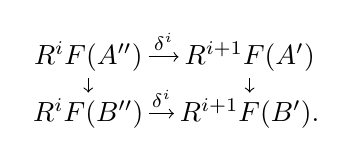
\begin{tikzpicture}[baseline=(current bounding box.center),inner sep=2pt]
  \node (a) at (0,.72) {$R^iF(A'')$};
  \node (b) at (2.05,.72) {$R^{i+1}F(A')$};
  \node (c) at (0,0) {$R^iF(B'')$};
  \node (d) at (2.05,0) {$R^{i+1}F(B')$.};
  \draw[->] (a) -- node[above] {$\scriptstyle\delta^i$} (b);
  \draw[->] (a) -- (c);
  \draw[->] (b) -- (d);
  \draw[->] (c) -- node[above] {$\scriptstyle\delta^i$} (d);
\end{tikzpicture}
\]
\item\hypertarget{result-III-1.1Ae}{} \emph{For each injective object $I$ of $\mathfrak A$, and for each $i>0$, we have $R^iF(I)=0$.}
\end{enumerate}

\par\smallskip\noindent\textbf{Definition.}\enspace With $F\colon\mathfrak A\to\mathfrak B$ as in the theorem, an object $J$ of $\mathfrak A$ is \emph{acyclic} for $F$ if $R^iF(J)=0$ for all $i>0$.

\AuditItem{result-III-1.2A}{Proposition 1.2A.} \emph{With $F\colon\mathfrak A\to\mathfrak B$ as in (\Goto{result-III-1.1A}{1.1A}), suppose there is an exact sequence}
\[
  0\to A\to J^0\to J^1\to\cdots
\]
\emph{where each $J^i$ is acyclic for $F$, $i\geqslant0$. (We say $J^\bullet$ is an $F$-}acyclic resolution \emph{of $A$.) Then for each $i\geqslant0$ there is a natural isomorphism $R^iF(A)\cong h^i(F(J^\bullet))$.}

\medskip
We leave to the reader the analogous definitions of projective objects, projective resolutions, an abelian category having enough projectives, and the left derived functors of a covariant right exact functor. Also, the right derived functors of a left exact contravariant functor (use projective resolutions) and the left derived functors of a right exact contravariant functor (use injective resolutions).

Next we will give a universal property of derived functors. For this purpose, we generalize slightly with the following definition.

\par\smallskip\noindent\textbf{Definition.}\enspace Let $\mathfrak A$ and $\mathfrak B$ be abelian categories. A (\emph{covariant}) \emph{$\delta$-functor} from $\mathfrak A$ to $\mathfrak B$ is a collection of functors $T=(T^i)_{i\geqslant0}$, together with a morphism $\delta^i\colon T^i(A'')\to T^{i+1}(A')$ for each short exact sequence $0\to A'\to A\to A''\to0$, and each $i\geqslant0$, such that:
\begin{enumerate}[label=(\arabic*),leftmargin=2.2em,itemsep=0pt,topsep=1pt,parsep=0pt]
\item For each short exact sequence as above, there is a long exact sequence
\[
\begin{gathered}
  0\to T^0(A')\to T^0(A)\to T^0(A'')
    \xrightarrow{\delta^0}T^1(A')\to\cdots\\
  \cdots\to T^i(A)\to T^i(A'')\xrightarrow{\delta^i}T^{i+1}(A')
    \to T^{i+1}(A)\to\cdots\ ; 
\end{gathered}
\]
\item for each morphism of one short exact sequence (as above) into another $0\to B'\to B\to B''\to0$, the $\delta$'s give a commutative diagram
\[
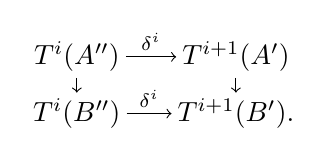
\begin{tikzpicture}[baseline=(current bounding box.center),inner sep=2pt]
  \node (a) at (0,.72) {$T^i(A'')$};
  \node (b) at (2.02,.72) {$T^{i+1}(A')$};
  \node (c) at (0,0) {$T^i(B'')$};
  \node (d) at (2.02,0) {$T^{i+1}(B')$.};
  \draw[->] (a) -- node[above] {$\scriptstyle\delta^i$} (b);
  \draw[->] (a) -- (c);
  \draw[->] (b) -- (d);
  \draw[->] (c) -- node[above] {$\scriptstyle\delta^i$} (d);
\end{tikzpicture}
\]
\end{enumerate}

\par\smallskip\noindent\textbf{Definition.}\enspace The $\delta$-functor $T=(T^i)\colon\mathfrak A\to\mathfrak B$ is said to be \emph{universal} if, given any other $\delta$-functor $T'=(T'^i)\colon\mathfrak A\to\mathfrak B$, and given any morphism of
}
% Contents from body/page-220.tex.
% Original printed page 206.
\BookMark{1}{3.2  Cohomology of Sheaves}{sec-III-2}
\ChapterSheet[11.35]{220}{206}{\Goto{p-215}{III\quad Cohomology}}{%
functors $f^0\colon T^0\to T'^0$, there exists a unique sequence of morphisms $f^i\colon T^i\to T'^i$ for each $i\geqslant0$, starting with the given $f^0$, which commute with the $\delta^i$ for each short exact sequence.

\AuditItem{result-III-1.2.1}{Remark 1.2.1.} If $F\colon\mathfrak A\to\mathfrak B$ is a covariant additive functor, then by definition there can exist at most one (up to unique isomorphism) universal $\delta$-functor $T$ with $T^0=F$. If $T$ exists, the $T^i$ are sometimes called the \emph{right satellite functors} of $F$.

\par\smallskip\noindent\textbf{Definition.}\enspace An additive functor $F\colon\mathfrak A\to\mathfrak B$ is \emph{effaceable} if for each object $A$ of $\mathfrak A$, there is a monomorphism $u\colon A\to M$, for some $M$, such that $F(u)=0$. It is \emph{coeffaceable} if for each $A$ there exists an epimorphism $u\colon P\to A$ such that $F(u)=0$.

\AuditItem{result-III-1.3A}{Theorem 1.3A.} \emph{Let $T=(T^i)_{i\geqslant0}$ be a covariant $\delta$-functor from $\mathfrak A$ to $\mathfrak B$. If $T^i$ is effaceable for each $i>0$, then $T$ is universal.}

\par\smallskip\noindent\textsc{Proof.}\enspace Grothendieck \Goto{bib-grothendieck-1}{[1, II, 2.2.1]}

\AuditItem{result-III-1.4}{Corollary 1.4.} \emph{Assume that $\mathfrak A$ has enough injectives. Then for any left exact functor $F\colon\mathfrak A\to\mathfrak B$, the derived functors $(R^iF)_{i\geqslant0}$ form a universal $\delta$-functor with $F\cong R^0F$. Conversely, if $T=(T^i)_{i\geqslant0}$ is any universal $\delta$-functor, then $T^0$ is left exact, and the $T^i$ are isomorphic to $R^iT^0$ for each $i\geqslant0$.}

\par\smallskip\noindent\textsc{Proof.}\enspace If $F$ is a left exact functor, then the $(R^iF)_{i\geqslant0}$ form a $\delta$-functor by (\Goto{result-III-1.1A}{1.1A}). Furthermore, for any object $A$, let $u\colon A\to I$ be a monomorphism of $A$ into an injective. Then $R^iF(I)=0$ for $i>0$ by (\Goto{result-III-1.1A}{1.1A}), so $R^iF(u)=0$. Thus $R^iF$ is effaceable for each $i>0$. It follows from the theorem that $(R^iF)$ is universal.

On the other hand, given a universal $\delta$-functor $T$, we have $T^0$ left exact by the definition of $\delta$-functor. Since $\mathfrak A$ has enough injectives, the derived functors $R^iT^0$ exist. We have just seen that $(R^iT^0)$ is another universal $\delta$-functor. Since $R^0T^0=T^0$, we find $R^iT^0\cong T^i$ for each $i$, by (\Goto{result-III-1.2.1}{1.2.1}).

\par\bigskip\noindent\hypertarget{sec-III-2}{}{\large\bfseries 2\enspace Cohomology of Sheaves}\par\medskip
\noindent In this section we define cohomology of sheaves by taking the derived functors of the global section functor. Then as an application of general techniques of cohomology we prove Grothendieck's theorem about the vanishing of cohomology on a noetherian topological space. To begin with, we must verify that the categories we use have enough injectives.

\AuditItem{result-III-2.1A}{Proposition 2.1A.} \emph{If $A$ is a ring, then every $A$-module is isomorphic to a submodule of an injective $A$-module.}

\par\smallskip\noindent\textsc{Proof.}\enspace Godement \Goto{bib-godement-1}{[1, I, 1.2.2]} or Hilton and Stammbach \Goto{bib-hilton-stammbach-1}{[1, I, 8.3]}.
}
% Contents from body/page-221.tex.
% Original printed page 207.
\ChapterSheet[11.35]{221}{207}{\Goto{sec-III-2}{2\quad Cohomology of Sheaves}}{%
\AuditItem{result-III-2.2}{Proposition 2.2.} \emph{Let $(X,\mathcal O_X)$ be a ringed space. Then the category $\mathfrak{Mod}(X)$ of sheaves of $\mathcal O_X$-modules has enough injectives.}

\par\smallskip\noindent\textsc{Proof.}\enspace Let $\mathcal F$ be a sheaf of $\mathcal O_X$-modules. For each point $x\in X$, the stalk $\mathcal F_x$ is an $\mathcal O_{X,x}$-module. Therefore there is an injection $\mathcal F_x\to I_x$, where $I_x$ is an injective $\mathcal O_{X,x}$-module (\Goto{result-III-2.1A}{2.1A}). For each point $x$, let $j$ denote the inclusion of the one-point space $\{x\}$ into $X$, and consider the sheaf $\mathcal I=\prod_{x\in X}j_*(I_x)$. Here we consider $I_x$ as a sheaf on the one-point space $\{x\}$, and $j_*$ is the direct image functor (II, \S\Goto{sec-II-1}{1}).

Now for any sheaf $\mathcal G$ of $\mathcal O_X$-modules, we have $\operatorname{Hom}_{\mathcal O_X}(\mathcal G,\mathcal I)=\prod\operatorname{Hom}_{\mathcal O_X}(\mathcal G,j_*(I_x))$ by definition of the direct product. On the other hand, for each point $x\in X$, we have $\operatorname{Hom}_{\mathcal O_X}(\mathcal G,j_*(I_x))\cong\operatorname{Hom}_{\mathcal O_{X,x}}(\mathcal G_x,I_x)$ as one sees easily. Thus we conclude first that there is a natural morphism of sheaves of $\mathcal O_X$-modules $\mathcal F\to\mathcal I$ obtained from the local maps $\mathcal F_x\to I_x$. It is clearly injective. Second, the functor $\operatorname{Hom}_{\mathcal O_X}(\cdot,\mathcal I)$ is the direct product over all $x\in X$ of the stalk functor $\mathcal G\mapsto\mathcal G_x$, which is exact, followed by $\operatorname{Hom}_{\mathcal O_{X,x}}(\cdot,I_x)$, which is exact, since $I_x$ is an injective $\mathcal O_{X,x}$-module. Hence $\operatorname{Hom}(\cdot,\mathcal I)$ is an exact functor, and therefore $\mathcal I$ is an injective $\mathcal O_X$-module.

\AuditItem{result-III-2.3}{Corollary 2.3.} \emph{If $X$ is any topological space, then the category $\mathfrak{Ab}(X)$ of sheaves of abelian groups on $X$ has enough injectives.}

\par\smallskip\noindent\textsc{Proof.}\enspace Indeed, if we let $\mathcal O_X$ be the constant sheaf of rings $\mathbf Z$, then $(X,\mathcal O_X)$ is a ringed space, and $\mathfrak{Mod}(X)=\mathfrak{Ab}(X)$.

\par\smallskip\noindent\textbf{Definition.}\enspace Let $X$ be a topological space. Let $\Gamma(X,\cdot)$ be the global section functor from $\mathfrak{Ab}(X)$ to $\mathfrak{Ab}$. We define the \emph{cohomology functors} $H^i(X,\cdot)$ to be the right derived functors of $\Gamma(X,\cdot)$. For any sheaf $\mathcal F$, the groups $H^i(X,\mathcal F)$ are the \emph{cohomology groups} of $\mathcal F$. Note that even if $X$ and $\mathcal F$ have some additional structure, e.g., $X$ a scheme and $\mathcal F$ a quasi-coherent sheaf, we always take cohomology in this sense, regarding $\mathcal F$ simply as a sheaf of abelian groups on the underlying topological space $X$.

We let the reader write out the long exact sequences which follow from the general properties of derived functors (\Goto{result-III-1.1A}{1.1A}).

\medskip
Recall (II, Ex.~\Goto{ex-II-1.16}{1.16}) that a sheaf $\mathcal F$ on a topological space $X$ is \emph{flasque} if for every inclusion of open sets $V\subseteq U$, the restriction map $\mathcal F(U)\to\mathcal F(V)$ is surjective.

\AuditItem{result-III-2.4}{Lemma 2.4.} \emph{If $(X,\mathcal O_X)$ is a ringed space, any injective $\mathcal O_X$-module is flasque.}

\par\smallskip\noindent\textsc{Proof.}\enspace For any open subset $U\subseteq X$, let $\mathcal O_U$ denote the sheaf $j_!(\mathcal O_X|_U)$, which is the restriction of $\mathcal O_X$ to $U$, extended by zero outside $U$ (II, Ex.~\Goto{ex-II-1.19}{1.19}). Now let $\mathcal I$ be an injective $\mathcal O_X$-module, and let $V\subseteq U$ be open sets. Then we have an inclusion $0\to\mathcal O_V\to\mathcal O_U$ of sheaves of $\mathcal O_X$-modules. Since $\mathcal I$ is injective, we get a surjection $\operatorname{Hom}(\mathcal O_U,\mathcal I)\to\operatorname{Hom}(\mathcal O_V,\mathcal I)\to0$. But $\operatorname{Hom}(\mathcal O_U,\mathcal I)=\mathcal I(U)$ and $\operatorname{Hom}(\mathcal O_V,\mathcal I)=\mathcal I(V)$, so $\mathcal I$ is flasque.
}
% Contents from body/page-222.tex.
% Original printed page 208.
\ChapterSheet[11.35]{222}{208}{\Goto{p-215}{III\quad Cohomology}}{%
\AuditItem{result-III-2.5}{Proposition 2.5.} \emph{If $\mathcal F$ is a flasque sheaf on a topological space $X$, then $H^i(X,\mathcal F)=0$ for all $i>0$.}

\par\smallskip\noindent\textsc{Proof.}\enspace Embed $\mathcal F$ in an injective object $\mathcal I$ of $\mathfrak{Ab}(X)$ and let $\mathcal G$ be the quotient:
\[
  0\to\mathcal F\to\mathcal I\to\mathcal G\to0.
\]
Then $\mathcal F$ is flasque by hypothesis, $\mathcal I$ is flasque by (\Goto{result-III-2.4}{2.4}), and so $\mathcal G$ is flasque by (II, Ex.~\Goto{ex-II-1.16c}{1.16c}). Now since $\mathcal F$ is flasque, we have an exact sequence (II, Ex.~\Goto{ex-II-1.16b}{1.16b})
\[
  0\to\Gamma(X,\mathcal F)\to\Gamma(X,\mathcal I)\to\Gamma(X,\mathcal G)\to0.
\]
On the other hand, since $\mathcal I$ is injective, we have $H^i(X,\mathcal I)=0$ for $i>0$ (\Goto{result-III-1.1Ae}{1.1Ae}). Thus from the long exact sequence of cohomology, we get $H^1(X,\mathcal F)=0$ and $H^i(X,\mathcal F)\cong H^{i-1}(X,\mathcal G)$ for each $i\geqslant2$. But $\mathcal G$ is also flasque, so by induction on $i$ we get the result.

\AuditItem{result-III-2.5.1}{Remark 2.5.1.} This result tells us that flasque sheaves are acyclic for the functor $\Gamma(X,\cdot)$. Hence we can calculate cohomology using flasque resolutions (\Goto{result-III-1.2A}{1.2A}). In particular, we have the following result.

\AuditItem{result-III-2.6}{Proposition 2.6.} \emph{Let $(X,\mathcal O_X)$ be a ringed space. Then the derived functors of the functor $\Gamma(X,\cdot)$ from $\mathfrak{Mod}(X)$ to $\mathfrak{Ab}$ coincide with the cohomology functors $H^i(X,\cdot)$.}

\par\smallskip\noindent\textsc{Proof.}\enspace Considering $\Gamma(X,\cdot)$ as a functor from $\mathfrak{Mod}(X)$ to $\mathfrak{Ab}$, we calculate its derived functors by taking injective resolutions in the category $\mathfrak{Mod}(X)$. But any injective is flasque (\Goto{result-III-2.4}{2.4}), and flasques are acyclic (\Goto{result-III-2.5}{2.5}) so this resolution gives the usual cohomology functors (\Goto{result-III-1.2A}{1.2A}).

\AuditItem{result-III-2.6.1}{Remark 2.6.1.} Let $(X,\mathcal O_X)$ be a ringed space, and let $A=\Gamma(X,\mathcal O_X)$. Then for any sheaf of $\mathcal O_X$-modules $\mathcal F$, $\Gamma(X,\mathcal F)$ has a natural structure of $A$-module. In particular, since we can calculate cohomology using resolutions in the category $\mathfrak{Mod}(X)$, all the cohomology groups of $\mathcal F$ have a natural structure of $A$-module; the associated exact sequences are sequences of $A$-modules, and so forth. Thus for example, if $X$ is a scheme over $\operatorname{Spec}B$ for some ring $B$, the cohomology groups of any $\mathcal O_X$-module $\mathcal F$ have a natural structure of $B$-module.

\medskip
\textit{A Vanishing Theorem of Grothendieck}

\par\noindent\hypertarget{result-III-2.7}{}\textbf{Theorem 2.7} (Grothendieck \Goto{bib-grothendieck-1}{[1]}). \emph{Let $X$ be a noetherian topological space of dimension $n$. Then for all $i>n$ and all sheaves of abelian groups $\mathcal F$ on $X$, we have $H^i(X,\mathcal F)=0$.}

\medskip
Before proving the theorem, we need some preliminary results, mainly concerning direct limits. If $(\mathcal F_\alpha)$ is a direct system of sheaves on $X$, indexed by a directed set $A$, then we have defined the direct limit $\varinjlim\mathcal F_\alpha$ (II, Ex.~\Goto{ex-II-1.10}{1.10}).
}
% Contents from body/page-223.tex.
% Original printed page 209.
\ChapterSheet[11.3]{223}{209}{\Goto{sec-III-2}{2\quad Cohomology of Sheaves}}{%
\AuditItem{result-III-2.8}{Lemma 2.8.} \emph{On a noetherian topological space, a direct limit of flasque sheaves is flasque.}

\par\smallskip\noindent\textsc{Proof.}\enspace Let $(\mathcal F_\alpha)$ be a directed system of flasque sheaves. Then for any inclusion of open sets $V\subseteq U$, and for each $\alpha$, we have $\mathcal F_\alpha(U)\to\mathcal F_\alpha(V)$ is surjective. Since $\varinjlim$ is an exact functor, we get
\[
  \varinjlim\mathcal F_\alpha(U)\to\varinjlim\mathcal F_\alpha(V)
\]
is also surjective. But on a noetherian topological space, $\varinjlim\mathcal F_\alpha(U)=(\varinjlim\mathcal F_\alpha)(U)$ for any open set (II, Ex.~\Goto{ex-II-1.11}{1.11}). So we have
\[
  (\varinjlim\mathcal F_\alpha)(U)\to(\varinjlim\mathcal F_\alpha)(V)
\]
is surjective, and so $\varinjlim\mathcal F_\alpha$ is flasque.

\AuditItem{result-III-2.9}{Proposition 2.9.} \emph{Let $X$ be a noetherian topological space, and let $(\mathcal F_\alpha)$ be a direct system of abelian sheaves. Then there are natural isomorphisms, for each $i\geqslant0$}
\[
  \varinjlim H^i(X,\mathcal F_\alpha)\to H^i(X,\varinjlim\mathcal F_\alpha).
\]

\noindent\textsc{Proof.}\enspace For each $\alpha$ we have a natural map $\mathcal F_\alpha\to\varinjlim\mathcal F_\alpha$. This induces a map on cohomology, and then we take the direct limit of these maps. For $i=0$, the result is already known (II, Ex.~\Goto{ex-II-1.11}{1.11}). For the general case, we consider the category $\mathfrak{ind}_A(\mathfrak{Ab}(X))$ consisting of all directed systems of objects of $\mathfrak{Ab}(X)$, indexed by $A$. This is an abelian category. Furthermore, since $\varinjlim$ is an exact functor, we have a natural transformation of $\delta$-functors
\[
  \varinjlim H^i(X,\cdot)\to H^i(X,\varinjlim\cdot)
\]
from $\mathfrak{ind}_A(\mathfrak{Ab}(X))$ to $\mathfrak{Ab}$. They agree for $i=0$, so to prove they are the same, it will be sufficient to show they are both effaceable for $i>0$. For in that case, they are both universal by (\Goto{result-III-1.3A}{1.3A}), and so must be isomorphic.

So let $(\mathcal F_\alpha)\in\mathfrak{ind}_A(\mathfrak{Ab}(X))$. For each $\alpha$, let $\mathcal G_\alpha$ be the sheaf of discontinuous sections of $\mathcal F_\alpha$ (II, Ex.~\Goto{ex-II-1.16e}{1.16e}). Then $\mathcal G_\alpha$ is flasque, and there is a natural inclusion $\mathcal F_\alpha\to\mathcal G_\alpha$. Furthermore, the construction of $\mathcal G_\alpha$ is functorial, so the $\mathcal G_\alpha$ also form a direct system, and we obtain a monomorphism $u\colon(\mathcal F_\alpha)\to(\mathcal G_\alpha)$ in the category $\mathfrak{ind}_A(\mathfrak{Ab}(X))$. Now the $\mathcal G_\alpha$ are all flasque, so $H^i(X,\mathcal G_\alpha)=0$ for $i>0$ (\Goto{result-III-2.5}{2.5}). Thus $\varinjlim H^i(X,\mathcal G_\alpha)=0$, and the functor on the left-hand side is effaceable for $i>0$. On the other hand, $\varinjlim\mathcal G_\alpha$ is also flasque by (\Goto{result-III-2.8}{2.8}). So $H^i(X,\varinjlim\mathcal G_\alpha)=0$ for $i>0$, and we see that the functor on the right-hand side is also effaceable. This completes the proof.

\AuditItem{result-III-2.9.1}{Remark 2.9.1.} As a special case we see that cohomology commutes with infinite direct sums.

\AuditItem{result-III-2.10}{Lemma 2.10.} \emph{Let $Y$ be a closed subset of $X$, let $\mathcal F$ be a sheaf of abelian groups on $Y$, and let $j\colon Y\to X$ be the inclusion. Then $H^i(Y,\mathcal F)=H^i(X,j_*\mathcal F)$, where $j_*\mathcal F$ is the extension of $\mathcal F$ by zero outside $Y$} (II, Ex.~\Goto{ex-II-1.19}{1.19}).
}
% Contents from body/page-224.tex.
% Original printed page 210.
\ChapterSheet[11.35]{224}{210}{\Goto{p-215}{III\quad Cohomology}}{%
\textsc{Proof.}\enspace If $\mathcal I^\bullet$ is a flasque resolution of $\mathcal F$ on $Y$, then $j_*\mathcal I^\bullet$ is a flasque resolution of $j_*\mathcal F$ on $X$, and for each $i$, $\Gamma(Y,\mathcal I^i)=\Gamma(X,j_*\mathcal I^i)$. So we get the same cohomology groups.

\AuditItem{result-III-2.10.1}{Remark 2.10.1.} Continuing our earlier abuse of notation (II, Ex.~\Goto{ex-II-1.19}{1.19}), we often write $\mathcal F$ instead of $j_*\mathcal F$. This lemma shows there will be no ambiguity about the cohomology groups.

\par\smallskip\noindent\textsc{Proof of} (\Goto{result-III-2.7}{2.7}). First we fix some notation. If $Y$ is a closed subset of $X$, then for any sheaf $\mathcal F$ on $X$ we let $\mathcal F_Y=j_*(\mathcal F|_Y)$, where $j\colon Y\to X$ is the inclusion. If $U$ is an open subset of $X$, we let $\mathcal F_U=i_!(\mathcal F|_U)$, where $i\colon U\to X$ is the inclusion. In particular, if $U=X-Y$, we have an exact sequence (II, Ex.~\Goto{ex-II-1.19}{1.19})
\[
  0\to\mathcal F_U\to\mathcal F\to\mathcal F_Y\to0.
\]

We will prove the theorem by induction on $n=\dim X$, in several steps.

\emph{Step 1.} Reduction to the case $X$ irreducible. If $X$ is reducible, let $Y$ be one of its irreducible components, and let $U=X-Y$. Then for any $\mathcal F$ we have an exact sequence
\[
  0\to\mathcal F_U\to\mathcal F\to\mathcal F_Y\to0.
\]
From the long exact sequence of cohomology, it will be sufficient to prove that $H^i(X,\mathcal F_Y)=0$ and $H^i(X,\mathcal F_U)=0$ for $i>n$. But $Y$ is closed and irreducible, and $\mathcal F_U$ can be regarded as a sheaf on the closed subset $\bar U$, which has one fewer irreducible components than $X$. Thus using (\Goto{result-III-2.10}{2.10}) and induction on the number of irreducible components, we reduce to the case $X$ irreducible.

\emph{\EditionText{Step 2.}} Suppose $X$ is irreducible of dimension $0$. Then the only open subsets of $X$ are $X$ and the empty set. For otherwise, $X$ would have a proper irreducible closed subset, and $\dim X$ would be $\geqslant1$. Thus $\Gamma(X,\cdot)$ induces an equivalence of categories $\mathfrak{Ab}(X)\to\mathfrak{Ab}$. In particular, $\Gamma(X,\cdot)$ is an exact functor, so $H^i(X,\mathcal F)=0$ for $i>0$, and for all $\mathcal F$.

\emph{Step 3.} Now let $X$ be irreducible of dimension $n$, and let $\mathcal F\in\mathfrak{Ab}(X)$. Let \EditionText{$B=\coprod_{U\subseteq X\text{ open}}\mathcal F(U)$}, and let $A$ be the set of all finite subsets of $B$. For each $\alpha\in A$, let $\mathcal F_\alpha$ be the subsheaf of $\mathcal F$ generated by the sections in $\alpha$ (over various open sets). Then $A$ is a directed set, and $\mathcal F=\varinjlim\mathcal F_\alpha$. So by (\Goto{result-III-2.9}{2.9}), it will be sufficient to prove vanishing of cohomology for each $\mathcal F_\alpha$. If $\alpha'$ is a subset of $\alpha$, then we have an exact sequence
\[
  0\to\mathcal F_{\alpha'}\to\mathcal F_\alpha\to\mathcal G\to0,
\]
where $\mathcal G$ is a sheaf generated by $\#(\alpha-\alpha')$ sections over suitable open sets. Thus, using the long exact sequence of cohomology, and induction on $\#(\alpha)$, we reduce to the case that $\mathcal F$ is generated by a single section over some open set $U$. In that case $\mathcal F$ is a quotient of the sheaf $\mathbf Z_U$ (where $\mathbf Z$ denotes the constant sheaf $\mathbf Z$ on $X$). Letting $\mathcal R$ be the kernel, we have an exact sequence
\[
  0\to\mathcal R\to\mathbf Z_U\to\mathcal F\to0.
\]
}
% Contents from body/page-225.tex.
% Original printed page 211.
\ChapterSheet[11.35]{225}{211}{\Goto{sec-III-2}{2\quad Cohomology of Sheaves}}{%
Again using the long exact sequence of cohomology, it will be sufficient to prove vanishing for $\mathcal R$ and for $\mathbf Z_U$.

\emph{Step 4.} Let $U$ be an open subset of $X$ and let $\mathcal R$ be a subsheaf of $\mathbf Z_U$. For each $x\in U$, the stalk $\mathcal R_x$ is a subgroup of $\mathbf Z$. If $\mathcal R=0$, skip to Step \Goto{proof-III-2.7-step-5}{5}. If not, let $d$ be the least positive integer which occurs in any of the groups $\mathcal R_x$. Then there is a nonempty open subset $V\subseteq U$ such that $\mathcal R|_V\cong d\cdot\mathbf Z|_V$ as a subsheaf of $\mathbf Z|_V$. Thus $\mathcal R_V\cong\mathbf Z_V$ and we have an exact sequence
\[
  0\to\mathbf Z_V\to\mathcal R\to\mathcal R/\mathbf Z_V\to0.
\]
Now the sheaf $\mathcal R/\mathbf Z_V$ is supported on the closed subset $\overline{(U-V)}$ of $X$, which has dimension $<n$, since $X$ is irreducible. So using (\Goto{result-III-2.10}{2.10}) and the induction hypothesis, we know $H^i(X,\mathcal R/\mathbf Z_V)=0$ for $i\geqslant n$. So by the long exact sequence of cohomology, we need only show vanishing for $\mathbf Z_V$.

\hypertarget{proof-III-2.7-step-5}{}\emph{Step 5.} To complete the proof, we need only show that for any open subset $U\subseteq X$, we have $H^i(X,\mathbf Z_U)=0$ for $i>n$. Let $Y=X-U$. Then we have an exact sequence
\[
  0\to\mathbf Z_U\to\mathbf Z\to\mathbf Z_Y\to0.
\]
Now $\dim Y<\dim X$ since $X$ is irreducible, so using (\Goto{result-III-2.10}{2.10}) and the induction hypothesis, we have $H^i(X,\mathbf Z_Y)=0$ for $i\geqslant n$. On the other hand, $\mathbf Z$ is flasque, since it is a constant sheaf on an irreducible space (II, Ex.~\Goto{ex-II-1.16a}{1.16a}). Hence $H^i(X,\mathbf Z)=0$ for $i>0$ by (\Goto{result-III-2.5}{2.5}). So from the long exact sequence of cohomology we have $H^i(X,\mathbf Z_U)=0$ for $i>n$.\nobreak\hfill q.e.d.

\medskip
\emph{Historical Note:} The derived functor cohomology which we defined in this section was introduced by Grothendieck \Goto{bib-grothendieck-1}{[1]}. It is the theory which is used in \Goto{bib-EGA}{[EGA]}. The use of sheaf cohomology in algebraic geometry started with Serre \Goto{bib-serre-3}{[3]}. In that paper, and in the later paper \Goto{bib-serre-4}{[4]}, Serre used \v{C}ech cohomology for coherent sheaves on an algebraic variety with its Zariski topology. The equivalence of this theory with the derived functor theory follows from the \textquotedblleft theorem of Leray\textquotedblright\ (Ex.~\Goto{ex-III-4.11}{4.11}). The same argument, using Cartan's \textquotedblleft Theorem B\textquotedblright\ shows that the \v{C}ech cohomology of a coherent analytic sheaf on a complex analytic space is equal to the derived functor cohomology. Gunning and Rossi \Goto{bib-gunning-rossi-1}{[1]} use a cohomology theory computed by fine resolutions of a sheaf on a paracompact Hausdorff space. The equivalence of this theory with ours is shown by Godement \Goto{bib-godement-1}{[1, Thm.~4.7.1, p.~181 and Ex.~7.2.1, p.~263]}, who shows at the same time that both theories coincide with his theory which is defined by a canonical flasque resolution. Godement also shows \Goto{bib-godement-1}{[1, Thm.~5.10.1, p.~228]} that on a paracompact Hausdorff space, his theory coincides with \v{C}ech cohomology. This provides a bridge to the standard topological theories with constant coefficients, as developed in the book of Spanier \Goto{bib-spanier-1}{[1]}. \EditionText{On a paracompact Hausdorff space, \v{C}ech and Alexander--Spanier cohomology with constant coefficients agree. They also agree with singular cohomology if the space is homologically locally connected, in particular if it is locally contractible (see Spanier \Goto{bib-spanier-1}{[1, \S6.8 and Corollary~6.9.5]}).}
}
% Contents from body/page-226.tex.
% Original printed page 212.
\ChapterSheet[10.95]{226}{212}{\Goto{p-215}{III\quad Cohomology}}{%
\indent The vanishing theorem (\Goto{result-III-2.7}{2.7}) was proved by Serre \Goto{bib-serre-3}{[3]} for coherent sheaves on algebraic curves and projective algebraic varieties, and later \Goto{bib-serre-5}{[5]} for abstract algebraic varieties. It is analogous to the theorem that singular cohomology on a (real) manifold of dimension $n$ vanishes in degrees $i>n$.

\par\medskip\noindent\textsc{Exercises}\par

\AuditItem{ex-III-2.1}{2.1.} (a) Let $X=\mathbf A^1_k$ be the affine line over an infinite field $k$. Let $P,Q$ be distinct closed points of $X$, and let $U=X-\{P,Q\}$. Show that $H^1(X,\mathbf Z_U)\ne0$.

\noindent\hangindent=3em\hspace*{1.35em}*(b) More generally, let $Y\subseteq X=\mathbf A_k^n$ be the union of $n+1$ hyperplanes in suitably general position, and let $U=X-Y$. Show that $H^n(X,\mathbf Z_U)\ne0$. Thus the result of (\Goto{result-III-2.7}{2.7}) is the best possible.

\AuditItem{ex-III-2.2}{2.2.} Let $X=\mathbf P_k^1$ be the projective line over an algebraically closed field $k$. Show that the exact sequence $0\to\mathcal O\to\mathcal K\to\mathcal K/\mathcal O\to0$ of (II, Ex.~\Goto{ex-II-1.21d}{1.21d}) is a flasque resolution of $\mathcal O$. Conclude from (II, Ex.~\Goto{ex-II-1.21e}{1.21e}) that $H^i(X,\mathcal O)=0$ for all $i>0$.

\AuditItem{ex-III-2.3}{2.3.} \emph{Cohomology with Supports} (Grothendieck \Goto{bib-grothendieck-7}{[7]}). Let $X$ be a topological space, let $Y$ be a closed subset, and let $\mathcal F$ be a sheaf of abelian groups. Let $\Gamma_Y(X,\mathcal F)$ denote the group of sections of $\mathcal F$ with support in $Y$ (II, Ex.~\Goto{ex-II-1.20}{1.20}).
\begin{enumerate}[label=(\alph*),leftmargin=2.5em,itemsep=0pt,topsep=1pt,parsep=0pt]
\item Show that $\Gamma_Y(X,\cdot)$ is a left exact functor from $\mathfrak{Ab}(X)$ to $\mathfrak{Ab}$.

We denote the right derived functors of $\Gamma_Y(X,\cdot)$ by $H_Y^i(X,\cdot)$. They are the \emph{cohomology groups of $X$ with supports in $Y$}, and coefficients in a given sheaf.
\item If $0\to\mathcal F'\to\mathcal F\to\mathcal F''\to0$ is an exact sequence of sheaves, with $\mathcal F'$ flasque, show that
\[
  0\to\Gamma_Y(X,\mathcal F')\to\Gamma_Y(X,\mathcal F)\to\Gamma_Y(X,\mathcal F'')\to0
\]
is exact.
\item Show that if $\mathcal F$ is flasque, then $H_Y^i(X,\mathcal F)=0$ for all $i>0$.
\item If $\mathcal F$ is flasque, show that the sequence
\[
  0\to\Gamma_Y(X,\mathcal F)\to\Gamma(X,\mathcal F)\to\Gamma(X-Y,\mathcal F)\to0
\]
is exact.
\item Let $U=X-Y$. Show that for any $\mathcal F$, there is a long exact sequence of cohomology groups
\[
\begin{aligned}
  0&\to H_Y^0(X,\mathcal F)\to H^0(X,\mathcal F)\to H^0(U,\mathcal F|_U)\to\\
   &\to H_Y^1(X,\mathcal F)\to H^1(X,\mathcal F)\to H^1(U,\mathcal F|_U)\to\\
   &\to H_Y^2(X,\mathcal F)\to\cdots.
\end{aligned}
\]
\item \emph{Excision.} Let $V$ be an open subset of $X$ containing $Y$. Then there are natural functorial isomorphisms, for all $i$ and $\mathcal F$,
\[
  H_Y^i(X,\mathcal F)\cong H_Y^i(V,\mathcal F|_V).
\]
\end{enumerate}

\AuditItem{ex-III-2.4}{2.4.} \emph{Mayer--Vietoris Sequence.} Let $Y_1,Y_2$ be two closed subsets of $X$. Then there is a long exact sequence of cohomology with supports
\[
\begin{aligned}
  \cdots\to &H^i_{Y_1\cap Y_2}(X,\mathcal F)
  \to H^i_{Y_1}(X,\mathcal F)\oplus H^i_{Y_2}(X,\mathcal F)
  \to H^i_{Y_1\cup Y_2}(X,\mathcal F)\to\\
  \to &H^{i+1}_{Y_1\cap Y_2}(X,\mathcal F)\to\cdots.
\end{aligned}
\]
}
% Contents from body/page-227.tex.
% Original printed page 213.
\BookMark{1}{3.3  Cohomology of a Noetherian Affine Scheme}{sec-III-3}
\ChapterSheet[10.95]{227}{213}{\Goto{sec-III-3}{3\quad Cohomology of a Noetherian Affine Scheme}}{%
\AuditItem{ex-III-2.5}{2.5.} Let $X$ be a Zariski space (II, Ex.~\Goto{ex-II-3.17}{3.17}). Let $P\in X$ be a closed point, and let $X_P$ be the subset of $X$ consisting of all points $Q\in X$ such that $P\in\overline{\{Q\}}$. We call $X_P$ the \emph{local space of $X$ at $P$}, and give it the induced topology. Let $j\colon X_P\to X$ be the inclusion, and for any sheaf $\mathcal F$ on $X$, let $\mathcal F_P=j^*\mathcal F$. Show that for all $i$, $\mathcal F$, we have
\[
  H_P^i(X,\mathcal F)=H_P^i(X_P,\mathcal F_P).
\]

\AuditItem{ex-III-2.6}{2.6.} Let $X$ be a noetherian topological space, and let $\{\mathcal I_\alpha\}_{\alpha\in A}$ be a direct system of injective sheaves of abelian groups on $X$. Then $\varinjlim\mathcal I_\alpha$ is also injective. [\emph{Hints:} First show that a sheaf $\mathcal I$ is injective if and only if for every open set $U\subseteq X$, and for every subsheaf $\mathcal R\subseteq\mathbf Z_U$, and for every map $f\colon\mathcal R\to\mathcal I$, there exists an extension of $f$ to a map $\mathbf Z_U\to\mathcal I$. Secondly, \EditionText{show that $\mathbf Z_U$ is noetherian. Present $\mathcal R$ using finitely many generators and relations from finite direct sums of sheaves $\mathbf Z_V$ with $V$ open in $X$. Then any map $\mathcal R\to\varinjlim\mathcal I_\alpha$ factors through one of the $\mathcal I_\alpha$.}]

\AuditItem{ex-III-2.7}{2.7.} Let $S^1$ be the circle (with its usual topology), and let $\mathbf Z$ be the constant sheaf $\mathbf Z$.
\begin{enumerate}[label=(\alph*),leftmargin=2.5em,itemsep=0pt,topsep=1pt,parsep=0pt]
\item Show that $H^1(S^1,\mathbf Z)\cong\mathbf Z$, using our definition of cohomology.
\item Now let $\mathcal R$ be the sheaf of germs of continuous real-valued functions on $S^1$. Show that $H^1(S^1,\mathcal R)=0$.
\end{enumerate}

\par\bigskip\noindent\hypertarget{sec-III-3}{}{\large\bfseries 3\enspace Cohomology of a Noetherian Affine Scheme}\par\medskip
\noindent In this section we will prove that if $X=\operatorname{Spec}A$ is a noetherian affine scheme, then $H^i(X,\mathcal F)=0$ for all $i>0$ and all quasi-coherent sheaves $\mathcal F$ of $\mathcal O_X$-modules. The key point is to show that if $I$ is an injective $A$-module, then the sheaf $\widetilde I$ on $\operatorname{Spec}A$ is flasque. We begin with some algebraic preliminaries.

\par\smallskip\noindent\hypertarget{result-III-3.1A}{}\textbf{Proposition 3.1A} (Krull's Theorem). \emph{Let $A$ be a noetherian ring, let $M\subseteq N$ be finitely generated $A$-modules, and let $\mathfrak a$ be an ideal of $A$. Then the $\mathfrak a$-adic topology on $M$ is induced by the $\mathfrak a$-adic topology on $N$. In particular, for any $n>0$, there exists an $n'\geqslant n$ such that $\mathfrak a^nM\supseteq M\cap\mathfrak a^{n'}N$.}

\par\noindent\textsc{Proof.}\enspace Atiyah--Macdonald \Goto{bib-atiyah-macdonald-1}{[1, 10.11]} or Zariski--Samuel \Goto{bib-zariski-samuel-1}{[1, vol.~II, Ch.~VIII, Th.~4]}.

\medskip
Recall (II, Ex.~\Goto{ex-II-5.6}{5.6}) that for any ring $A$, and any ideal $\mathfrak a\subseteq A$, and any $A$-module $M$, we have defined the submodule $\Gamma_{\mathfrak a}(M)$ to be $\{m\in M\mid\mathfrak a^nm=0\text{ for some }n>0\}$.

\AuditItem{result-III-3.2}{Lemma 3.2.} \emph{Let $A$ be a noetherian ring, let $\mathfrak a$ be an ideal of $A$, and let $I$ be an injective $A$-module. Then the submodule $J=\Gamma_{\mathfrak a}(I)$ is also an injective $A$-module.}

\par\smallskip\noindent\textsc{Proof.}\enspace To show that $J$ is injective, it will be sufficient to show that for any ideal $\mathfrak b\subseteq A$, and for any homomorphism $\varphi\colon\mathfrak b\to J$, there exists a homomorphism $\psi\colon A\to J$ extending $\varphi$. (This is a well-known criterion for an injective module---Godement \Goto{bib-godement-1}{[1, I, 1.4.1]}). Since $A$ is noetherian, $\mathfrak b$ is finitely generated. On the other hand, every element of $J$ is annihilated by some
}
% Contents from body/page-228.tex.
\usetikzlibrary{arrows}
\ChapterSheet{228}{214}{\Goto{p-215}{III\quad Cohomology}}{%
power of $\mathfrak a$, so there exists an $n>0$ such that $\mathfrak a^n\varphi(\mathfrak b)=0$, or equivalently, $\varphi(\mathfrak a^n\mathfrak b)=0$. Now applying \Goto{result-III-3.1A}{(3.1A)} to the inclusion $\mathfrak b\subseteq A$, we find that there is an $n'\geq n$ such that $\mathfrak a^n\mathfrak b\supseteq\mathfrak b\cap\mathfrak a^{n'}$. Hence $\varphi(\mathfrak b\cap\mathfrak a^{n'})=0$, and so the map $\varphi\colon\mathfrak b\to J$ factors through $\mathfrak b/(\mathfrak b\cap\mathfrak a^{n'})$. Now we consider the following diagram:
\[
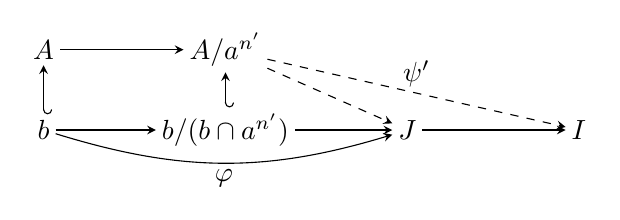
\begin{tikzpicture}[x=1.65cm,y=1.02cm,every node/.style={inner sep=2pt},>=stealth]
\node (a) at (0,0) {$A$};
\node (aq) at (1.4,0) {$A/\mathfrak a^{n'}$};
\node (b) at (0,-1) {$\mathfrak b$};
\node (bq) at (1.4,-1) {$\mathfrak b/(\mathfrak b\cap\mathfrak a^{n'})$};
\node (j) at (2.8,-1) {$J$};
\node (i) at (4.12,-1) {$I$};
\draw[->] (a) -- (aq);
\draw[left hook-stealth] (b) -- (a);
\draw[left hook-stealth] (bq) -- (aq);
\draw[->] (b) -- (bq);
\draw[->] (bq) -- (j);
\draw[->] (j) -- (i);
\draw[dashed,->] (aq) -- (j);
\draw[dashed,->] (aq) -- node[above] {$\psi'$} (i);
\draw[->] (b) to[bend right=17] node[below] {$\varphi$} (j);
\end{tikzpicture}
\]
Since $I$ is injective, the composed map of $\mathfrak b/(\mathfrak b\cap\mathfrak a^{n'})$ to $I$ extends to a map $\psi'\colon A/\mathfrak a^{n'}\to I$. But the image of $\psi'$ is annihilated by $\mathfrak a^{n'}$, so it is contained in $J$. Composing with the natural map $A\to A/\mathfrak a^{n'}$, we obtain the required map $\psi\colon A\to J$ extending $\varphi$.

\medskip
\noindent\hypertarget{result-III-3.3}{}\textbf{Lemma 3.3.} \emph{Let $I$ be an injective module over a noetherian ring $A$. Then for any $f\in A$, the natural map of $I$ to its localization $I_f$ is surjective.}

\smallskip
\noindent\textsc{Proof.} For each $i>0$, let $\mathfrak b_i$ be the annihilator of $f^i$ in $A$. Then $\mathfrak b_1\subseteq\mathfrak b_2\subseteq\cdots$, and since $A$ is noetherian, there is an $r$ such that $\mathfrak b_r=\mathfrak b_{r+1}=\cdots$. Now let $\theta\colon I\to I_f$ be the natural map, and let $x\in I_f$ be any element. Then by definition of localization, there is a $y\in I$ and an $n\geq0$ such that $x=\theta(y)/f^n$. We define a map $\varphi$ from the ideal $(f^{n+r})$ of $A$ to $I$ by sending $f^{n+r}$ to $f^ry$. This is possible, because the annihilator of $f^{n+r}$ is $\mathfrak b_{n+r}=\mathfrak b_r$, and $\mathfrak b_r$ annihilates $f^ry$. Since $I$ is injective, $\varphi$ extends to a map $\psi\colon A\to I$. Let $\psi(1)=z$. Then $f^{n+r}z=f^ry$. But this implies that $\theta(z)=\theta(y)/f^n=x$. Hence $\theta$ is surjective.

\medskip
\noindent\hypertarget{result-III-3.4}{}\textbf{Proposition 3.4.} \emph{Let $I$ be an injective module over a noetherian ring $A$. Then the sheaf $\widetilde I$ on $X=\operatorname{Spec}A$ is flasque.}

\smallskip
\noindent\textsc{Proof.} We will use noetherian induction on $Y=(\operatorname{Supp}\widetilde I)^{-}$. See (II, Ex.~\Goto{ex-II-1.14}{1.14}) for the notion of support. If $Y$ consists of a single closed point of $X$, then $\widetilde I$ is a skyscraper sheaf (II, Ex.~\Goto{ex-II-1.17}{1.17}) which is obviously flasque.

In the general case, to show that $\widetilde I$ is flasque, it will be sufficient to show, for any open set $U\subseteq X$, that $\Gamma(X,\widetilde I)\to\Gamma(U,\widetilde I)$ is surjective. If $Y\cap U=\varnothing$, there is nothing to prove. If $Y\cap U\ne\varnothing$, we can find an $f\in A$ such that the open set $X_f=D(f)$ (II, \Goto{sec-II-2}{\S2}) is contained in $U$ and $X_f\cap Y\ne\varnothing$. Let $Z=X-X_f$, and consider the following diagram:
\[
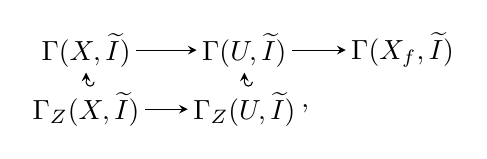
\begin{tikzpicture}[x=2.01cm,y=.75cm,every node/.style={inner sep=1.8pt},>=stealth]
\node (x) at (0,0) {$\Gamma(X,\widetilde I)$};
\node (u) at (1,0) {$\Gamma(U,\widetilde I)$};
\node (f) at (2,0) {$\Gamma(X_f,\widetilde I)$};
\node (xz) at (0,-1) {$\Gamma_Z(X,\widetilde I)$};
\node (uz) at (1,-1) {$\Gamma_Z(U,\widetilde I)$};
\draw[->] (x) -- (u);
\draw[->] (u) -- (f);
\draw[->] (xz) -- (uz);
\draw[left hook-stealth] (xz) -- (x);
\draw[left hook-stealth] (uz) -- (u);
\node[anchor=west,inner sep=0pt] at (uz.east) {$,$};
\end{tikzpicture}
\]
}
% Contents from body/page-229.tex.
\ChapterSheet{229}{215}{\Goto{sec-III-3}{3\quad Cohomology of a Noetherian Affine Scheme}}{%
where $\Gamma_Z$ denotes sections with support in $Z$ (II, Ex.~\Goto{ex-II-1.20}{1.20}). Now given a section $s\in\Gamma(U,\widetilde I)$, we consider its image $s'$ in $\Gamma(X_f,\widetilde I)$. But $\Gamma(X_f,\widetilde I)=I_f$ (II, \Goto{result-II-5.1}{5.1}), so by \Goto{result-III-3.3}{(3.3)}, there is a $t\in I=\Gamma(X,\widetilde I)$ restricting to $s'$. Let $t'$ be the restriction of $t$ to $\Gamma(U,\widetilde I)$. Then $s-t'$ goes to $0$ in $\Gamma(X_f,\widetilde I)$, so it has support in $Z$. Thus to complete the proof, it will be sufficient to show that $\Gamma_Z(X,\widetilde I)\to\Gamma_Z(U,\widetilde I)$ is surjective.

Let $J=\Gamma_Z(X,\widetilde I)$. If $\mathfrak a$ is the ideal generated by $f$, then $J=\Gamma_{\mathfrak a}(I)$ (II, Ex.~\Goto{ex-II-5.6}{5.6}), so by \Goto{result-III-3.2}{(3.2)}, $J$ is also an injective $A$-module. Furthermore, the support of $\widetilde J$ is contained in $Y\cap Z$, which is strictly smaller than $Y$. Hence by our induction hypothesis, $\widetilde J$ is flasque. Since $\Gamma(U,\widetilde J)=\Gamma_Z(U,\widetilde I)$ (II, Ex.~\Goto{ex-II-5.6}{5.6}), we conclude that $\Gamma_Z(X,\widetilde I)\to\Gamma_Z(U,\widetilde I)$ is surjective, as required.

\medskip
\noindent\hypertarget{result-III-3.5}{}\textbf{Theorem 3.5.} \emph{Let $X=\operatorname{Spec}A$ be the spectrum of a noetherian ring $A$. Then for all quasi-coherent sheaves $\mathcal F$ on $X$, and for all $i>0$, we have $H^i(X,\mathcal F)=0$.}

\smallskip
\noindent\textsc{Proof.} Given $\mathcal F$, let $M=\Gamma(X,\mathcal F)$, and take an injective resolution $0\to M\to I^\bullet$ of $M$ in the category of $A$-modules. Then we obtain an exact sequence of sheaves $0\to\widetilde M\to\widetilde I^\bullet$ on $X$. Now $\mathcal F=\widetilde M$ (II, \Goto{result-II-5.5}{5.5}) and each $\widetilde I^i$ is flasque by \Goto{result-III-3.4}{(3.4)}, so we can use this resolution of $\mathcal F$ to calculate cohomology \Goto{result-III-2.5.1}{(2.5.1)}. Applying the functor $\Gamma$, we recover the exact sequence of $A$-modules $0\to M\to I^\bullet$. Hence $H^0(X,\mathcal F)=M$, and $H^i(X,\mathcal F)=0$ for $i>0$.

\medskip
\noindent\hypertarget{result-III-3.5.1}{}\textbf{Remark 3.5.1.} This result is also true without the noetherian hypothesis, but the proof is more difficult \Goto{bib-ega-iii}{[EGA III, 1.3.1]}.

\medskip
\noindent\hypertarget{result-III-3.6}{}\textbf{Corollary 3.6.} \emph{Let $X$ be a noetherian scheme, and let $\mathcal F$ be a quasi-coherent sheaf on $X$. Then $\mathcal F$ can be embedded in a flasque, quasi-coherent sheaf $\mathcal G$.}

\smallskip
\noindent\textsc{Proof.} Cover $X$ with a finite number of open affines $U_i=\operatorname{Spec}A_i$, and let $\mathcal F|_{U_i}=\widetilde M_i$ for each $i$. Embed $M_i$ in an injective module $I_i$. For each $i$, let $f\colon U_i\to X$ be the inclusion, and let $\mathcal G=\bigoplus f_*(\widetilde I_i)$. For each $i$ we have an injective map of sheaves $\mathcal F|_{U_i}\to\widetilde I_i$. Hence we obtain a map $\mathcal F\to f_*(\widetilde I_i)$. Taking the direct sum over $i$ gives a map $\mathcal F\to\mathcal G$ which is clearly injective. On the other hand, for each $i$, $\widetilde I_i$ is flasque \Goto{result-III-3.4}{(3.4)} and quasi-coherent on $U_i$. Hence $f_*(\widetilde I_i)$ is also flasque (II, Ex.~\Goto{ex-II-1.16}{1.16d}) and quasi-coherent (II, \Goto{result-II-5.8}{5.8}). Taking the direct sum of these, we see that $\mathcal G$ is flasque and quasi-coherent.

\medskip
\noindent\hypertarget{result-III-3.7}{}\textbf{Theorem 3.7} (Serre \Goto{bib-serre-5}{[5]}). \emph{Let $X$ be a noetherian scheme. Then the following conditions are equivalent:}
\par{\itshape\leftskip=12pt
\hypertarget{result-III-3.7-i}{}(i) $X$ is affine;

\hypertarget{result-III-3.7-ii}{}(ii) $H^i(X,\mathcal F)=0$ for all $\mathcal F$ quasi-coherent and all $i>0$;

\hypertarget{result-III-3.7-iii}{}(iii) $H^1(X,\mathcal I)=0$ for all coherent sheaves of ideals $\mathcal I$.\par}

\smallskip
\noindent\textsc{Proof.} \Goto{result-III-3.7-i}{(i)} $\Rightarrow$ \Goto{result-III-3.7-ii}{(ii)} is \Goto{result-III-3.5}{(3.5)}. \Goto{result-III-3.7-ii}{(ii)} $\Rightarrow$ \Goto{result-III-3.7-iii}{(iii)} is trivial, so we have only to prove \Goto{result-III-3.7-iii}{(iii)} $\Rightarrow$ \Goto{result-III-3.7-i}{(i)}. We use the criterion of (II, Ex.~\Goto{ex-II-2.17}{2.17}). First we show that $X$ can
}
% Contents from body/page-230.tex.
\ChapterSheet{230}{216}{\Goto{p-215}{III\quad Cohomology}}{%
be covered by open affine subsets of the form $X_f$, with $f\in A=\Gamma(X,\mathcal O_X)$. Let $P$ be a closed point of $X$, let $U$ be an open affine neighborhood of $P$, and let $Y=X-U$. Then we have an exact sequence
\[
0\to\mathcal I_{Y\cup\{P\}}\to\mathcal I_Y\to k(P)\to0,
\]
where $\mathcal I_Y$ and $\mathcal I_{Y\cup\{P\}}$ are the ideal sheaves of the closed sets $Y$ and $Y\cup\{P\}$, respectively. The quotient is the skyscraper sheaf $k(P)=\mathcal O_P/\mathfrak m_P$ at $P$. Now from the exact sequence of cohomology, and hypothesis \Goto{result-III-3.7-iii}{(iii)}, we get an exact sequence
\[
\Gamma(X,\mathcal I_Y)\to\Gamma(X,k(P))\to H^1(X,\mathcal I_{Y\cup\{P\}})=0.
\]
So there is an element $f\in\Gamma(X,\mathcal I_Y)$ which goes to $1$ in $k(P)$, i.e., $f_P\equiv1$ (mod $\mathfrak m_P$). Since $\mathcal I_Y\subseteq\mathcal O_X$, we can consider $f$ as an element of $A$. Then by construction, we have $P\in X_f\subseteq U$. Furthermore, $X_f=U_{\bar f}$, where $\bar f$ is the image of $f$ in $\Gamma(U,\mathcal O_U)$, so $X_f$ is affine.

Thus every closed point of $X$ has an open affine neighborhood of the form $X_f$.
\EditionText{The union of these neighborhoods contains every closed point. Its closed complement is empty because every nonempty closed subset of a noetherian scheme contains a closed point of the scheme (II, Ex.~\Goto{ex-II-3.17}{3.17b}). }
By quasi-compactness, we can cover $X$ with a finite number of these, corresponding to $f_1,\ldots,f_r\in A$.

Now by (II, Ex.~\Goto{ex-II-2.17}{2.17}), to show that $X$ is affine, we need only verify that $f_1,\ldots,f_r$ generate the unit ideal in $A$. We use $f_1,\ldots,f_r$ to define a map $\alpha\colon\mathcal O_X^r\to\mathcal O_X$ by sending $\langle a_1,\ldots,a_r\rangle$ to $\sum f_i a_i$. Since the $X_{f_i}$ cover $X$, this is a surjective map of sheaves. Let $\mathcal F$ be the kernel:
\[
0\to\mathcal F\to\mathcal O_X^r\xrightarrow{\alpha}\mathcal O_X\to0.
\]
We filter $\mathcal F$ as follows:
\[
\mathcal F=\mathcal F\cap\mathcal O_X^r\supseteq\mathcal F\cap\mathcal O_X^{r-1}\supseteq\cdots\supseteq\mathcal F\cap\mathcal O_X
\]
for a suitable ordering of the factors of $\mathcal O_X^r$. Each of the quotients of this filtration is a coherent sheaf of ideals in $\mathcal O_X$. Thus using our hypothesis \Goto{result-III-3.7-iii}{(iii)} and the long exact sequence of cohomology, we climb up the filtration and deduce that $H^1(X,\mathcal F)=0$. But then $\Gamma(X,\mathcal O_X^r)\xrightarrow{\alpha}\Gamma(X,\mathcal O_X)$ is surjective, which tells us that $f_1,\ldots,f_r$ generate the unit ideal in $A$.\hfill q.e.d.

\medskip
\noindent\hypertarget{result-III-3.7.1}{}\textbf{Remark 3.7.1.} This result is analogous to another theorem of Serre in complex analytic geometry, which characterizes Stein spaces by the vanishing of coherent analytic sheaf cohomology.

\medskip
\noindent\textsc{Exercises}\par\nobreak\smallskip
{\fontsize{9.2}{10.65}\selectfont\leftskip=20pt
\noindent\hypertarget{ex-III-3.1}{}\llap{\textbf{3.1.}\enspace}Let $X$ be a noetherian scheme. Show that $X$ is affine if and only if $X_{\mathrm{red}}$ (II, Ex.~\Goto{ex-II-2.3}{2.3}) is affine. [\emph{Hint:} Use \Goto{result-III-3.7}{(3.7)}, and for any coherent sheaf $\mathcal F$ on $X$, consider the filtration $\mathcal F\supseteq\mathcal N\cdot\mathcal F\supseteq\mathcal N^2\cdot\mathcal F\supseteq\cdots$, where $\mathcal N$ is the sheaf of nilpotent elements on $X$.]

\smallskip
\noindent\hypertarget{ex-III-3.2}{}\llap{\textbf{3.2.}\enspace}Let $X$ be a reduced noetherian scheme. Show that $X$ is affine if and only if each irreducible component is affine.\par}
}
% Contents from body/page-231.tex.
\ChapterSheet{231}{217}{\Goto{sec-III-3}{3\quad Cohomology of a Noetherian Affine Scheme}}{%
{\fontsize{9.2}{10.38}\selectfont\setlength{\parskip}{.6pt}\leftskip=21pt\relax
\noindent\hypertarget{ex-III-3.3}{}\llap{\textbf{3.3.}\enspace}Let $A$ be a noetherian ring, and let $\mathfrak a$ be an ideal of $A$.
{\advance\leftskip by 13pt\par
\noindent\hypertarget{ex-III-3.3a}{}\llap{(a)\enspace}Show that $\Gamma_{\mathfrak a}(\cdot)$ (II, Ex.~\Goto{ex-II-5.6}{5.6}) is a left-exact functor from the category of $A$-modules to itself. We denote its right derived functors, calculated in $\mathfrak{Mod}(A)$, by $H^i_{\mathfrak a}(\cdot)$.

\noindent\hypertarget{ex-III-3.3b}{}\llap{(b)\enspace}Now let $X=\operatorname{Spec}A$, $Y=V(\mathfrak a)$. Show that for any $A$-module $M$,
\[
H^i_{\mathfrak a}(M)=H^i_Y(X,\widetilde M),
\]
where $H^i_Y(X,\cdot)$ denotes cohomology with supports in $Y$ (Ex.~\Goto{ex-III-2.3}{2.3}).

\noindent\hypertarget{ex-III-3.3c}{}\llap{(c)\enspace}For any $i$, show that $\Gamma_{\mathfrak a}(H^i_{\mathfrak a}(M))=H^i_{\mathfrak a}(M)$.\par}

\smallskip
\noindent\hypertarget{ex-III-3.4}{}\llap{\textbf{3.4.}\enspace}\emph{Cohomological Interpretation of Depth.} If $A$ is a ring, $\mathfrak a$ an ideal, and $M$ an $A$-module, then $\operatorname{depth}_{\mathfrak a}M$ is the \EditionText{supremum of the lengths of the $M$-regular sequences $x_1,\ldots,x_r$ with all $x_i\in\mathfrak a$, using the successive nonzerodivisor convention. The depth is $+\infty$ when these lengths are unbounded, in particular when $M=0$.} This generalizes the notion of depth introduced in (II, \Goto{sec-II-8}{\S8}).
{\advance\leftskip by 13pt\par
\noindent\hypertarget{ex-III-3.4a}{}\llap{(a)\enspace}Assume that $A$ is noetherian. Show that if $\operatorname{depth}_{\mathfrak a}M\geq1$, then $\Gamma_{\mathfrak a}(M)=0$, and the converse is true if $M$ is finitely generated. [\emph{Hint:} When $M$ is finitely generated, both conditions are equivalent to saying that $\mathfrak a$ is not contained in any associated prime of $M$.]

\noindent\hypertarget{ex-III-3.4b}{}\llap{(b)\enspace}Show inductively, for $M$ finitely generated, that for any $n\geq0$, the following conditions are equivalent:
\smallskip
\par\noindent (i) $\operatorname{depth}_{\mathfrak a}M\geq n$;
\par\noindent (ii) $H^i_{\mathfrak a}(M)=0$ for all $i<n$.

\smallskip
\noindent For more details, and related results, see Grothendieck \Goto{bib-grothendieck-7}{[7]}.\par}

\smallskip
\noindent\hypertarget{ex-III-3.5}{}\llap{\textbf{3.5.}\enspace}Let $X$ be a noetherian scheme, and let $P$ be a closed point of $X$. Show that the following conditions are equivalent:

\smallskip
{\advance\leftskip by 13pt
\noindent\hypertarget{ex-III-3.5i}{}\llap{(i)\enspace}$\operatorname{depth}\mathcal O_P\geq2$;

\noindent\hypertarget{ex-III-3.5ii}{}\llap{(ii)\enspace}if $U$ is any open neighborhood of $P$, then every section of $\mathcal O_X$ over $U-P$ extends uniquely to a section of $\mathcal O_X$ over $U$.\par}

\smallskip
\noindent This generalizes (I, Ex.~\Goto{ex-I-3.20}{3.20}), in view of (II, \Goto{result-II-8.22A}{8.22A}).

\smallskip
\noindent\hypertarget{ex-III-3.6}{}\llap{\textbf{3.6.}\enspace}Let $X$ be a noetherian scheme.
{\advance\leftskip by 13pt\par
\noindent\hypertarget{ex-III-3.6a}{}\llap{(a)\enspace}Show that the sheaf $\mathcal G$ constructed in the proof of \Goto{result-III-3.6}{(3.6)} is an injective object in the category $\mathfrak{Qco}(X)$ of quasi-coherent sheaves on $X$. Thus $\mathfrak{Qco}(X)$ has enough injectives.

\noindent\hypertarget{ex-III-3.6b}{}\llap{*(b)\enspace}Show that any injective object of $\mathfrak{Qco}(X)$ is flasque. [\emph{Hints:} The method of proof of \Goto{result-III-2.4}{(2.4)} will \emph{not} work, because $\mathcal O_U$ is not quasi-coherent on $X$ in general. Instead, use (II, Ex.~\Goto{ex-II-5.15}{5.15}) to show that if $\mathcal I\in\mathfrak{Qco}(X)$ is injective, and if $U\subseteq X$ is an open subset, then $\mathcal I|_U$ is an injective object of $\mathfrak{Qco}(U)$. Then cover $X$ with open affines \ldots{}]

\noindent\hypertarget{ex-III-3.6c}{}\llap{(c)\enspace}Conclude that one can compute cohomology as the derived functors of $\Gamma(X,\cdot)$, considered as a functor from $\mathfrak{Qco}(X)$ to $\mathfrak{Ab}$.\par}

\smallskip
\noindent\hypertarget{ex-III-3.7}{}\llap{\textbf{3.7.}\enspace}Let $A$ be a noetherian ring, let $X=\operatorname{Spec}A$, let $\mathfrak a\subseteq A$ be an ideal, and let $U\subseteq X$ be the open set $X-V(\mathfrak a)$.
{\advance\leftskip by 13pt\par
\noindent\hypertarget{ex-III-3.7a}{}\llap{(a)\enspace}For any $A$-module $M$, establish the following formula of Deligne:
\[
\Gamma(U,\widetilde M)\cong\varinjlim_n\operatorname{Hom}_A(\mathfrak a^n,M).
\]

\noindent\hypertarget{ex-III-3.7b}{}\llap{(b)\enspace}Apply this in the case of an injective $A$-module $I$, to give another proof of \Goto{result-III-3.4}{(3.4)}.\par}\par}
}
% Contents from body/page-232.tex.
\BookMark{1}{3.4 \v{C}ech Cohomology}{sec-III-4}
\ChapterSheet{232}{218}{\Goto{p-215}{III\quad Cohomology}}{%
{\fontsize{9.2}{10.65}\selectfont\leftskip=21pt
\noindent\hypertarget{ex-III-3.8}{}\llap{\textbf{3.8.}\enspace}Without the noetherian hypothesis, \Goto{result-III-3.3}{(3.3)} and \Goto{result-III-3.4}{(3.4)} are false. Let $A=k[x_0,x_1,x_2,\ldots]$ with the relations $x_0^nx_n=0$ for $n=1,2,\ldots\,$. Let $I$ be an injective $A$-module containing $A$. Show that $I\to I_{x_0}$ is not surjective.\par}

\vspace{23pt}
\noindent\hypertarget{sec-III-4}{}{\large\bfseries 4\quad \v{C}ech Cohomology}\par\nobreak\vspace{10pt}
\noindent In this section we construct the \v{C}ech cohomology groups for a sheaf of abelian groups on a topological space $X$, with respect to a given open covering of $X$. We will prove that if $X$ is a noetherian separated scheme, the sheaf is quasi-coherent, and the covering is an open affine covering, then these \v{C}ech cohomology groups coincide with the cohomology groups defined in \Goto{sec-III-2}{\S2}. The value of this result is that it gives a practical method for computing cohomology of quasi-coherent sheaves on a scheme.

Let $X$ be a topological space, and let $\mathfrak U=(U_i)_{i\in I}$ be an open covering of $X$. Fix, once and for all, a well-ordering of the index set $I$. For any finite set of indices $i_0,\ldots,i_p\in I$ we denote the intersection $U_{i_0}\cap\cdots\cap U_{i_p}$ by $U_{i_0,\ldots,i_p}$.

Now let $\mathcal F$ be a sheaf of abelian groups on $X$. We define a complex $C^\bullet(\mathfrak U,\mathcal F)$ of abelian groups as follows. For each $p\geq0$, let
\[
C^p(\mathfrak U,\mathcal F)=\prod_{i_0<\cdots<i_p}\mathcal F(U_{i_0,\ldots,i_p}).
\]
Thus an element $\alpha\in C^p(\mathfrak U,\mathcal F)$ is determined by giving an element
\[
\alpha_{i_0,\ldots,i_p}\in\mathcal F(U_{i_0,\ldots,i_p}),
\]
for each $(p+1)$-tuple $i_0<\cdots<i_p$ of elements of $I$. We define the coboundary map $d\colon C^p\to C^{p+1}$ by setting
\[
(d\alpha)_{i_0,\ldots,i_{p+1}}=\sum_{k=0}^{p+1}(-1)^k\alpha_{i_0,\ldots,\widehat i_k,\ldots,i_{p+1}}\big|_{U_{i_0,\ldots,i_{p+1}}}.
\]
Here the notation $\widehat i_k$ means omit $i_k$. Then since $\alpha_{i_0,\ldots,\widehat i_k,\ldots,i_{p+1}}$ is an element of $\mathcal F(U_{i_0,\ldots,\widehat i_k,\ldots,i_{p+1}})$, we restrict to $U_{i_0,\ldots,i_{p+1}}$ to get an element of $\mathcal F(U_{i_0,\ldots,i_{p+1}})$. One checks easily that $d^2=0$, so we have indeed defined a complex of abelian groups.

\medskip
\noindent\hypertarget{result-III-4.0.1}{}\textbf{Remark 4.0.1.} If $\alpha\in C^p(\mathfrak U,\mathcal F)$, it is sometimes convenient to have the symbol $\alpha_{i_0,\ldots,i_p}$ defined for \emph{all} $(p+1)$-tuples of elements of $I$. If there is a repeated index in the set $\{i_0,\ldots,i_p\}$, we define $\alpha_{i_0,\ldots,i_p}=0$. If the indices are all distinct, we define $\alpha_{i_0,\ldots,i_p}=(-1)^\sigma\alpha_{\sigma i_0,\ldots,\sigma i_p}$, where $\sigma$ is the permutation for which $\sigma i_0<\cdots<\sigma i_p$. With these conventions, one can check that the formula given for $d\alpha$ remains correct for any $(p+2)$-tuple $i_0,\ldots,i_{p+1}$ of elements of $I$.
}
% Contents from body/page-233.tex.
\ChapterSheet{233}{219}{\Goto{sec-III-4}{4\quad \v{C}ech Cohomology}}{%
\noindent\textbf{Definition.} Let $X$ be a topological space and let $\mathfrak U$ be an open covering of $X$. For any sheaf of abelian groups $\mathcal F$ on $X$, we define the \emph{$p$th \v{C}ech cohomology group of $\mathcal F$, with respect to the covering $\mathfrak U$}, to be
\[
\widehat H^p(\mathfrak U,\mathcal F)=h^p(C^\bullet(\mathfrak U,\mathcal F)).
\]

\medskip
\noindent\hypertarget{result-III-4.0.2}{}\textbf{Caution 4.0.2.} Keeping $X$ and $\mathfrak U$ fixed, if $0\to\mathcal F'\to\mathcal F\to\mathcal F''\to0$ is a short exact sequence of sheaves of abelian groups on $X$, we do \emph{not} in general get a long exact sequence of \v{C}ech cohomology groups. In other words, the functors $\widehat H^p(\mathfrak U,\cdot)$ do not form a $\delta$-functor (\Goto{sec-III-1}{\S1}). For example, if $\mathfrak U$ consists of the single open set $X$, then this results from the fact that the global section functor $\Gamma(X,\cdot)$ is not exact.

\medskip
\noindent\hypertarget{result-III-4.0.3}{}\textbf{Example 4.0.3.} To illustrate how well suited \v{C}ech cohomology is for computations, we will compute some examples. Let $X=\Proj_k^1$, let $\mathcal F$ be the sheaf of differentials $\Omega$ (II, \Goto{sec-II-8}{\S8}), and let $\mathfrak U$ be the open covering by the two open sets $U=\AffSpace{1}$ with affine coordinate $x$, and $V=\AffSpace{1}$ with affine coordinate $y=1/x$. Then the \v{C}ech complex has only two terms:
\[
\begin{aligned}
C^0&=\Gamma(U,\Omega)\times\Gamma(V,\Omega)\\
C^1&=\Gamma(U\cap V,\Omega).
\end{aligned}
\]
Now
\[
\begin{aligned}
\Gamma(U,\Omega)&=k[x]\,dx\\
\Gamma(V,\Omega)&=k[y]\,dy\\
\Gamma(U\cap V,\Omega)&=k\left[x,\frac1x\right]\,dx,
\end{aligned}
\]
and the map $d\colon C^0\to C^1$ is given by
\EditionText{%
\[
d(f(x)\,dx,g(y)\,dy)=\left(-f(x)-x^{-2}g(1/x)\right)\,dx
\]
with $U$ ordered before $V$.}
So $\ker d$ is the set of pairs $\langle f(x)\,dx,g(y)\,dy\rangle$ such that
\[
f(x)=-\frac1{x^2}g\left(\frac1x\right).
\]
This can happen only if $f=g=0$, since one side is a polynomial in $x$ and the other side is a polynomial in $1/x$ with no constant term. So $\widehat H^0(\mathfrak U,\Omega)=0$.

To compute $H^1$, note that the image of $d$ is the set of all expressions
\[
\left(f(x)+\frac1{x^2}g\left(\frac1x\right)\right)\,dx,
\]
}
% Contents from body/page-234.tex.
\ChapterSheet{234}{220}{\Goto{p-215}{III\quad Cohomology}}{%
where $f$ and $g$ are polynomials. This gives the subvector space of $k[x,1/x]\,dx$ generated by all $x^n\,dx$, $n\in\mathbf Z$, $n\ne-1$. Therefore $\widehat H^1(\mathfrak U,\Omega)\cong k$, generated by the image of $x^{-1}\,dx$.

\medskip
\noindent\hypertarget{result-III-4.0.4}{}\textbf{Example 4.0.4.} Let $S^1$ be the circle (in its usual topology), let $\mathbf Z$ be the constant sheaf $\mathbf Z$, and let $\mathfrak U$ be the open covering by two connected open
\EditionText{arcs $U$, $V$, each larger than a semicircle, whose intersection $U\cap V$ consists of two open intervals.}
Then
\[
\begin{aligned}
C^0&=\Gamma(U,\mathbf Z)\times\Gamma(V,\mathbf Z)=\mathbf Z\times\mathbf Z\\
C^1&=\Gamma(U\cap V,\mathbf Z)=\mathbf Z\times\mathbf Z
\end{aligned}
\]
and the map $d\colon C^0\to C^1$ takes $\langle a,b\rangle$ to $\langle b-a,b-a\rangle$. Thus $\widehat H^0(\mathfrak U,\mathbf Z)=\mathbf Z$ and $\widehat H^1(\mathfrak U,\mathbf Z)=\mathbf Z$. Since we know this is the right answer (Ex.~\Goto{ex-III-2.7}{2.7}), this illustrates the general principle that \v{C}ech cohomology agrees with the usual cohomology
\EditionText{when every nonempty finite intersection of the open sets in the covering is acyclic for the sheaf}
(Ex.~\Goto{ex-III-4.11}{4.11}).

\medskip
Now we will study some properties of the \v{C}ech cohomology groups.

\medskip
\noindent\hypertarget{result-III-4.1}{}\textbf{Lemma 4.1.} \emph{For any $X,\mathfrak U,\mathcal F$ as above, we have $\widehat H^0(\mathfrak U,\mathcal F)\cong\Gamma(X,\mathcal F)$.}

\smallskip
\noindent\textsc{Proof.} $\widehat H^0(\mathfrak U,\mathcal F)=\ker(d\colon C^0(\mathfrak U,\mathcal F)\to C^1(\mathfrak U,\mathcal F))$. If $\alpha\in C^0$ is given by $\{\alpha_i\in\mathcal F(U_i)\}$, then for each $i<j$, $(d\alpha)_{ij}=\alpha_j-\alpha_i$. So $d\alpha=0$ says the sections $\alpha_i$ and $\alpha_j$ agree on $U_i\cap U_j$. Thus it follows from the sheaf axioms that $\ker d=\Gamma(X,\mathcal F)$.

\medskip
Next we define a \textquotedblleft{}sheafified\textquotedblright{} version of the \v{C}ech complex. For any open set $V\subseteq X$, let $f\colon V\to X$ denote the inclusion map. Now given $X,\mathfrak U,\mathcal F$ as above, we construct a complex $\mathcal C^\bullet(\mathfrak U,\mathcal F)$ of sheaves on $X$ as follows. For each $p\geq0$, let
\[
\mathcal C^p(\mathfrak U,\mathcal F)=\prod_{i_0<\cdots<i_p}f_*(\mathcal F|_{U_{i_0,\ldots,i_p}}),
\]
and define
\[
d\colon\mathcal C^p\to\mathcal C^{p+1}
\]
by the same formula as above. Note by construction that for each $p$ we have $\Gamma(X,\mathcal C^p(\mathfrak U,\mathcal F))=C^p(\mathfrak U,\mathcal F)$.

\medskip
\noindent\hypertarget{result-III-4.2}{}\textbf{Lemma 4.2.} \emph{For any sheaf of abelian groups $\mathcal F$ on $X$, the complex $\mathcal C^\bullet(\mathfrak U,\mathcal F)$ is a resolution of $\mathcal F$, i.e., there is a natural map $\varepsilon\colon\mathcal F\to\mathcal C^0$ such that the sequence of sheaves}
\[
0\to\mathcal F\xrightarrow{\varepsilon}\mathcal C^0(\mathfrak U,\mathcal F)\to\mathcal C^1(\mathfrak U,\mathcal F)\to\cdots
\]
\emph{is exact.}
}
% Contents from body/page-235.tex.
\ChapterSheet{235}{221}{\Goto{sec-III-4}{4\quad \v{C}ech Cohomology}}{%
\noindent\textsc{Proof.} We define $\varepsilon\colon\mathcal F\to\mathcal C^0$ by taking the product of the natural maps $\mathcal F\to f_*(\mathcal F|_{U_i})$ for $i\in I$. Then the exactness at the first step follows from the sheaf axioms for $\mathcal F$.

To show the exactness of the complex $\mathcal C^\bullet$ for $p\geq1$, it is enough to check exactness on the stalks. So let $x\in X$, and suppose $x\in U_j$. For each $p\geq1$, we define a map
\[
k\colon\mathcal C^p(\mathfrak U,\mathcal F)_x\to\mathcal C^{p-1}(\mathfrak U,\mathcal F)_x
\]
as follows. Given $\alpha_x\in\mathcal C^p(\mathfrak U,\mathcal F)_x$, it is represented by a section $\alpha\in\Gamma(V,\mathcal C^p(\mathfrak U,\mathcal F))$ over a neighborhood $V$ of $x$, which we may choose so small that $V\subseteq U_j$. Now for any $p$-tuple $i_0<\cdots<i_{p-1}$, we set
\[
(k\alpha)_{i_0,\ldots,i_{p-1}}=\alpha_{j,i_0,\ldots,i_{p-1}},
\]
using the notational convention of \Goto{result-III-4.0.1}{(4.0.1)}. This makes sense because $V\cap U_{i_0,\ldots,i_{p-1}}=V\cap U_{j,i_0,\ldots,i_{p-1}}$. Then take the stalk of $k\alpha$ at $x$ to get the required map $k$. Now one checks that for any $p\geq1$, $\alpha\in\mathcal C_x^p$,
\[
(dk+kd)(\alpha)=\alpha.
\]
\EditionText{Thus for $p\geq1$ every cocycle $\alpha\in\mathcal C_x^p$ satisfies $\alpha=d(k\alpha)$, so the complex is exact in positive degrees. The sheaf axioms give exactness of the augmentation and at degree zero as above.}

\medskip
\noindent\hypertarget{result-III-4.3}{}\textbf{Proposition 4.3.} \emph{Let $X$ be a topological space, let $\mathfrak U$ be an open covering, and let $\mathcal F$ be a flasque sheaf of abelian groups on $X$. Then for all $p>0$ we have $\widehat H^p(\mathfrak U,\mathcal F)=0$.}

\smallskip
\noindent\textsc{Proof.} Consider the resolution $0\to\mathcal F\to\mathcal C^\bullet(\mathfrak U,\mathcal F)$ given by \Goto{result-III-4.2}{(4.2)}. Since $\mathcal F$ is flasque, the sheaves $\mathcal C^p(\mathfrak U,\mathcal F)$ are flasque for each $p\geq0$. Indeed, for any $i_0,\ldots,i_p$, $\mathcal F|_{U_{i_0,\ldots,i_p}}$ is a flasque sheaf on $U_{i_0,\ldots,i_p}$; $f_*$ preserves flasque sheaves (II, Ex.~\Goto{ex-II-1.16}{1.16d}), and a product of flasque sheaves is flasque. So by \Goto{result-III-2.5.1}{(2.5.1)} we can use this resolution to compute the usual cohomology groups of $\mathcal F$. But $\mathcal F$ is flasque, so $H^p(X,\mathcal F)=0$ for $p>0$ by \Goto{result-III-2.5}{(2.5)}. On the other hand, the answer given by this resolution is
\[
h^p(\Gamma(X,\mathcal C^\bullet(\mathfrak U,\mathcal F)))=\widehat H^p(\mathfrak U,\mathcal F).
\]
So we conclude that $\widehat H^p(\mathfrak U,\mathcal F)=0$ for $p>0$.

\medskip
\noindent\hypertarget{result-III-4.4}{}\textbf{Lemma 4.4.} \emph{Let $X$ be a topological space, and $\mathfrak U$ an open covering. Then for each $p\geq0$ there is a natural map, functorial in $\mathcal F$,}
\[
\widehat H^p(\mathfrak U,\mathcal F)\to H^p(X,\mathcal F).
\]

\smallskip
\noindent\textsc{Proof.} Let $0\to\mathcal F\to\mathcal I^\bullet$ be an injective resolution of $\mathcal F$ in $\mathfrak{Ab}(X)$. Comparing with the resolution $0\to\mathcal F\to\mathcal C^\bullet(\mathfrak U,\mathcal F)$ of \Goto{result-III-4.2}{(4.2)}, it follows from a general result on complexes (Hilton and Stammbach \Goto{bib-hilton-stammbach-1}{[1, IV, 4.4]}) that there is a morphism of complexes $\mathcal C^\bullet(\mathfrak U,\mathcal F)\to\mathcal I^\bullet$, inducing the identity map on $\mathcal F$, and unique up to homotopy. Applying the functors $\Gamma(X,\cdot)$ and $h^p$, we get the required map.
}
% Contents from body/page-236.tex.
\ChapterSheet{236}{222}{\Goto{p-215}{III\quad Cohomology}}{%
\noindent\hypertarget{result-III-4.5}{}\textbf{Theorem 4.5.} \emph{Let $X$ be a noetherian separated scheme, let $\mathfrak U$ be an open affine cover of $X$, and let $\mathcal F$ be a quasi-coherent sheaf on $X$. Then for all $p\geq0$, the natural maps of \Goto{result-III-4.4}{(4.4)} give isomorphisms}
\[
\widehat H^p(\mathfrak U,\mathcal F)\xrightarrow{\sim}H^p(X,\mathcal F).
\]

\smallskip
\noindent\textsc{Proof.} For $p=0$ we have an isomorphism by \Goto{result-III-4.1}{(4.1)}. For the general case, embed $\mathcal F$ in a flasque, quasi-coherent sheaf $\mathcal G$ \Goto{result-III-3.6}{(3.6)}, and let $\mathcal R$ be the quotient:
\[
0\to\mathcal F\to\mathcal G\to\mathcal R\to0.
\]
For each $i_0<\cdots<i_p$, the open set $U_{i_0,\ldots,i_p}$ is affine, since it is an intersection of affine open subsets of a separated scheme (II, Ex.~\Goto{ex-II-4.3}{4.3}). Since $\mathcal F$ is quasi-coherent, we therefore have an exact sequence
\[
0\to\mathcal F(U_{i_0,\ldots,i_p})\to\mathcal G(U_{i_0,\ldots,i_p})\to\mathcal R(U_{i_0,\ldots,i_p})\to0
\]
of abelian groups, by \Goto{result-III-3.5}{(3.5)} or (II, \Goto{result-II-5.6}{5.6}). Taking products, we find that the corresponding sequence of \v{C}ech complexes
\[
0\to C^\bullet(\mathfrak U,\mathcal F)\to C^\bullet(\mathfrak U,\mathcal G)\to C^\bullet(\mathfrak U,\mathcal R)\to0
\]
is exact. Therefore we get a long exact sequence of \v{C}ech cohomology groups. Since $\mathcal G$ is flasque, its \v{C}ech cohomology vanishes for $p>0$ by \Goto{result-III-4.3}{(4.3)}, so we have an exact sequence
\[
0\to\widehat H^0(\mathfrak U,\mathcal F)\to\widehat H^0(\mathfrak U,\mathcal G)\to\widehat H^0(\mathfrak U,\mathcal R)\to\widehat H^1(\mathfrak U,\mathcal F)\to0
\]
and isomorphisms
\[
\widehat H^p(\mathfrak U,\mathcal R)\xrightarrow{\sim}\widehat H^{p+1}(\mathfrak U,\mathcal F)
\]
for each $p\geq1$. Now comparing with the long exact sequence of usual cohomology for the above short exact sequence, using the case $p=0$, and \Goto{result-III-2.5}{(2.5)}, we conclude that the natural map
\[
\widehat H^1(\mathfrak U,\mathcal F)\to H^1(X,\mathcal F)
\]
is an isomorphism. But $\mathcal R$ is also quasi-coherent (II, \Goto{result-II-5.7}{5.7}), so we obtain the result for all $p$ by induction.

\medskip
\noindent\textsc{Exercises}\par\nobreak\smallskip
{\fontsize{9.2}{10.6}\selectfont\leftskip=21pt
\noindent\hypertarget{ex-III-4.1}{}\llap{\textbf{4.1.}\enspace}Let $f\colon X\to Y$ be an affine morphism of noetherian separated schemes (II, Ex.~\Goto{ex-II-5.17}{5.17}). Show that for any quasi-coherent sheaf $\mathcal F$ on $X$, there are natural isomorphisms for all $i\geq0$,
\[
H^i(X,\mathcal F)\cong H^i(Y,f_*\mathcal F).
\]
[\emph{Hint:} Use (II, \Goto{result-II-5.8}{5.8}).]

\smallskip
\noindent\hypertarget{ex-III-4.2}{}\llap{\textbf{4.2.}\enspace}Prove Chevalley's theorem: Let $f\colon X\to Y$ be a finite surjective morphism of noetherian separated schemes, with $X$ affine. Then $Y$ is affine.
{\advance\leftskip by 13pt\par
\noindent\hypertarget{ex-III-4.2a}{}\llap{(a)\enspace}Let $f\colon X\to Y$ be a finite surjective morphism of integral noetherian schemes. Show that there is a coherent sheaf $\mathcal M$ on $X$, and a morphism of sheaves $\alpha\colon\mathcal O_Y^r\to f_*\mathcal M$ for some $r>0$, such that $\alpha$ is an isomorphism at the generic point of $Y$.\par}\par}
}
% Contents from body/page-237.tex.
\ChapterSheet{237}{223}{\Goto{sec-III-4}{4\quad \v{C}ech Cohomology}}{%
{\fontsize{9.2}{10.65}\selectfont\leftskip=21pt\relax
{\advance\leftskip by 13pt
\noindent\hypertarget{ex-III-4.2b}{}\llap{(b)\enspace}For any coherent sheaf $\mathcal F$ on $Y$, show that there is a coherent sheaf $\mathcal G$ on $X$, and a morphism $\beta\colon f_*\mathcal G\to\mathcal F$ which is an isomorphism at the generic point of $Y$. [\emph{Hint:} Apply $\mathcal H\!om(\cdot,\mathcal F)$ to $\alpha$ and use (II, Ex.~\Goto{ex-II-5.17}{5.17e}).]

\noindent\hypertarget{ex-III-4.2c}{}\llap{(c)\enspace}Now prove Chevalley's theorem. First use (Ex.~\Goto{ex-III-3.1}{3.1}) and (Ex.~\Goto{ex-III-3.2}{3.2}) to reduce to the case $X$ and $Y$ integral. Then use \Goto{result-III-3.7}{(3.7)}, (Ex.~\Goto{ex-III-4.1}{4.1}), consider $\ker\beta$ and $\operatorname{coker}\beta$, and use noetherian induction on $Y$.\par}

\smallskip
\noindent\hypertarget{ex-III-4.3}{}\llap{\textbf{4.3.}\enspace}Let $X=\AffSpace[k]{2}=\operatorname{Spec}k[x,y]$, and let $U=X-\{(0,0)\}$. Using a suitable cover of $U$ by open affine subsets, show that $H^1(U,\mathcal O_U)$ is isomorphic to the $k$-vector space spanned by $\{x^iy^j\mid i,j<0\}$. In particular, it is infinite-dimensional. (Using \Goto{result-III-3.5}{(3.5)}, this provides another proof that $U$ is not affine---cf. (I, Ex.~\Goto{ex-I-3.6}{3.6}).)

\smallskip
\noindent\hypertarget{ex-III-4.4}{}\llap{\textbf{4.4.}\enspace}On an arbitrary topological space $X$ with an arbitrary abelian sheaf $\mathcal F$, \v{C}ech cohomology may not give the same result as the derived functor cohomology. But here we show that for $H^1$, there is an isomorphism if one takes the limit over all coverings.
{\advance\leftskip by 13pt\par
\noindent\hypertarget{ex-III-4.4a}{}\llap{(a)\enspace}Let $\mathfrak U=(U_i)_{i\in I}$ be an open covering of the topological space $X$. A \emph{refinement} of $\mathfrak U$ is a covering $\mathfrak V=(V_j)_{j\in J}$, together with a map $\lambda\colon J\to I$ of the index sets, such that for each $j\in J$, $V_j\subseteq U_{\lambda(j)}$. If $\mathfrak V$ is a refinement of $\mathfrak U$, show that there is a natural induced map on \v{C}ech cohomology, for any abelian sheaf $\mathcal F$, and for each $i$,
\[
\lambda^i\colon\widehat H^i(\mathfrak U,\mathcal F)\to\widehat H^i(\mathfrak V,\mathcal F).
\]
\EditionText{Show that the induced map on \v{C}ech cohomology is independent of the choice of refinement function $\lambda$. The coverings of $X$ form a directed preorder under refinement, so these maps define the directed limit}
\[
\varinjlim_{\mathfrak U}\widehat H^i(\mathfrak U,\mathcal F).
\]

\noindent\hypertarget{ex-III-4.4b}{}\llap{(b)\enspace}For any abelian sheaf $\mathcal F$ on $X$, show that the natural maps \Goto{result-III-4.4}{(4.4)} for each covering
\[
\widehat H^i(\mathfrak U,\mathcal F)\to H^i(X,\mathcal F)
\]
are compatible with the refinement maps above.

\noindent\hypertarget{ex-III-4.4c}{}\llap{(c)\enspace}Now prove the following theorem. Let $X$ be a topological space, $\mathcal F$ a sheaf of abelian groups. Then the natural map
\[
\varinjlim_{\mathfrak U}\widehat H^1(\mathfrak U,\mathcal F)\to H^1(X,\mathcal F)
\]
is an isomorphism. [\emph{Hint:} Embed $\mathcal F$ in a flasque sheaf $\mathcal G$, and let $\mathcal R=\mathcal G/\mathcal F$, so that we have an exact sequence
\[
0\to\mathcal F\to\mathcal G\to\mathcal R\to0.
\]
Define a complex $D^\bullet(\mathfrak U)$ by
\[
0\to C^\bullet(\mathfrak U,\mathcal F)\to C^\bullet(\mathfrak U,\mathcal G)\to D^\bullet(\mathfrak U)\to0.
\]
Then use the exact cohomology sequence of this sequence of complexes, and the natural map of complexes
\[
D^\bullet(\mathfrak U)\to C^\bullet(\mathfrak U,\mathcal R),
\]
and see what happens under refinement.]\par}\par}
}
% Contents from body/page-238.tex.
\ChapterSheet{238}{224}{\Goto{p-215}{III\quad Cohomology}}{%
{\fontsize{9.2}{10.35}\selectfont\setlength{\parskip}{.6pt}\leftskip=21pt\relax
\noindent\hypertarget{ex-III-4.5}{}\llap{\textbf{4.5.}\enspace}For any ringed space $(X,\mathcal O_X)$, let $\operatorname{Pic}X$ be the group of isomorphism classes of invertible sheaves (II, \Goto{sec-II-6}{\S6}). Show that $\operatorname{Pic}X\cong H^1(X,\mathcal O_X^*)$, where $\mathcal O_X^*$ denotes the sheaf whose sections over an open set $U$ are the units in the ring $\Gamma(U,\mathcal O_X)$, with multiplication as the group operation. [\emph{Hint:} For any invertible sheaf $\mathcal L$ on $X$, cover $X$ by open sets $U_i$ on which $\mathcal L$ is free, and fix isomorphisms $\varphi_i\colon\mathcal O_{U_i}\xrightarrow{\sim}\mathcal L|_{U_i}$. Then on $U_i\cap U_j$, we get an isomorphism $\varphi_i^{-1}\circ\varphi_j$ of $\mathcal O_{U_i\cap U_j}$ with itself. These isomorphisms give an element of $\widehat H^1(\mathfrak U,\mathcal O_X^*)$. Now use (Ex.~\Goto{ex-III-4.4}{4.4}).]

\smallskip
\noindent\hypertarget{ex-III-4.6}{}\llap{\textbf{4.6.}\enspace}Let $(X,\mathcal O_X)$ be a ringed space, let $\mathcal I$ be a sheaf of ideals with $\mathcal I^2=0$, and let $X_0$ be the ringed space $(X,\mathcal O_X/\mathcal I)$. Show that there is an exact sequence of sheaves of abelian groups on $X$,
\[
0\to\mathcal I\to\mathcal O_X^*\to\mathcal O_{X_0}^*\to0,
\]
where $\mathcal O_X^*$ (respectively, $\mathcal O_{X_0}^*$) denotes the sheaf of (multiplicative) groups of units in the sheaf of rings $\mathcal O_X$ (respectively, $\mathcal O_{X_0}$); the map $\mathcal I\to\mathcal O_X^*$ is defined by $a\mapsto1+a$, and $\mathcal I$ has its usual (additive) group structure. Conclude there is an exact sequence of abelian groups
\[
\cdots\to H^1(X,\mathcal I)\to\operatorname{Pic}X\to\operatorname{Pic}X_0\to H^2(X,\mathcal I)\to\cdots\,.
\]

\smallskip
\noindent\hypertarget{ex-III-4.7}{}\llap{\textbf{4.7.}\enspace}Let $X$ be a subscheme of $\Proj_k^2$ defined by a single homogeneous equation $f(x_0,x_1,x_2)=0$ of \EditionText{positive degree $d$}. (Do not assume $f$ is irreducible.) Assume that $(1,0,0)$ is not on $X$. Then show that $X$ can be covered by the two open affine subsets $U=X\cap\{x_1\ne0\}$ and $V=X\cap\{x_2\ne0\}$. Now calculate the \v{C}ech complex
\[
\Gamma(U,\mathcal O_X)\oplus\Gamma(V,\mathcal O_X)\to\Gamma(U\cap V,\mathcal O_X)
\]
explicitly, and thus show that
\[
\begin{gathered}
\dim H^0(X,\mathcal O_X)=1,\\
\dim H^1(X,\mathcal O_X)=\tfrac12(d-1)(d-2).
\end{gathered}
\]

\smallskip
\noindent\hypertarget{ex-III-4.8}{}\llap{\textbf{4.8.}\enspace}\emph{Cohomological Dimension} (Hartshorne \Goto{bib-hartshorne-3}{[3]}). Let $X$ be a noetherian separated scheme.
\EditionText{For nonempty $X$ we define the \emph{cohomological dimension} of $X$, denoted $\operatorname{cd}(X)$, to be the least integer $n$ such that $H^i(X,\mathcal F)=0$ for all quasi-coherent sheaves $\mathcal F$ and all $i>n$. Set $\operatorname{cd}(\varnothing)=-1$. For nonempty $X$, Serre's theorem \Goto{result-III-3.7}{(3.7)} says that $\operatorname{cd}(X)=0$ if and only if $X$ is affine.}
Grothendieck's theorem \Goto{result-III-2.7}{(2.7)} implies that $\operatorname{cd}(X)\leq\dim X$.
{\advance\leftskip by 13pt\par
\noindent\hypertarget{ex-III-4.8a}{}\llap{(a)\enspace}In the definition of $\operatorname{cd}(X)$, show that it is sufficient to consider only coherent sheaves on $X$. Use (II, Ex.~\Goto{ex-II-5.15}{5.15}) and \Goto{result-III-2.9}{(2.9)}.

\noindent\hypertarget{ex-III-4.8b}{}\llap{(b)\enspace}If $X$ is quasi-projective over a field $k$, then it is even sufficient to consider only locally free coherent sheaves on $X$. Use (II, \Goto{result-II-5.18}{5.18}).

\noindent\hypertarget{ex-III-4.8c}{}\llap{(c)\enspace}Suppose $X$ has a covering by $r+1$ open affine subsets. Use \v{C}ech cohomology to show that $\operatorname{cd}(X)\leq r$.

\noindent\hypertarget{ex-III-4.8d}{}\llap{*(d)\enspace}If $X$ is a quasi-projective scheme of dimension $r$ over a field $k$, then $X$ can be covered by $r+1$ open affine subsets. Conclude (independently of \Goto{result-III-2.7}{(2.7)}) that $\operatorname{cd}(X)\leq\dim X$.

\noindent\hypertarget{ex-III-4.8e}{}\llap{(e)\enspace}Let $Y$ be a set-theoretic complete intersection (I, Ex.~\Goto{ex-I-2.17}{2.17}) of codimension $r$ in $X=\Proj_k^n$. Show that $\operatorname{cd}(X-Y)\leq r-1$.\par}

\smallskip
\noindent\hypertarget{ex-III-4.9}{}\llap{\textbf{4.9.}\enspace}Let $X=\operatorname{Spec}k[x_1,x_2,x_3,x_4]$ be affine four-space over a field $k$. Let $Y_1$ be the plane $x_1=x_2=0$ and let $Y_2$ be the plane $x_3=x_4=0$. Show that $Y=Y_1\cup Y_2$ is not a set-theoretic complete intersection in $X$. Therefore the projective closure\par}
}
% Contents from body/page-239.tex.
\BookMark{1}{3.5 The Cohomology of Projective Space}{sec-III-5}
\ChapterSheet{239}{225}{5\quad The Cohomology of Projective Space}{%
{\fontsize{9.2}{10.55}\selectfont\leftskip=21pt\relax
\noindent $\overline Y$ in $\Proj_k^4$ is also not a set-theoretic complete intersection. [\emph{Hints:} Use an affine analogue of (Ex.~\Goto{ex-III-4.8e}{4.8e}). Then show that $H^2(X-Y,\mathcal O_X)\ne0$, by using (Ex.~\Goto{ex-III-2.3}{2.3}) and (Ex.~\Goto{ex-III-2.4}{2.4}). If $P=Y_1\cap Y_2$, imitate (Ex.~\Goto{ex-III-4.3}{4.3}) to show $H^3(X-P,\mathcal O_X)\ne0$.]

\smallskip
\noindent\hypertarget{ex-III-4.10}{}\llap{\textbf{*4.10.}\enspace}Let $X$ be a nonsingular variety over an algebraically closed field $k$, and let $\mathcal F$ be a coherent sheaf on $X$. Show that there is a one-to-one correspondence between the set of infinitesimal extensions of $X$ by $\mathcal F$ (II, Ex.~\Goto{ex-II-8.7}{8.7}) up to isomorphism, and the group $H^1(X,\mathcal F\otimes\mathcal T)$, where $\mathcal T$ is the tangent sheaf of $X$ (II, \Goto{sec-II-8}{\S8}). [\emph{Hint:} Use (II, Ex.~\Goto{ex-II-8.6}{8.6}) and \Goto{result-III-4.5}{(4.5)}.]

\smallskip
\noindent\hypertarget{ex-III-4.11}{}\llap{\textbf{4.11.}\enspace}This exercise shows that \v{C}ech cohomology will agree with the usual cohomology whenever the sheaf has no cohomology on any of the open sets. More precisely, let $X$ be a topological space, $\mathcal F$ a sheaf of abelian groups, and $\mathfrak U=(U_i)$ an open cover. Assume for any finite intersection $V=U_{i_0}\cap\cdots\cap U_{i_p}$ of open sets of the covering, and for any $k>0$, that $H^k(V,\mathcal F|_V)=0$. Then prove that for all $p\geq0$, the natural maps
\[
\widehat H^p(\mathfrak U,\mathcal F)\to H^p(X,\mathcal F)
\]
of \Goto{result-III-4.4}{(4.4)} are isomorphisms. Show also that one can recover \Goto{result-III-4.5}{(4.5)} as a corollary of this more general result.\par}

\vspace{20pt}
\noindent\hypertarget{sec-III-5}{}{\large\bfseries 5\quad The Cohomology of Projective Space}\par\nobreak\vspace{8pt}
\noindent In this section we make explicit calculations of the cohomology of the sheaves $\mathcal O(n)$ on a projective space, by using \v{C}ech cohomology for a suitable open affine covering. These explicit calculations form the basis for various general results about cohomology of coherent sheaves on projective varieties.

Let $A$ be a noetherian ring, let $S=A[x_0,\ldots,x_r]$, and let $X=\operatorname{Proj}S$ be the projective space $\Proj_A^r$ over $A$. Let $\mathcal O_X(1)$ be the twisting sheaf of Serre (II, \Goto{sec-II-5}{\S5}). For any sheaf of $\mathcal O_X$-modules $\mathcal F$, we denote by $\Gamma_*(\mathcal F)$ the graded $S$-module $\bigoplus_{n\in\mathbf Z}\Gamma(X,\mathcal F(n))$ (see II, \Goto{sec-II-5}{\S5}).

\smallskip
\noindent\hypertarget{result-III-5.1}{}\textbf{Theorem 5.1.} \emph{Let $A$ be a noetherian ring, and let $X=\Proj_A^r$, with $r\geq1$. Then:}
\par{\itshape\leftskip=12pt
\hypertarget{result-III-5.1a}{}(a) the natural map $S\to\Gamma_*(\mathcal O_X)=\bigoplus_{n\in\mathbf Z}H^0(X,\mathcal O_X(n))$ is an isomorphism of graded $S$-modules;

\hypertarget{result-III-5.1b}{}(b) $H^i(X,\mathcal O_X(n))=0$ for $0<i<r$ and all $n\in\mathbf Z$;

\hypertarget{result-III-5.1c}{}(c) $H^r(X,\mathcal O_X(-r-1))\cong A$;

\hypertarget{result-III-5.1d}{}(d) The natural map
\[
H^0(X,\mathcal O_X(n))\times H^r(X,\mathcal O_X(-n-r-1))\to H^r(X,\mathcal O_X(-r-1))\cong A
\]
is a perfect pairing of finitely generated free $A$-modules, for each $n\in\mathbf Z$.\par}

\smallskip
\noindent\textsc{Proof.} Let $\mathcal F$ be the quasi-coherent sheaf $\bigoplus_{n\in\mathbf Z}\mathcal O_X(n)$. Since cohomology commutes with arbitrary direct sums on a noetherian topological space \Goto{result-III-2.9.1}{(2.9.1)}, the cohomology of $\mathcal F$ will be the direct sum of the cohomology of the sheaves $\mathcal O(n)$. So we will compute the cohomology of $\mathcal F$, and keep track
}
% Contents from body/page-240.tex.
\ChapterSheet{240}{226}{\Goto{p-215}{III\quad Cohomology}}{%
of the grading by $n$, so that we can sort out the pieces at the end. Note that all the cohomology groups in question have a natural structure of $A$-module \Goto{result-III-2.6.1}{(2.6.1)}.

For each $i=0,\ldots,r$, let $U_i$ be the open set $D_+(x_i)$. Then each $U_i$ is an open affine subset of $X$, and the $U_i$ cover $X$, so we can compute the cohomology of $\mathcal F$ by using \v{C}ech cohomology for the covering $\mathfrak U=(U_i)$, by \Goto{result-III-4.5}{(4.5)}. For any set of indices $i_0,\ldots,i_p$, the open set $U_{i_0,\ldots,i_p}$ is just $D_+(x_{i_0}\cdots x_{i_p})$, so by (II, \Goto{result-II-5.11}{5.11}) we have
\[
\mathcal F(U_{i_0,\ldots,i_p})\cong S_{x_{i_0}\cdots x_{i_p}},
\]
the localization of $S$ with respect to the element $x_{i_0}\cdots x_{i_p}$. Furthermore, the grading on $\mathcal F$ corresponds to the natural grading of $S_{x_{i_0}\cdots x_{i_p}}$ under this isomorphism. Thus the \v{C}ech complex of $\mathcal F$ is given by
\[
C^\bullet(\mathfrak U,\mathcal F)\colon
\prod S_{x_{i_0}}\to\prod S_{x_{i_0}x_{i_1}}\to\cdots\to S_{x_0\cdots x_r},
\]
and the modules all have a natural grading compatible with the grading on $\mathcal F$.

Now $H^0(X,\mathcal F)$ is the kernel of the first map, which is just $S$, as we have seen earlier (II, \Goto{result-II-5.13}{5.13}). This proves \Goto{result-III-5.1a}{(a)}.

Next we consider $H^r(X,\mathcal F)$. It is the cokernel of the last map in the \v{C}ech complex, which is
\[
d^{r-1}\colon\prod_k S_{x_0\cdots\widehat x_k\cdots x_r}\to S_{x_0\cdots x_r}.
\]
We think of $S_{x_0\cdots x_r}$ as a free $A$-module with basis $x_0^{l_0}\cdots x_r^{l_r}$, with $l_i\in\mathbf Z$. The image of $d^{r-1}$ is the free submodule generated by those basis elements for which at least one $l_i\geq0$. Thus $H^r(X,\mathcal F)$ is a free $A$-module with basis consisting of the \textquotedblleft{}negative\textquotedblright{} monomials
\[
\{x_0^{l_0}\cdots x_r^{l_r}\mid l_i<0\text{ for each }i\}.
\]
Furthermore the grading is given by $\sum l_i$. There is only one such monomial of degree $-r-1$, namely $x_0^{-1}\cdots x_r^{-1}$, so we see that $H^r(X,\mathcal O_X(-r-1))$ is a free $A$-module of rank $1$. This proves \Goto{result-III-5.1c}{(c)}.

To prove \Goto{result-III-5.1d}{(d)}, first note that if $n<0$, then $H^0(X,\mathcal O_X(n))=0$ by \Goto{result-III-5.1a}{(a)}, and $H^r(X,\mathcal O_X(-n-r-1))=0$ by what we have just seen, since in that case $-n-r-1>-r-1$, and there are no negative monomials of that degree. So the statement is trivial for $n<0$. For $n\geq0$, $H^0(X,\mathcal O_X(n))$ has a basis consisting of the usual monomials of degree $n$, i.e., $\{x_0^{m_0}\cdots x_r^{m_r}\mid m_i\geq0\text{ and }\sum m_i=n\}$. The natural pairing with $H^r(X,\mathcal O_X(-n-r-1))$ into $H^r(X,\mathcal O_X(-r-1))$ is determined by
\[
(x_0^{m_0}\cdots x_r^{m_r})\cdot(x_0^{l_0}\cdots x_r^{l_r})=x_0^{m_0+l_0}\cdots x_r^{m_r+l_r},
\]
where $\sum l_i=-n-r-1$, and the object on the right becomes $0$ if any $m_i+l_i\geq0$. So it is clear that we have a perfect pairing, under which $x_0^{-m_0-1}\cdots x_r^{-m_r-1}$ is the dual basis element of $x_0^{m_0}\cdots x_r^{m_r}$.
}
% Contents from body/page-241.tex.
\ChapterSheet{241}{227}{\Goto{sec-III-5}{5\quad The Cohomology of Projective Space}}{%
\indent It remains to prove statement \Goto{result-III-5.1b}{(b)}, which we will do by induction on $r$. If $r=1$ there is nothing to prove, so let $r>1$. If we localize the complex $C^\bullet(\mathfrak U,\mathcal F)$ with respect to $x_r$, as graded $S$-modules, we get the \v{C}ech complex for the sheaf $\mathcal F|_{U_r}$ on the space $U_r$, with respect to the open affine covering $\{U_i\cap U_r\mid i=0,\ldots,r\}$. By \Goto{result-III-4.5}{(4.5)}, this complex gives the cohomology of $\mathcal F|_{U_r}$ on $U_r$, which is $0$ for $i>0$ by \Goto{result-III-3.5}{(3.5)}. Since localization is an exact functor, we conclude that $H^i(X,\mathcal F)_{x_r}=0$ for $i>0$. In other words, every element of $H^i(X,\mathcal F)$, for $i>0$, is annihilated by some power of $x_r$.

To complete the proof of \Goto{result-III-5.1b}{(b)}, we will show that for $0<i<r$, multiplication by $x_r$ induces a bijective map of $H^i(X,\mathcal F)$ into itself. Then it will follow that this module is $0$.

Consider the exact sequence of graded $S$-modules
\[
0\to S(-1)\xrightarrow{x_r}S\to S/(x_r)\to0.
\]
This gives the exact sequence of sheaves
\[
0\to\mathcal O_X(-1)\to\mathcal O_X\to\mathcal O_H\to0
\]
on $X$, where $H$ is the hyperplane $x_r=0$. Twisting by all $n\in\mathbf Z$ and taking the direct sum, we have
\[
0\to\mathcal F(-1)\to\mathcal F\to\mathcal F_H\to0,
\]
where $\mathcal F_H=\bigoplus_{n\in\mathbf Z}\mathcal O_H(n)$. Taking cohomology, we get a long exact sequence
\[
\cdots\to H^i(X,\mathcal F(-1))\to H^i(X,\mathcal F)\to H^i(X,\mathcal F_H)\to\cdots\,.
\]
Considered as graded $S$-modules, $H^i(X,\mathcal F(-1))$ is just $H^i(X,\mathcal F)$ shifted one place, and the map $H^i(X,\mathcal F(-1))\to H^i(X,\mathcal F)$ of the exact sequence is multiplication by $x_r$.

Now $H$ is isomorphic to $\Proj_A^{r-1}$, and $H^i(X,\mathcal F_H)=H^i(H,\bigoplus\mathcal O_H(n))$ by \Goto{result-III-2.10}{(2.10)}. So we can apply our induction hypothesis to $\mathcal F_H$, and find that $H^i(X,\mathcal F_H)=0$ for $0<i<r-1$. Furthermore, for $i=0$ we have an exact sequence
\[
0\to H^0(X,\mathcal F(-1))\to H^0(X,\mathcal F)\to H^0(X,\mathcal F_H)\to0
\]
by \Goto{result-III-5.1a}{(a)}, since $H^0(X,\mathcal F_H)$ is just $S/(x_r)$. At the other end of the exact sequence we have
\[
0\to H^{r-1}(X,\mathcal F_H)\xrightarrow{\delta}H^r(X,\mathcal F(-1))\xrightarrow{x_r}H^r(X,\mathcal F)\to0.
\]
Indeed, we have described $H^r(X,\mathcal F)$ above as the free $A$-module with basis formed by the negative monomials in $x_0,\ldots,x_r$. So it is clear that $x_r$ is surjective. On the other hand, the kernel of $x_r$ is the free submodule generated by those negative monomials $x_0^{l_0}\cdots x_r^{l_r}$ with $l_r=-1$. Since $H^{r-1}(X,\mathcal F_H)$ is the free $A$-module with basis consisting of the negative monomials in $x_0,\ldots,x_{r-1}$, and \EditionText{$\delta$ is multiplication by $(-1)^r/x_r$ with the order $0<\cdots<r$}, the sequence is exact. In particular, $\delta$ is injective.
}
% Contents from body/page-242.tex.
\ChapterSheet{242}{228}{\Goto{p-215}{III\quad Cohomology}}{%
\indent Putting these results all together, the long exact sequence of cohomology shows that the map multiplication by $x_r\colon H^i(X,\mathcal F(-1))\to H^i(X,\mathcal F)$ is bijective for $0<i<r$, as required.\hfill q.e.d.

\medskip
\noindent\hypertarget{result-III-5.2}{}\textbf{Theorem 5.2} (Serre \Goto{bib-serre-3}{[3]}). \emph{Let $X$ be a projective scheme over a noetherian ring $A$, and let $\mathcal O_X(1)$ be a very ample invertible sheaf on $X$ over $\operatorname{Spec}A$. Let $\mathcal F$ be a coherent sheaf on $X$. Then:}
\par{\itshape\leftskip=12pt
\hypertarget{result-III-5.2a}{}(a) for each $i\geq0$, $H^i(X,\mathcal F)$ is a finitely generated $A$-module;

\hypertarget{result-III-5.2b}{}(b) there is an integer $n_0$, depending on $\mathcal F$, such that for each $i>0$ and each $n\geq n_0$, $H^i(X,\mathcal F(n))=0$.\par}

\smallskip
\noindent\textsc{Proof.} Since $\mathcal O_X(1)$ is a very ample sheaf on $X$ over $\operatorname{Spec}A$, there is a closed immersion $i\colon X\to\Proj_A^r$ of schemes over $A$, for some $r$, such that $\mathcal O_X(1)=i^*\mathcal O_{\Proj^r}(1)$---cf. (II, \Goto{result-II-5.16.1}{5.16.1}). If $\mathcal F$ is coherent on $X$, then $i_*\mathcal F$ is coherent on $\Proj_A^r$ (II, Ex.~\Goto{ex-II-5.5}{5.5}), and the cohomology is the same \Goto{result-III-2.10}{(2.10)}. Thus we reduce to the case $X=\Proj_A^r$.

For $X=\Proj_A^r$, we observe that \Goto{result-III-5.2a}{(a)} and \Goto{result-III-5.2b}{(b)} are true for any sheaf of the form $\mathcal O_X(q)$, $q\in\mathbf Z$. This follows immediately from the explicit calculations \Goto{result-III-5.1}{(5.1)}. Hence the same is true for any finite direct sum of such sheaves.

To prove the theorem for arbitrary coherent sheaves, we use descending induction on $i$. For $i>r$, we have $H^i(X,\mathcal F)=0$, since $X$ can be covered by $r+1$ open affines (Ex.~\Goto{ex-III-4.8}{4.8}), so the result is trivial in this case.

In general, given a coherent sheaf $\mathcal F$ on $X$, we can write $\mathcal F$ as a quotient of a sheaf $\mathcal E$, which is a finite direct sum of sheaves $\mathcal O(q_i)$, for various integers $q_i$ (II, \Goto{result-II-5.18}{5.18}). Let $\mathcal R$ be the kernel,
\[
0\to\mathcal R\to\mathcal E\to\mathcal F\to0.
\]
Then $\mathcal R$ is also coherent. We get an exact sequence of $A$-modules
\[
\cdots\to H^i(X,\mathcal E)\to H^i(X,\mathcal F)\to H^{i+1}(X,\mathcal R)\to\cdots\,.
\]
Now the module on the left is finitely generated because $\mathcal E$ is a sum of $\mathcal O(q_i)$, as remarked above. The module on the right is finitely generated by the induction hypothesis. Since $A$ is a noetherian ring, we conclude that the one in the middle is also finitely generated. This proves \Goto{result-III-5.2a}{(a)}.

To prove \Goto{result-III-5.2b}{(b)}, we twist and again write down a piece of the long exact sequence
\[
\cdots\to H^i(X,\mathcal E(n))\to H^i(X,\mathcal F(n))\to H^{i+1}(X,\mathcal R(n))\to\cdots\,.
\]
Now for $n\gg0$, the module on the left vanishes because $\mathcal E$ is a sum of $\mathcal O(q_i)$. The module on the right also vanishes for $n\gg0$ because of the induction hypothesis. Hence $H^i(X,\mathcal F(n))=0$ for $n\gg0$. Note since there are only finitely many $i$ involved in statement \Goto{result-III-5.2b}{(b)}, namely $0<i\leq r$, it is sufficient to determine $n_0$ separately for each $i$. This proves \Goto{result-III-5.2b}{(b)}.

\medskip
\noindent\hypertarget{result-III-5.2.1}{}\textbf{Remark 5.2.1.} As a special case of \Goto{result-III-5.2a}{(a)}, we see that for any coherent sheaf $\mathcal F$ on $X$, $\Gamma(X,\mathcal F)$ is a finitely generated $A$-module. This generalizes, and gives another proof of (II, \Goto{result-II-5.19}{5.19}).
}
% Contents from body/page-243.tex.
\ChapterSheet{243}{229}{\Goto{sec-III-5}{5\quad The Cohomology of Projective Space}}{%
\indent As an application of these results, we give a cohomological criterion for an invertible sheaf to be ample (II, \Goto{sec-II-7}{\S7}).

\medskip
\noindent\hypertarget{result-III-5.3}{}\textbf{Proposition 5.3.} \emph{Let $A$ be a noetherian ring, and let $X$ be a proper scheme over $\operatorname{Spec}A$. Let $\mathcal L$ be an invertible sheaf on $X$. Then the following conditions are equivalent:}
\par{\itshape\leftskip=12pt
\hypertarget{result-III-5.3-i}{}(i) $\mathcal L$ is ample;

\hypertarget{result-III-5.3-ii}{}(ii) For each coherent sheaf $\mathcal F$ on $X$, there is an integer $n_0$, depending on $\mathcal F$, such that for each $i>0$ and each $n\geq n_0$, $H^i(X,\mathcal F\otimes\mathcal L^n)=0$.\par}

\smallskip
\noindent\textsc{Proof.} \Goto{result-III-5.3-i}{(i)} $\Rightarrow$ \Goto{result-III-5.3-ii}{(ii)}. If $\mathcal L$ is ample on $X$, then for some $m>0$, $\mathcal L^m$ is very ample on $X$ over $\operatorname{Spec}A$, by (II, \Goto{result-II-7.6}{7.6}). Since $X$ is proper over $\operatorname{Spec}A$, it is necessarily projective (II, \Goto{result-II-5.16.1}{5.16.1}). Now applying \Goto{result-III-5.2}{(5.2)} to each of the sheaves $\mathcal F,\mathcal F\otimes\mathcal L,\mathcal F\otimes\mathcal L^2,\ldots,\mathcal F\otimes\mathcal L^{m-1}$ gives \Goto{result-III-5.3-ii}{(ii)}. Cf. (II, \Goto{result-II-7.5}{7.5}) for a similar technique of proof.

\Goto{result-III-5.3-ii}{(ii)} $\Rightarrow$ \Goto{result-III-5.3-i}{(i)}. To show that $\mathcal L$ is ample, we will show that for any coherent sheaf $\mathcal F$ on $X$, there is an integer $n_0$ such that $\mathcal F\otimes\mathcal L^n$ is generated by global sections for all $n\geq n_0$. This is the definition of ampleness (II, \Goto{sec-II-7}{\S7}).

Given $\mathcal F$, let $P$ be a closed point of $X$, and let $\mathcal I_P$ be the ideal sheaf of the closed subset $\{P\}$. Then there is an exact sequence
\[
0\to\mathcal I_P\mathcal F\to\mathcal F\to\mathcal F\otimes k(P)\to0,
\]
where $k(P)$ is the skyscraper sheaf $\mathcal O_X/\mathcal I_P$. Tensoring with $\mathcal L^n$, we get
\[
0\to\mathcal I_P\mathcal F\otimes\mathcal L^n\to\mathcal F\otimes\mathcal L^n\to\mathcal F\otimes\mathcal L^n\otimes k(P)\to0.
\]
Now by our hypothesis \Goto{result-III-5.3-ii}{(ii)}, there is an $n_0$ such that $H^1(X,\mathcal I_P\mathcal F\otimes\mathcal L^n)=0$ for all $n\geq n_0$. Therefore
\[
\Gamma(X,\mathcal F\otimes\mathcal L^n)\to\Gamma(X,\mathcal F\otimes\mathcal L^n\otimes k(P))
\]
is surjective for all $n\geq n_0$. It follows from Nakayama's lemma over the local ring $\mathcal O_P$, that the stalk of $\mathcal F\otimes\mathcal L^n$ at $P$ is generated by global sections. Since it is a coherent sheaf, we conclude that for each $n\geq n_0$, there is an open neighborhood $U$ of $P$, depending on $n$, such that the global sections of $\mathcal F\otimes\mathcal L^n$ generate the sheaf at every point of $U$.

In particular, taking $\mathcal F=\mathcal O_X$, we find there is an integer $n_1>0$ and an open neighborhood $V$ of $P$ such that $\mathcal L^{n_1}$ is generated by global sections over $V$. On the other hand, for each $r=0,1,\ldots,n_1-1$, the above argument gives a neighborhood $U_r$ of $P$ such that $\mathcal F\otimes\mathcal L^{n_0+r}$ is generated by global sections over $U_r$. Now let
\[
U_P=V\cap U_0\cap\cdots\cap U_{n_1-1}.
\]
Then over $U_P$, all of the sheaves $\mathcal F\otimes\mathcal L^n$, for $n\geq n_0$, are generated by global sections. Indeed, any such sheaf can be written as a tensor product
\[
(\mathcal F\otimes\mathcal L^{n_0+r})\otimes(\mathcal L^{n_1})^m
\]
for suitable $0\leq r<n_1$ and $m\geq0$.
}
% Contents from body/page-244.tex.
\ChapterSheet{244}{230}{\Goto{p-215}{III\quad Cohomology}}{%
\indent\EditionText{Since the union of the $U_P$ contains every closed point of $X$, its closed complement is empty, as in the proof of \Goto{result-III-3.7}{(3.7)}. }
Now cover $X$ by a finite number of the open sets $U_P$, for various closed points $P$, and let the new $n_0$ be the maximum of the $n_0$ corresponding to those points $P$. Then $\mathcal F\otimes\mathcal L^n$ is generated by global sections over all of $X$, for all $n\geq n_0$.\hfill q.e.d.

\medskip
\noindent\textsc{Exercises}\par\nobreak\smallskip
{\fontsize{9.2}{10.55}\selectfont\leftskip=21pt
\noindent\hypertarget{ex-III-5.1}{}\llap{\textbf{5.1.}\enspace}Let $X$ be a projective scheme over a field $k$, and let $\mathcal F$ be a coherent sheaf on $X$. We define the \emph{Euler characteristic} of $\mathcal F$ by
\[
\chi(\mathcal F)=\sum(-1)^i\dim_kH^i(X,\mathcal F).
\]
If
\[
0\to\mathcal F'\to\mathcal F\to\mathcal F''\to0
\]
is a short exact sequence of coherent sheaves on $X$, show that $\chi(\mathcal F)=\chi(\mathcal F')+\chi(\mathcal F'')$.

\smallskip
{\advance\leftskip by 13pt
\noindent\hypertarget{ex-III-5.2}{}\llap{\textbf{5.2.}\hspace{13.5pt}\enspace}\hypertarget{ex-III-5.2a}{}\llap{(a)\enspace}Let $X$ be a projective scheme over a field $k$, let $\mathcal O_X(1)$ be a very ample invertible sheaf on $X$ over $k$, and let $\mathcal F$ be a coherent sheaf on $X$. Show that there is a polynomial $P(z)\in\mathbf Q[z]$, such that $\chi(\mathcal F(n))=P(n)$ for all $n\in\mathbf Z$. We call $P$ the \emph{Hilbert polynomial} of $\mathcal F$ with respect to the sheaf $\mathcal O_X(1)$. [\emph{Hints:} Use induction on $\dim\operatorname{Supp}\mathcal F$, general properties of numerical polynomials (I, \Goto{result-I-7.3}{7.3}), and suitable exact sequences
\[
0\to\mathcal R\to\mathcal F(-1)\to\mathcal F\to\mathcal Q\to0.\,]
\]

\noindent\hypertarget{ex-III-5.2b}{}\llap{(b)\enspace}Now let $X=\Proj_k^r$, and let $M=\Gamma_*(\mathcal F)$, considered as a graded $S=k[x_0,\ldots,x_r]$-module. Use \Goto{result-III-5.2}{(5.2)} to show that the Hilbert polynomial of $\mathcal F$ just defined is the same as
\EditionText{the Hilbert polynomial of the finitely generated truncation $M_{\geq d}$ for any sufficiently large $d$, in the sense of (I, \Goto{sec-I-7}{\S7}).}\par}

\smallskip
\noindent\hypertarget{ex-III-5.3}{}\llap{\textbf{5.3.}\enspace}\emph{Arithmetic Genus.} Let $X$ be a projective scheme of dimension $r$ over a field $k$. We define the \emph{arithmetic genus} $p_a$ of $X$ by
\[
p_a(X)=(-1)^r(\chi(\mathcal O_X)-1).
\]
Note that it depends only on $X$, not on any projective embedding.
{\advance\leftskip by 13pt\par
\noindent\hypertarget{ex-III-5.3a}{}\llap{(a)\enspace}If $X$ is integral, and $k$ algebraically closed, show that $H^0(X,\mathcal O_X)\cong k$, so that
\[
p_a(X)=\sum_{i=0}^{r-1}(-1)^i\dim_kH^{r-i}(X,\mathcal O_X).
\]
In particular, if $X$ is a curve, we have
\[
p_a(X)=\dim_kH^1(X,\mathcal O_X).
\]
[\emph{Hint:} Use (I, \Goto{result-I-3.4}{3.4}).]

\noindent\hypertarget{ex-III-5.3b}{}\llap{(b)\enspace}If $X$ is a closed subvariety of $\Proj_k^r$, show that this $p_a(X)$ coincides with the one defined in (I, Ex.~\Goto{ex-I-7.2}{7.2}), which apparently depended on the projective embedding.

\noindent\hypertarget{ex-III-5.3c}{}\llap{(c)\enspace}If $X$ is a nonsingular projective curve over an algebraically closed field $k$, show that $p_a(X)$ is in fact a \emph{birational} invariant. Conclude that a nonsingular plane curve of degree $d\geq3$ is not rational. (This gives another proof of (II, \Goto{result-II-8.20.3}{8.20.3}) where we used the geometric genus.)\par}

\smallskip
\noindent\hypertarget{ex-III-5.4}{}\llap{\textbf{5.4.}\enspace}Recall from (II, Ex.~\Goto{ex-II-6.10}{6.10}) the definition of the Grothendieck group $K(X)$ of a noetherian scheme $X$.\par}
}
% Contents from body/page-245.tex.
\ChapterSheet{245}{231}{\Goto{sec-III-5}{5\quad The Cohomology of Projective Space}}{%
{\fontsize{9.2}{10.29}\selectfont\setlength{\parskip}{.6pt}\leftskip=21pt\relax
{\advance\leftskip by 13pt
\noindent\hypertarget{ex-III-5.4a}{}\llap{(a)\enspace}Let $X$ be a projective scheme over a field $k$, and let $\mathcal O_X(1)$ be a very ample invertible sheaf on $X$. Show that there is a (unique) additive homomorphism
\[
P\colon K(X)\to\mathbf Q[z]
\]
such that for each coherent sheaf $\mathcal F$ on $X$, $P(\gamma(\mathcal F))$ is the Hilbert polynomial of $\mathcal F$ (Ex.~\Goto{ex-III-5.2}{5.2}).

\noindent\hypertarget{ex-III-5.4b}{}\llap{(b)\enspace}Now let $X=\Proj_k^r$. For each $i=0,1,\ldots,r$, let $L_i$ be a linear space of dimension $i$ in $X$. Then show that
\par\smallskip
\noindent\hypertarget{ex-III-5.4b1}{}(1) $K(X)$ is the free abelian group generated by $\{\gamma(\mathcal O_{L_i})\mid i=0,\ldots,r\}$, and

\noindent\hypertarget{ex-III-5.4b2}{}(2) the map $P\colon K(X)\to\mathbf Q[z]$ is injective.

\smallskip
\noindent[\emph{Hint:} Show that \Goto{ex-III-5.4b1}{(1)} $\Rightarrow$ \Goto{ex-III-5.4b2}{(2)}. Then prove \Goto{ex-III-5.4b1}{(1)} and \Goto{ex-III-5.4b2}{(2)} simultaneously, by induction on $r$, using (II, Ex.~\Goto{ex-II-6.10}{6.10c}).]\par}

\smallskip
\noindent\hypertarget{ex-III-5.5}{}\llap{\textbf{5.5.}\enspace}Let $k$ be a field, let $X=\Proj_k^r$, and let $Y$ be a closed subscheme of dimension $q\geq1$, which is a complete intersection (II, Ex.~\Goto{ex-II-8.4}{8.4}). Then:
{\advance\leftskip by 13pt\par
\noindent\hypertarget{ex-III-5.5a}{}\llap{(a)\enspace}for all $n\in\mathbf Z$, the natural map
\[
H^0(X,\mathcal O_X(n))\to H^0(Y,\mathcal O_Y(n))
\]
is surjective. (This gives a generalization and another proof of (II, Ex.~\Goto{ex-II-8.4}{8.4c}), where we assumed $Y$ was normal.)

\noindent\hypertarget{ex-III-5.5b}{}\llap{(b)\enspace}$Y$ is connected;

\noindent\hypertarget{ex-III-5.5c}{}\llap{(c)\enspace}$H^i(Y,\mathcal O_Y(n))=0$ for $0<i<q$ and all $n\in\mathbf Z$;

\noindent\hypertarget{ex-III-5.5d}{}\llap{(d)\enspace}$p_a(Y)=\dim_kH^q(Y,\mathcal O_Y)$.

\noindent[\emph{Hint:} Use exact sequences and induction on the codimension, starting from the case $Y=X$ which is \Goto{result-III-5.1}{(5.1)}.]\par}

\smallskip
\noindent\hypertarget{ex-III-5.6}{}\llap{\textbf{5.6.}\enspace}\emph{Curves on a Nonsingular Quadric Surface.} Let $Q$ be the nonsingular quadric surface $xy=zw$ in $X=\Proj_k^3$ over a field $k$. We will consider locally principal closed subschemes $Y$ of $Q$. These correspond to Cartier divisors on $Q$ by (II, \Goto{result-II-6.17.1}{6.17.1}). On the other hand, we know that $\operatorname{Pic} Q\cong\mathbf Z\oplus\mathbf Z$, so we can talk about the \emph{type} $(a,b)$ of $Y$ (II, \Goto{result-II-6.16}{6.16}) and (II, \Goto{result-II-6.6.1}{6.6.1}). Let us denote the invertible sheaf $\mathcal L(Y)$ by $\mathcal O_Q(a,b)$. Thus for any $n\in\mathbf Z$, $\mathcal O_Q(n)=\mathcal O_Q(n,n)$.
{\advance\leftskip by 13pt\par
\noindent\hypertarget{ex-III-5.6a}{}\llap{(a)\enspace}\EditionText{After extending scalars to an algebraic closure of $k$, use the special cases $(q,0)$ and $(0,q)$, with $q>0$, when $Y$ is a disjoint union of $q$ distinct lines in one ruling of $Q$,} to show:
\par\smallskip
\noindent (1) if $|a-b|\leq1$, then $H^1(Q,\mathcal O_Q(a,b))=0$;

\noindent (2) if $a,b<0$, then $H^1(Q,\mathcal O_Q(a,b))=0$;

\noindent (3) If $a\leq-2$, then $H^1(Q,\mathcal O_Q(a,0))\ne0$.

\smallskip
\noindent\hypertarget{ex-III-5.6b}{}\llap{(b)\enspace}Now use these results to show:
{\advance\leftskip by 16pt\par\smallskip
\noindent\llap{(1)\enspace}if $Y$ is a locally principal closed subscheme of type $(a,b)$, with $a,b>0$, then $Y$ is connected;

\noindent\llap{(2)\enspace}now assume $k$ is algebraically closed. Then for any $a,b>0$, there exists an irreducible nonsingular curve $Y$ of type $(a,b)$. Use (II, \Goto{result-II-7.6.2}{7.6.2}) and (II, \Goto{result-II-8.18}{8.18}).

\noindent\llap{(3)\enspace}an irreducible nonsingular curve $Y$ of type $(a,b)$, $a,b>0$ on $Q$ is projectively normal (II, Ex.~\Goto{ex-II-5.14}{5.14}) if and only if $|a-b|\leq1$. In particular, this gives lots of examples of nonsingular, but not projectively normal curves in $\Proj^3$. The simplest is the one of type $(1,3)$, which is just the rational quartic curve (I, Ex.~\Goto{ex-I-3.18}{3.18}).\par}\par}\par}
}
% Contents from body/page-246.tex.
\ChapterSheet{246}{232}{\Goto{p-215}{III\quad Cohomology}}{%
{\fontsize{9.2}{10.21}\selectfont\setlength{\parskip}{.6pt}\leftskip=21pt\relax
{\advance\leftskip by 13pt
\noindent\hypertarget{ex-III-5.6c}{}\llap{(c)\enspace}If $Y$ is a \EditionText{nonempty effective Cartier divisor} of type $(a,b)$ in $Q$, show that $p_a(Y)=ab-a-b+1$. [\emph{Hint:} Calculate Hilbert polynomials of suitable sheaves, and again use the special case $(q,0)$ which is a disjoint union of $q$ copies of $\Proj^1$\EditionText{ after extending scalars to an algebraic closure of $k$}. See (V, \Goto{result-V-1.5.2}{1.5.2}) for another method.]\par}

\smallskip
\noindent\hypertarget{ex-III-5.7}{}\llap{\textbf{5.7.}\enspace}Let $X$ (respectively, $Y$) be proper schemes over a noetherian ring $A$. We denote by $\mathcal L$ an invertible sheaf.
{\advance\leftskip by 13pt\par
\noindent\hypertarget{ex-III-5.7a}{}\llap{(a)\enspace}If $\mathcal L$ is ample on $X$, and $Y$ is any closed subscheme of $X$, then $i^*\mathcal L$ is ample on $Y$, where $i\colon Y\to X$ is the inclusion.

\noindent\hypertarget{ex-III-5.7b}{}\llap{(b)\enspace}$\mathcal L$ is ample on $X$ if and only if $\mathcal L_{\mathrm{red}}=\mathcal L\otimes\mathcal O_{X_{\mathrm{red}}}$ is ample on $X_{\mathrm{red}}$.

\noindent\hypertarget{ex-III-5.7c}{}\llap{(c)\enspace}Suppose $X$ is reduced. Then $\mathcal L$ is ample on $X$ if and only if $\mathcal L\otimes\mathcal O_{X_i}$ is ample on $X_i$, for each irreducible component $X_i$ of $X$.

\noindent\hypertarget{ex-III-5.7d}{}\llap{(d)\enspace}Let $f\colon X\to Y$ be a finite surjective morphism, and let $\mathcal L$ be an invertible sheaf on $Y$. Then $\mathcal L$ is ample on $Y$ if and only if $f^*\mathcal L$ is ample on $X$. [\emph{Hints:} Use \Goto{result-III-5.3}{(5.3)} and compare (Ex.~\Goto{ex-III-3.1}{3.1}, Ex.~\Goto{ex-III-3.2}{3.2}, Ex.~\Goto{ex-III-4.1}{4.1}, Ex.~\Goto{ex-III-4.2}{4.2}). See also Hartshorne \Goto{bib-hartshorne-5}{[5, Ch.~I \S4]} for more details.]\par}

\smallskip
\noindent\hypertarget{ex-III-5.8}{}\llap{\textbf{5.8.}\enspace}Prove that every one-dimensional proper scheme $X$ over an algebraically closed field $k$ is projective.
{\advance\leftskip by 13pt\par
\noindent\hypertarget{ex-III-5.8a}{}\llap{(a)\enspace}If $X$ is irreducible and nonsingular, then $X$ is projective by (II, \Goto{result-II-6.7}{6.7}).

\noindent\hypertarget{ex-III-5.8b}{}\llap{(b)\enspace}If $X$ is integral, let $\widetilde X$ be its normalization (II, Ex.~\Goto{ex-II-3.8}{3.8}). Show that $\widetilde X$ is complete and nonsingular, hence projective by \Goto{ex-III-5.8a}{(a)}. Let $f\colon\widetilde X\to X$ be the projection. Let $\mathcal L$ be a very ample invertible sheaf on $\widetilde X$. Show there is an effective divisor $D=\sum P_i$ on $\widetilde X$ with $\mathcal L(D)\cong\mathcal L$, and such that $f(P_i)$ is a nonsingular point of $X$, for each $i$. Conclude that there is an invertible sheaf $\mathcal L_0$ on $X$ with $f^*\mathcal L_0\cong\mathcal L$. Then use (Ex.~\Goto{ex-III-5.7d}{5.7d}), (II, \Goto{result-II-7.6}{7.6}) and (II, \Goto{result-II-5.16.1}{5.16.1}) to show that $X$ is projective.

\noindent\hypertarget{ex-III-5.8c}{}\llap{(c)\enspace}If $X$ is reduced, but not necessarily irreducible, let $X_1,\ldots,X_r$ be the irreducible components of $X$. Use (Ex.~\Goto{ex-III-4.5}{4.5}) to show $\operatorname{Pic}X\to\bigoplus\operatorname{Pic}X_i$ is surjective. Then use (Ex.~\Goto{ex-III-5.7c}{5.7c}) to show $X$ is projective.

\noindent\hypertarget{ex-III-5.8d}{}\llap{(d)\enspace}Finally, if $X$ is any one-dimensional proper scheme over $k$, use \Goto{result-III-2.7}{(2.7)} and (Ex.~\Goto{ex-III-4.6}{4.6}) to show that $\operatorname{Pic}X\to\operatorname{Pic}X_{\mathrm{red}}$ is surjective. Then use (Ex.~\Goto{ex-III-5.7b}{5.7b}) to show $X$ is projective.\par}

\smallskip
\noindent\hypertarget{ex-III-5.9}{}\llap{\textbf{5.9.}\enspace}\emph{A Nonprojective Scheme.} We show the result of (Ex.~\Goto{ex-III-5.8}{5.8}) is false in dimension $2$. Let $k$ be an algebraically closed field of characteristic $0$, and let $X=\Proj_k^2$. Let $\omega$ be the sheaf of differential $2$-forms (II, \Goto{sec-II-8}{\S8}). Define an infinitesimal extension $X'$ of $X$ by $\omega$ by giving the element $\xi\in H^1(X,\omega\otimes\mathcal T)$ defined as follows (Ex.~\Goto{ex-III-4.10}{4.10}). Let $x_0,x_1,x_2$ be the homogeneous coordinates of $X$, let $U_0,U_1,U_2$ be the standard open covering, and let $\xi_{ij}=(x_j/x_i)\,d(x_i/x_j)$. This gives a \v{C}ech $1$-cocycle with values in $\Omega_X^1$, and since $\dim X=2$, we have $\omega\otimes\mathcal T\cong\Omega^1$ (II, Ex.~\Goto{ex-II-5.16}{5.16b}). Now use the exact sequence
\[
\cdots\to H^1(X,\omega)\to\operatorname{Pic}X'\to\operatorname{Pic}X\xrightarrow{\delta}H^2(X,\omega)\to\cdots
\]
of (Ex.~\Goto{ex-III-4.6}{4.6}) and show $\delta$ is injective. We have $\omega\cong\mathcal O_X(-3)$ by (II, \Goto{result-II-8.20.1}{8.20.1}), so $H^2(X,\omega)\cong k$. Since $\operatorname{char}k=0$, you need only show that $\delta(\mathcal O(1))\ne0$, which can be done by calculating in \v{C}ech cohomology. Since $H^1(X,\omega)=0$, we see that $\operatorname{Pic}X'=0$. In particular, $X'$ has no ample invertible sheaves, so it is not projective.

\emph{Note.} In fact, this result can be generalized to show that for any nonsingular projective surface $X$ over an algebraically closed field $k$ of characteristic $0$, there is an infinitesimal extension $X'$ of $X$ by $\omega$, such that $X'$ is not projective over $k$.\par}
}
% Contents from body/page-247.tex.
\newcommand{\IIIE}{\operatorname{Ext}}
\newcommand{\IIISE}{\operatorname{\mathcal E xt}}
\newcommand{\IIIH}{\operatorname{Hom}}
\newcommand{\IIISH}{\operatorname{\mathcal H om}}
\newcommand{\IIIMod}{\operatorname{\mathfrak{Mod}}}
\newcommand{\IIIAb}{\operatorname{\mathfrak{Ab}}}
\ChapterSheet{247}{233}{\Goto{sec-III-6}{6\quad Ext Groups and Sheaves}}{%
{\fontsize{9}{10.8}\selectfont
\begin{description}[style=multiline,labelwidth=2.6em,leftmargin=2.85em,itemsep=4pt,topsep=0pt,parsep=0pt]
\item[] Indeed, let $D$ be an ample divisor on $X$. Then $D$ determines an element $c_1(D)\in H^1(X,\Omega^1)$ which we use to define $X'$, as above. Then for any divisor $E$ on $X$ one can show that $\delta(\mathcal L(E))=(D.E)$, where $(D.E)$ is the intersection number (Chapter~\Goto{p-370}{V}), considered as an element of $k$. Hence if $E$ is ample, $\delta(\mathcal L(E))\ne0$. Therefore $X'$ has no ample divisors.

\hspace{1em}On the other hand, over a field of characteristic $p>0$, a proper scheme $X$ is projective if and only if $X_{\mathrm{red}}$ is!
\item[\hypertarget{ex-III-5.10}{}5.10.] Let $X$ be a projective scheme over a noetherian ring $A$, and let $\mathcal F^1\to\mathcal F^2\to\cdots\to\mathcal F^r$ be an exact sequence of coherent sheaves on $X$. Show that there is an integer $n_0$, such that for all $n\ge n_0$, the sequence of global sections
\[
\Gamma(X,\mathcal F^1(n))\longrightarrow\Gamma(X,\mathcal F^2(n))\longrightarrow\cdots
\longrightarrow\Gamma(X,\mathcal F^r(n))
\]
is exact.
\end{description}
}

\bigskip
\noindent\hypertarget{sec-III-6}{}\BookMark{1}{3.6  Ext Groups and Sheaves}{sec-III-6}\textbf{\large 6\quad Ext Groups and Sheaves}\par\medskip

\noindent In this section we develop the properties of Ext groups and sheaves, which we will need for the duality theorem. We work on a ringed space $(X,\mathcal O_X)$, and all sheaves will be sheaves of $\mathcal O_X$-modules.

If $\mathcal F$ and $\mathcal G$ are $\mathcal O_X$-modules, we denote by $\IIIH(\mathcal F,\mathcal G)$ the group of $\mathcal O_X$-module homomorphisms, and by $\IIISH(\mathcal F,\mathcal G)$ the sheaf Hom (II, \S\Goto{sec-II-5}{5}). If necessary, we put a subscript $X$ to indicate which space we are on: $\IIIH_X(\mathcal F,\mathcal G)$. For fixed $\mathcal F$, $\IIIH(\mathcal F,\cdot)$ is a left exact covariant functor from $\IIIMod(X)$ to $\IIIAb$, and $\IIISH(\mathcal F,\cdot)$ is a left exact covariant functor from $\IIIMod(X)$ to $\IIIMod(X)$. Since $\IIIMod(X)$ has enough injectives (\Goto{result-III-2.2}{2.2}) we can make the following definition.

\Dfn Let $(X,\mathcal O_X)$ be a ringed space, and let $\mathcal F$ be an $\mathcal O_X$-module. We define the functors $\IIIE^i(\mathcal F,\cdot)$ as the right derived functors of $\IIIH(\mathcal F,\cdot)$, and $\IIISE^i(\mathcal F,\cdot)$ as the right derived functors of $\IIISH(\mathcal F,\cdot)$.

\smallskip
Consequently, according to the general properties of derived functors (\Goto{result-III-1.1A}{1.1A}) we have $\IIIE^0=\IIIH$, a long exact sequence for a short exact sequence in the second variable, $\IIIE^i(\mathcal F,\mathcal G)=0$ for $i>0$, $\mathcal G$ injective in $\IIIMod(X)$, and ditto for the $\IIISE$ sheaves.

\medskip
\noindent\hypertarget{result-III-6.1}{}\textbf{Lemma 6.1.} \emph{If $\mathcal I$ is an injective object of $\IIIMod(X)$, then for any open subset $U\subseteq X$, $\mathcal I|_U$ is an injective object of $\IIIMod(U)$.}

\Proof Let $j\colon U\to X$ be the inclusion map. Then given an inclusion $\mathcal F\subseteq\mathcal G$ in $\IIIMod(U)$, and given a map $\mathcal F\to\mathcal I|_U$, we get an inclusion $j_!\mathcal F\subseteq j_!\mathcal G$, and a map $j_!\mathcal F\to j_!(\mathcal I|_U)$, where $j_!$ is extension by zero (II, Ex.~\Goto{ex-II-1.19}{1.19}). But $j_!(\mathcal I|_U)$ is a subsheaf of $\mathcal I$, so we have a map $j_!\mathcal F\to\mathcal I$. Since $\mathcal I$ is injective in $\IIIMod(X)$, this extends to a map of $j_!\mathcal G$ to $\mathcal I$. Restricting to $U$ gives the required map of $\mathcal G$ to $\mathcal I|_U$.
}
% Contents from body/page-248.tex.
\ChapterSheet{248}{234}{\Goto{p-215}{III\quad Cohomology}}{%
\noindent\hypertarget{result-III-6.2}{}\textbf{Proposition 6.2.} \emph{For any open subset $U\subseteq X$ we have}
\[
\IIISE_X^i(\mathcal F,\mathcal G)|_U\cong\IIISE_U^i(\mathcal F|_U,\mathcal G|_U).
\]
\Proof We use (\Goto{result-III-1.3A}{1.3A}). Both sides give $\delta$-functors in $\mathcal G$ from $\IIIMod(X)$ to $\IIIMod(U)$. They agree for $i=0$, both sides vanish for $i>0$ and $\mathcal G$ injective, by (\Goto{result-III-6.1}{6.1}), so they are equal.

\medskip
\noindent\hypertarget{result-III-6.3}{}\textbf{Proposition 6.3.} \emph{For any $\mathcal G\in\IIIMod(X)$, we have:}
\begin{parts}
\item\hypertarget{result-III-6.3a}{} \emph{$\IIISE^0(\mathcal O_X,\mathcal G)=\mathcal G$;}
\item\hypertarget{result-III-6.3b}{} \emph{$\IIISE^i(\mathcal O_X,\mathcal G)=0$ for $i>0$;}
\item\hypertarget{result-III-6.3c}{} \emph{$\IIIE^i(\mathcal O_X,\mathcal G)\cong H^i(X,\mathcal G)$ for all $i\ge0$.}
\end{parts}
\Proof The functor $\IIISH(\mathcal O_X,\cdot)$ is the identity functor, so its derived functors are $0$ for $i>0$. This proves (\Goto{result-III-6.3a}{a}) and (\Goto{result-III-6.3b}{b}). The functors $\IIIH(\mathcal O_X,\cdot)$ and $\Gamma(X,\cdot)$ are equal, so their derived functors (as functors from $\IIIMod(X)$ to $\IIIAb$) are the same. Then use (\Goto{result-III-2.6}{2.6}).

\medskip
\noindent\hypertarget{result-III-6.4}{}\textbf{Proposition 6.4.} \emph{If $0\to\mathcal F'\to\mathcal F\to\mathcal F''\to0$ is a short exact sequence in $\IIIMod(X)$, then for any $\mathcal G$ we have a long exact sequence}
\begin{gather*}
0\longrightarrow\IIIH(\mathcal F'',\mathcal G)\longrightarrow\IIIH(\mathcal F,\mathcal G)\longrightarrow\IIIH(\mathcal F',\mathcal G)\longrightarrow{}\\
{}\longrightarrow\IIIE^1(\mathcal F'',\mathcal G)\longrightarrow\IIIE^1(\mathcal F,\mathcal G)\longrightarrow\cdots,
\end{gather*}
\noindent\emph{and similarly for the $\IIISE$ sheaves.}

\Proof Let $0\to\mathcal G\to\mathcal I^\bullet$ be an injective resolution of $\mathcal G$. For any injective sheaf $\mathcal I$, the functor $\IIIH(\cdot,\mathcal I)$ is exact, so we get a short exact sequence of complexes
\[
0\longrightarrow\IIIH(\mathcal F'',\mathcal I^\bullet)\longrightarrow
\IIIH(\mathcal F,\mathcal I^\bullet)\longrightarrow\IIIH(\mathcal F',\mathcal I^\bullet)\longrightarrow0.
\]
\noindent Taking the associated long exact sequence of cohomology groups $h^i$ gives the sequence of $\IIIE^i$.

Similarly, using (\Goto{result-III-6.1}{6.1}) we see that $\IIISH(\cdot,\mathcal I)$ is an exact functor from $\IIIMod(X)$ to $\IIIMod(X)$. Thus the same argument gives the exact sequence of $\IIISE^i$.

\medskip
\noindent\hypertarget{result-III-6.5}{}\hypertarget{result-III-6.5A}{}\textbf{Proposition 6.5.} \emph{Suppose there is an exact sequence}
\[
\cdots\longrightarrow\mathcal L_1\longrightarrow\mathcal L_0\longrightarrow\mathcal F\longrightarrow0
\]
\noindent\emph{in $\IIIMod(X)$, where the $\mathcal L_i$ are locally free sheaves of finite rank (in this case we say $\mathcal L_\bullet$ is a locally free resolution of $\mathcal F$). Then for any $\mathcal G\in\IIIMod(X)$ we have}
\[
\IIISE^i(\mathcal F,\mathcal G)\cong h^i(\IIISH(\mathcal L_\bullet,\mathcal G)).
\]
\Proof Both sides are $\delta$-functors in $\mathcal G$ from $\IIIMod(X)$ to $\IIIMod(X)$. For $i=0$ they are equal, because then $\IIISH(\cdot,\mathcal G)$ is contravariant and left exact. Both sides vanish for $i>0$ and $\mathcal G$ injective, because then $\IIISH(\cdot,\mathcal G)$ is exact. So by (\Goto{result-III-1.3A}{1.3A}) they are equal.
}
% Contents from body/page-249.tex.
\ChapterSheet{249}{235}{\Goto{sec-III-6}{6\quad Ext Groups and Sheaves}}{%
\noindent\hypertarget{result-III-6.5.1}{}\textbf{Example 6.5.1.} \EditionText{Let $X$ be a scheme quasi-projective over $\operatorname{Spec}A$, where $A$ is a noetherian ring. Embed $X$ as an open subscheme of a projective scheme over $A$. Given a coherent sheaf $\mathcal F$ on $X$, extend it to that scheme by (II, Ex.~\Goto{ex-II-5.15}{5.15}), apply (II, \Goto{result-II-5.18}{5.18}), and restrict back to $X$. Thus $\mathcal F$ is a quotient of a locally free sheaf of finite rank. Repeating with the coherent kernel gives a locally free resolution $\mathcal L_\bullet\to\mathcal F\to0$.} So (\Goto{result-III-6.5}{6.5}) tells us that we can calculate $\IIISE$ by taking locally free resolutions in the first variable.

\medskip
\noindent\hypertarget{result-III-6.5.2}{}\textbf{Caution 6.5.2.} The results (\Goto{result-III-6.4}{6.4}) and (\Goto{result-III-6.5}{6.5}) do \emph{not} imply that $\IIISE$ can be construed as a derived functor in its first variable. \EditionText{The category $\IIIMod(X)$ need not have enough projectives, as (Ex.~\Goto{ex-III-6.2}{6.2}) shows. In general one cannot use projective resolutions in the first variable. See (Ex.~\Goto{ex-III-6.4}{6.4}) for a universal property.}

\medskip
\noindent\hypertarget{result-III-6.6}{}\textbf{Lemma 6.6.} \emph{If $\mathcal L\in\IIIMod(X)$ is locally free of finite rank, and $\mathcal I\in\IIIMod(X)$ is injective, then $\mathcal L\otimes\mathcal I$ is also injective.}

\Proof We must show that the functor $\IIIH(\cdot,\mathcal L\otimes\mathcal I)$ is exact. But it is the same as the functor $\IIIH(\cdot\otimes\mathcal L^\vee,\mathcal I)$ (II, Ex.~\Goto{ex-II-5.1}{5.1}), which is exact because $\cdot\otimes\mathcal L^\vee$ is exact, and $\mathcal I$ is injective.

\medskip
\noindent\hypertarget{result-III-6.7}{}\textbf{Proposition 6.7.} \emph{Let $\mathcal L$ be a locally free sheaf of finite rank, and let $\mathcal L^\vee=\IIISH(\mathcal L,\mathcal O_X)$ be its dual. Then for any $\mathcal F,\mathcal G\in\IIIMod(X)$ we have}
\[
\IIIE^i(\mathcal F\otimes\mathcal L,\mathcal G)\cong\IIIE^i(\mathcal F,\mathcal L^\vee\otimes\mathcal G),
\]
\noindent\emph{and for the sheaf $\IIISE$ we have}
\[
\IIISE^i(\mathcal F\otimes\mathcal L,\mathcal G)
\cong\IIISE^i(\mathcal F,\mathcal L^\vee\otimes\mathcal G)
\cong\IIISE^i(\mathcal F,\mathcal G)\otimes\mathcal L^\vee.
\]
\Proof The case $i=0$ follows from (II, Ex.~\Goto{ex-II-5.1}{5.1}). For the general case, note that all of them are $\delta$-functors in $\mathcal G$ from $\IIIMod(X)$ to $\IIIAb$ (respectively, $\IIIMod(X)$), since tensoring with $\mathcal L^\vee$ is an exact functor. For $i>0$ and $\mathcal G$ injective they all vanish, by (\Goto{result-III-6.6}{6.6}), so by (\Goto{result-III-1.3A}{1.3A}) they are equal.

\smallskip
Next we will give some properties which are more particular to the case of schemes.

\medskip
\noindent\hypertarget{result-III-6.8}{}\textbf{Proposition 6.8.} \emph{Let $X$ be a noetherian scheme, let $\mathcal F$ be a coherent sheaf on $X$, let $\mathcal G$ be any $\mathcal O_X$-module, and let $x\in X$ be a point. Then we have}
\[
\IIISE^i(\mathcal F,\mathcal G)_x\cong\IIIE^i_{\mathcal O_x}(\mathcal F_x,\mathcal G_x)
\]
\noindent\emph{for any $i\ge0$, where the right-hand side is Ext over the local ring $\mathcal O_x$.}

\Proof Of course, Ext over a ring $A$ is defined as the right derived functor of $\IIIH_A(M,\cdot)$ for any $A$-module $M$, considered as a functor from $\IIIMod(A)$ to $\IIIMod(A)$. Or, by considering a one-point space with the ring $A$ attached, it becomes a special case of the Ext of a ringed space defined above.
}
% Contents from body/page-250.tex.
\ChapterSheet{250}{236}{\Goto{p-215}{III\quad Cohomology}}{%
Our question is local, by (\Goto{result-III-6.2}{6.2}), so we may assume that $X$ is affine. Then $\mathcal F$ has a locally free (or even a free) resolution $\mathcal L_\bullet\to\mathcal F\to0$, which on the stalks at $x$ gives a free resolution $(\mathcal L_\bullet)_x\to\mathcal F_x\to0$. So by (\Goto{result-III-6.5}{6.5}) we can calculate both sides by these resolutions. Since $\IIISH(\mathcal L,\mathcal G)_x=\IIIH_{\mathcal O_x}(\mathcal L_x,\mathcal G_x)$ for a locally free sheaf $\mathcal L$, and since the stalk functor is exact, we get the equality of Ext's.

Note that even the case $i=0$ is not true without some special hypothesis on $\mathcal F$, such as $\mathcal F$ coherent.

\medskip
\noindent\hypertarget{result-III-6.9}{}\textbf{Proposition 6.9.} \emph{Let $X$ be a projective scheme over a noetherian ring $A$, let $\mathcal O_X(1)$ be a very ample invertible sheaf, and let $\mathcal F,\mathcal G$ be coherent sheaves on $X$. Then there is an integer $n_0>0$, depending on $\mathcal F$, $\mathcal G$, and $i$, such that for every $n\ge n_0$ we have}
\[
\IIIE^i(\mathcal F,\mathcal G(n))\cong\Gamma(X,\IIISE^i(\mathcal F,\mathcal G(n))).
\]
\Proof If $i=0$, this is true for any $\mathcal F,\mathcal G,n$. If $\mathcal F=\mathcal O_X$, then the left-hand side is $H^i(X,\mathcal G(n))$ by (\Goto{result-III-6.3}{6.3}). So for $n\gg0$ and $i>0$ it is $0$ by (\Goto{result-III-5.2}{5.2}). On the other hand, the right-hand side is always $0$ for $i>0$ by (\Goto{result-III-6.3}{6.3}), so we have the result for $\mathcal F=\mathcal O_X$.

If $\mathcal F$ is a locally free sheaf, we reduce to the case $\mathcal F=\mathcal O_X$ by (\Goto{result-III-6.7}{6.7}).

Finally, if $\mathcal F$ is an arbitrary coherent sheaf, write it as a quotient of a locally free sheaf $\mathcal E$ (II, \Goto{result-II-5.18}{5.18}), and let $\mathcal R$ be the kernel:
\[
0\longrightarrow\mathcal R\longrightarrow\mathcal E\longrightarrow\mathcal F\longrightarrow0.
\]
\noindent Since $\mathcal E$ is locally free, by the earlier results, for $n\gg0$, we have an exact sequence
\[
0\to\IIIH(\mathcal F,\mathcal G(n))\to\IIIH(\mathcal E,\mathcal G(n))
\to\IIIH(\mathcal R,\mathcal G(n))\to\IIIE^1(\mathcal F,\mathcal G(n))\to0
\]
\noindent and isomorphisms, for all $i>0$
\[
\IIIE^i(\mathcal R,\mathcal G(n))\xrightarrow{\sim}\IIIE^{i+1}(\mathcal F,\mathcal G(n)),
\]
\noindent and similarly for the sheaf $\IIISH$ and $\IIISE$. Now by (Ex.~\Goto{ex-III-5.10}{5.10}), the sequence of global sections of the sheaf sequence is exact after twisting a little more, so from the case $i=0$, using (\Goto{result-III-6.7}{6.7}), we get the case $i=1$ for $\mathcal F$. But $\mathcal R$ is also coherent, so by induction we get the general result.

\medskip
\noindent\hypertarget{result-III-6.9.1}{}\textbf{Remark 6.9.1.} More generally, on any ringed space $X$, the relation between the global Ext and the sheaf $\IIISE$ can be expressed by a spectral sequence (see Grothendieck \Goto{bib-476-1}{[1]} or Godement [\Goto{bib-475-15}{1}, II, 7.3.3]).

\smallskip
Now, for future reference, we recall the notion of projective dimension of a module over a ring. Let $A$ be a ring and let $M$ be an $A$-module. A \emph{projective resolution} of $M$ is a complex $L_\bullet$ of projective $A$-modules, such that
\[
\cdots\longrightarrow L_2\longrightarrow L_1\longrightarrow L_0\longrightarrow M\longrightarrow0
\]
}
% Contents from body/page-251.tex.
\ChapterSheet[10.8]{251}{237}{\Goto{sec-III-6}{6\quad Ext Groups and Sheaves}}{%
\noindent is exact. If $L_i=0$ for $i>n$, and $L_n\ne0$, we say it has \emph{length} $n$. Then we define the \emph{projective dimension} of $M$, denoted $\operatorname{pd}(M)$, to be the least length of a projective resolution of $M$ (or $+\infty$ if there is no finite projective resolution)\EditionText{ when $M\ne0$. For the zero module we set $\operatorname{pd}_A(0)=-\infty$.}

\medskip
\noindent\hypertarget{result-III-6.10A}{}\textbf{Proposition 6.10A.} \emph{Let $A$ be a ring, and $M$ an $A$-module. Then:}
\begin{parts}
\item \emph{$M$ is projective if and only if $\IIIE^1(M,N)=0$ for all $A$-modules $N$;}
\item \emph{$\operatorname{pd}(M)\le n$ if and only if $\IIIE^i(M,N)=0$ for all $i>n$ and all $A$-modules $N$.}
\end{parts}
\Proof Matsumura [\Goto{bib-479-17}{2}, pp.~127--128].

\medskip
\noindent\hypertarget{result-III-6.11A}{}\textbf{Proposition 6.11A.} \emph{If $A$ is a regular local ring, then:}
\begin{parts}
\item \emph{for every $M$, $\operatorname{pd}(M)\le\dim A$;}
\item \emph{If $k=A/\mathfrak m$, then $\operatorname{pd}(k)=\dim A$.}
\end{parts}
\Proof Matsumura [\Goto{bib-479-17}{2}, Th.~42, p.~131].

\medskip
\noindent\hypertarget{result-III-6.12A}{}\textbf{Proposition 6.12A.} \emph{Let $A$ be a regular local ring of dimension $n$, and let $M$ be a \EditionText{nonzero }finitely generated $A$-module. Then we have}
\[
\operatorname{pd}M+\operatorname{depth}M=n.
\]
\Proof Matsumura [\Goto{bib-479-17}{2}, p.~113, Ex.~4] or Serre [\Goto{bib-481-11}{11}, IVD, Prop.~21].

\Exercises
{\fontsize{9}{10.4}\selectfont\setlength{\parskip}{0pt}
\begin{description}[style=multiline,labelwidth=1.82em,leftmargin=2.15em,itemsep=4pt,topsep=0pt,parsep=0pt]
\item[\hypertarget{ex-III-6.1}{}6.1.] Let $(X,\mathcal O_X)$ be a ringed space, and let $\mathcal F',\mathcal F''\in\IIIMod(X)$. An \emph{extension} of $\mathcal F''$ by $\mathcal F'$ is a short exact sequence
\[
0\longrightarrow\mathcal F'\longrightarrow\mathcal F\longrightarrow\mathcal F''\longrightarrow0
\]
in $\IIIMod(X)$. Two extensions are \emph{isomorphic} if there is an isomorphism of the short exact sequences, inducing the identity maps on $\mathcal F'$ and $\mathcal F''$. Given an extension as above consider the long exact sequence arising from $\IIIH(\mathcal F'',\cdot)$, in particular the map
\[
\delta\colon\IIIH(\mathcal F'',\mathcal F'')\longrightarrow\IIIE^1(\mathcal F'',\mathcal F'),
\]
and let $\xi\in\IIIE^1(\mathcal F'',\mathcal F')$ be $\delta(1_{\mathcal F''})$. Show that this process gives a one-to-one correspondence between isomorphism classes of extensions of $\mathcal F''$ by $\mathcal F'$, and elements of the group $\IIIE^1(\mathcal F'',\mathcal F')$. For more details, see, e.g., Hilton and Stammbach [\Goto{bib-477-11}{1}, Ch.~III].
\item[\hypertarget{ex-III-6.2}{}6.2.] Let $X=\Proj_k^1$, with $k$ an infinite field.
\begin{parts}
\item Show that there does not exist a projective object $\mathcal P\in\IIIMod(X)$, together with a surjective map $\mathcal P\to\mathcal O_X\to0$. [\emph{Hint:} Consider surjections of the form $\mathcal O_V\to k(x)\to0$, where $x\in X$ is a closed point, $V$ is an open neighborhood of $x$, and $\mathcal O_V=j_!(\mathcal O_X|_V)$, where $j\colon V\to X$ is the inclusion.]
\item Show that there does not exist a projective object $\mathcal P$ in either $\mathfrak{Qco}(X)$ or $\mathfrak{Coh}(X)$ together with a surjection $\mathcal P\to\mathcal O_X\to0$. [\emph{Hint:} Consider surjections of the form $\mathcal L\to\mathcal L\otimes k(x)\to0$, where $x\in X$ is a closed point, and $\mathcal L$ is an invertible sheaf on $X$.]
\end{parts}
\end{description}
}
}
% Contents from body/page-252.tex.
\ChapterSheet{252}{238}{\Goto{p-215}{III\quad Cohomology}}{%
{\fontsize{9}{10.5}\selectfont\setlength{\parskip}{0pt}
\begin{description}[style=multiline,labelwidth=1.9em,leftmargin=2.25em,itemsep=3pt,topsep=0pt,parsep=0pt]
\item[\hypertarget{ex-III-6.3}{}6.3.] Let $X$ be a noetherian scheme, and let $\mathcal F,\mathcal G\in\IIIMod(X)$.
\begin{parts}
\item If $\mathcal F,\mathcal G$ are both coherent, then $\IIISE^i(\mathcal F,\mathcal G)$ is coherent, for all $i\ge0$.
\item If $\mathcal F$ is coherent and $\mathcal G$ is quasi-coherent, then $\IIISE^i(\mathcal F,\mathcal G)$ is quasi-coherent, for all $i\ge0$.
\end{parts}
\item[\hypertarget{ex-III-6.4}{}6.4.] Let $X$ be a noetherian scheme, and suppose that every coherent sheaf on $X$ is a quotient of a locally free sheaf\EditionText{ of finite rank}. In this case we say $\mathfrak{Coh}(X)$ has \emph{enough locally frees}. Then for any $\mathcal G\in\IIIMod(X)$, show that the $\delta$-functor $(\IIISE^i(\cdot,\mathcal G))$, from $\mathfrak{Coh}(X)$ to $\IIIMod(X)$, is a contravariant universal $\delta$-functor. [\emph{Hint:} Show $\IIISE^i(\cdot,\mathcal G)$ is coeffaceable (\Goto{sec-III-1}{\S1}) for $i>0$.]
\item[\hypertarget{ex-III-6.5}{}6.5.] Let $X$ be a noetherian scheme, and assume that $\mathfrak{Coh}(X)$ has enough locally frees (Ex.~\Goto{ex-III-6.4}{6.4}). Then for any \EditionText{nonzero coherent sheaf $\mathcal F$} we define the \emph{homological dimension} of $\mathcal F$, denoted $\operatorname{hd}(\mathcal F)$, to be the least length of a locally free resolution of $\mathcal F$ (or $+\infty$ if there is no finite one). \EditionText{We set $\operatorname{hd}(0)=-\infty$. }Show:
\begin{parts}
\item $\mathcal F$ is locally free $\Leftrightarrow\IIISE^1(\mathcal F,\mathcal G)=0$ for all $\mathcal G\in\IIIMod(X)$;
\item $\operatorname{hd}(\mathcal F)\le n\Leftrightarrow\IIISE^i(\mathcal F,\mathcal G)=0$ for all $i>n$ and all $\mathcal G\in\IIIMod(X)$;
\item $\operatorname{hd}(\mathcal F)=\sup_x\operatorname{pd}_{\mathcal O_x}\mathcal F_x$.
\end{parts}
\item[\hypertarget{ex-III-6.6}{}6.6.] Let $A$ be a regular local ring, and let $M$ be a finitely generated $A$-module. In this case, strengthen the result (\Goto{result-III-6.10A}{6.10A}) as follows.
\begin{parts}
\item\hypertarget{ex-III-6.6a}{} $M$ is projective if and only if $\IIIE^i(M,A)=0$ for all $i>0$. [\emph{Hint:} Use (\Goto{result-III-6.11A}{6.11A}) and descending induction on $i$ to show that $\IIIE^i(M,N)=0$ for all $i>0$ and all finitely generated $A$-modules $N$. Then show $M$ is a direct summand of a free $A$-module (Matsumura [\Goto{bib-479-17}{2}, p.~129]).]
\item Use (\Goto{ex-III-6.6a}{a}) to show that for any $n$, $\operatorname{pd}M\le n$ if and only if $\IIIE^i(M,A)=0$ for all $i>n$.
\end{parts}
\item[\hypertarget{ex-III-6.7}{}6.7.] Let $X=\operatorname{Spec}A$ be an affine noetherian scheme. Let $M,N$ be $A$-modules, with $M$ finitely generated. Then
\[
\IIIE_X^i(\widetilde M,\widetilde N)\cong\IIIE_A^i(M,N)
\]
and
\[
\IIISE_X^i(\widetilde M,\widetilde N)\cong\IIIE_A^i(M,N)^\sim.
\]
\item[\hypertarget{ex-III-6.8}{}6.8.] Prove the following theorem of Kleiman (see Borelli \Goto{bib-474-3-item-1}{[1]}): if $X$ is a noetherian, integral, separated, locally factorial scheme, then every coherent sheaf on $X$ is a quotient of a locally free sheaf (of finite rank).
\begin{parts}
\item First show that open sets of the form $X_s$, for various $s\in\Gamma(X,\mathcal L)$, and various invertible sheaves $\mathcal L$ on $X$, form a base for the topology of $X$. [\emph{Hint:} Given a closed point $x\in X$ and an open neighborhood $U$ of $x$, to show there is an $\mathcal L,s$ such that $x\in X_s\subseteq U$, first reduce to the case that $Z=X-U$ is irreducible. Then let $\zeta$ be the generic point of $Z$. Let $f\in K(X)$ be a rational function with $f\in\mathcal O_x$, $f\notin\mathcal O_\zeta$. Let $D=(f)_\infty$, and let $\mathcal L=\mathcal L(D)$, $s\in\Gamma(X,\mathcal L(D))$ correspond to $D$ (II, \Goto{sec-II-6}{\S6}).]
\item Now use (II, \Goto{result-II-5.14}{5.14}) to show that any coherent sheaf is a quotient of a direct sum $\bigoplus\mathcal L_i^{n_i}$ for various invertible sheaves $\mathcal L_i$ and various integers $n_i$.
\end{parts}
\item[\hypertarget{ex-III-6.9}{}6.9.] Let $X$ be a noetherian, integral, separated, regular scheme. (We say a scheme is \emph{regular} if all of its local rings are regular local rings.) Recall the definition of the \emph{Grothendieck group} $K(X)$ from (II, Ex.~\Goto{ex-II-6.10}{6.10}). We define similarly another group $K_1(X)$ using locally free sheaves: it is the quotient of the free abelian group generated by all locally free (coherent) sheaves, by the subgroup generated by all expressions of the form $\mathcal E-\mathcal E'-\mathcal E''$, whenever $0\to\mathcal E'\to\mathcal E\to\mathcal E''\to0$ is a
\end{description}
}
}
% Contents from body/page-253.tex.
\ChapterSheet{253}{239}{\Goto{sec-III-7}{7\quad The Serre Duality Theorem}}{%
{\fontsize{9}{10.8}\selectfont\setlength{\parskip}{0pt}
\begin{description}[style=multiline,labelwidth=2.6em,leftmargin=2.95em,itemsep=4pt,topsep=0pt,parsep=0pt]
\item[] short exact sequence of locally free sheaves. Clearly there is a natural group homomorphism $\varepsilon\colon K_1(X)\to K(X)$. Show that $\varepsilon$ is an isomorphism (Borel and Serre [\Goto{bib-borel-serre-1}{1}, \S4]) as follows.
\begin{parts}
\item Given a coherent sheaf $\mathcal F$, use (Ex.~\Goto{ex-III-6.8}{6.8}) to show that it has a locally free resolution $\mathcal E_\bullet\to\mathcal F\to0$. Then use (\Goto{result-III-6.11A}{6.11A}) and (Ex.~\Goto{ex-III-6.5}{6.5}) to show that it has a finite locally free resolution
\[
0\to\mathcal E_n\to\cdots\to\mathcal E_1\to\mathcal E_0\to\mathcal F\to0.
\]
\item For each $\mathcal F$, choose a finite locally free resolution $\mathcal E_\bullet\to\mathcal F\to0$, and let $\delta(\mathcal F)=\sum(-1)^i\gamma(\mathcal E_i)$ in $K_1(X)$. Show that $\delta(\mathcal F)$ is independent of the resolution chosen, that it defines a homomorphism of $K(X)$ to $K_1(X)$, and finally, that it is an inverse to $\varepsilon$.
\end{parts}
\item[\hypertarget{ex-III-6.10}{}6.10.] \emph{Duality for a Finite Flat Morphism.}
\begin{parts}
\item Let $f\colon X\to Y$ be a finite morphism of noetherian schemes. For any quasi-coherent $\mathcal O_Y$-module $\mathcal G$, $\IIISH_Y(f_*\mathcal O_X,\mathcal G)$ is a quasi-coherent $f_*\mathcal O_X$-module, hence corresponds to a quasi-coherent $\mathcal O_X$-module, which we call $f^!\mathcal G$ (II, Ex.~\Goto{ex-II-5.17}{5.17e}).
\item Show that for any coherent $\mathcal F$ on $X$ and any quasi-coherent $\mathcal G$ on $Y$, there is a natural isomorphism
\[
f_*\IIISH_X(\mathcal F,f^!\mathcal G)\xrightarrow{\sim}\IIISH_Y(f_*\mathcal F,\mathcal G).
\]
\item For each $i\ge0$, there is a natural map
\[
\varphi_i\colon\IIIE_X^i(\mathcal F,f^!\mathcal G)\longrightarrow\IIIE_Y^i(f_*\mathcal F,\mathcal G).
\]
[\emph{Hint:} First construct a map
\[
\IIIE_X^i(\mathcal F,f^!\mathcal G)\longrightarrow\IIIE_Y^i(f_*\mathcal F,f_*f^!\mathcal G).
\]
Then compose with a suitable map from $f_*f^!\mathcal G$ to $\mathcal G$.]
\item Now assume that $X$ and $Y$ are separated, $\mathfrak{Coh}(X)$ has enough locally frees, and assume that $f_*\mathcal O_X$ is locally free on $Y$ (this is equivalent to saying $f$ flat---see \Goto{sec-III-9}{\S9}). Show that $\varphi_i$ is an isomorphism for all $i$, all $\mathcal F$ coherent on $X$, and all $\mathcal G$ quasi-coherent on $Y$. [\emph{Hints:} First do $i=0$. Then do $\mathcal F=\mathcal O_X$, using (Ex.~\Goto{ex-III-4.1}{4.1}). Then do $\mathcal F$ locally free. Do the general case by induction on $i$, writing $\mathcal F$ as a quotient of a locally free sheaf.]
\end{parts}
\end{description}
}

\bigskip
\noindent\hypertarget{sec-III-7}{}\BookMark{1}{3.7  The Serre Duality Theorem}{sec-III-7}\textbf{\large 7\quad The Serre Duality Theorem}\par\medskip

\noindent In this section we prove the Serre duality theorem for the cohomology of coherent sheaves on a projective scheme. First we do the case of projective space itself, which follows easily from the explicit calculations of \Goto{sec-III-5}{\S5}. Then on an arbitrary projective scheme $X$, we show that there is a coherent sheaf $\omega_X^\circ$, which plays a role in duality theory similar to the canonical sheaf of a nonsingular variety. In particular, if $X$ is Cohen--Macaulay, it gives a duality theorem just like the one on projective space. Finally, if $X$ is a nonsingular variety over an algebraically closed field, we show that the dualizing sheaf $\omega_X^\circ$ coincides with the canonical sheaf $\omega_X$. At the end of the section, we mention the connection between duality and residues of differential forms.
}
% Contents from body/page-254.tex.
\ChapterSheet[10.7]{254}{240}{\Goto{p-215}{III\quad Cohomology}}{%
Let $k$ be a field, let $X=\Proj_k^n$ be the $n$-dimensional projective space over $k$, and let $\omega_X=\bigwedge^n\Omega_{X/k}$ be the canonical sheaf on $X$ (II, \S\Goto{sec-II-8}{8}).

\medskip
\noindent\hypertarget{result-III-7.1}{}\textbf{Theorem 7.1} (Duality for $\Proj_k^n$). \emph{Let $X=\Proj_k^n$ over a field $k$. Then:}
\begin{parts}
\item\hypertarget{result-III-7.1a}{} \emph{$H^n(X,\omega_X)\cong k$. Fix one such isomorphism;}
\item\hypertarget{result-III-7.1b}{} \emph{for any coherent sheaf $\mathcal F$ on $X$, the natural pairing}
\[
\IIIH(\mathcal F,\omega)\times H^n(X,\mathcal F)\longrightarrow H^n(X,\omega)\cong k
\]
\emph{is a perfect pairing of finite-dimensional vector spaces over $k$;}
\item\hypertarget{result-III-7.1c}{} \emph{for every $i\ge0$ there is a natural functorial isomorphism}
\[
\IIIE^i(\mathcal F,\omega)\xrightarrow{\sim}H^{n-i}(X,\mathcal F)',
\]
\emph{where $'$ denotes the dual vector space, which for $i=0$ is the one induced by the pairing of (\Goto{result-III-7.1b}{b}).}
\end{parts}

\Proof\EditionText{If $n=0$, the result is ordinary finite-dimensional vector-space duality on $X=\operatorname{Spec}k$. Assume $n\ge1$ below.\par}
(\Goto{result-III-7.1a}{a}) It follows from (II, \Goto{result-II-8.13}{8.13}) that $\omega_X\cong\mathcal O_X(-n-1)$ (see II, \Goto{result-II-8.20.1}{8.20.1}). Thus (\Goto{result-III-7.1a}{a}) follows from (\Goto{result-III-5.1}{5.1c}).

(\Goto{result-III-7.1b}{b}) A homomorphism of $\mathcal F$ to $\omega$ induces a map of cohomology groups $H^n(X,\mathcal F)\to H^n(X,\omega)$. This gives the natural pairing. If $\mathcal F\cong\mathcal O(q)$ for some $q\in\mathbb Z$, then $\IIIH(\mathcal F,\omega)\cong H^0(X,\omega(-q))$, so the result follows from (\Goto{result-III-5.1}{5.1d}). Hence (\Goto{result-III-7.1b}{b}) holds also for a finite direct sum of sheaves of the form $\mathcal O(q_i)$. If $\mathcal F$ is an arbitrary coherent sheaf, we can write it as a cokernel $\mathcal E_1\to\mathcal E_0\to\mathcal F\to0$ of a map of sheaves $\mathcal E_i$, each $\mathcal E_i$ being a direct sum of sheaves $\mathcal O(q_i)$. Now $\IIIH(\cdot,\omega)$ and $H^n(X,\cdot)'$ are both left-exact contravariant functors, so by the 5-lemma we get an isomorphism $\IIIH(\mathcal F,\omega)\xrightarrow{\sim}H^n(X,\mathcal F)'$.

(\Goto{result-III-7.1c}{c}) Both sides are contravariant $\delta$-functors, for $\mathcal F\in\mathfrak{Coh}(X)$, indexed by $i\ge0$. For $i=0$ we have an isomorphism by (\Goto{result-III-7.1b}{b}). Thus to show they are isomorphic, by (\Goto{result-III-1.3A}{1.3A}), it will be sufficient to show both sides are coeffaceable for $i>0$. Given $\mathcal F$ coherent, it follows from (II, \Goto{result-II-5.18}{5.18}) and its proof that we can write $\mathcal F$ as a quotient of a sheaf $\mathcal E=\bigoplus_{i=1}^N\mathcal O(-q)$, with $q\gg0$. Then $\IIIE^i(\mathcal E,\omega)=\bigoplus H^i(X,\omega(q))=0$ for $i>0$ by (\Goto{result-III-5.1}{5.1}). On the other hand, $H^{n-i}(X,\mathcal E)'=\bigoplus H^{n-i}(X,\mathcal O(-q))'$, which is $0$ for $i>0$, $q>0$, as we see again from (\Goto{result-III-5.1}{5.1}) by inspection. Thus both sides are coeffaceable for $i>0$, so the $\delta$-functors are universal, hence isomorphic.

\medskip
\noindent\hypertarget{result-III-7.1.1}{}\textbf{Remark 7.1.1.} One may ask, why bother phrasing (\Goto{result-III-7.1}{7.1}) with the sheaf $\omega_X$, rather than simply writing $\mathcal O_X(-n-1)$, which is what we use in the proof? One reason is that this is the form of the theorem which generalizes well. But a more intrinsic reason is that when written this way, the isomorphism of (\Goto{result-III-7.1a}{a}) can be made independent of the choice of basis of $\Proj^n$, hence stable under automorphisms of $\Proj^n$. Thus it is truly a \emph{natural} isomorphism. To do this, consider the \v Cech cocycle
\[
\alpha=\frac{x_0^n}{x_1\cdots x_n}\,d\left(\frac{x_1}{x_0}\right)\wedge\cdots\wedge d\left(\frac{x_n}{x_0}\right)
\]
}
% Contents from body/page-255.tex.
\ChapterSheet{255}{241}{\Goto{sec-III-7}{7\quad The Serre Duality Theorem}}{%
\noindent in $C^n(\mathfrak U,\omega)$, where $\mathfrak U$ is the standard open covering. Then one can show that $\alpha$ determines a generator of $H^n(X,\omega)$, which is stable under change of variables.

\smallskip
To generalize (\Goto{result-III-7.1}{7.1}) to other schemes, we take properties (\Goto{result-III-7.1a}{a}) and (\Goto{result-III-7.1b}{b}) as our guide, and make the following definition.

\Dfn Let $X$ be a proper scheme of dimension $n$ over a field $k$. A \emph{dualizing sheaf} for $X$ is a coherent sheaf $\omega_X^\circ$ on $X$, together with a \emph{trace} morphism $t\colon H^n(X,\omega_X^\circ)\to k$, such that for all coherent sheaves $\mathcal F$ on $X$, the natural pairing
\[
\IIIH(\mathcal F,\omega_X^\circ)\times H^n(X,\mathcal F)\longrightarrow H^n(X,\omega_X^\circ)
\]
\noindent followed by $t$ gives an \emph{isomorphism}
\[
\IIIH(\mathcal F,\omega_X^\circ)\xrightarrow{\sim}H^n(X,\mathcal F)'.
\]

\medskip
\noindent\hypertarget{result-III-7.2}{}\textbf{Proposition 7.2.} \emph{Let $X$ be a proper scheme over $k$. Then a dualizing sheaf for $X$, if it exists, is unique. More precisely, if $\omega^\circ$ is one, with its trace map $t$, and if $\omega',t'$ is another, then there is a unique isomorphism $\varphi\colon\omega^\circ\xrightarrow{\sim}\omega'$ such that $t=t'\circ H^n(\varphi)$.}

\Proof Since $\omega'$ is dualizing, we get an isomorphism $\IIIH(\omega^\circ,\omega')\cong H^n(\omega^\circ)'$. So there is a unique morphism $\varphi\colon\omega^\circ\to\omega'$ corresponding to the element $t\in H^n(\omega^\circ)'$, i.e., such that $t'\circ H^n(\varphi)=t$. Similarly, using the fact that $\omega^\circ$ is dualizing, there is a unique morphism $\psi\colon\omega'\to\omega^\circ$ such that $t\circ H^n(\psi)=t'$. It follows that $t\circ H^n(\psi\circ\varphi)=t$. But again since $\omega^\circ$ is dualizing, this implies that $\psi\circ\varphi$ is the identity map of $\omega^\circ$. Similarly $\varphi\circ\psi$ is the identity map of $\omega'$, so $\varphi$ is an isomorphism. (This proof is a special case of the uniqueness of an object representing a functor (see Grothendieck [\Goto{bib-EGA}{EGA I}, new ed., Ch.~0, \S1]). For by definition $(\omega^\circ,t)$ represents the functor $\mathcal F\mapsto H^n(X,\mathcal F)'$ from $\mathfrak{Coh}(X)$ to $\IIIMod(k)$.)
 
\smallskip
The question of existence of dualizing sheaves is more difficult. In fact they exist for any $X$ proper over $k$, but we will prove the existence here only for projective schemes. First we need some preliminary results.

\medskip
\noindent\hypertarget{result-III-7.3}{}\textbf{Lemma 7.3.} \emph{Let $X$ be a closed subscheme of codimension $r$ of $P=\Proj_k^N$. Then $\IIISE_P^i(\mathcal O_X,\omega_P)=0$ for all $i<r$.}

\Proof For any $i$, the sheaf $\mathcal F^i=\IIISE_P^i(\mathcal O_X,\omega_P)$ is a coherent sheaf on $P$ (Ex.~\Goto{ex-III-6.3}{6.3}), so after twisting by a suitably large integer $q$, it will be generated by global sections (II, \Goto{result-II-5.17}{5.17}). Thus to show $\mathcal F^i$ is zero, it will be sufficient to show that $\Gamma(P,\mathcal F^i(q))=0$ for all $q\gg0$. But by (\Goto{result-III-6.7}{6.7}) and (\Goto{result-III-6.9}{6.9}) we have
\[
\Gamma(P,\mathcal F^i(q))\cong\IIIE_P^i(\mathcal O_X,\omega_P(q))
\]
}
% Contents from body/page-256.tex.
\ChapterSheet{256}{242}{\Goto{p-215}{III\quad Cohomology}}{%
\noindent for $q\gg0$. On the other hand, by (\Goto{result-III-7.1}{7.1}) this last Ext group is dual to $H^{N-i}(P,\mathcal O_X(-q))$. For $i<r$, $N-i>\dim X$, so this group is $0$ by (\Goto{result-III-2.7}{2.7}) or (Ex.~\Goto{ex-III-4.8}{4.8d}).

\medskip
\noindent\hypertarget{result-III-7.4}{}\textbf{Lemma 7.4.} \emph{With the same hypotheses as \textup{(\Goto{result-III-7.3}{7.3})}, let $\omega_X^\circ=\IIISE_P^r(\mathcal O_X,\omega_P)$. Then for any $\mathcal O_X$-module $\mathcal F$, there is a functorial isomorphism}
\[
\IIIH_X(\mathcal F,\omega_X^\circ)\cong\IIIE_P^r(\mathcal F,\omega_P).
\]
\Proof Let $0\to\omega_P\to\mathcal I^\bullet$ be an injective resolution of $\omega_P$ in $\IIIMod(P)$. Then we calculate $\IIIE_P^i(\mathcal F,\omega_P)$ as the cohomology groups $h^i$ of the complex $\IIIH_P(\mathcal F,\mathcal I^\bullet)$. But since $\mathcal F$ is an $\mathcal O_X$-module, any morphism $\mathcal F\to\mathcal I^i$ factors through $\mathcal J^i=\IIISH_P(\mathcal O_X,\mathcal I^i)$. Thus we have
\[
\IIIE_P^i(\mathcal F,\omega_P)=h^i(\IIIH_X(\mathcal F,\mathcal J^\bullet)).
\]
\noindent Now each $\mathcal J^i$ is an \emph{injective} $\mathcal O_X$-module. Indeed, for $\mathcal F\in\IIIMod(X)$, $\IIIH_X(\mathcal F,\mathcal J^i)=\IIIH_P(\mathcal F,\mathcal I^i)$, so $\IIIH_X(\cdot,\mathcal J^i)$ is an exact functor. Furthermore, by (\Goto{result-III-7.3}{7.3}) we have $h^i(\mathcal J^\bullet)=0$ for $i<r$, so the complex $\mathcal J^\bullet$ is exact up to the $r$th step. Since the $\mathcal J^i$ are injective, it is actually split exact up to the $r$th step. This implies that we can write the complex as a direct sum of two injective complexes, $\mathcal J^\bullet=\mathcal J_1^\bullet\oplus\mathcal J_2^\bullet$, where $\mathcal J_1^\bullet$ is in degrees $0\le i\le r$ and is exact, and $\mathcal J_2^\bullet$ is in degrees $i\ge r$. It follows that $\omega_X^\circ=\ker(d^r\colon\mathcal J_2^r\to\mathcal J_2^{r+1})$, and that for any $\mathcal O_X$-module $\mathcal F$,
\[
\IIIH_X(\mathcal F,\omega_X^\circ)\cong\IIIE_P^r(\mathcal F,\omega_P).
\]
\noindent (It also follows that $\IIIE_P^i(\mathcal F,\omega_P)=0$ for $i<r$, which we won't need.)

\medskip
\noindent\hypertarget{result-III-7.5}{}\textbf{Proposition 7.5.} \emph{Let $X$ be a projective scheme over a field $k$. Then $X$ has a dualizing sheaf.}

\Proof Embed $X$ as a closed subscheme of $P=\Proj_k^N$ for some $N$, let $r$ be its codimension, and let $\omega_X^\circ=\IIISE_P^r(\mathcal O_X,\omega_P)$. Then by (\Goto{result-III-7.4}{7.4}) we have an isomorphism for any $\mathcal O_X$-module $\mathcal F$,
\[
\IIIH_X(\mathcal F,\omega_X^\circ)\cong\IIIE_P^r(\mathcal F,\omega_P).
\]
\noindent On the other hand, when $\mathcal F$ is coherent, the duality theorem for $P$ (\Goto{result-III-7.1}{7.1}) gives an isomorphism
\[
\IIIE_P^r(\mathcal F,\omega_P)\cong H^{N-r}(P,\mathcal F)'.
\]
\noindent But $N-r=n$, the dimension of $X$, and $\mathcal F$ is a sheaf on $X$, so we obtain a functorial isomorphism, for $\mathcal F\in\mathfrak{Coh}(X)$,
\[
\IIIH_X(\mathcal F,\omega_X^\circ)\cong H^n(X,\mathcal F)'.
\]
\noindent In particular, taking $\mathcal F=\omega_X^\circ$, the element $1\in\IIIH(\omega_X^\circ,\omega_X^\circ)$ gives us a homomorphism $t\colon H^n(X,\omega_X^\circ)\to k$, which we take as our trace map. Then it is clear by functoriality that $(\omega_X^\circ,t)$ is a dualizing sheaf for $X$.
}
% Contents from body/page-257.tex.
\ChapterSheet[10.4]{257}{243}{\Goto{sec-III-7}{7\quad The Serre Duality Theorem}}{%
Now we can prove the duality theorem for a projective scheme $X$. Recall that a scheme is \emph{Cohen--Macaulay} if all of its local rings are Cohen--Macaulay rings (II, \S\Goto{sec-II-8}{8}).

\medskip
\noindent\hypertarget{result-III-7.6}{}\textbf{Theorem 7.6} (Duality for a Projective Scheme). \emph{Let $X$ be a projective scheme of dimension $n$ over an algebraically closed field $k$. Let $\omega_X^\circ$ be a dualizing sheaf on $X$, and let $\mathcal O(1)$ be a very ample sheaf on $X$. Then:}
\begin{parts}
\item\hypertarget{result-III-7.6a}{} \emph{for all $i\ge0$ and $\mathcal F$ coherent on $X$, there are natural functorial maps}
\[
\theta^i\colon\IIIE^i(\mathcal F,\omega_X^\circ)\longrightarrow H^{n-i}(X,\mathcal F)',
\]
\emph{such that $\theta^0$ is the map given in the definition of dualizing sheaf above;}
\item\hypertarget{result-III-7.6b}{} \emph{the following conditions are equivalent:}
\begin{enumerate}[label=(\roman*),leftmargin=2.3em,itemsep=0pt,topsep=2pt,parsep=0pt]
\item\hypertarget{result-III-7.6bi}{} \emph{$X$ is Cohen--Macaulay and equidimensional (i.e., all irreducible components have the same dimension);}
\item\hypertarget{result-III-7.6bii}{} \emph{for any $\mathcal F$ locally free \EditionText{of finite rank }on $X$, we have $H^i(X,\mathcal F(-q))=0$ for $i<n$ and $q\gg0$;}
\item\hypertarget{result-III-7.6biii}{} \emph{the maps $\theta^i$ of (\Goto{result-III-7.6a}{a}) are isomorphisms for all $i\ge0$ and all $\mathcal F$ coherent on $X$.}
\end{enumerate}
\end{parts}

\Proof\par
(\Goto{result-III-7.6a}{a}) As in the proof of (\Goto{result-III-7.1c}{7.1c}), we can write any coherent sheaf $\mathcal F$ as a quotient of a sheaf $\mathcal E=\bigoplus_{i=1}^N\mathcal O_X(-q)$, with $q\gg0$. Then $\IIIE^i(\mathcal E,\omega_X^\circ)\cong\bigoplus H^i(X,\omega_X^\circ(q))$, which is $0$ for $i>0$ and $q\gg0$ by (\Goto{result-III-5.2}{5.2}). Thus the functor $\IIIE^i(\cdot,\omega_X^\circ)$ is coeffaceable for $i>0$, so we have a universal contravariant $\delta$-functor by (\Goto{result-III-1.3A}{1.3A}). On the right-hand side we have a contravariant $\delta$-functor, indexed by $i\ge0$, so there is a unique morphism of $\delta$-functors $(\theta^i)$ reducing to the given $\theta^0$ for $i=0$.

(\Goto{result-III-7.6b}{b}) (\Goto{result-III-7.6bi}{i}) $\Rightarrow$ (\Goto{result-III-7.6bii}{ii}). Embed $X$ as a closed subscheme of $P=\Proj_k^N$. Then for any $\mathcal F$ locally free \EditionText{of finite rank }on $X$, and any closed point $x\in X$\EditionText{ with $\mathcal F_x\ne0$}, we have $\operatorname{depth}\mathcal F_x=n$, since $X$ is Cohen--Macaulay and equidimensional of dimension $n$. Let $A=\mathcal O_{P,x}$ be the local ring of $x$ on $P$. Then $A$ is a regular local ring of dimension $N$. (Since $k$ is algebraically closed, $x$ is rational over $k$, so the fact that $A$ is regular can be seen directly. Or it follows from the fact that $P$ is a nonsingular variety over $k$ (II, \S\Goto{sec-II-8}{8}).) Now $\operatorname{depth}\mathcal F_x$ is the same, whether calculated over $\mathcal O_{X,x}$ or over $A$. Thus we conclude from (\Goto{result-III-6.12A}{6.12A}) that $\operatorname{pd}_A\mathcal F_x=N-n$.
\EditionText{Where $\mathcal F_x=0$ the Ext stalks are zero. Therefore, by (\Goto{result-III-6.8}{6.8}) and (\Goto{result-III-6.10A}{6.10A}), for every $q$ and $i>N-n$, all closed stalks of $\IIISE_P^i(\mathcal F,\omega_P(q))$ vanish. These sheaves are coherent by (Ex.~\Goto{ex-III-6.3}{6.3}), so they are zero.}

On the other hand, using (\Goto{result-III-7.1}{7.1}), we find that $H^i(X,\mathcal F(-q))$ is dual to $\IIIE_P^{N-i}(\mathcal F,\omega_P(q))$. For $q\gg0$, this Ext is isomorphic to $\Gamma(P,\IIISE_P^{N-i}(\mathcal F,\omega_P(q)))$ by (\Goto{result-III-6.9}{6.9}). But this is $0$ for $N-i>N-n$, as we have just seen. In other words, $H^i(X,\mathcal F(-q))=0$ for $i<n$ and $q\gg0$.

(\Goto{result-III-7.6bii}{ii}) $\Rightarrow$ (\Goto{result-III-7.6bi}{i}). Running the above argument backwards, using condition (\Goto{result-III-7.6bii}{ii}) with $\mathcal F=\mathcal O_X$, we find that
\[
\IIISE_P^i(\mathcal O_X,\omega_P)=0
\]
}
% Contents from body/page-258.tex.
\ChapterSheet[10.6]{258}{244}{\Goto{p-215}{III\quad Cohomology}}{%
\noindent for $i>N-n$. This implies that over a local ring $A=\mathcal O_{P,x}$ as above, we have $\IIIE_A^i(\mathcal O_{X,x},A)=0$ for all $i>N-n$. Therefore by (Ex.~\Goto{ex-III-6.6}{6.6}) we have $\operatorname{pd}_A\mathcal O_{X,x}\le N-n$, and so by (\Goto{result-III-6.12A}{6.12A}), $\operatorname{depth}\mathcal O_{X,x}\ge n$. But since $\dim X=n$, we must have equality for every closed point of $X$. This shows, using (II, \Goto{result-II-8.21Ab}{8.21Ab}), that $X$ is Cohen--Macaulay and equidimensional.

(\Goto{result-III-7.6bii}{ii}) $\Rightarrow$ (\Goto{result-III-7.6biii}{iii}). Since we have already seen that $\IIIE^i(\cdot,\omega_X^\circ)$ is a universal contravariant $\delta$-functor, to show that the $\theta^i$ are isomorphisms, it will be sufficient to show that the $\delta$-functor $(H^{n-i}(X,\cdot)')$ is universal also. For this it suffices by (\Goto{result-III-1.3A}{1.3A}) to show that $H^{n-i}(X,\cdot)'$ is coeffaceable for $i>0$. So given a coherent sheaf $\mathcal F$, write $\mathcal F$ as a quotient of $\mathcal E=\bigoplus\mathcal O(-q)$ with $q\gg0$. Then $H^{n-i}(X,\mathcal E)'=0$ for $i>0$ by (\Goto{result-III-7.6bii}{ii}), so the functor is coeffaceable.

(\Goto{result-III-7.6biii}{iii}) $\Rightarrow$ (\Goto{result-III-7.6bii}{ii}). If $\theta^i$ is an isomorphism, then for any $\mathcal F$ locally free\EditionText{ of finite rank}, we have
\[
H^i(X,\mathcal F(-q))\cong\IIIE^{n-i}(\mathcal F(-q),\omega_X^\circ)'.
\]
\noindent But this Ext is isomorphic to $H^{n-i}(X,\mathcal F^\vee\otimes\omega_X^\circ(q))$ by (\Goto{result-III-6.3}{6.3}) and (\Goto{result-III-6.7}{6.7}), so it is $0$ for $n-i>0$ and $q\gg0$ by (\Goto{result-III-5.2}{5.2}).\hfill q.e.d.

\medskip
\noindent\hypertarget{result-III-7.6.1}{}\textbf{Remark 7.6.1.} In particular, if $X$ is nonsingular over $k$, or more generally a local complete intersection, then $X$ is Cohen--Macaulay (II, \Goto{result-II-8.21A}{8.21A}) and (II, \Goto{result-II-8.23}{8.23}), so the $\theta^i$ are isomorphisms. In these two cases, one can show directly (cf. proof of (\Goto{result-III-7.11}{7.11}) below) that $\operatorname{pd}_P\mathcal O_X=N-n$, and thus avoid use of the algebraic results (\Goto{result-III-6.12A}{6.12A}) and (Ex.~\Goto{ex-III-6.6}{6.6}).

\medskip
\noindent\hypertarget{result-III-7.7}{}\textbf{Corollary 7.7.} \emph{Let $X$ be a projective Cohen--Macaulay scheme of equidimension $n$ over $k$. Then for any locally free sheaf $\mathcal F$ \EditionText{of finite rank }on $X$ there are natural isomorphisms}
\[
H^i(X,\mathcal F)\cong H^{n-i}(X,\mathcal F^\vee\otimes\omega_X^\circ)'.
\]
\Proof Use (\Goto{result-III-6.3}{6.3}) and (\Goto{result-III-6.7}{6.7}).

\medskip
\noindent\hypertarget{result-III-7.8}{}\textbf{Corollary 7.8} (Lemma of Enriques--Severi--Zariski (Zariski \Goto{bib-zariski-4}{[4]})). \emph{Let $X$ be a normal projective scheme \EditionText{every irreducible component of which has dimension at least two}. Then for any locally free sheaf $\mathcal F$ \EditionText{of finite rank }on $X$,}
\[
H^1(X,\mathcal F(-q))=0
\]
\noindent\emph{for $q\gg0$.}

\Proof \EditionText{Since $X$ is normal and every irreducible component has dimension at least two, we have $\operatorname{depth}\mathcal F_x\ge2$ for every closed point $x\in X$ with $\mathcal F_x\ne0$ by (II, \Goto{result-II-8.22A}{8.22A}).} So the result follows by the same method as the proof of (\Goto{result-III-7.6bi}{i}) $\Rightarrow$ (\Goto{result-III-7.6bii}{ii}) in (\Goto{result-III-7.6b}{7.6b}).

\medskip
\noindent\hypertarget{result-III-7.9}{}\textbf{Corollary 7.9.} \emph{Let $X$ be an integral, normal projective variety of dimension $\ge2$ over an algebraically closed field $k$. Let $Y$ be a closed subset of codimension $1$ which is the support of an effective ample divisor. Then $Y$ is connected.}
}
% Contents from body/page-259.tex.
\ChapterSheet{259}{245}{\Goto{sec-III-7}{7\quad The Serre Duality Theorem}}{%
\Proof By (II, \Goto{result-II-7.6}{7.6}) we may assume that $Y$ is the support of a very ample divisor $D$. Let $\mathcal O(1)$ be the corresponding very ample invertible sheaf. For each $q>0$, let $Y_q$ be the closed subscheme supported on $Y$ corresponding to the divisor $qD$ (II, \Goto{result-II-6.17.1}{6.17.1}). Then we have an exact sequence (II, \Goto{result-II-6.18}{6.18})
\[
0\longrightarrow\mathcal O_X(-q)\longrightarrow\mathcal O_X\longrightarrow\mathcal O_{Y_q}\longrightarrow0.
\]
\noindent Taking cohomology and applying (\Goto{result-III-7.8}{7.8}), we find that for $q\gg0$,
\[
H^0(X,\mathcal O_X)\longrightarrow H^0(Y,\mathcal O_{Y_q})\longrightarrow0
\]
\noindent is surjective. But $H^0(X,\mathcal O_X)=k$ (I, \Goto{result-I-3.4}{3.4a}), and $H^0(Y,\mathcal O_{Y_q})$ contains $k$, so we conclude that $H^0(Y,\mathcal O_{Y_q})=k$. Hence $Y$ is connected. (If not, there would be at least one copy of $k$ for each connected component.)

\medskip
\noindent\hypertarget{result-III-7.9.1}{}\textbf{Remark 7.9.1.} This implies that the schemes $H\cap X$ mentioned in Bertini's theorem (II, \Goto{result-II-8.18}{8.18}) are in fact \emph{irreducible} and nonsingular when $\dim X\ge2$. Indeed, they are connected by (\Goto{result-III-7.9}{7.9}). On the other hand, they are regular by (II, \Goto{result-II-8.18}{8.18}). Hence the local rings are all integral domains, so we could not have two irreducible components meeting at a point.

\smallskip
Now that we have proved the duality theorem (\Goto{result-III-7.6}{7.6}), our next task is to give more information about the dualizing sheaf $\omega_X^\circ$ in some special cases. Again we need some algebraic preliminaries.

Let $A$ be a ring, and let $f_1,\ldots,f_r\in A$. We define the \emph{Koszul complex} $K_\bullet(f_1,\ldots,f_r)$ as follows: $K_1$ is a free $A$-module of rank $r$ with basis $e_1,\ldots,e_r$. For each $p=0,\ldots,r$, $K_p=\bigwedge^p K_1$. We define the boundary map $d\colon K_p\to K_{p-1}$ by its action on the basis vectors:
\[
d(e_{i_1}\wedge\cdots\wedge e_{i_p})=\sum(-1)^{j-1}f_{i_j}e_{i_1}\wedge\cdots\wedge\widehat e_{i_j}\wedge\cdots\wedge e_{i_p}.
\]
\noindent Thus $K_\bullet(f_1,\ldots,f_r)$ is a (homological) complex of $A$-modules. If $M$ is any $A$-module, we set $K_\bullet(f_1,\ldots,f_r;M)=K_\bullet(f_1,\ldots,f_r)\otimes_A M$.

\medskip
\noindent\hypertarget{result-III-7.10A}{}\textbf{Proposition 7.10A.} \emph{Let $A$ be a ring, $f_1,\ldots,f_r\in A$, and let $M$ be an $A$-module. If the $f_i$ form a regular sequence for $M$, then}
\[
h_i(K_\bullet(f_1,\ldots,f_r;M))=0\qquad\text{for $i>0$}
\]
\noindent\emph{and}
\[
h_0(K_\bullet(f_1,\ldots,f_r;M))\cong M/(f_1,\ldots,f_r)M.
\]
\Proof Matsumura [\Goto{bib-479-17}{2}, Th.~43, p.~135] or Serre [\Goto{bib-481-11}{11}, IV.A].

\medskip
\noindent\hypertarget{result-III-7.11}{}\textbf{Theorem 7.11.} \emph{Let $X$ be a closed subscheme of $P=\Proj_k^N$ which is a local complete intersection of codimension $r$. Let $\mathcal I$ be the ideal sheaf of $X$. Then $\omega_X^\circ\cong\omega_P\otimes\bigwedge^r(\mathcal I/\mathcal I^2)^\vee$. In particular, $\omega_X^\circ$ is an invertible sheaf on $X$.}
}
% Contents from body/page-260.tex.
\ChapterSheet{260}{246}{\Goto{p-215}{III\quad Cohomology}}{%
\Proof We have to calculate $\omega_X^\circ=\IIISE_P^r(\mathcal O_X,\omega_P)$. Let $U$ be an open affine subset over which $\mathcal I$ can be generated by $r$ elements $f_1,\ldots,f_r\in A=\Gamma(U,\mathcal O_U)$ and let $x\in X\cap U$ be a point corresponding to an ideal $\mathfrak m\subseteq A$. Because $X$ has codimension $r$ and $A_{\mathfrak m}$ is Cohen--Macaulay, $f_1,\ldots,f_r$ form a regular sequence for $A_{\mathfrak m}$ (II, \Goto{result-II-8.21A}{8.21A}). Therefore the localized Koszul complex $K_\bullet(f_1,\ldots,f_r;A_{\mathfrak m})$ gives a free resolution of $A_{\mathfrak m}/(f_1,\ldots,f_r)A_{\mathfrak m}$ over $A_{\mathfrak m}$, so replacing $U$ by a smaller neighborhood of $x$ if necessary, $K_\bullet(f_1,\ldots,f_r)$ gives a free resolution of $A/(f_1,\ldots,f_r)$ over $A$. Sheafifying gives a free resolution $K_\bullet(f_1,\ldots,f_r;\mathcal O_P)$ of $\mathcal O_X$ over $U$ with which we can calculate $\IIISE_P^r(\mathcal O_X,\omega_P)$ (\Goto{result-III-6.5}{6.5}). We get
\[
h^r(\IIISH(K_\bullet(f_1,\ldots,f_r;\mathcal O_P),\omega_P))
  \cong \omega_P/(f_1,\ldots,f_r)\omega_P.
\]
\noindent In other words,
\[
\IIISE_P^r(\mathcal O_X,\omega_P)\cong\omega_P\otimes\mathcal O_X
\]
\noindent over $U$. \EditionText{However, this isomorphism depends on the chosen regular generators $f_1,\ldots,f_r$ of $\mathcal I$. If $g_i=\sum c_{ij}f_j$, $i=1,\ldots,r$, is another such system, then the matrix $(c_{ij})$ is invertible after shrinking near $x$, because it gives a change of basis in $\mathcal I/\mathcal I^2$. Its exterior powers give an isomorphism of Koszul complexes.} In particular, we have a factor of $\det|c_{ij}|$ on $K_r$, so our isomorphism of $\IIISE^r$ changes by $\det|c_{ij}|$.

\EditionText{To remedy this situation, consider the conormal sheaf $\mathcal I/\mathcal I^2$ on $X$. The regular sequence $f_1,\ldots,f_r$ gives a basis modulo $\mathcal I^2$ on $U$ (II, \Goto{result-II-8.21Ae}{8.21Ae}). The resulting generator of $\bigwedge^r(\mathcal I/\mathcal I^2)$ changes by $\det|c_{ij}|$, so its dual generator changes by the inverse factor. Tensoring the local Ext identification with that dual generator gives the intrinsic isomorphism}
\[
\IIISE_P^r(\mathcal O_X,\omega_P)\cong
\omega_P\otimes\mathcal O_X\otimes\bigwedge^r(\mathcal I/\mathcal I^2)^\vee.
\]
\noindent This isomorphism, defined over $U$, is independent of the choice of basis. Therefore when we cover $P$ with such open sets, these isomorphisms glue together, and we obtain the required isomorphism $\omega_X^\circ\cong\omega_P\otimes\bigwedge^r(\mathcal I/\mathcal I^2)^\vee$.

\medskip
\noindent\hypertarget{result-III-7.12}{}\textbf{Corollary 7.12.} \emph{If $X$ is a projective nonsingular variety over an algebraically closed field $k$, then the dualizing sheaf $\omega_X^\circ$ is isomorphic to the canonical sheaf $\omega_X$.}

\Proof Embed $X$ in $P=\Proj_k^N$. Then $X$ is a local complete intersection in $P$ (II, \Goto{result-II-8.17}{8.17}), and $\omega_X\cong\omega_P\otimes\bigwedge^r(\mathcal I/\mathcal I^2)^\vee$ by (II, \Goto{result-II-8.20}{8.20}).

\medskip
\noindent\hypertarget{result-III-7.12.1}{}\textbf{Remark 7.12.1.} Thus for a projective nonsingular variety $X$, the duality theorem (\Goto{result-III-7.6}{7.6}) and its corollary (\Goto{result-III-7.7}{7.7}) hold with $\omega_X$ in place of $\omega_X^\circ$. In particular, we obtain an isomorphism $H^n(X,\omega_X)\cong k$, whose existence is by no means obvious a priori.

\medskip
\noindent\hypertarget{result-III-7.12.2}{}\textbf{Remark 7.12.2.} If $X$ is a projective nonsingular curve, we find that $H^1(X,\mathcal O_X)$ and $H^0(X,\omega_X)$ are dual vector spaces. Hence the arithmetic genus $p_a=\dim H^1(X,\mathcal O_X)$ and the geometric genus $p_g=\dim\Gamma(X,\omega_X)$ are equal---cf. (Ex.~\Goto{ex-III-5.3}{5.3a}) and (II, \Goto{result-II-8.18.2}{8.18.2}).
}
% Contents from body/page-261.tex.
\ChapterSheet{261}{247}{\Goto{sec-III-7}{7\quad The Serre Duality Theorem}}{%
\noindent\hypertarget{result-III-7.12.3}{}\textbf{Remark 7.12.3.} If $X$ is a projective nonsingular surface, then $H^0(X,\omega)$ is dual to $H^2(X,\mathcal O_X)$, so $p_g=\dim H^2(X,\mathcal O_X)$. On the other hand $p_a=\dim H^2(X,\mathcal O_X)-\dim H^1(X,\mathcal O_X)$ by (Ex.~\Goto{ex-III-5.3}{5.3a}). Thus $p_g\ge p_a$. The difference, $p_g-p_a=\dim H^1(X,\mathcal O_X)$ is usually denoted by $q$, and is called the \emph{irregularity} of $X$. For example, the surface of (II, Ex.~\Goto{ex-II-8.3}{8.3c}) has irregularity $2$.

\medskip
\noindent\hypertarget{result-III-7.13}{}\textbf{Corollary 7.13.} \emph{Let $X$ be a nonsingular projective variety of dimension $n$. For any $p=0,1,\ldots,n$, let $\Omega^p=\bigwedge^p\Omega_{X/k}$ be the sheaf of differential $p$-forms. Then for each $p,q=0,1,\ldots,n$, we have a natural isomorphism}
\[
H^q(X,\Omega^p)\cong H^{n-q}(X,\Omega^{n-p})'.
\]
\Proof Indeed, for any $p$, $\Omega^{n-p}\cong(\Omega^p)^\vee\otimes\omega$ (II, Ex.~\Goto{ex-II-5.16}{5.16b}). Then use (\Goto{result-III-7.7}{7.7}).

\medskip
\noindent\hypertarget{result-III-7.13.1}{}\textbf{Remark 7.13.1.} The numbers $h^{p,q}=\dim H^q(X,\Omega^p)$ are important biregular invariants of the variety $X$.

\medskip
\noindent\hypertarget{result-III-7.14}{}\textbf{Remark 7.14} (Residues of Differentials on Curves). A weakness of the duality theorem as we have proved it is that even for a nonsingular projective variety $X$, we don't have much information about the trace map $t\colon H^n(X,\omega)\to k$. We know only that it exists. In the case of curves, there is another way of proving the duality theorem, using residues, which improves this situation.

Let $X$ be a complete nonsingular curve over an algebraically closed field $k$, and let $K$ be the function field of $X$. Let $\Omega_X$ be the sheaf of differentials of $X$ over $k$, and for a closed point $P\in X$, let $\Omega_P$ be its stalk at $P$. Let $\Omega_K$ be the module of differentials of $K$ over $k$. Then one first proves:

\medskip
\noindent\hypertarget{result-III-7.14.1}{}\textbf{Theorem 7.14.1} (Existence of Residues). \emph{For each closed point $P\in X$, there is a unique $k$-linear map $\operatorname{res}_P\colon\Omega_K\to k$ with the following properties:}
\begin{parts}
\item\hypertarget{result-III-7.14.1a}{} \emph{$\operatorname{res}_P(\tau)=0$ for all $\tau\in\Omega_P$;}
\item\hypertarget{result-III-7.14.1b}{} \emph{$\operatorname{res}_P(f^n\,df)=0$ for all $f\in K^*$, all $n\ne-1$;}
\item\hypertarget{result-III-7.14.1c}{} \emph{$\operatorname{res}_P(f^{-1}df)=v_P(f)\cdot1$, where $v_P$ is the valuation associated to $P$.}
\end{parts}

From these properties we see immediately how to calculate the residue of any differential. Indeed, let $t\in\mathcal O_P$ be a uniformizing parameter. Then $dt$ is a generator for $\Omega_K$ as a $K$-vector space, so we can write any $\tau\in\Omega_K$ as $g\,dt$ for some $g\in K$. Furthermore, since $\mathcal O_P$ is a valuation ring, we can write $g=\sum_{i<0}a_i t^i+h$ with $a_i\in k$, $h\in\mathcal O_P$, and the sum finite. Thus $\tau=\sum a_i t^i\,dt+h\,dt$. Now from linearity and (\Goto{result-III-7.14.1a}{a}), (\Goto{result-III-7.14.1b}{b}), (\Goto{result-III-7.14.1c}{c}) we find

\hypertarget{result-III-7.14.1d}{}(d) $\operatorname{res}_P\tau=a_{-1}$.\par
\noindent Thus the uniqueness of $\operatorname{res}_P$ is clear.

The existence is more difficult. One approach by Serre [\Goto{bib-481-7}{7}, Ch.~II] is to take (\Goto{result-III-7.14.1d}{d}) as the definition of the residue. Then one has an awkward time proving that it is independent of the choice of the uniformizing parameter $t$, especially in the case of characteristic $p>0$. Another approach by Tate \Goto{bib-tate-2}{[2]}
}
% Contents from body/page-262.tex.
\ChapterSheet{262}{248}{\Goto{p-215}{III\quad Cohomology}}{%
\noindent gives an intrinsic construction of the residue map by a clever use of certain $k$-linear transformations of $K$.

The basic result about residues is:

\medskip
\noindent\hypertarget{result-III-7.14.2}{}\textbf{Theorem 7.14.2} (Residue Theorem). \emph{For any $\tau\in\Omega_K$, we have $\sum_{P\in X}\operatorname{res}_P\tau=0$.}

\smallskip
In Serre's approach this theorem is first proved on $\Proj^1$, by explicit calculation. Then the general case is obtained by using a finite morphism $X\to\Proj^1$ and studying the relationship between the residues in both places. In Tate's approach the residue theorem follows directly from the construction of the residue map.

Once one has the theory of residues, the duality theorem for $X$ can be proved by a method of Weil using repartitions. We refer to the lucid expositions of Serre and Tate mentioned above for the details of this classic story.

The connection with our approach can be explained as follows. The exact sequence
\[
0\longrightarrow\mathcal O_X\longrightarrow\mathcal K_X\longrightarrow
\mathcal K_X/\mathcal O_X\longrightarrow0,
\]
\noindent where $\mathcal K_X$ is the constant sheaf $K_X$, is a flasque resolution of $\mathcal O_X$ (cf. Ex.~\Goto{ex-III-2.2}{2.2}). Furthermore,
\[
\mathcal K_X/\mathcal O_X\cong\bigoplus_{P\in X}i_*(K_X/\mathcal O_P)
\]
\noindent where we consider $K_X/\mathcal O_P$ as an $\mathcal O_P$-module, and $i\colon\{P\}\to X$ is the inclusion map. Tensoring with $\Omega_X$, we get a flasque resolution of $\Omega_X$:
\[
0\longrightarrow\Omega_X\longrightarrow\Omega_X\otimes\mathcal K_X
 \longrightarrow\bigoplus_{P\in X}i_*(\Omega_K/\Omega_P)\longrightarrow0.
\]
\noindent Taking cohomology, we get an exact sequence
\[
\Omega_K\longrightarrow\bigoplus_{P\in X}\Omega_K/\Omega_P
 \longrightarrow H^1(X,\Omega_X)\longrightarrow0.
\]
\noindent We define a map
\[
\bigoplus_{P\in X}\Omega_K/\Omega_P\longrightarrow k
\]
\noindent by taking the sum of all the maps $\operatorname{res}_P\colon\Omega_K/\Omega_P\to k$. Then by (\Goto{result-III-7.14.2}{7.14.2}) this map vanishes on the image of $\Omega_K$, hence it passes to the quotient and gives a map $t\colon H^1(X,\Omega_X)\to k$. This is the trace map of our duality theorem, which appears now in a much more explicit form.

\medskip
\noindent\hypertarget{result-III-7.15}{}\textbf{Remark 7.15} (The Kodaira Vanishing Theorem). Our discussion of the cohomology of projective varieties would not be complete without mentioning the Kodaira vanishing theorem. It says if $X$ is a projective nonsingular variety of dimension $n$ over $\mathbf C$, and if $\mathcal L$ is an ample invertible sheaf on $X$, then:
\begin{parts}
\item\hypertarget{result-III-7.15a}{} $H^i(X,\mathcal L\otimes\omega)=0$ for $i>0$;
\item\hypertarget{result-III-7.15b}{} $H^i(X,\mathcal L^{-1})=0$ for $i<n$.
\end{parts}
}
% Contents from body/page-263.tex.
\ChapterSheet[10.8]{263}{249}{\Goto{sec-III-7}{7\quad The Serre Duality Theorem}}{%
Of course (\Goto{result-III-7.15a}{a}) and (\Goto{result-III-7.15b}{b}) are equivalent to each other by Serre duality. The theorem is proved using methods of complex analytic differential geometry. At present there is no purely algebraic proof. On the other hand, Raynaud has recently shown that this result does not hold over fields of characteristic $p>0$.

The first proof was given by Kodaira \Goto{bib-kodaira-1}{[1]}. For other proofs, including the generalization by Nakano, see Wells [\Goto{bib-483-9}{1}, Ch.~VI, \S2], Mumford \Goto{bib-mumford-3}{[3]}, and Ramanujam \Goto{bib-ramanujam-1}{[1]}. For a relative version of the theorem, see Grauert and Riemenschneider \Goto{bib-grauert-riemenschneider-1}{[1]}.

\smallskip
\emph{References for the Duality Theorem.} The duality theorem was first proved by Serre \Goto{bib-481-3}{[2]} (in the form of (\Goto{result-III-7.7}{7.7})) for locally free sheaves on a compact complex manifold, and in the case of abstract algebraic geometry by Serre \Goto{bib-481-2}{[1]}. Our proof follows Grothendieck \Goto{bib-476-5}{[5]} and Grothendieck [\Goto{bib-SGA-2}{SGA 2}, exp.~XII], with some improvements suggested by Lipman. The duality theorem and the theory of residues have been generalized to the case of an arbitrary proper morphism by Grothendieck---see Grothendieck \Goto{bib-476-4}{[4]} and Hartshorne \Goto{bib-hartshorne-2}{[2]}. Deligne has given another proof of the existence of a dualizing sheaf, and Verdier \Goto{bib-482-19-item-1}{[1]} has shown that this one agrees with the sheaf $\omega$ for a nonsingular variety. Kunz \Goto{bib-478-18-item-1}{[1]} gives another construction, using differentials, of the dualizing sheaf $\omega_X^\circ$ for an integral projective scheme $X$ over $k$.

The duality theorem has also been generalized to the case of a proper morphism of complex analytic spaces---see Ramis and Ruget \Goto{bib-ramis-ruget-1}{[1]} and Ramis, Ruget, and Verdier \Goto{bib-ramis-ruget-verdier-1}{[1]}. For a generalization to noncompact complex manifolds, see Suominen \Goto{bib-suominen-1}{[1]}.

In the case of curves, the duality theorem is the most important ingredient in the proof of the Riemann--Roch theorem (IV, \S\Goto{sec-IV-1}{1}). See Serre [\Goto{bib-481-7}{7}, Ch.~II] for the history of this approach, and also Gunning \Goto{bib-gunning-1}{[1]} for a proof in the language of compact Riemann surfaces.

\Exercises
{\fontsize{9}{10.5}\selectfont\setlength{\parskip}{0pt}
\begin{description}[style=multiline,labelwidth=2.55em,leftmargin=2.85em,itemsep=4pt,topsep=0pt,parsep=0pt]
\item[\hypertarget{ex-III-7.1}{}7.1.] Let $X$ be an integral projective scheme of dimension $\ge1$ over a field $k$, and let $\mathcal L$ be an ample invertible sheaf on $X$. Then $H^0(X,\mathcal L^{-1})=0$. (This is an easy special case of Kodaira's vanishing theorem.)
\item[\hypertarget{ex-III-7.2}{}7.2.] Let $f\colon X\to Y$ be a finite morphism of projective schemes of the same dimension over a field $k$, and let $\omega_Y^\circ$ be a dualizing sheaf for $Y$.
\begin{parts}
\item Show that $f^!\omega_Y^\circ$ is a dualizing sheaf for $X$, where $f^!$ is defined as in (Ex.~\Goto{ex-III-6.10}{6.10}).
\item If $X$ and $Y$ are both nonsingular, and $k$ algebraically closed, conclude that there is a natural trace map $t\colon f_*\omega_X\to\omega_Y$.
\end{parts}
\item[\hypertarget{ex-III-7.3}{}7.3.] Let $X=\Proj_k^n$. Show that $H^q(X,\Omega_X^p)=0$ for $p\ne q$, $k$ for $p=q$, $0\le p,q\le n$.
\item[\hypertarget{ex-III-7.4}{}*7.4.] \emph{The Cohomology Class of a Subvariety.} Let $X$ be a nonsingular projective variety of dimension $n$ over an algebraically closed field $k$. Let $Y$ be a nonsingular subvariety of codimension $p$ (hence dimension $n-p$). From the natural map $\Omega_X\otimes\mathcal O_Y\to\Omega_Y$ of (II, \Goto{result-II-8.12}{8.12}) we deduce a map $\Omega_X^{n-p}\to\Omega_Y^{n-p}$. This induces a map on cohomology $H^{n-p}(X,\Omega_X^{n-p})\to H^{n-p}(Y,\Omega_Y^{n-p})$. Now $\Omega_Y^{n-p}=\omega_Y$ is a dualizing sheaf
\end{description}
}
}
% Contents from body/page-264.tex.
\ChapterSheet{264}{250}{\Goto{p-215}{III\quad Cohomology}}{%
{\fontsize{9}{10.8}\selectfont\setlength{\parskip}{0pt}
\begin{description}[style=multiline,labelwidth=2.1em,leftmargin=2.45em,itemsep=1pt,topsep=0pt,parsep=0pt]
\item[] for $Y$, so we have the trace map $t_Y\colon H^{n-p}(Y,\Omega_Y^{n-p})\to k$. Composing, we obtain a linear map $H^{n-p}(X,\Omega_X^{n-p})\to k$. By (\Goto{result-III-7.13}{7.13}) this corresponds to an element $\eta(Y)\in H^p(X,\Omega_X^p)$, which we call the \emph{cohomology class} of $Y$.
\begin{parts}
\item If $P\in X$ is a closed point, show that $t_X(\eta(P))=1$, where $\eta(P)\in H^n(X,\Omega^n)$ and $t_X$ is the trace map.
\item If $X=\Proj^n$, identify $H^p(X,\Omega^p)$ with $k$ by (Ex.~\Goto{ex-III-7.3}{7.3}), and show that $\eta(Y)=(\deg Y)\cdot1$, where $\deg Y$ is its \emph{degree} as a projective variety (I, \S\Goto{sec-I-7}{7}). [\emph{Hint:} Cut with a hyperplane $H\subseteq X$, and use Bertini's theorem (II, \Goto{result-II-8.18}{8.18}) to reduce to the case $Y$ is a finite set of points.]
\item For any scheme $X$ of finite type over $k$, we define a homomorphism of sheaves of abelian groups $d\log\colon\mathcal O_X^*\to\Omega_X$ by $d\log(f)=f^{-1}df$. Here $\mathcal O^*$ is a group under multiplication, and $\Omega_X$ is a group under addition. This induces a map on cohomology $\operatorname{Pic}X=H^1(X,\mathcal O_X^*)\to H^1(X,\Omega_X)$ which we denote by $c$---see (Ex.~\Goto{ex-III-4.5}{4.5}).
\item Returning to the hypotheses above, suppose $p=1$. Show that $\eta(Y)=c(\mathcal L(Y))$, where $\mathcal L(Y)$ is the invertible sheaf corresponding to the divisor $Y$.
\end{parts}
See Matsumura \Goto{bib-479-16-item-1}{[1]} for further discussion.
\end{description}
}

\bigskip
\noindent\hypertarget{sec-III-8}{}\BookMark{1}{3.8  Higher Direct Images of Sheaves}{sec-III-8}\textbf{\large 8\quad Higher Direct Images of Sheaves}\par\medskip

\noindent For the remainder of this chapter we will be studying families of schemes. Recall (II, \S\Goto{sec-II-3}{3}) that a family of schemes is simply a morphism $f\colon X\to Y$, and the members of the family are the fibres $X_y=X\times_Y\operatorname{Spec}k(y)$ for various points $y\in Y$. To study a family, we need some form of \textquotedblleft{}relative cohomology of $X$ over $Y$,\textquotedblright{} or \textquotedblleft{}cohomology along the fibres of $X$ over $Y$.\textquotedblright{} This notion is provided by the higher direct image functors $R^if_*$ which we define below. The precise relationship between these functors and the cohomology of the fibres $X_y$ will be studied in \S\S\Goto{sec-III-11}{11}, \Goto{sec-III-12}{12}.

\Dfn Let $f\colon X\to Y$ be a continuous map of topological spaces. Then we define the \emph{higher direct image} functors $R^if_*\colon\IIIAb(X)\to\IIIAb(Y)$ to be the right derived functors of the direct image functor $f_*$ (II, \S\Goto{sec-II-1}{1}).

This makes sense because $f_*$ is obviously left exact, and $\IIIAb(X)$ has enough injectives (\Goto{result-III-2.3}{2.3}).

\medskip
\noindent\hypertarget{result-III-8.1}{}\textbf{Proposition 8.1.} \emph{For each $i\ge0$ and each $\mathcal F\in\IIIAb(X)$, $R^if_*(\mathcal F)$ is the sheaf associated to the presheaf}
\[
V\longmapsto H^i(f^{-1}(V),\mathcal F|_{f^{-1}(V)})
\]
\noindent\emph{on $Y$.}

\Proof Let us denote the sheaf associated to the above presheaf by $\mathcal H^i(X,\mathcal F)$. Then, since the operation of taking the sheaf associated to a presheaf is exact, the functors $\mathcal H^i(X,\cdot)$ form a $\delta$-functor from $\IIIAb(X)$ to $\IIIAb(Y)$. For $i=0$ we have $f_*\mathcal F=\mathcal H^0(X,\mathcal F)$ by definition of $f_*$. For an injective object $\mathcal I\in\IIIAb(X)$ we have $R^if_*(\mathcal I)=0$ for $i>0$ because $R^if_*$ is a derived functor.
}
% Contents from body/page-265.tex.
\ChapterSheet{265}{251}{\Goto{sec-III-8}{8\quad Higher Direct Images of Sheaves}}{%
\noindent On the other hand, for each $V$, $\mathcal I|_{f^{-1}(V)}$ is injective in $\IIIAb(f^{-1}(V))$ by (\Goto{result-III-6.1}{6.1}) (think of $X$ as a ringed space with the constant sheaf $\mathbb Z$), so $\mathcal H^i(X,\mathcal I)=0$ for $i>0$ also. Hence there is a unique isomorphism of $\delta$-functors $R^if_*(\cdot)\cong\mathcal H^i(X,\cdot)$ by (\Goto{result-III-1.3A}{1.3A}).

\medskip
\noindent\hypertarget{result-III-8.2}{}\textbf{Corollary 8.2.} \emph{If $V\subseteq Y$ is any open subset, then}
\[
R^if_*(\mathcal F)|_V=R^if'_*(\mathcal F|_{f^{-1}(V)})
\]
\noindent\emph{where $f'\colon f^{-1}(V)\to V$ is the restricted map.}

\Proof Obvious.

\medskip
\noindent\hypertarget{result-III-8.3}{}\textbf{Corollary 8.3.} \emph{If $\mathcal F$ is a flasque sheaf on $X$, then $R^if_*(\mathcal F)=0$ for all $i>0$.}

\Proof Since the restriction of a flasque sheaf to an open subset is flasque, this follows from (\Goto{result-III-2.5}{2.5}).

\medskip
\noindent\hypertarget{result-III-8.4}{}\textbf{Proposition 8.4.} \emph{Let $f\colon X\to Y$ be a morphism of ringed spaces. Then the functors $R^if_*$ can be calculated on $\IIIMod(X)$ as the derived functors of $f_*\colon\IIIMod(X)\to\IIIMod(Y)$.}

\Proof To calculate the derived functors of $f_*$ on $\IIIMod(X)$, we use resolutions by injective objects of $\IIIMod(X)$. Any injective of $\IIIMod(X)$ is flasque by (\Goto{result-III-2.4}{2.4}), hence acyclic for $f_*$ on $\IIIAb(X)$ by (\Goto{result-III-8.3}{8.3}), so they can be used to calculate $R^if_*$ by (\Goto{result-III-1.2A}{1.2A}).

\medskip
\noindent\hypertarget{result-III-8.5}{}\textbf{Proposition 8.5.} \emph{Let $X$ be a noetherian scheme, and let $f\colon X\to Y$ be a morphism of $X$ to an affine scheme $Y=\operatorname{Spec}A$. Then for any quasi-coherent sheaf $\mathcal F$ on $X$, we have}
\[
R^if_*(\mathcal F)\cong H^i(X,\mathcal F)^\sim.
\]
\Proof By (II, \Goto{result-II-5.8}{5.8}), $f_*\mathcal F$ is a quasi-coherent sheaf on $Y$. Hence $f_*\mathcal F\cong\Gamma(Y,f_*\mathcal F)^\sim$. But $\Gamma(Y,f_*\mathcal F)=\Gamma(X,\mathcal F)$. So we have an isomorphism for $i=0$.

Since $\sim$ is an exact functor from $\IIIMod(A)$ to $\IIIMod(Y)$, both sides are $\delta$-functors from $\mathfrak{Qco}(X)$ to $\IIIMod(Y)$. Furthermore, by (\Goto{result-III-3.6}{3.6}), any quasi-coherent sheaf $\mathcal F$ on $X$ can be embedded in a flasque, quasi-coherent sheaf. Hence both sides are effaceable for $i>0$. We conclude from (\Goto{result-III-1.3A}{1.3A}) that there is a unique isomorphism of $\delta$-functors as above, reducing to the given one for $i=0$.

Note that we must work in the category $\mathfrak{Qco}(X)$, because already the case $i=0$ fails if $\mathcal F$ is not quasi-coherent.

\medskip
\noindent\hypertarget{result-III-8.6}{}\textbf{Corollary 8.6.} \emph{Let $f\colon X\to Y$ be a morphism of schemes, with $X$ noetherian. Then for any quasi-coherent sheaf $\mathcal F$ on $X$, the sheaves $R^if_*(\mathcal F)$ are quasi-coherent on $Y$.}
}
% Contents from body/page-266.tex.
\ChapterSheet{266}{252}{\Goto{p-215}{III\quad Cohomology}}{%
\Proof The question is local on $Y$, so we may use (\Goto{result-III-8.5}{8.5}).

\medskip
\noindent\hypertarget{result-III-8.7}{}\textbf{Proposition 8.7.} \emph{Let $f\colon X\to Y$ be a morphism of separated noetherian schemes. Let $\mathcal F$ be a quasi-coherent sheaf on $X$, let $\mathfrak U=(U_i)$ be an open affine cover of $X$, and let $\mathcal C^\bullet(\mathfrak U,\mathcal F)$ be the \v Cech resolution of $\mathcal F$ given by \textup{(\Goto{result-III-4.2}{4.2})}. Then for each $p\ge0$,}
\[
R^pf_*(\mathcal F)\cong h^p(f_*\mathcal C^\bullet(\mathfrak U,\mathcal F)).
\]
\Proof For any open affine subset $V\subseteq Y$, the open subsets $U_i\cap f^{-1}(V)$ of $X$ are all affine (check!---cf. (II, Ex.~\Goto{ex-II-4.3}{4.3})). Hence we may reduce to the case $Y$ affine. The sheaves $\mathcal C^p(\mathfrak U,\mathcal F)$ are all quasi-coherent, so we have
\[
f_*\mathcal C^\bullet(\mathfrak U,\mathcal F)\cong C^\bullet(\mathfrak U,\mathcal F)^\sim
\]
\noindent by (II, \Goto{result-II-5.8}{5.8}). Now the result follows from (\Goto{result-III-4.5}{4.5}) and (\Goto{result-III-8.5}{8.5}).

\medskip
\noindent\hypertarget{result-III-8.8}{}\textbf{Theorem 8.8.} \emph{Let $f\colon X\to Y$ be a projective morphism of noetherian schemes, let $\mathcal O_X(1)$ be a very ample invertible sheaf on $X$ over $Y$, and let $\mathcal F$ be a coherent sheaf on $X$. Then:}
\begin{parts}
\item\hypertarget{result-III-8.8a}{} \emph{for all $n\gg0$, the natural map $f^*f_*(\mathcal F(n))\to\mathcal F(n)$ is surjective;}
\item\hypertarget{result-III-8.8b}{} \emph{for all $i\ge0$, $R^if_*(\mathcal F)$ is a coherent sheaf on $Y$;}
\item\hypertarget{result-III-8.8c}{} \emph{for $i>0$ and $n\gg0$, $R^if_*(\mathcal F(n))=0$.}
\end{parts}
\Proof Since $Y$ is quasi-compact, the question is local on $Y$, so we may assume $Y$ is affine, say $Y=\operatorname{Spec}A$. Then, using (\Goto{result-III-8.5}{8.5}), (\Goto{result-III-8.8a}{a}) says that $\mathcal F(n)$ is generated by global sections, which is (II, \Goto{result-II-5.17}{5.17}). (\Goto{result-III-8.8b}{b}) says that $H^i(X,\mathcal F)$ is a finitely generated $A$-module, which is (\Goto{result-III-5.2}{5.2a}). Finally, (\Goto{result-III-8.8c}{c}) says that $H^i(X,\mathcal F(n))=0$, which is (\Goto{result-III-5.2}{5.2b}).

\medskip
\noindent\hypertarget{result-III-8.8.1}{}\textbf{Remark 8.8.1.} Part (\Goto{result-III-8.8b}{b}) of this theorem is true more generally for a proper morphism of noetherian schemes---see Grothendieck [\Goto{bib-ega-iii}{EGA III}, 3.2.1]. The analogous theorem for a proper morphism of complex analytic spaces was proved by Grauert \Goto{bib-475-17}{[1]}.

\Exercises
{\fontsize{9}{10.8}\selectfont\setlength{\parskip}{0pt}
\begin{description}[style=multiline,labelwidth=1.82em,leftmargin=2.15em,itemsep=4pt,topsep=0pt,parsep=0pt]
\item[\hypertarget{ex-III-8.1}{}8.1.] Let $f\colon X\to Y$ be a continuous map of topological spaces. Let $\mathcal F$ be a sheaf of abelian groups on $X$, and assume that $R^if_*(\mathcal F)=0$ for all $i>0$. Show that there are natural isomorphisms, for each $i\ge0$,
\[
H^i(X,\mathcal F)\cong H^i(Y,f_*\mathcal F).
\]
(This is a degenerate case of the Leray spectral sequence---see Godement [\Goto{bib-godement-1}{1}, II, 4.17.1].)
\item[\hypertarget{ex-III-8.2}{}8.2.] Let $f\colon X\to Y$ be an affine morphism of schemes (II, Ex.~\Goto{ex-II-5.17}{5.17}) with $X$ noetherian, and let $\mathcal F$ be a quasi-coherent sheaf on $X$. Show that the hypotheses of (Ex.~\Goto{ex-III-8.1}{8.1}) are satisfied, and hence that $H^i(X,\mathcal F)\cong H^i(Y,f_*\mathcal F)$ for each $i\ge0$. (This gives another proof of (Ex.~\Goto{ex-III-4.1}{4.1}).)
\end{description}
}
}
% Contents from body/page-267.tex.
\BookMark{1}{3.9  Flat Morphisms}{sec-III-9}
\ChapterSheet[10.8]{267}{253}{\Goto{sec-III-9}{9\quad Flat Morphisms}}{%
\noindent\hypertarget{ex-III-8.3}{}\textbf{8.3.} Let $f\colon X\to Y$ be a morphism of ringed spaces, let $\mathcal F$ be an $\mathcal O_X$-module, and let $\mathcal E$ be a locally free $\mathcal O_Y$-module of finite rank. Prove the \emph{projection formula} (cf.\ (II, Ex.~\Goto{ex-II-5.1}{5.1}))
\[
R^if_*(\mathcal F\otimes f^*\mathcal E)\cong R^if_*(\mathcal F)\otimes\mathcal E.
\]

\smallskip
\noindent\hypertarget{ex-III-8.4}{}\textbf{8.4.} Let $Y$ be a noetherian scheme, and let $\mathcal E$ be a locally free $\mathcal O_Y$-module of rank $n+1$, $n\ge1$. Let $X=\mathbf P(\mathcal E)$ (II, \Goto{sec-II-7}{\S7}), with the invertible sheaf $\mathcal O_X(1)$ and the projection morphism $\pi\colon X\to Y$.

\noindent\hangindent=3em\hspace*{1.7em}(a) Then $\pi_*(\mathcal O(l))\cong S^l(\mathcal E)$ for $l\ge0$, $\pi_*(\mathcal O(l))=0$ for $l<0$ (II, \Goto{result-II-7.11}{7.11}); $R^i\pi_*(\mathcal O(l))=0$ for $0<i<n$ and all $l\in\mathbb Z$; and $R^n\pi_*(\mathcal O(l))=0$ for $l>-n-1$.

\noindent\hangindent=3em\hspace*{1.7em}(b) Show there is a natural exact sequence
\[
0\longrightarrow\Omega_{X/Y}\longrightarrow(\pi^*\mathcal E)(-1)\longrightarrow\mathcal O\longrightarrow0,
\]
cf.\ (II, \Goto{result-II-8.13}{8.13}), and conclude that the \emph{relative canonical sheaf} $\omega_{X/Y}=\bigwedge^n\Omega_{X/Y}$ is isomorphic to $(\pi^*\bigwedge^{n+1}\mathcal E)(-n-1)$. Show furthermore that there is a natural isomorphism $R^n\pi_*(\omega_{X/Y})\cong\mathcal O_Y$ (cf.\ (\Goto{result-III-7.1.1}{7.1.1})).

\noindent\hangindent=3em\hspace*{1.7em}(c) Now show, for any $l\in\mathbb Z$, that
\[
R^n\pi_*(\mathcal O(l))\cong\pi_*(\mathcal O(-l-n-1))^\vee\otimes\bigl(\bigwedge^{n+1}\mathcal E\bigr)^\vee.
\]

\noindent\hangindent=3em\hspace*{1.7em}(d) \EditionText{Assume that $Y$ is a nonsingular projective variety over an algebraically closed field. }Show that $p_a(X)=(-1)^np_a(Y)$ (use (Ex.~\Goto{ex-III-8.1}{8.1})) and $p_g(X)=0$ (use (II, \Goto{result-II-8.11}{8.11})).

\noindent\hangindent=3em\hspace*{1.7em}(e) In particular, if $Y$ is a nonsingular projective curve of genus $g$, and $\mathcal E$ a locally free sheaf of rank $2$, then $X$ is a projective surface with $p_a=-g$, $p_g=0$, and irregularity $g$ (\Goto{result-III-7.12.3}{7.12.3}). This kind of surface is called a \emph{geometrically ruled surface} (V, \Goto{sec-V-2}{\S2}).

\medskip
\noindent\hypertarget{sec-III-9}{}{\large\bfseries 9\quad Flat Morphisms}\par
\smallskip
In this section we introduce the notion of a flat morphism of schemes. By taking the fibres of a flat morphism, we get the notion of a flat family of schemes. This provides a concise formulation of the intuitive idea of a \textquotedblleft{}continuous family of schemes.\textquotedblright{} We will show, through various results and examples, why flatness is a natural as well as a convenient condition to put on a family of schemes.

First we recall the algebraic notion of a flat module. Let $A$ be a ring, and let $M$ be an $A$-module. We say that $M$ is \emph{flat over $A$} if the functor $N\mapsto M\otimes_A N$ is an exact functor for $N\in\mathfrak{Mod}(A)$. If $A\to B$ is a ring homomorphism, we say that $B$ is \emph{flat over $A$} if it is flat as a module.

\smallskip
\noindent\hypertarget{result-III-9.1A}{}\textbf{Proposition 9.1A.}

\noindent\hspace*{1.7em}\hypertarget{result-III-9.1A-a}{}(a) \emph{An $A$-module $M$ is flat if and only if for every finitely generated ideal $\mathfrak a\subseteq A$, the map $\mathfrak a\otimes M\to M$ is injective.}

\noindent\hspace*{1.7em}(b) Base extension: \emph{If $M$ is a flat $A$-module, and $A\to B$ is a homomorphism, then $M\otimes_A B$ is a flat $B$-module.}

\noindent\hspace*{1.7em}(c) Transitivity: \emph{If $B$ is a flat $A$-algebra, and $N$ is a flat $B$-module, then $N$ is also flat as an $A$-module.}

\noindent\hspace*{1.7em}(d) Localization: \emph{$M$ is flat over $A$ if and only if $M_{\mathfrak p}$ is flat over $A_{\mathfrak p}$ for all $\mathfrak p\in\operatorname{Spec}A$.}}
% Contents from body/page-268.tex.
\ChapterSheet{268}{254}{\Goto{p-215}{III\quad Cohomology}}{%
\noindent\hspace*{1.7em}(e) \emph{Let $0\to M'\to M\to M''\to0$ be an exact sequence of $A$-modules. If $M'$ and $M''$ are both flat then $M$ is flat; if $M$ and $M''$ are both flat, then $M'$ is flat.}

\noindent\hspace*{1.7em}(f) \emph{A finitely generated module $M$ over a local noetherian ring $A$ is flat if and only if it is free.}

\smallskip
\noindent\textsc{Proofs.} Matsumura \Goto{bib-479-17}{[2, Ch.~2, \S3]} or Bourbaki \Goto{bib-474-4-item-1}{[1, Ch.~I.]}.

\medskip
\noindent\hypertarget{result-III-9.1.1}{}\textbf{Example 9.1.1.} If $A$ is a ring and $S\subseteq A$ is a multiplicative system, then the localization $S^{-1}A$ is a flat $A$-algebra. If $A\to B$ is a ring homomorphism, if $M$ is a $B$-module which is flat over $A$, and if $S$ is a multiplicative system in $B$, then $S^{-1}M$ is flat over $A$.

\medskip
\noindent\hypertarget{result-III-9.1.2}{}\textbf{Example 9.1.2.} If $A$ is a noetherian ring and $\mathfrak a\subseteq A$ an ideal, then the $\mathfrak a$-adic completion $\widehat A$ is a flat $A$-algebra (II, \Goto{result-II-9.3A}{9.3A}).

\medskip
\noindent\hypertarget{result-III-9.1.3}{}\textbf{Example 9.1.3.} Let $A$ be a principal ideal domain. Then an $A$-module $M$ is flat if and only if it is torsion-free. Indeed, by (\Goto{result-III-9.1A-a}{9.1Aa}) we must check that for every ideal $\mathfrak a\subseteq A$, $\mathfrak a\otimes M\to M$ is injective. \EditionText{The zero ideal imposes no condition. A nonzero ideal $\mathfrak a=(t)$ is isomorphic to $A$ by multiplication by $t$, so its test is injectivity of multiplication by $t$ on $M$. Thus $M$ is torsion-free.}

\medskip
\noindent\textbf{Definition.} Let $f\colon X\to Y$ be a morphism of schemes, and let $\mathcal F$ be an $\mathcal O_X$-module. We say that $\mathcal F$ is \emph{flat over $Y$ at a point $x\in X$}, if the stalk $\mathcal F_x$ is a flat $\mathcal O_{y,Y}$-module, where $y=f(x)$ and we consider $\mathcal F_x$ as an $\mathcal O_{y,Y}$-module via the natural map $f^\#\colon\mathcal O_{y,Y}\to\mathcal O_{x,X}$. We say simply $\mathcal F$ is \emph{flat over $Y$} if it is flat at every point of $X$. We say $X$ is \emph{flat over $Y$} if $\mathcal O_X$ is.

\medskip
\noindent\hypertarget{result-III-9.2}{}\textbf{Proposition 9.2.}

\noindent\hspace*{1.7em}\hypertarget{result-III-9.2-a}{}(a) \emph{An open immersion is flat.}

\noindent\hspace*{1.7em}\hypertarget{result-III-9.2-b}{}(b) Base change: \emph{let $f\colon X\to Y$ be a morphism, let $\mathcal F$ be an $\mathcal O_X$-module which is flat over $Y$, and let $g\colon Y'\to Y$ be any morphism. Let $X'=X\times_Y Y'$, let $f'\colon X'\to Y'$ be the second projection, and let $\mathcal F'=p_1^*(\mathcal F)$. Then $\mathcal F'$ is flat over $Y'$.}

\noindent\hspace*{1.7em}\hypertarget{result-III-9.2-c}{}(c) Transitivity: \emph{let $f\colon X\to Y$ and $g\colon Y\to Z$ be morphisms. Let $\mathcal F$ be an $\mathcal O_X$-module which is flat over $Y$, and assume also that $Y$ is flat over $Z$. Then $\mathcal F$ is flat over $Z$.}

\noindent\hspace*{1.7em}\hypertarget{result-III-9.2-d}{}(d) \emph{Let $A\to B$ be a ring homomorphism, and let $M$ be a $B$-module. Let $f\colon X=\operatorname{Spec}B\to Y=\operatorname{Spec}A$ be the corresponding morphism of affine schemes, and let $\mathcal F=\widetilde M$. Then $\mathcal F$ is flat over $Y$ if and only if $M$ is flat over $A$.}

\noindent\hspace*{1.7em}\hypertarget{result-III-9.2-e}{}(e) \emph{Let $X$ be a noetherian scheme, and $\mathcal F$ a coherent $\mathcal O_X$-module. Then $\mathcal F$ is flat over $X$ if and only if it is locally free.}

\smallskip
\noindent\textsc{Proof.} These properties all follow from the corresponding properties of modules, taking into account that the functor $\sim$ is compatible with $\otimes$ (II, \Goto{result-II-5.2}{5.2}).}
% Contents from body/page-269.tex.
\ChapterSheet{269}{255}{\Goto{sec-III-9}{9\quad Flat Morphisms}}{%
Next, as an illustration of the convenience of flat morphisms, we show that \textquotedblleft{}cohomology commutes with flat base extension\textquotedblright{}:

\medskip
\noindent\hypertarget{result-III-9.3}{}\textbf{Proposition 9.3.} \emph{Let $f\colon X\to Y$ be a separated morphism of finite type of noetherian schemes, and let $\mathcal F$ be a quasi-coherent sheaf on $X$. Let $u\colon Y'\to Y$ be a flat morphism of noetherian schemes.}\par
\smallskip
{\centering
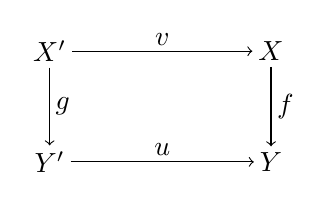
\begin{tikzpicture}[x=1em,y=1em,every node/.style={inner sep=2pt}]
  \node (xprime) at (0,4) {$X'$};
  \node (x) at (8,4) {$X$};
  \node (yprime) at (0,0) {$Y'$};
  \node (y) at (8,0) {$Y$};
  \draw[->] (xprime)--node[above] {$v$} (x);
  \draw[->] (xprime)--node[right] {$g$} (yprime);
  \draw[->] (x)--node[right] {$f$} (y);
  \draw[->] (yprime)--node[above] {$u$} (y);
\end{tikzpicture}\par
}
\smallskip
\emph{Then for all $i\ge0$ there are natural isomorphisms}
\[
u^*R^if_*(\mathcal F)\cong R^ig_*(v^*\mathcal F).
\]

\smallskip
\noindent\textsc{Proof.} The question is local on $Y$ and on $Y'$, so we may assume they are both affine, say $Y=\operatorname{Spec} A$ and $Y'=\operatorname{Spec} A'$. Then by (\Goto{result-III-8.5}{8.5}) what we have to show is that
\[
H^i(X,\mathcal F)\otimes_A A'\cong H^i(X',\mathcal F').
\]
Since $X$ is separated and noetherian, and $\mathcal F$ is quasi-coherent, we can calculate $H^i(X,\mathcal F)$ by \v{C}ech cohomology with respect to an open affine cover $\mathfrak U$ of $X$ (\Goto{result-III-4.5}{4.5}). On the other hand, $\{v^{-1}(U)\mid U\in\mathfrak U\}$ forms an open affine cover $\mathfrak U'$ of $X'$, and clearly the \v{C}ech complex $C^\bullet(\mathfrak U',v^*\mathcal F)$ is just $C^\bullet(\mathfrak U,\mathcal F)\otimes_A A'$. Since $A'$ is flat over $A$, the functor $\cdot\otimes_A A'$ commutes with taking cohomology groups of the \v{C}ech complex, so we get our result. Note that $g$ is also separated and of finite type by base extension, so $X'$ is also noetherian and separated, allowing us to apply (\Goto{result-III-4.5}{4.5}) on $X'$.

\smallskip
\noindent\hypertarget{result-III-9.3.1}{}\textbf{Remark 9.3.1.} Even if $u$ is not flat, this proof shows that there is a natural map $u^*R^if_*(\mathcal F)\to R^ig_*(v^*\mathcal F)$.

\medskip
\noindent\hypertarget{result-III-9.4}{}\textbf{Corollary 9.4.} \emph{Let $f\colon X\to Y$ and $\mathcal F$ be as in (\Goto{result-III-9.3}{9.3}), and assume $Y$ affine. For any point $y\in Y$, let $X_y$ be the fibre over $y$, and let $\mathcal F_y$ be the induced sheaf. On the other hand, let $k(y)$ denote the constant sheaf $k(y)$ on the closed subset $\overline{\{y\}}$ of $Y$. Then for all $i\ge0$ there are natural isomorphisms}
\[
H^i(X_y,\mathcal F_y)\cong H^i(X,\mathcal F\otimes k(y)).
\]

\smallskip
\noindent\textsc{Proof.} First let $Y'\subseteq Y$ be the reduced induced subscheme structure on $\overline{\{y\}}$, and let $X'=X\times_Y Y'$, which is a closed subscheme of $X$. Then both sides of our desired isomorphism depend only on the sheaf $\mathcal F'=\mathcal F\otimes k(y)$ on $X'$. Thus we can replace $X,Y,\mathcal F$ by $X',Y',\mathcal F'$, i.e., we can assume that $Y$ is an integral affine scheme and that $y\in Y$ is its generic point. In that case, $\operatorname{Spec}k(y)\to Y$ is a flat morphism, so we can apply (\Goto{result-III-9.3}{9.3}) and conclude that
\[
H^i(X_y,\mathcal F_y)\cong H^i(X,\mathcal F)\otimes k(y).
\]}
% Contents from body/page-270.tex.
\ChapterSheet{270}{256}{\Goto{p-215}{III\quad Cohomology}}{%
\noindent But after our reduction, $H^i(X,\mathcal F)$ is already a $k(y)$-module, so tensoring with $k(y)$ has no effect, and we obtain the desired result. (This result is used in \Goto{sec-III-12}{\S12}.)

\medskip
\noindent\emph{Flat Families}\par
\smallskip
For many reasons it is important to have a good notion of an algebraic family of varieties or schemes. The most naive definition would be just to take the fibres of a morphism. To get a good notion, however, we should require that certain numerical invariants remain constant in a family, such as the dimension of the fibres. \EditionText{For the projective algebraic families of normal varieties defined below, (\Goto{result-III-9.13}{9.13}) shows that the arithmetic genus is constant.}

\EditionText{For general families of schemes, we impose flatness. A \emph{flat family} of schemes consists of the fibres of a flat morphism.} Why the algebraic condition of flatness on the structure sheaves should give a good definition of a family is something of a mystery. But at least we will justify this choice by showing that flat families have many good properties, and by giving necessary and sufficient conditions for flatness in some special cases. In particular, we will show that a family of closed subschemes of projective space (over an integral scheme) is flat if and only if the Hilbert polynomials of the fibres are the same.

\medskip
\noindent\hypertarget{result-III-9.5}{}\textbf{Proposition 9.5.} \emph{Let $f\colon X\to Y$ be a flat morphism of schemes of finite type over a field $k$. For any point $x\in X$, let $y=f(x)$. Then}
\[
\dim_x(X_y)=\dim_x X-\dim_y Y.
\]
\emph{Here for any scheme $X$ and any point $x\in X$, by $\dim_x X$ we mean the dimension of the local ring $\mathcal O_{x,X}$.}

\smallskip
\noindent\textsc{Proof.} First we make a base change $Y'\to Y$ where $Y'=\operatorname{Spec}\mathcal O_{y,Y}$, and consider the new morphism $f'\colon X'\to Y'$ where $X'=X\times_Y Y'$. Then $f'$ is also flat by (\Goto{result-III-9.2}{9.2}), $x$ lifts to $X'$, and the three numbers in question are the same. Thus we may assume that $y$ is a closed point of $Y$, and $\dim_y Y=\dim Y$.

Now we use induction on $\dim Y$. If $\dim Y=0$, then $X_y$ is defined by a nilpotent ideal in $X$, so we have $\dim_x(X_y)=\dim_x X$, and $\dim_y Y=0$.

If $\dim Y>0$, we make a base extension to $Y_{\mathrm{red}}$. Nothing changes, so we may assume that $Y$ is reduced. Then we can find an element $t\in\mathfrak m_y\subseteq\mathcal O_{y,Y}$ such that $t$ is not a zero divisor. Let $Y'=\operatorname{Spec}\mathcal O_{y,Y}/(t)$, and make the base extension $Y'\to Y$. Then $\dim Y'=\dim Y-1$ by (I, \Goto{result-I-1.8A}{1.8A}) and (I, \Goto{result-I-1.11A}{1.11A}). Since $f$ is flat, $f^\#t\in\mathfrak m_x$ is also not a zero divisor. So for the same reason, $\dim_x X'=\dim_x X-1$. Of course the fibre $X_y$ does not change under base extension, so we have only to prove our formula for $f'\colon X'\to Y'$. But this follows from the induction hypothesis, so we are done.}
% Contents from body/page-271.tex.
\ChapterSheet{271}{257}{\Goto{sec-III-9}{9\quad Flat Morphisms}}{%
\noindent\hypertarget{result-III-9.6}{}\textbf{Corollary 9.6.} \emph{Let $f\colon X\to Y$ be a flat morphism of schemes of finite type over a field $k$, and assume that $Y$ is irreducible. Then the following conditions are equivalent:}

\noindent\hspace*{1.7em}\hypertarget{result-III-9.6-i}{}(i) \emph{every irreducible component of $X$ has dimension equal to $\dim Y+n$;}

\noindent\hangindent=3em\hspace*{1.7em}\hypertarget{result-III-9.6-ii}{}(ii) \emph{for any point $y\in Y$ (closed or not), every irreducible component of the fibre $X_y$ has dimension $n$.}

\medskip
\noindent\textsc{Proof.}

\Goto{result-III-9.6-i}{(i)} $\Rightarrow$ \Goto{result-III-9.6-ii}{(ii)}. Given $y\in Y$, let $Z\subseteq X_y$ be an irreducible component, and let $x\in Z$ be a closed point, which is not in any other irreducible component of $X_y$. Applying (\Goto{result-III-9.5}{9.5}) we have
\[
\dim_x Z=\dim_x X-\dim_y Y.
\]
Now $\dim_x Z=\dim Z$ since $x$ is a closed point (II, Ex.~\Goto{ex-II-3.20}{3.20}). On the other hand, since $Y$ is irreducible and $X$ is equidimensional, and both are of finite type over $k$, we have (II, Ex.~\Goto{ex-II-3.20}{3.20})
\[
\begin{aligned}
\dim_x X&=\dim X-\dim\overline{\{x\}},\\
\dim_y Y&=\dim Y-\dim\overline{\{y\}}.
\end{aligned}
\]
Finally, since $x$ is a closed point of the fibre $X_y$, $k(x)$ is a finite algebraic extension of $k(y)$ and so
\[
\dim\overline{\{x\}}=\dim\overline{\{y\}}.
\]
Combining all these, and using \Goto{result-III-9.6-i}{(i)} we find $\dim Z=n$.

\Goto{result-III-9.6-ii}{(ii)} $\Rightarrow$ \Goto{result-III-9.6-i}{(i)}. This time let $Z$ be an irreducible component of $X$, and let $x\in Z$ be a closed point which is not contained in any other irreducible component of $X$. Then applying (\Goto{result-III-9.5}{9.5}), we have
\[
\dim_x(X_y)=\dim_x X-\dim_y Y.
\]
But $\dim_x(X_y)=n$ by \Goto{result-III-9.6-ii}{(ii)}, $\dim_x X=\dim Z$, and $\dim_y Y=\dim Y$, since $y=f(x)$ must be a closed point of $Y$. Thus
\[
\dim Z=\dim Y+n
\]
as required.

\medskip
\noindent\hypertarget{err-4}{}\textbf{Definition.} A point $x$ of a \EditionText{locally noetherian }scheme $X$ is an \emph{associated point} of $X$ if the maximal ideal $\mathfrak m_x$ is an associated prime of $0$ in the local ring $\mathcal O_{x,X}$, or in other words, if every element of $\mathfrak m_x$ is a zero divisor.

\medskip
\noindent\hypertarget{result-III-9.7}{}\textbf{Proposition 9.7.} \emph{Let $f\colon X\to Y$ be a morphism of schemes, with \EditionText{$X$ locally noetherian and }$Y$ integral and regular of dimension $1$. Then $f$ is flat if and only if every associated point $x\in X$ maps to the generic point of $Y$. In particular, if $X$ is reduced, this says that every irreducible component of $X$ dominates $Y$.}}
% Contents from body/page-272.tex.
\ChapterSheet[10.55]{272}{258}{\Goto{p-215}{III\quad Cohomology}}{%
\noindent\textsc{Proof.} First suppose that $f$ is flat, and let $x\in X$ be a point whose image $y=f(x)$ is a closed point of $Y$. Then $\mathcal O_{y,Y}$ is a discrete valuation ring. Let $t\in\mathfrak m_y-\mathfrak m_y^2$ be a uniformizing parameter. Then $t$ is not a zero divisor in $\mathcal O_{y,Y}$. Since $f$ is flat, $f^\#t\in\mathfrak m_x$ is not a zero divisor, so $x$ is not an associated point of $X$.

Conversely, suppose that every associated point of $X$ maps to the generic point of $Y$. To show $f$ is flat, we must show that for any $x\in X$, letting $y=f(x)$, the local ring $\mathcal O_{x,X}$ is flat over $\mathcal O_{y,Y}$. If $y$ is the generic point, $\mathcal O_{y,Y}$ is a field, so there is nothing to prove. If $y$ is a closed point, $\mathcal O_{y,Y}$ is a discrete valuation ring, so by (\Goto{result-III-9.1.3}{9.1.3}) we must show that $\mathcal O_{x,X}$ is a torsion-free module. If it is not, then $f^\#t$ must be a zero divisor in $\mathcal O_x$, where $t$ is a uniformizing parameter of $\mathcal O_{y,Y}$. Therefore $f^\#t$ is contained in some associated prime ideal $\mathfrak p$ of $(0)$ in $\mathcal O_x$ (Matsumura \Goto{bib-479-17}{[2, Cor.~2, p.~50]}). Then $\mathfrak p$ determines a point $x'\in X$, which is an associated point of $X$, and whose image by $f$ is $y$, which is a contradiction.

Finally, note that if $X$ is reduced, its associated points are just the generic points of its irreducible components, so our condition says that each irreducible component of $X$ dominates $Y$.

\smallskip
\noindent\hypertarget{result-III-9.7.1}{}\textbf{Example 9.7.1.} Let $Y$ be a curve with a node, and let $f\colon X\to Y$ be the map of its normalization to it. Then $f$ is not flat. For if it were, then $f_*\mathcal O_X$ would be a flat sheaf of $\mathcal O_Y$-modules. Since it is coherent, it would be locally free by (\Goto{result-III-9.2-e}{9.2e}). And finally, since its rank is $1$, it would be an invertible sheaf on $Y$. But there are two points $P_1,P_2$ of $X$ going to the node $Q$ of $Y$, so $(f_*\mathcal O_X)_Q$ needs two generators as an $\mathcal O_Y$-module, hence it cannot be locally free.

\smallskip
\noindent\hypertarget{result-III-9.7.2}{}\textbf{Example 9.7.2.} The result of (\Goto{result-III-9.7}{9.7}) also fails if $Y$ is regular of dimension $>1$. For example, let $Y=\AffSpace{2}$, and let $X$ be obtained by blowing up a point. Then $X$ and $Y$ are both nonsingular, and $X$ dominates $Y$, but $f$ is not flat, because the dimension of the fibre over the blown-up point is too big (\Goto{result-III-9.5}{9.5}).

\smallskip
\noindent\hypertarget{result-III-9.8}{}\textbf{Proposition 9.8.} \emph{Let $Y$ be a regular, integral scheme of dimension $1$, let $P\in Y$ be a closed point, and let $X\subseteq\mathbf P^n_{Y-P}$ be a closed subscheme which is flat over $Y-P$. Then there exists a unique closed subscheme $\overline X\subseteq\mathbf P^n_Y$, flat over $Y$, whose restriction to $\mathbf P^n_{Y-P}$ is $X$.}

\smallskip
\noindent\textsc{Proof.} \EditionText{For each affine $\operatorname{Spec} A\subseteq Y$, write $K=\operatorname{Frac} A$. On each standard affine chart $\operatorname{Spec} B$ of $\mathbf P^n_A$, let $J_K\subseteq B\otimes_A K$ be the generic-fibre ideal and take $J$ to be its inverse image in $B$. Contraction commutes with localization, so these ideals glue. The quotient $B/J$ embeds in $(B\otimes_A K)/J_K$ and is torsion-free over $A$. Its localizations are flat over the corresponding base local rings, which are fields or discrete valuation rings. Conversely, every flat quotient over such a chart is torsion-free over $A$, so its ideal is the contraction of its generic-fibre ideal. This identifies the restriction over $Y-P$ with $X$ and proves uniqueness. The construction gives the scheme-theoretic closure.}

\smallskip
\noindent\hypertarget{result-III-9.8.1}{}\textbf{Remark 9.8.1.} This proposition says that we can \textquotedblleft{}pass to the limit,\textquotedblright{} when we have a flat family of closed subschemes of $\mathbf P^n$ over a punctured curve. Hence \EditionText{it implies that the Hilbert scheme for a fixed Hilbert polynomial is proper.} The Hilbert scheme is a}
% Contents from body/page-273.tex.
\ChapterSheet[10.8]{273}{259}{\Goto{sec-III-9}{9\quad Flat Morphisms}}{%
\noindent scheme $H$ which parametrizes all closed subschemes of $\mathbf P_k^n$. It has the property that to give a closed subscheme $X\subseteq\mathbf P_T^n$, flat over $T$, for any scheme $T$, is equivalent to giving a morphism $\varphi\colon T\to H$. Here, naturally, for any $t\in T$, $\varphi(t)$ is the point of $H$ corresponding to the fibre $X_t\subseteq\mathbf P_{k(t)}^n$.

Now once one knows that the Hilbert scheme exists (see Grothendieck \Goto{bib-476-5}{[5, exp.~221]}) then the question of \EditionText{the properness of each fixed-polynomial part} can be decided using the valuative criterion of properness (II, \Goto{result-II-4.7}{4.7}). And the result just proved is the essential point needed to show that each connected component of $H$ is proper over $k$.

\medskip
\noindent\hypertarget{result-III-9.8.2}{}\textbf{Example 9.8.2.} Even though the dimension of the fibres is constant in a \EditionText{flat family of closed subschemes of projective space over a connected noetherian base (\Goto{result-III-9.10}{9.10})}, we cannot expect properties such as \textquotedblleft{}irreducible\textquotedblright{} or \textquotedblleft{}reduced\textquotedblright{} to be preserved in a flat family. Take for example, the families given in (II, \Goto{result-II-3.3.1}{3.3.1}) and (II, \Goto{result-II-3.3.2}{3.3.2}). In each case the total space $X$ is integral, the base $Y$ is a nonsingular curve and the morphism $f\colon X\to Y$ is surjective, so the family is flat. Also most fibres are integral in both families. However, the special fibre in one is a doubled line (not reduced), and the special fibre in the other is two lines (not irreducible).

\medskip
\noindent\hypertarget{result-III-9.8.3}{}\textbf{Example 9.8.3} (Projection from a Point). We get some new insight into the geometric process of projection from a point (I, Ex.~\Goto{ex-I-3.14}{3.14}) using (\Goto{result-III-9.8}{9.8}). Let $P=(0,0,\ldots,0,1)\in\mathbf P^{n+1}$, and consider the projection $\varphi\colon\mathbf P^{n+1}-\{P\}\to\mathbf P^n$, which is defined by $(x_0,\ldots,x_{n+1})\mapsto(x_0,\ldots,x_n)$. For each $a\in k$, $a\ne0$, consider the automorphism $\sigma_a$ of $\mathbf P^{n+1}$ defined by $(x_0,\ldots,x_{n+1})\mapsto(x_0,\ldots,x_n,ax_{n+1})$. Now let $X_1$ be a closed subscheme of $\mathbf P^{n+1}$, not containing $P$. For each $a\ne0$, let $X_a=\sigma_a(X_1)$. Then the $X_a$ form a flat family parametrized by $\AffSpace{1}-\{0\}$. \EditionText{The map $(x,a)\mapsto(\sigma_a(x),a)$ is an isomorphism over the punctured line from $X_1\times(\AffSpace{1}-\{0\})$ to the family, with inverse induced by $\sigma_{a^{-1}}$. Thus the family is flat.}

Now according to (\Goto{result-III-9.8}{9.8}) this family extends uniquely to a flat family defined over all of $\AffSpace{1}$\EditionText{. Since $X_1$ avoids $P$, the same homogeneous coordinate formula extends at $a=0$ with value $\varphi(x)$. This gives a proper morphism over $\AffSpace{1}$ from $X_1\times\AffSpace{1}$ into the ambient projective family. Its image is closed and is the closure of its image over the punctured line. Hence the support of $X_0$ is $\varphi(X_1)$.} Thus we see that there is a flat family over $\AffSpace{1}$, whose fibres for all $a\ne0$ are isomorphic to $X_1$, and whose fibre at $0$ is some scheme with the same underlying space as $\varphi(X_1)$.

\medskip
\noindent\hypertarget{result-III-9.8.4}{}\textbf{Example 9.8.4.} \EditionText{Assume that $\operatorname{char}k\ne2$. }We will now calculate the flat family just described in the special case where $X_1$ is a twisted cubic curve in $\mathbf P^3$, $\varphi$ is a projection to $\mathbf P^2$, and $\varphi(X_1)$ is a nodal cubic curve in $\mathbf P^2$. The remarkable result of this calculation is that the special fibre $X_0$ of our flat family consists of the curve $\varphi(X_1)$ together with some nilpotent elements at the double point! We say that $X_0$ is a scheme with an \emph{embedded point}. It seems as if the scheme $X_0$ is retaining the information that it is the limit of a family of space curves, by having these nilpotent elements which point out of the plane. In particular, $X_0$ is not a closed subscheme of $\mathbf P^2$ (Fig.~\Goto{fig-book-11}{11}).}
% Contents from body/page-274.tex.
\ChapterSheet[10.9]{274}{260}{\Goto{p-215}{III\quad Cohomology}}{%
{\centering
\hypertarget{fig-book-11}{}%
\resizebox{.69\linewidth}{!}{%
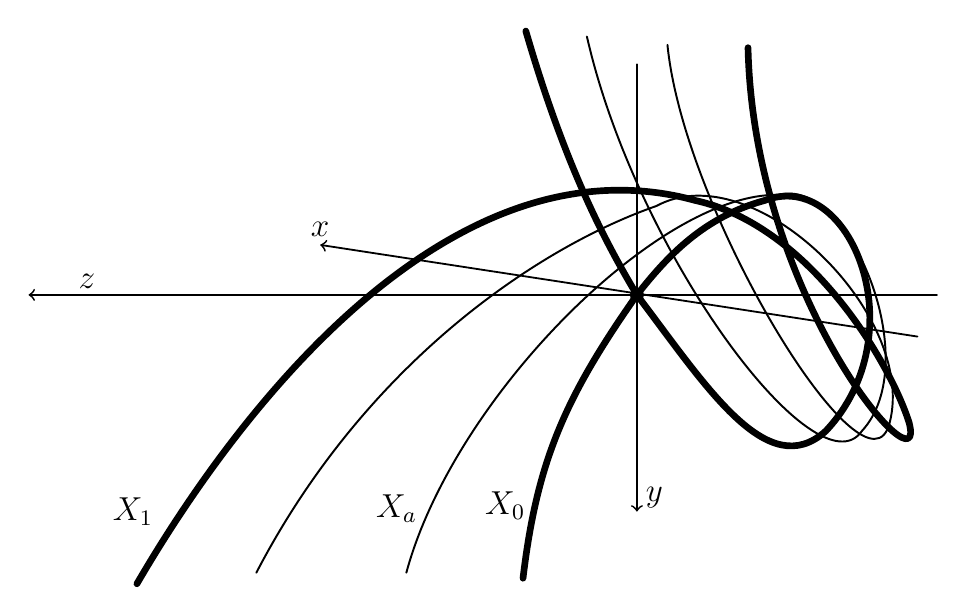
\begin{tikzpicture}[x=1bp,y=-1bp,line cap=round,line join=round,
  fibre/.style={line width=.7bp}, end fibre/.style={line width=2.4bp},
  every node/.style={font=\large,inner sep=2bp}]
  % The three projected coordinate axes.
  \draw[->,line width=.65bp] (328,97) -- (1,97);
  \draw[->,line width=.65bp] (321,112) -- (106,79);
  \draw[->,line width=.65bp] (220,14) -- (220,175);
  % The four drawn fibres, from the space cubic to the planar limit.
  \draw[end fibre] (260,8) .. controls (262,99) and (325,170) .. (318,143)
    .. controls (311,121) and (282,72) .. (241,63)
    .. controls (157,40) and (82,129) .. (40,201);
  \draw[fibre] (231,7) .. controls (237,68) and (303,175) .. (311,143)
    .. controls (321,104) and (262,46) .. (227,65)
    .. controls (184,80) and (122,122) .. (83,197);
  \draw[fibre] (202,4) .. controls (220,83) and (285,169) .. (301,146)
    .. controls (324,121) and (296,54) .. (271,61)
    .. controls (228,60) and (154,134) .. (137,197);
  \draw[end fibre] (180,2) .. controls (194,50) and (208,77) .. (220,97)
    .. controls (245,130) and (267,165) .. (288,146)
    .. controls (321,111) and (297,51) .. (266,63)
    .. controls (244,69) and (231,83) .. (220,97)
    .. controls (194,134) and (184,157) .. (179,199);
  \fill (220,97) circle[radius=2.5bp];
  \node[above] at (22,97) {$z$};
  \node[above] at (106,78) {$x$};
  \node[right] at (221,170) {$y$};
  \node[left] at (48,175) {$X_1$};
  \node[left] at (143,174) {$X_a$};
  \node[left] at (182,173) {$X_0$};
\end{tikzpicture}}\par
\smallskip
\small\textbf{Figure 11.}\enspace A flat family of subschemes of $\mathbf P^3$.\par
}
\medskip
Now for the calculation. We are just interested in what happens near the double point, so we will use affine coordinates $x,y$ in $\AffSpace{2}$ and $x,y,z$ in $\AffSpace{3}$. Let $X_1$ be given by the parametric equations
\[
\begin{cases}
x=t^2-1\\
y=t^3-t\\
z=t.
\end{cases}
\]
Then since $t=z$, $t^2=x+1$, $t^3=y+z$, we recognize this as a twisted cubic curve in $\AffSpace{3}$ (I, Ex.~\Goto{ex-I-1.2}{1.2}).

Now for any $a\ne0$, the scheme $X_a$ is given by
\[
\begin{cases}
x=t^2-1\\
y=t^3-t\\
z=at.
\end{cases}
\]
To get the ideal $I\subseteq k[a,x,y,z]$ of the total family $\overline X$ extended over all of $\AffSpace{1}$, we eliminate $t$ from the parametric equations, and make sure $a$ is not a zero divisor in $k[a,x,y,z]/I$, so that $\overline X$ will be flat. We find
\[
I=(a^2(x+1)-z^2,\,ax(x+1)-yz,\,xz-ay,\,y^2-x^2(x+1)).
\]
From this, setting $a=0$, we obtain the ideal $I_0\subseteq k[x,y,z]$ of $X_0$, which is
\[
I_0=(z^2,yz,xz,y^2-x^2(x+1)).
\]
So we see that $X_0$ is a scheme with support equal to the nodal cubic curve $y^2=x^2(x+1)$. At any point where $x\ne0$, we get $z$ in the ideal, so $X_0$ is reduced there. But in the local ring at the node $(0,0,0)$, we have the element $z$ with $z^2=0$, a nonzero nilpotent element.

So here we have an example of a flat family of curves, whose general member is nonsingular, but whose special member is singular, with an embedded point. See also (\Goto{result-III-9.10.1}{9.10.1}) and (IV, Ex.~\Goto{ex-IV-3.5}{3.5}).}
% Contents from body/page-275.tex.
\ChapterSheet{275}{261}{\Goto{sec-III-9}{9\quad Flat Morphisms}}{%
\noindent\hypertarget{result-III-9.8.5}{}\textbf{Example 9.8.5} (Algebraic Families of Divisors). Let $X$ be a scheme of finite type over an algebraically closed field $k$, let $T$ be a nonsingular curve over $k$, and let $D$ be an effective Cartier divisor on $X\times T$ (II, \Goto{sec-II-6}{\S6}). Then we can think of $D$ as a closed subscheme of $X\times T$, which is locally described on a small open set $U$ as the zeros of a single element $f\in\Gamma(U,\mathcal O_U)$ such that $f$ is not a zero divisor. For any closed point $t\in T$, let $X_t\ (\cong X)$ be the fibre of $X\times T$ over $t$. We say that the intersection divisor $D_t=D\cdot X_t$ is \emph{defined} if at every point of $X_t$, the image $\bar f\in\Gamma(U\cap X_t,\mathcal O_{X_t})$ of a local equation $f$ of $D$ is not a zero divisor. In that case the covering $\{U\cap X_t\}$ and the elements $\bar f$ define a Cartier divisor $D_t$ on $X_t$. If $D_t$ is defined for all $t$, we say that the divisors $\{D_t\mid t\in T\}$ form an \emph{algebraic family of divisors on $X$ parametrized by $T$}.

This definition, which is natural in the context of Cartier divisors, is connected with flatness in the following way: the original Cartier divisor $D$, considered as a scheme over $T$, is flat over $T$ if and only if $D_t=D\cdot X_t$ is defined for each \EditionText{closed point $t\in T$}. \EditionText{At points of $D$ over the generic point of $T$, flatness is automatic. For $x\in D$ over a closed point $t=p_2(x)$, take $A=\mathcal O_{x,X\times T}$, a local equation $f\in A$ of $D$, and a uniformizing parameter $u\in\mathcal O_{t,T}$.} Then $D\cdot X_t$ is defined at $x$ if and only if $\bar f\in A/uA$ is not a zero divisor. Since $u$ is automatically not a zero divisor in $A$, this is equivalent to saying that $(u,f)$ is a regular sequence (II, \Goto{sec-II-8}{\S8}) in $A$. On the other hand, $D$ is flat over $T$ at $x$ if and only if $\mathcal O_{x,D}$ is flat over $\mathcal O_{t,T}$. By (\Goto{result-III-9.1.3}{9.1.3}) this is equivalent to $\mathcal O_{x,D}$ being torsion-free, i.e., $u$ not being a zero divisor in $\mathcal O_{x,D}$. But $\mathcal O_{x,D}\cong A/fA$, so this says that $(f,u)$ is a regular sequence in $A$. Since the property of being a regular sequence is independent of the order of the sequence (Matsumura \Goto{bib-479-17}{[2, Th.~28, p.~102]}), the two conditions are equivalent.

\medskip
\noindent\hypertarget{result-III-9.9}{}\textbf{Theorem 9.9.} \emph{Let $T$ be an integral noetherian scheme. Let $X\subseteq\mathbf P_T^n$ be a closed subscheme. For each point $t\in T$, we consider the Hilbert polynomial $P_t\in\mathbb Q[z]$ of the fibre $X_t$ considered as a closed subscheme of $\mathbf P_{k(t)}^n$. Then $X$ is flat over $T$ if and only if the Hilbert polynomial $P_t$ is independent of $t$.}

\smallskip
\noindent\textsc{Proof.} Recall that the Hilbert polynomial was defined in (I, \Goto{sec-I-7}{\S7}), and computed another way in (Ex.~\Goto{ex-III-5.2}{5.2}). We will use the defining property that
\[
P_t(m)=\dim_{k(t)}H^0(X_t,\mathcal O_{X_t}(m))
\]
for all $m\gg0$.

First we generalize, replacing $\mathcal O_X$ by any coherent sheaf $\mathcal F$ on $\mathbf P_T^n$, and using the Hilbert polynomial of $\mathcal F_t$. Thus we may assume $X=\mathbf P_T^n$. Second, the question is local on $T$. In fact, by comparing any point to the generic point, we see that it is sufficient to consider the case $T=\operatorname{Spec} A$, with $A$ a local noetherian ring.

So now let $T=\operatorname{Spec} A$ with $A$ a local noetherian domain, let $X=\mathbf P_T^n$, and let $\mathcal F$ be a coherent sheaf on $X$. We will show that the following conditions are equivalent:

\noindent\hypertarget{result-III-9.9-i}{}(i) $\mathcal F$ is flat over $T$;

\noindent\hypertarget{result-III-9.9-ii}{}(ii) $H^0(X,\mathcal F(m))$ is a free $A$-module of finite rank, for all $m\gg0$;}
% Contents from body/page-276.tex.
\ChapterSheet[10.8]{276}{262}{\Goto{p-215}{III\quad Cohomology}}{%
\noindent\hangindent=3em\hspace*{1.7em}\hypertarget{result-III-9.9-iii}{}(iii) the Hilbert polynomial $P_t$ of $\mathcal F_t$ on $X_t=\mathbf P_{k(t)}^n$ is independent of $t$, for any $t\in T$.

\Goto{result-III-9.9-i}{(i)} $\Rightarrow$ \Goto{result-III-9.9-ii}{(ii)}. We compute $H^i(X,\mathcal F(m))$ by \v{C}ech cohomology using the standard open affine cover $\mathfrak U$ of $X$. Then
\[
H^i(X,\mathcal F(m))=h^i(C^\bullet(\mathfrak U,\mathcal F(m))).
\]
Since $\mathcal F$ is flat, each term $C^i(\mathfrak U,\mathcal F(m))$ of the \v{C}ech complex is a flat $A$-module. On the other hand, if $m\gg0$, then $H^i(X,\mathcal F(m))=0$ for $i>0$, by (\Goto{result-III-5.2}{5.2}). Thus the complex $C^\bullet(\mathfrak U,\mathcal F(m))$ is a resolution of the $A$-module $H^0(X,\mathcal F(m))$: we have an exact sequence
{\small
\[
0\to H^0(X,\mathcal F(m))\to C^0(\mathfrak U,\mathcal F(m))\to C^1(\mathfrak U,\mathcal F(m))\to\cdots\to C^n(\mathfrak U,\mathcal F(m))\to0.
\]}
Splitting this into short exact sequences, using (\Goto{result-III-9.1A}{9.1Ae}) and the fact that the $C^i$ are all flat, we conclude that $H^0(X,\mathcal F(m))$ is a flat $A$-module. But it is also finitely generated (\Goto{result-III-5.2}{5.2}), and hence free of finite rank by (\Goto{result-III-9.1A}{9.1Af}).

\Goto{result-III-9.9-ii}{(ii)} $\Rightarrow$ \Goto{result-III-9.9-i}{(i)}. Let $S=A[x_0,\ldots,x_n]$, and let $M$ be the graded $S$-module
\[
M=\bigoplus_{m\ge m_0}H^0(X,\mathcal F(m)),
\]
where $m_0$ is chosen large enough so that the $H^0(X,\mathcal F(m))$ are all free for $m\ge m_0$. Then $\mathcal F=\widetilde M$ by (II, \Goto{result-II-5.15}{5.15}). Note that $M$ is the same as $\Gamma_*(\mathcal F)$ in degrees $m\ge m_0$, so $\widetilde M=\Gamma_*(\mathcal F)^\sim$. Since $M$ is a free (and hence flat) $A$-module, we see that $\mathcal F$ is flat over $A$ (\Goto{result-III-9.1.1}{9.1.1}).

\Goto{result-III-9.9-ii}{(ii)} $\Rightarrow$ \Goto{result-III-9.9-iii}{(iii)}. It will be enough to show that
\[
P_t(m)=\operatorname{rank}_A H^0(X,\mathcal F(m))
\]
for $m\gg0$. To prove this we will show, for any $t\in T$, that
\[
H^0(X_t,\mathcal F_t(m))\cong H^0(X,\mathcal F(m))\otimes_A k(t)
\]
for all $m\gg0$.

First we let $T'=\operatorname{Spec} A_{\mathfrak p}$, where $\mathfrak p$ is the prime ideal corresponding to $t$, and we make the flat base extension $T'\to T$. Thus by (\Goto{result-III-9.3}{9.3}) we reduce to the case where $t$ is the closed point of $T$. Denote the closed fibre $X_t$ by $X_0$, $\mathcal F_t$ by $\mathcal F_0$, and $k(t)$ by $k$. Take a presentation of $k$ over $A$,
\[
A^q\longrightarrow A\longrightarrow k\longrightarrow0.
\]
Then we get an exact sequence of sheaves on $X$,
\[
\mathcal F^q\longrightarrow\mathcal F\longrightarrow\mathcal F_0\longrightarrow0.
\]
Now by (Ex.~\Goto{ex-III-5.10}{5.10}) for $m\gg0$ we get an exact sequence
\[
H^0(X,\mathcal F(m)^q)\longrightarrow H^0(X,\mathcal F(m))\longrightarrow H^0(X_0,\mathcal F_0(m))\longrightarrow0.
\]
On the other hand, we can tensor the sequence $A^q\to A\to k\to0$ with $H^0(X,\mathcal F(m))$. Comparing, we deduce that
\[
H^0(X_0,\mathcal F_0(m))\cong H^0(X,\mathcal F(m))\otimes_A k
\]
for all $m\gg0$, as required.}
% Contents from body/page-277.tex.
\ChapterSheet{277}{263}{\Goto{sec-III-9}{9\quad Flat Morphisms}}{%
\noindent\Goto{result-III-9.9-iii}{(iii)} $\Rightarrow$ \Goto{result-III-9.9-ii}{(ii)}. According to (II, \Goto{result-II-8.9}{8.9}) we can check the freeness of $H^0(X,\mathcal F(m))$ by comparing its rank at the generic point and the closed point of $T$. Hence the argument of \Goto{result-III-9.9-ii}{(ii)} $\Rightarrow$ \Goto{result-III-9.9-iii}{(iii)} above is reversible.

\medskip
\noindent\hypertarget{result-III-9.10}{}\textbf{Corollary 9.10.} \emph{Let $T$ be a connected noetherian scheme, and let $X\subseteq\mathbf P^n_T$ be a closed subscheme which is flat over $T$. For any $t\in T$, let $X_t$ be the fibre, considered as a closed subscheme of $\mathbf P_{k(t)}^n$. Then the dimension of $X_t$, the degree of $X_t$, and the arithmetic genus of $X_t$ are all independent of $t$.}

\smallskip
\noindent\textsc{Proof.} By base extension to the irreducible components of $T$ with their reduced induced structure, we reduce to the case $T$ integral. Now the result follows from the theorem and the facts (I, \Goto{sec-I-7}{\S7}) and (Ex.~\Goto{ex-III-5.3}{5.3}) that
\[
\begin{aligned}
\dim X_t&=\deg P_t,\\
\deg X_t&=(r!)\cdot(\text{leading coefficient of }P_t),
\end{aligned}
\]
where $r=\dim\EditionText{X_t}$, and
\[
p_a(X_t)=(-1)^r(P_t(0)-1).
\]

\medskip
\noindent\textbf{Definition.} Let $k$ be an algebraically closed field, let $f\colon X\to T$ be a surjective map of varieties over $k$, and assume that for each closed point $t\in T$, we have

\noindent\hspace*{1em}(1) $f^{-1}(t)$ is irreducible of dimension equal to $\dim X-\dim T$, and

\noindent\hangindent=2.4em\hspace*{1em}(2) if $\mathfrak m_t\subseteq\mathcal O_{t,T}$ is the maximal ideal, and if $\zeta\in f^{-1}(t)$ is the generic point, then $f^\#\mathfrak m_t$ generates the maximal ideal $\mathfrak m_\zeta\subseteq\mathcal O_{\zeta,X}$.

Under these circumstances, we let $X_{(t)}$ be the variety $f^{-1}(t)$ (with the reduced induced structure) and we say that the $X_{(t)}$ form an \emph{algebraic family of varieties}, parametrized by $T$. The second condition is necessary to be sure that $X_{(t)}$ occurs with \textquotedblleft{}multiplicity one\textquotedblright{} in the family. It is equivalent to saying that the scheme-theoretic fibre $X_t$ is reduced at its generic point.

\medskip
\noindent\hypertarget{result-III-9.10.1}{}\textbf{Example 9.10.1.} In the flat family of (\Goto{result-III-9.8.4}{9.8.4})\EditionText{, with $\operatorname{char}k\ne2$}, if we take the fibres with their reduced induced structures, we get an algebraic family of varieties $X_{(t)}$ parametrized by $\AffSpace{1}$. For $t\ne0$ it is a nonsingular rational curve, and for $t=0$ it is the plane nodal cubic curve. Note that the arithmetic genus is not constant in this family: $p_a(X_{(t)})=0$ for $t\ne0$ and $p_a(X_{(0)})=1$. This accounts for the appearance of nilpotent elements in the scheme-theoretic fibre $X_0$, since in a flat family of schemes $p_a$ is constant by (\Goto{result-III-9.10}{9.10}). The embedded point at $0$ alters the constant term of the Hilbert polynomial so that we get $p_a(X_0)=0$.

\medskip
\noindent\hypertarget{result-III-9.11}{}\textbf{Theorem 9.11.} \emph{Let $X_{(t)}$ be an algebraic family of normal varieties parametrized by a nonsingular curve $T$ over an algebraically closed field $k$. Then $X_{(t)}$ is a flat family of schemes.}}
% Contents from body/page-278.tex.
\ChapterSheet[10.65]{278}{264}{\Goto{p-215}{III\quad Cohomology}}{%
\noindent\textsc{Proof.} Let $f\colon X\to T$ be the defining morphism of the family. Then $f$ is a flat morphism by (\Goto{result-III-9.7}{9.7}). So we have only to show that for each closed point $t\in T$, the scheme-theoretic fibre $X_t$ coincides with the variety $X_{(t)}$. In other words, we must show that $X_t$ is reduced. For any point $x\in X$, let $A=\mathcal O_{x,X}$ be its local ring, let $f(x)=t$, and denote also by $t$ a uniformizing parameter in the local ring $\mathcal O_{t,T}$. Then $A/tA$ is the local ring of $x$ on $X_t$. By hypothesis $X_t$ is irreducible, so $t$ has a unique minimal prime ideal $\mathfrak p$ in $A$. Furthermore, $t$ generates the maximal ideal of the local ring of the generic point of $X_t$ on $X$, which says that $t$ generates the maximal ideal of $A_{\mathfrak p}$. Finally, the local ring of $x$ on $X_{(t)}$ is $A/\mathfrak p$, so our hypothesis says that $A/\mathfrak p$ is normal. Now our result is a consequence of the following lemma, which tells us that $\mathfrak p=tA$, so $X_{(t)}=X_t$.

\medskip
\noindent\hypertarget{result-III-9.12}{}\textbf{Lemma 9.12} (Lemma of Hironaka \Goto{bib-477-12-item-1}{[1]}). \emph{Let $A$ be a local noetherian domain, which is a localization of an algebra of finite type over a field $k$. Let $t\in A$, and assume}

\noindent\hspace*{1em}(1) \emph{$tA$ has only one minimal associated prime ideal $\mathfrak p$,}

\noindent\hspace*{1em}(2) \emph{$t$ generates the maximal ideal of $A_{\mathfrak p}$,}

\noindent\hspace*{1em}(3) \emph{$A/\mathfrak p$ is normal.}

\noindent\emph{Then $\mathfrak p=tA$ and $A$ is normal.}

\smallskip
\noindent\textsc{Proof.} \EditionText{If $t=0$, then $\mathfrak p=0$ and (3) gives the result, so assume $t\ne0$. }Let $\widetilde A$ be the normalization of $A$. Then $\widetilde A$ is a finitely generated $A$-module by (I, \Goto{result-I-3.9A}{3.9A}). We will show that the maps
\[
\varphi\colon A/tA\to\widetilde A/t\widetilde A
\]
and
\[
\psi\colon A/tA\to A/\mathfrak p
\]
are both isomorphisms.

First we localize at $\mathfrak p$. Then $\psi$ is an isomorphism by hypothesis. Therefore $A_{\mathfrak p}$ is a discrete valuation ring, hence normal. So $\widetilde A_{\mathfrak p}=A_{\mathfrak p}$, and $\varphi$ is also an isomorphism.

Now suppose that at least one of $\varphi,\psi$ is not an isomorphism. Then, after localizing $A$ at a suitable prime ideal, we may assume that $\varphi$ and $\psi$ are isomorphisms at every localization $A_{\mathfrak q}$ with $\mathfrak q\ne\mathfrak m$, but that at least one of $\varphi,\psi$ is not an isomorphism at $\mathfrak m$. By the previous step, we have $\mathfrak p<\mathfrak m$, so $\dim A\ge2$. \EditionText{Write $B=\widetilde A$. Each maximal ideal $\mathfrak n$ of $B$ above $\mathfrak m$ has height $\dim A$ by the dimension formula, since the fraction fields agree and the residue extension is finite. By normality (II, \Goto{result-II-8.22A}{8.22A}), $\operatorname{depth}B_{\mathfrak n}\ge2$ and $\operatorname{depth}(B_{\mathfrak n}/tB_{\mathfrak n})\ge1$. Thus no associated prime of $B/tB$ lies over $\mathfrak m$. Off $\mathfrak m$ the quotient agrees with $A/\mathfrak p$, so it has a single minimal prime, is generically reduced, and has no embedded associated primes. It is therefore a domain.} Thus we have a natural map $(A/tA)_{\mathrm{red}}\to\widetilde A/t\widetilde A$. \EditionText{By the unique minimal prime in (1), $(A/tA)_{\mathrm{red}}\cong A/\mathfrak p$.} Thus $\widetilde A/t\widetilde A$ is a finitely generated $(A/\mathfrak p)$-module with the same quotient field. Since $A/\mathfrak p$ is normal by hypothesis, we conclude that $\widetilde A/t\widetilde A\cong A/\mathfrak p$. Therefore $\varphi$ is surjective, so we can write $\widetilde A=A+t\widetilde A$. By Nakayama's lemma, this implies that $A=\widetilde A$. Thus $A/tA\cong A/\mathfrak p$ and both $\varphi$ and $\psi$ are isomorphisms. But this is a contradiction, so we conclude that $\varphi$ and $\psi$ were already isomorphisms on the original ring $A$ before localization.}
% Contents from body/page-279.tex.
\ChapterSheet[10.65]{279}{265}{\Goto{sec-III-9}{9\quad Flat Morphisms}}{%
\fontsize{9.5}{10.25}\selectfont%
\setlength{\parskip}{0pt}%
\setlength{\smallskipamount}{1.75pt}%
\setlength{\medskipamount}{3pt}%
\setlength{\abovedisplayskip}{3pt}%
\setlength{\belowdisplayskip}{3pt}%
To conclude, we find that $\mathfrak p=tA$ because $\psi$ is an isomorphism. Since $\varphi$ is an isomorphism, we have $\widetilde A=A+t\widetilde A$, so by Nakayama's lemma as before, we find that $A=\widetilde A$, so $A$ is normal.

\medskip
\noindent\hypertarget{result-III-9.13}{}\textbf{Corollary 9.13} (Igusa \Goto{bib-478-4-item-1}{[1]}). \emph{Let $X_{(t)}$ be an algebraic family of normal varieties in $\mathbf P_k^n$, parametrized by a variety $T$. Then the Hilbert polynomial of $X_{(t)}$, and hence also the arithmetic genus $p_a(X_{(t)})$, are independent of $t$.}

\smallskip
\noindent\textsc{Proof.} Any two closed points of $T$ lie in the image of a morphism $g\colon T'\to T$, where $T'$ is a nonsingular curve, or can be connected by a finite number of such curves, \EditionText{so it suffices to compare the fibres along one such curve. Let $d$ be their common dimension. In the projective pullback to $T'$, choose a dominating irreducible component of dimension $d+1$, with its reduced structure. Such a component exists: off the images of the finitely many vertical components, the fibres have dimension $d$, and the closed fibres of a dominating component have dimension one less than the component. At every closed point the selected component's fibre has dimension $d$, so it has the same support as the irreducible pullback fibre. It is generically reduced, being a closed subscheme with the same support as a generically reduced fibre. Hence the selected component defines the same reduced fibres, and (\Goto{result-III-9.10}{9.10}) and (\Goto{result-III-9.11}{9.11}) give the conclusion.}

\medskip
\noindent\hypertarget{result-III-9.13.1}{}\textbf{Example 9.13.1} (Infinitesimal Deformations). Now that we have seen that flatness is a natural condition for algebraic families of varieties, we come to an important nonclassical example of flatness in the category of schemes. Let $X_0$ be a scheme of finite type over a field $k$. Let $D=k[t]/t^2$ be the \emph{ring of dual numbers} over $k$. An \emph{infinitesimal deformation} of $X_0$ is a scheme $X'$, flat over $D$, \EditionText{together with a chosen identification $X'\otimes_D k\cong X_0$. Isomorphisms of deformations must preserve the identification.}

These arise geometrically in the following way. If $f\colon X\to T$ is any flat family, having a \EditionText{$k$-rational point} $t\in T$ with $X_t\cong X_0$, we say that $X$ is a \emph{(global) deformation} of $X_0$. Now given an element of the Zariski tangent space of $T$ at $t$, we obtain a morphism $\operatorname{Spec} D\to T$ (II, Ex.~\Goto{ex-II-2.8}{2.8}). Then by base extension we obtain an $X'$ flat over $\operatorname{Spec} D$ with closed fibre $X_0$. Thus the study of the infinitesimal deformations of $X_0$ ultimately will help in the study of global deformations.

\medskip
\noindent\hypertarget{result-III-9.13.2}{}\textbf{Example 9.13.2.} Continuing the same ideas, it is often possible to classify the infinitesimal deformations of a scheme $X$. In particular, if $X$ is nonsingular over an algebraically closed field $k$, we will show that the set of \EditionText{marked infinitesimal deformations of $X$, up to isomorphism preserving the marking,} is in one-to-one correspondence with the elements of the cohomology group $H^1(X,\mathcal T_X)$, where $\mathcal T_X$ is the tangent sheaf.

Indeed, given $X'$ flat over $D$, we consider the exact sequence
\[
0\longrightarrow k\xrightarrow{t}D\longrightarrow k\longrightarrow0
\]
of $D$-modules. By flatness, we obtain an exact sequence
\[
0\longrightarrow\mathcal O_X\xrightarrow{t}\mathcal O_{X'}\longrightarrow\mathcal O_X\longrightarrow0
\]
of $\mathcal O_{X'}$-modules. Thus $X'$ is an infinitesimal extension of the scheme $X$ by the sheaf $\mathcal O_X$, in the sense of (II, Ex.~\Goto{ex-II-8.7}{8.7}). Conversely, such an extension gives $X'$ flat over $D$. Now these extensions are classified by $H^1(X,\mathcal T_X)$ by (Ex.~\Goto{ex-III-4.10}{4.10}).

\medskip
\noindent\hypertarget{result-III-9.13.3}{}\textbf{Remark 9.13.3.} There is a whole subject called \emph{deformation theory} devoted to the study of deformations of a given scheme (or variety) $X_0$ over a field $k$.}
% Contents from body/page-280.tex.
\ChapterSheet[10.6]{280}{266}{\Goto{p-215}{III\quad Cohomology}}{%
\noindent It is closely related to the moduli problem. There one attempts to classify all varieties, and put them into algebraic families. Here we study only those that are close to a given one $X_0$.

Deformation theory is one area of algebraic geometry where the influence of schemes has been enormous. Because even if one's primary interest is in a variety $X_0$ over $k$, by working in the category of schemes, one can consider flat families over arbitrary Artin rings with residue field $k$, whose closed fibre is $X_0$. Taking the limit of Artin rings, one can study flat families over a complete local ring. Both of these types of families are intermediate between $X_0$ itself and a global deformation $f\colon X\to T$ where $T$ is another variety. Thus they form a powerful tool for studying all deformations of $X_0$. For some references on deformation theory see Schlessinger \Goto{bib-schlessinger-1}{[1]}, or Morrow and Kodaira \Goto{bib-morrow-kodaira-1}{[1, Ch.~4]}.

\medskip
\noindent\textsc{Exercises}

\smallskip
\noindent\hypertarget{ex-III-9.1}{}\textbf{9.1.} A flat morphism $f\colon X\to Y$ of finite type of noetherian schemes is \emph{open}, i.e., for every open subset $U\subseteq X$, $f(U)$ is open in $Y$. [\emph{Hint:} Show that $f(U)$ is constructible and stable under generization (II, Ex.~\Goto{ex-II-3.18}{3.18}) and (II, Ex.~\Goto{ex-II-3.19}{3.19}).]

\smallskip
\noindent\hypertarget{ex-III-9.2}{}\textbf{9.2.} Do the calculation of (\Goto{result-III-9.8.4}{9.8.4}) for the curve of (I, Ex.~\Goto{ex-I-3.14}{3.14}). Show that you get an embedded point at the cusp of the plane cubic curve.

\smallskip
\noindent\hypertarget{ex-III-9.3}{}\textbf{9.3.} Some examples of flatness and nonflatness.

\noindent\hangindent=3em\hspace*{1.7em}(a) If $f\colon X\to Y$ is a finite surjective morphism of nonsingular varieties over an algebraically closed field $k$, then $f$ is flat.

\noindent\hangindent=3em\hspace*{1.7em}(b) Let $X$ be a union of two planes meeting at a point, each of which maps isomorphically to a plane $Y$. Show that $f$ is not flat. For example, let $Y=\operatorname{Spec}k[x,y]$ and $X=\operatorname{Spec}k[x,y,z,w]/((z,w)\cap(x+z,y+w))$.

\noindent\hangindent=3em\hspace*{1.7em}(c) Again let $Y=\operatorname{Spec}k[x,y]$, but take $X=\operatorname{Spec}k[x,y,z,w]/\allowbreak(z^2,zw,w^2,xz-yw)$. Show that $X_{\mathrm{red}}\cong Y$, $X$ has no embedded points, but that $f$ is not flat.

\smallskip
\noindent\hypertarget{ex-III-9.4}{}\textbf{9.4.} \emph{Open Nature of Flatness.} Let $f\colon X\to Y$ be a morphism of finite type of noetherian schemes. Then $\{x\in X\mid f\text{ is flat at }x\}$ is an open subset of $X$ (possibly empty)---see Grothendieck \Goto{bib-EGA}{[EGA~IV$_3$, 11.1.1]}.

\smallskip
\noindent\hypertarget{ex-III-9.5}{}\textbf{9.5.} \emph{Very Flat Families.} For any closed subscheme $X\subseteq\mathbf P^n$, we denote by $C(X)\subseteq\mathbf P^{n+1}$ the projective cone over $X$ (I, Ex.~\Goto{ex-I-2.10}{2.10}). If $I\subseteq k[x_0,\ldots,x_n]$ is the (largest) homogeneous ideal of $X$, then $C(X)$ is defined by the ideal generated by $I$ in $k[x_0,\ldots,x_{n+1}]$.

\noindent\hangindent=3em\hspace*{1.7em}(a) Give an example to show that if $\{X_t\}$ is a flat family of closed subschemes of $\mathbf P^n$, then $\{C(X_t)\}$ need not be a flat family in $\mathbf P^{n+1}$.

\noindent\hangindent=3em\hspace*{1.7em}(b) To remedy this situation, we make the following definition. Let $X\subseteq\mathbf P^n_T$ be a closed subscheme, where $T$ is a noetherian integral scheme. For each $t\in T$, let $I_t\subseteq S_t=k(t)[x_0,\ldots,x_n]$ be the homogeneous ideal of $X_t$ in $\mathbf P_{k(t)}^n$. We say that the family $\{X_t\}$ is \emph{very flat} if for all $d\ge0$,
\[
\dim_{k(t)}(S_t/I_t)_d
\]
is independent of $t$. Here $(\ )_d$ means the homogeneous part of degree $d$.}
% Contents from body/page-281.tex.
\ChapterSheet[10.7]{281}{267}{\Goto{sec-III-9}{9\quad Flat Morphisms}}{%
\fontsize{9.5}{10.2}\selectfont%
\setlength{\parskip}{0pt}%
\setlength{\smallskipamount}{1.35pt}%
\setlength{\medskipamount}{3pt}%
\setlength{\abovedisplayskip}{3pt}%
\setlength{\belowdisplayskip}{3pt}%
\noindent\hangindent=3em\hspace*{1.7em}(c) If $\{X_t\}$ is a very flat family in $\mathbf P^n$, show that it is flat. Show also that $\{C(X_t)\}$ is a very flat family in $\mathbf P^{n+1}$, and hence flat.

\noindent\hangindent=3em\hspace*{1.7em}(d) If $\{X_{(t)}\}$ is an algebraic family of projectively normal varieties in $\mathbf P_k^n$, parametrized by a nonsingular curve $T$ over an algebraically closed field $k$, then $\{X_{(t)}\}$ is a very flat family of schemes.

\smallskip
\noindent\hypertarget{ex-III-9.6}{}\textbf{9.6.} Let $Y\subseteq\mathbf P^n$ be a nonsingular variety of dimension $\ge2$ over an algebraically closed field $k$. Suppose $\mathbf P^{n-1}$ is a hyperplane in $\mathbf P^n$ which does not contain $Y$, and such that the scheme $Y'=Y\cap\mathbf P^{n-1}$ is also nonsingular. Prove that $Y$ is a complete intersection in $\mathbf P^n$ if and only if $Y'$ is a complete intersection in $\mathbf P^{n-1}$. [\emph{Hint:} See (II, Ex.~\Goto{ex-II-8.4}{8.4}) and use (\Goto{result-III-9.12}{9.12}) applied to the affine cones over $Y$ and $Y'$.]

\smallskip
\noindent\hypertarget{ex-III-9.7}{}\textbf{9.7.} Let $Y\subseteq X$ be a closed subscheme, where $X$ is a scheme of finite type over a field $k$. Let $D=k[t]/t^2$ be the ring of dual numbers, and define an \emph{infinitesimal deformation of $Y$ as a closed subscheme of $X$}, to be a closed subscheme $Y'\subseteq X\times_k D$, which is flat over $D$, and whose closed fibre is $Y$. Show that these $Y'$ are classified by $H^0(Y,\mathcal N_{Y/X})$, where
\[
\mathcal N_{Y/X}=\mathcal Hom_{\mathcal O_Y}(\mathcal I_Y/\mathcal I_Y^2,\mathcal O_Y).
\]

\smallskip
\noindent\hypertarget{ex-III-9.8}{}\textbf{*9.8.} Let $A$ be a finitely generated $k$-algebra. Write $A$ as a quotient of a polynomial ring $P$ over $k$, and let $J$ be the kernel:
\[
0\longrightarrow J\longrightarrow P\longrightarrow A\longrightarrow0.
\]
Consider the exact sequence of (II, \Goto{result-II-8.4A}{8.4A})
\[
J/J^2\longrightarrow\Omega_{P/k}\otimes_P A\longrightarrow\Omega_{A/k}\longrightarrow0.
\]
Apply the functor $\operatorname{Hom}_A(\cdot,A)$, and let $T^1(A)$ be the cokernel:
\[
\operatorname{Hom}_A(\Omega_{P/k}\otimes A,A)\longrightarrow\operatorname{Hom}_A(J/J^2,A)\longrightarrow T^1(A)\longrightarrow0.
\]
Now use the construction of (II, Ex.~\Goto{ex-II-8.6}{8.6}) to show that $T^1(A)$ classifies infinitesimal deformations of $A$, i.e., algebras $A'$ flat over $D=k[t]/t^2$, \EditionText{together with a chosen $k$-algebra isomorphism $A'\otimes_D k\cong A$, up to isomorphisms preserving that choice.} It follows that $T^1(A)$ is independent of the given representation of $A$ as a quotient of a polynomial ring $P$. (For more details, see Lichtenbaum and Schlessinger \Goto{bib-479-6-item-1}{[1]}.) 

\smallskip
\noindent\hypertarget{ex-III-9.9}{}\textbf{9.9.} A $k$-algebra $A$ is said to be \emph{rigid} if it has no infinitesimal deformations, or equivalently, by (Ex.~\Goto{ex-III-9.8}{9.8}) if $T^1(A)=0$. Let $A=k[x,y,z,w]/((x,y)\cap(z,w))$, and show that $A$ is rigid. This corresponds to two planes in $\AffSpace{4}$ which meet at a point.

\smallskip
\noindent\hypertarget{ex-III-9.10}{}\textbf{9.10.} A scheme $X_0$ over a field $k$ is \emph{rigid} if it has no infinitesimal deformations.

\noindent\hangindent=3em\hspace*{1.7em}(a) Show that $\mathbf P_k^1$ is rigid, using (\Goto{result-III-9.13.2}{9.13.2}).

\noindent\hangindent=3em\hspace*{1.7em}(b) One might think that if $X_0$ is rigid over $k$, then every global deformation of $X_0$ is locally trivial. Show that this is not so, by constructing a proper, flat morphism $f\colon X\to\AffSpace{2}$ over $k$ algebraically closed, such that $X_0\cong\mathbf P_k^1$, but there is no open neighborhood $U$ of $0$ in $\AffSpace{2}$ for which $f^{-1}(U)\cong U\times\mathbf P^1$.

\noindent\hangindent=3em\hspace*{1.4em}*(c) Show, however, that one can trivialize a global deformation of $\mathbf P^1$ after a flat base extension, in the following sense: let $f\colon X\to T$ be a flat projective morphism, where $T$ is a nonsingular curve over $k$ algebraically closed. Assume there is a closed point $t\in T$ such that $X_t\cong\mathbf P_k^1$. Then there exists a nonsingular curve $T'$, and a flat morphism $g\colon T'\to T$, whose image contains $t$, such that if $X'=X\times_T T'$ is the base extension, then the new family $f'\colon X'\to T'$ is isomorphic to $\mathbf P^1_{T'}\to T'$.}
% Contents from body/page-282.tex.
\BookMark{1}{3.10  Smooth Morphisms}{sec-III-10}
\ChapterSheet{282}{268}{\Goto{p-215}{III\quad Cohomology}}{%
\noindent\hypertarget{ex-III-9.11}{}\textbf{9.11.} Let $Y$ be a nonsingular curve of degree $d$ in $\mathbf P^n_k$, over an algebraically closed field $k$. Show that
\[
0\le p_a(Y)\le\tfrac12(d-1)(d-2).
\]
[\emph{Hint:} Compare $Y$ to a suitable projection of $Y$ into $\mathbf P^2$, as in (\Goto{result-III-9.8.3}{9.8.3}) and (\Goto{result-III-9.8.4}{9.8.4}).]

\medskip
\noindent\hypertarget{sec-III-10}{}{\large\bfseries 10\quad Smooth Morphisms}\par
\smallskip
The notion of smooth morphism is a relative version of the notion of nonsingular variety over a field. In this section we will give some basic results about smooth morphisms. As an application, we give Kleiman's elegant proof of the characteristic $0$ Bertini theorem. For further information about smooth and \'etale morphisms, see Altman and Kleiman \Goto{bib-473-0-item-1}{[1, Ch.~VI, VII]}, Matsumura \Goto{bib-479-17}{[2, Ch.~11]}, and Grothendieck \Goto{bib-SGA-1}{[SGA~1, exp.~I, II, III]}.

For simplicity, we assume that all schemes in this section are of finite type over a field $k$.

\medskip
\noindent\textbf{Definition.} A morphism $f\colon X\to Y$ of schemes of finite type over $k$ is \emph{smooth of relative dimension $n$} if:

\noindent\hspace*{1em}\hypertarget{def-III-10-1}{}(1) $f$ is flat;

\noindent\hangindent=2.4em\hspace*{1em}\hypertarget{def-III-10-2}{}(2) if $X'\subseteq X$ and $Y'\subseteq Y$ are irreducible components such that $f(X')\subseteq Y'$, then $\dim X'=\dim Y'+n$;

\noindent\hspace*{1em}\hypertarget{def-III-10-3}{}(3) for each point $x\in X$ (closed or not),
\[
\dim_{k(x)}(\Omega_{X/Y}\otimes k(x))=n.
\]

\smallskip
\noindent\hypertarget{result-III-10.0.1}{}\textbf{Example 10.0.1.} For any $Y$, $\AffSpace[Y]{n}$ and $\mathbf P_Y^n$ are smooth of relative dimension $n$ over $Y$.

\medskip
\noindent\hypertarget{result-III-10.0.2}{}\textbf{Example 10.0.2.} If $X$ is integral, then condition \Goto{def-III-10-3}{(3)} is equivalent to saying $\Omega_{X/Y}$ is locally free on $X$ of rank $n$ (II, \Goto{result-II-8.9}{8.9}).

\medskip
\noindent\hypertarget{result-III-10.0.3}{}\textbf{Example 10.0.3.} If $Y=\operatorname{Spec}k$ and $k$ is algebraically closed, then $X$ is \EditionText{smooth over $k$ of relative dimension $n$} if and only if $X$ is regular \EditionText{with every irreducible component of dimension $n$}. In particular, if $X$ is irreducible and separated over $k$, then it is smooth if and only if it is a nonsingular variety. Cf.\ (II, \Goto{result-II-8.8}{8.8}) and (II, \Goto{result-II-8.15}{8.15}).

\medskip
\noindent\hypertarget{result-III-10.1}{}\textbf{Proposition 10.1.}

\noindent\hspace*{1.7em}\hypertarget{result-III-10.1-a}{}(a) \emph{An open immersion is smooth of relative dimension $0$.}

\noindent\hspace*{1.7em}\hypertarget{result-III-10.1-b}{}(b) Base change. \emph{If $f\colon X\to Y$ is smooth of relative dimension $n$, and $g\colon Y'\to Y$ is any morphism, then the morphism $f'\colon X'\to Y'$ obtained by base extension is also smooth of relative dimension $n$.}

\noindent\hspace*{1.7em}\hypertarget{result-III-10.1-c}{}(c) Composition. \emph{If $f\colon X\to Y$ is smooth of relative dimension $n$, and $g\colon Y\to Z$ is smooth of relative dimension $m$, then $g\circ f\colon X\to Z$ is smooth of relative dimension $n+m$.}}
% Contents from body/page-283.tex.
\ChapterSheet[10.65]{283}{269}{\Goto{sec-III-10}{10\quad Smooth Morphisms}}{%
\noindent\hspace*{1.7em}\hypertarget{result-III-10.1-d}{}(d) Product. \emph{If $X$ and $Y$ are smooth over $Z$, of relative dimensions $n$ and $m$, respectively, then $X\times_Z Y$ is smooth over $Z$ of relative dimension $n+m$.}

\smallskip
\noindent\textsc{Proofs.}

\Goto{result-III-10.1-a}{(a)} is trivial.

(b) $f'$ is flat by (\Goto{result-III-9.2-b}{9.2}). \EditionText{Apply (\Goto{result-III-9.6}{9.6}) on each reduced irreducible component of the base. Indeed, by going down, a source component has its generic point over the generic point of a base component; and the source components of the pullback to a reduced base component have exactly the generic points above that base component's generic point. Hence} the condition \Goto{def-III-10-2}{(2)} in the definition of smoothness is equivalent to saying that every irreducible component of every fibre $X_y$ of $f$ has dimension $n$. This condition is preserved under base extension (II, Ex.~\Goto{ex-II-3.20}{3.20}). Finally, $\Omega_{X/Y}$ is stable under base extension (II, \Goto{result-II-8.10}{8.10}), so the number $\dim_{k(x)}(\Omega_{X/Y}\otimes k(x))$ is also. Hence $f'$ is smooth.

(c) $g\circ f$ is flat by (\Goto{result-III-9.2-c}{9.2}). If $X'\subseteq X$, $Y'\subseteq Y$, and $Z'\subseteq Z$ are irreducible components such that $f(X')\subseteq Y'$ and $g(Y')\subseteq Z'$, then clearly $\dim X'=\dim Z'+n+m$ by hypothesis. For the last condition, we use the exact sequence of (II, \Goto{result-II-8.11}{8.11})
\[
f^*\Omega_{Y/Z}\longrightarrow\Omega_{X/Z}\longrightarrow\Omega_{X/Y}\longrightarrow0.
\]
Tensoring with $k(x)$ we have
\[
f^*\Omega_{Y/Z}\otimes k(x)\longrightarrow\Omega_{X/Z}\otimes k(x)\longrightarrow\Omega_{X/Y}\otimes k(x)\longrightarrow0.
\]
Now the first has dimension $m$, and the last has dimension $n$, by hypothesis. So the middle one has dimension $\le n+m$.

On the other hand, let $z=g(f(x))$. Then
\[
\Omega_{X/Z}\otimes k(x)=\Omega_{X_z/k(z)}\otimes k(x),
\]
since relative differentials commute with base extension. Let $X'$ be an irreducible component of $X_z$ containing $x$, with its reduced induced structure. Then we have a surjective map
\[
\Omega_{X_z/k(z)}\otimes k(x)\longrightarrow\Omega_{X'/k(z)}\otimes k(x)\longrightarrow0
\]
by (II, \Goto{result-II-8.12}{8.12}). But $X'$ is an integral scheme of finite type over $k(z)$, of dimension $n+m$, by (\Goto{result-III-9.6}{9.6})\EditionText{ applied componentwise as in \Goto{result-III-10.1-b}{(b)}}, so $\Omega_{X'/k(z)}$ is a coherent sheaf of rank $\ge n+m$ by (II, \Goto{result-II-8.6A}{8.6A}). Hence it requires at least $n+m$ generators at every point, so
\[
\dim_{k(x)}(\Omega_{X'/k(z)}\otimes k(x))\ge n+m.
\]
Combining our inequalities, we find that
\[
\dim_{k(x)}(\Omega_{X/Z}\otimes k(x))=n+m
\]
as required.

(d) This statement is a consequence of \Goto{result-III-10.1-b}{(b)} and \Goto{result-III-10.1-c}{(c)} since we can factor into $X\times_ZY\xrightarrow{p_2}Y\to Z$.

\medskip
\noindent\hypertarget{result-III-10.2}{}\textbf{Theorem 10.2.} \emph{Let $f\colon X\to Y$ be a morphism of schemes of finite type over $k$. Then $f$ is smooth of relative dimension $n$ if and only if:}

\noindent\hspace*{1em}\hypertarget{result-III-10.2-1}{}(1) \emph{$f$ is flat; and}

\noindent\hangindent=2.4em\hspace*{1em}\hypertarget{result-III-10.2-2}{}(2) \emph{for each point $y\in Y$, let $X_{\bar y}=X_y\otimes_{k(y)}\overline{k(y)}$, where $\overline{k(y)}$ is the algebraic closure of $k(y)$. Then \EditionText{$X_{\bar y}$ has every irreducible component of dimension $n$ and is}}}
% Contents from body/page-284.tex.
\ChapterSheet{284}{270}{\Goto{p-215}{III\quad Cohomology}}{%
\noindent\hspace*{2.4em}\emph{regular. (We say \textquotedblleft{}the fibres of $f$ are \textup{geometrically regular of equidimension $n$.}\textquotedblright{})}

\medskip
\noindent\textsc{Proof.} If $f$ is smooth of relative dimension $n$, so is any base extension. In particular, $X_{\bar y}$ is smooth of relative dimension $n$ over $\overline{k(y)}$, so is regular (\Goto{result-III-10.0.3}{10.0.3}).

Conversely, suppose \Goto{result-III-10.2-1}{(1)} and \Goto{result-III-10.2-2}{(2)} satisfied. Then $f$ is flat by \Goto{result-III-10.2-1}{(1)}. From \Goto{result-III-10.2-2}{(2)} we conclude that every irreducible component of $X_y$ has dimension $n$, which gives condition \Goto{def-III-10-2}{(2)} of the definition of smoothness by (\Goto{result-III-9.6}{9.6})\EditionText{ applied componentwise as in \Goto{result-III-10.1-b}{(10.1b)}}. Finally, since $\overline{k(y)}$ is algebraically closed, regularity of $X_{\bar y}$ implies that $\Omega_{X_{\bar y}/\overline{k(y)}}$ is locally free of rank $n$ (\Goto{result-III-10.0.3}{10.0.3}). This in turn implies that $\Omega_{X_y/k(y)}$ is locally free of rank $n$ (see e.g.\ Matsumura \Goto{bib-479-17}{[2, (4.E), p.~29]}), and so for any $x\in X$,
\[
\dim_{k(x)}(\Omega_{X/Y}\otimes k(x))=\dim_{k(x)}(\Omega_{X_y/k(y)}\otimes k(x))=n
\]
as required.

\medskip
Next we will study when a morphism of nonsingular varieties is smooth. Recall (II, Ex.~\Goto{ex-II-2.8}{2.8}) that for a point $x$ in a scheme $X$ we define the \emph{Zariski tangent space} $T_x$ to be the dual of the $k(x)$-vector space $\mathfrak m_x/\mathfrak m_x^2$. If $f\colon X\to Y$ is a morphism, and $y=f(x)$, then there is a natural induced mapping on the tangent spaces
\[
T_f\colon T_x\longrightarrow T_y\otimes_{k(y)}k(x).
\]
Before stating our criterion, we recall an algebraic fact.

\medskip
\noindent\hypertarget{result-III-10.3}{}\hypertarget{result-III-10.3A}{}\textbf{Lemma 10.3.A.} \emph{Let $A\to B$ be a local homomorphism of local noetherian rings. Let $M$ be a finitely generated $B$-module, and let $t\in A$ be a nonunit that is not a zero divisor. Then $M$ is flat over $A$ if and only if:}

\noindent\hspace*{1em}(1) \emph{$t$ is not a zero divisor in $M$; and}

\noindent\hspace*{1em}(2) \emph{$M/tM$ is flat over $A/tA$.}

\smallskip
\noindent\textsc{Proof.} This is a special case of the \textquotedblleft{}Local criterion of flatness.\textquotedblright{} See Bourbaki \Goto{bib-474-4-item-1}{[1, III, \S5]} or Altman and Kleiman \Goto{bib-473-0-item-1}{[1, V, \S3]}.

\medskip
\noindent\hypertarget{result-III-10.4}{}\textbf{Proposition 10.4.} \emph{Let $f\colon X\to Y$ be a morphism of nonsingular varieties over an algebraically closed field $k$. Let $n=\dim X-\dim Y$. Then the following conditions are equivalent:}

\noindent\hspace*{1.7em}\hypertarget{result-III-10.4-i}{}(i) \emph{$f$ is smooth of relative dimension $n$;}

\noindent\hspace*{1.7em}\hypertarget{result-III-10.4-ii}{}(ii) \emph{$\Omega_{X/Y}$ is locally free of rank $n$ on $X$;}

\noindent\hangindent=3em\hspace*{1.7em}\hypertarget{result-III-10.4-iii}{}(iii) \emph{for every closed point $x\in X$, the induced map on the Zariski tangent spaces $T_f\colon T_x\to T_y$ is surjective.}

\smallskip
\noindent\textsc{Proof.}

\Goto{result-III-10.4-i}{(i)} $\Rightarrow$ \Goto{result-III-10.4-ii}{(ii)} follows from the definition of smoothness, since $X$ is integral (\Goto{result-III-10.0.2}{10.0.2}).}
% Contents from body/page-285.tex.
\ChapterSheet{285}{271}{\Goto{sec-III-10}{10\quad Smooth Morphisms}}{%
\Goto{result-III-10.4-ii}{(ii)} $\Rightarrow$ \Goto{result-III-10.4-iii}{(iii)}. From the exact sequence of (II, \Goto{result-II-8.11}{8.11}), tensoring with $k(x)$, we have
\[
f^*\Omega_{Y/k}\otimes k(x)\longrightarrow\Omega_{X/k}\otimes k(x)\longrightarrow\Omega_{X/Y}\otimes k(x)\longrightarrow0.
\]
Now $X$ and $Y$ are both smooth over $k$, so the dimensions of these vector spaces are equal to $\dim Y$, $\dim X$, and $n$ respectively. Therefore the map on the left is injective. But for a closed point $x$, $k(x)\cong k$, so using (II, \Goto{result-II-8.7}{8.7}) we see that this map is just the natural map
\[
\mathfrak m_y/\mathfrak m_y^2\longrightarrow\mathfrak m_x/\mathfrak m_x^2
\]
induced by $f$. Taking dual vector spaces over $k$, we find that $T_f$ is surjective.

\Goto{result-III-10.4-iii}{(iii)} $\Rightarrow$ \Goto{result-III-10.4-i}{(i)}. First we show $f$ is flat. For this, it is enough to show that $\mathcal O_x$ is flat over $\mathcal O_y$ for every closed point $x\in X$, where $y=f(x)$, by localization of flatness. Since $X$ and $Y$ are nonsingular, these are both regular local rings. Furthermore, since $T_f$ is surjective, we have $\mathfrak m_y/\mathfrak m_y^2\to\mathfrak m_x/\mathfrak m_x^2$ injective as above. So let $t_1,\ldots,t_r$ be a regular system of parameters for $\mathcal O_y$. Then their images in $\mathcal O_x$ form part of a regular system of parameters of $\mathcal O_x$. Since $\mathcal O_x/(t_1,\ldots,t_r)$ is automatically flat over $\mathcal O_y/(t_1,\ldots,t_r)=k$, we can use (\Goto{result-III-10.3A}{10.3A}) to show by descending induction on $i$ that $\mathcal O_x/(t_1,\ldots,t_i)$ is flat over $\mathcal O_y/(t_1,\ldots,t_i)$ for each $i$. In particular, for $i=0$, $\mathcal O_x$ is flat over $\mathcal O_y$. Thus $f$ is flat.

Now we can read the argument of \Goto{result-III-10.4-ii}{(ii)} $\Rightarrow$ \Goto{result-III-10.4-iii}{(iii)} backwards to conclude that
\[
\dim_{k(x)}(\Omega_{X/Y}\otimes k(x))=n
\]
for each closed point $x\in X$. On the other hand since $f$ is flat, it is dominant, so for the generic point $\zeta\in X$, we have
\[
\dim_{k(\zeta)}(\Omega_{X/Y}\otimes k(\zeta))\ge n
\]
by (II, \Goto{result-II-8.6A}{8.6A}). We conclude that $\Omega_{X/Y}$ is coherent of rank $\ge n$, so it must be locally free of rank $=n$ by (II, \Goto{result-II-8.9}{8.9}). Therefore $\Omega_{X/Y}\otimes k(x)$ has dimension $n$ at every point of $X$, so $f$ is smooth of relative dimension $n$.

\medskip
Next we will give some special results about smoothness which hold only in characteristic zero.

\medskip
\noindent\hypertarget{result-III-10.5}{}\textbf{Lemma 10.5.} \emph{Let $f\colon X\to Y$ be a dominant morphism of integral schemes of finite type over an algebraically closed field $k$ of characteristic $0$. Then there is a nonempty open set $U\subseteq X$ such that $f\colon U\to Y$ is smooth.}

\smallskip
\noindent\textsc{Proof.} Replacing $X$ and $Y$ by suitable open subsets, we may assume that they are both nonsingular varieties over $k$ (II, \Goto{result-II-8.16}{8.16}). Next, since we are in characteristic $0$, $K(X)$ is a separably generated field extension of $K(Y)$ (I, \Goto{result-I-4.8A}{4.8A}). So by (II, \Goto{result-II-8.6A}{8.6A}), $\Omega_{X/Y}$ is free of rank $n=\dim X-\dim Y$ at the generic point of $X$. Therefore it is locally free of rank $n$ on some nonempty open set $U\subseteq X$. We conclude that $f\colon U\to Y$ is smooth by (\Goto{result-III-10.4}{10.4}).}
% Contents from body/page-286.tex.
% Original printed page 272.
\ChapterSheet[11.4]{286}{272}{\Goto{p-215}{III\quad Cohomology}}{%
\AuditItem{result-III-10.5.1}{Example 10.5.1.} Let $k$ be an algebraically closed field of characteristic $p$, let $X=Y=\mathbf P_k^1$, and let $f\colon X\to Y$ be the Frobenius morphism (I, Ex.~\Goto{ex-I-3.2}{3.2}). Then $f$ is not smooth on any open set. Indeed, since $d(t^p)=0$, the natural map $f^*\Omega_{Y/k}\to\Omega_{X/k}$ is the zero map, and so $\Omega_{X/Y}\cong\Omega_{X/k}$ is locally free of rank $1$. But $f$ has relative dimension $0$, so it is nowhere smooth.

\AuditItem{result-III-10.6}{Proposition 10.6.} \emph{Let $f\colon X\to Y$ be a morphism of schemes of finite type over an algebraically closed field $k$ of characteristic $0$. For any $r$, let}
\[
 X_r=\{\text{\itshape closed points }x\in X\mid\operatorname{rank}T_{f,x}\leqslant r\}.
\]
\noindent\emph{Then}
\[
 \dim\overline{f(X_r)}\leqslant r.
\]

\noindent\textsc{Proof.}\enspace Let $Y'$ be any irreducible component of $\overline{f(X_r)}$, and let $X'$ be an irreducible component of $\overline{X_r}$ which dominates $Y'$. We give $X'$ and $Y'$ their reduced induced structures, and consider the induced dominant morphism $f'\colon X'\to Y'$. Then by (\Goto{result-III-10.5}{10.5}) there is a nonempty open subset $U'\subseteq X'$ such that $f'\colon U'\to Y'$ is smooth. \EditionText{Shrink $U'$ to lie in the nonsingular open of $X'$ and over the nonsingular open of $Y'$, as in the proof of (\Goto{result-III-10.5}{10.5}). }Now let $x\in U'\cap X_r$, and consider the commutative diagram of maps of Zariski tangent spaces
\[
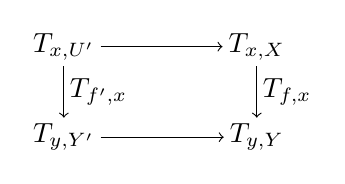
\begin{tikzpicture}[baseline=(current bounding box.center),inner sep=2pt]
  \node (U) at (0,1.15) {$T_{x,U'}$};
  \node (X) at (2.45,1.15) {$T_{x,X}$};
  \node (Yp) at (0,0) {$T_{y,Y'}$};
  \node (Y) at (2.45,0) {$T_{y,Y}$};
  \draw[->] (U) -- (X);
  \draw[->] (U) -- node[right] {$T_{f',x}$} (Yp);
  \draw[->] (X) -- node[right] {$T_{f,x}$} (Y);
  \draw[->] (Yp) -- (Y);
\end{tikzpicture}
\]
The horizontal arrows are injective, because $U'$ and $Y'$ are locally closed subschemes of $X$ and $Y$, respectively. On the other hand, $\operatorname{rank}T_{f,x}\leqslant r$ since $x\in X_r$, and $T_{f',x}$ is surjective because $f'$ is smooth (\Goto{result-III-10.4}{10.4}). We conclude that $\dim T_{y,Y'}\leqslant r$, and therefore $\dim Y'\leqslant r$.

\par\smallskip\noindent\hypertarget{result-III-10.7}{}\textbf{Corollary 10.7} (Generic Smoothness). \emph{Let $f\colon X\to Y$ be a morphism of varieties over an algebraically closed field $k$ of characteristic $0$, and assume that $X$ is nonsingular. Then there is a nonempty open subset $V\subseteq Y$ such that $f\colon f^{-1}V\to V$ is smooth.}

\par\smallskip\noindent\textsc{Proof.}\enspace We may assume $Y$ is nonsingular by (II, \Goto{result-II-8.16}{8.16}). Let $r=\dim Y$. Let $X_{r-1}\subseteq X$ be the subset defined in (\Goto{result-III-10.6}{10.6}). Then $\dim\overline{f(X_{r-1})}\leqslant r-1$ by (\Goto{result-III-10.6}{10.6}), so removing it from $Y$, we may assume that $\operatorname{rank}T_f\geqslant r$ for every closed point of $X$. But since $Y$ is nonsingular of dimension $r$, this implies that $T_f$ is surjective for every closed point of $X$. Hence $f$ is smooth by (\Goto{result-III-10.4}{10.4}).

Note that if the original $f$ was not dominant, then $V\subseteq Y-\overline{f(X)}$, and $f^{-1}V$ will be empty.

\medskip
For the next results, we recall the notion of a group variety (I, Ex.~\Goto{ex-I-3.21}{3.21}). A \emph{group variety} $G$ over an algebraically closed field $k$ is a variety $G$, together
}
% Contents from body/page-287.tex.
% Original printed page 273.
\ChapterSheet[11.45]{287}{273}{\Goto{sec-III-10}{10\quad Smooth Morphisms}}{%
with morphisms $\mu\colon G\times G\to G$ and $\rho\colon G\to G$, such that the set $G(k)$ of $k$-rational points of $G$ (which is just the set of all closed points of $G$, since $k$ is algebraically closed) becomes a group under the operation induced by $\mu$, with $\rho$ giving the inverses.

We say that a group variety $G$ \emph{acts} on a variety $X$ if we have a morphism $\theta\colon G\times X\to X$ which induces a homomorphism $G(k)\to\operatorname{Aut}X$ of groups.

A \emph{homogeneous space} is a variety $X$, together with a group variety $G$ acting on it, such that the group $G(k)$ acts transitively on the set $X(k)$ of $k$-rational points of $X$.

\AuditItem{result-III-10.7.1}{Remark 10.7.1.} Any group variety is a homogeneous space if we let it act on itself by left multiplication.

\AuditItem{result-III-10.7.2}{Example 10.7.2.} The projective space $\mathbf P_k^n$ is a homogeneous space for the action of $G=\operatorname{PGL}(n)$---cf. (II, \Goto{result-II-7.1.1}{7.1.1}).

\AuditItem{result-III-10.7.3}{Example 10.7.3.} A homogeneous space is necessarily a nonsingular variety. Indeed, it has an open subset which is nonsingular by (II, \Goto{result-II-8.16}{8.16}). But we have a transitive group of automorphisms acting, so it is nonsingular everywhere.

\par\smallskip\noindent\hypertarget{result-III-10.8}{}\textbf{Theorem 10.8} (Kleiman \Goto{bib-kleiman-3}{[3]}). \emph{Let $X$ be a homogeneous space with group variety $G$ over an algebraically closed field $k$ of characteristic $0$. Let $f\colon Y\to X$ and $g\colon Z\to X$ be morphisms of nonsingular varieties $Y,Z$ to $X$. For any $\sigma\in G(k)$, let $Y^\sigma$ be $Y$ with the morphism $\sigma\circ f$ to $X$. Then there is a nonempty open subset $V\subseteq G$ such that for every $\sigma\in V(k)$, $Y^\sigma\times_X Z$ is nonsingular and either empty or of dimension exactly}
\[
 \dim Y+\dim Z-\dim X.
\]

\noindent\textsc{Proof.}\enspace First we consider the morphism
\[
 h\colon G\times Y\to X
\]
defined by composing $f$ with the group action $\theta\colon G\times X\to X$. Now $G$ is nonsingular since it is a group variety (\Goto{result-III-10.7.3}{10.7.3}), and $Y$ is nonsingular by hypothesis, so $G\times Y$ is nonsingular by (\Goto{result-III-10.1}{10.1}). Since $\operatorname{char}k=0$, we can apply generic smoothness (\Goto{result-III-10.7}{10.7}) to $h$, and conclude that there is a nonempty open subset $U\subseteq X$ such that $h\colon h^{-1}(U)\to U$ is smooth. Now $G$ acts on $G\times Y$ by left multiplication on $G$; $G$ acts on $X$ by $\theta$, and these two actions are compatible with the morphism $h$, by construction. Therefore, for any $\sigma\in G(k)$, $h\colon h^{-1}(U^\sigma)\to U^\sigma$ is also smooth. Since the $U^\sigma$ cover $X$, we conclude that $h$ is smooth everywhere.

Next, we consider the fibred product
\[
 W=(G\times Y)\times_X Z,
\]
with maps $g'$ and $h'$ to $G\times Y$ and $Z$ as shown.
}
% Contents from body/page-288.tex.
% Original printed page 274.
\ChapterSheet[11.35]{288}{274}{\Goto{p-215}{III\quad Cohomology}}{%
\noindent\makebox[\linewidth][c]{%
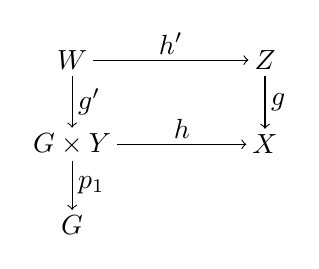
\begin{tikzpicture}[baseline=(current bounding box.center),inner sep=2pt]
  \node (W) at (0,2.1) {$W$};
  \node (Z) at (2.45,2.1) {$Z$};
  \node (GY) at (0,1.03) {$G\times Y$};
  \node (X) at (2.45,1.03) {$X$};
  \node (G) at (0,0) {$G$};
  \draw[->] (W) -- node[above] {$h'$} (Z);
  \draw[->] (GY) -- node[above] {$h$} (X);
  \draw[->] (W) -- node[right] {$g'$} (GY);
  \draw[->] (Z) -- node[right] {$g$} (X);
  \draw[->] (GY) -- node[right] {$p_1$} (G);
\end{tikzpicture}}\par\medskip\noindent
Since $h$ is smooth, $h'$ is also smooth by base extension (\Goto{result-III-10.1}{10.1}). Since $Z$ is nonsingular, it is smooth over $k$, so by composition (\Goto{result-III-10.1}{10.1}), $W$ is also smooth over $k$, so $W$ is nonsingular.

Now we consider the morphism
\[
 q=p_1\circ g'\colon W\to G.
\]
Applying generic smoothness (\Goto{result-III-10.7}{10.7}) again, we find there is a nonempty open subset $V\subseteq G$ such that $q\colon q^{-1}(V)\to V$ is smooth. Therefore, if $\sigma\in V(k)$ is any closed point, the fibre $W_\sigma$ will be nonsingular. But $W_\sigma$ is just $Y^\sigma\times_X Z$, so this is what we wanted to show. Note that $W_\sigma$ may not be irreducible, but our result shows that each connected component is a nonsingular variety.

To find the dimension of $W_\sigma$, we first note that $h$ is smooth of relative dimension
\[
 \dim G+\dim Y-\dim X.
\]
Hence $h'$ has the same relative dimension, and we see that \EditionText{if $W$ is nonempty, all its components have dimension}
\[
 \EditionText{}
 \dim G+\dim Y-\dim X+\dim Z.
\]
\EditionText{For each nonempty fibre $W_\sigma$ over $V$, smoothness gives dimension $\dim W-\dim G$, so}
\[
 \dim W_\sigma=\dim Y+\dim Z-\dim X.
\]

\par\smallskip\noindent\hypertarget{result-III-10.9}{}\textbf{Corollary 10.9} (Bertini). \emph{Let $X$ be a nonsingular projective variety over an algebraically closed field $k$ of characteristic $0$. Let $\mathfrak d$ be a linear system without base points. Then almost every element of $\mathfrak d$, considered as a closed subscheme of $X$, is nonsingular (but maybe reducible).}

\par\smallskip\noindent\textsc{Proof.}\enspace Let $f\colon X\to\mathbf P^n$ be the morphism to $\mathbf P^n$ determined by $\mathfrak d$ (II, \Goto{result-II-7.8.1}{7.8.1}). \EditionText{If $n=0$, the single member of the base-point-free system is the empty divisor. Suppose $n\geqslant1$. }We consider $\mathbf P^n$ as a homogeneous space under the action of $G=\operatorname{PGL}(n)$ (\Goto{result-III-10.7.2}{10.7.2}). We apply the theorem taking $g\colon H\to\mathbf P^n$ to be the inclusion map of a hyperplane $H\cong\mathbf P^{n-1}$. We conclude that for almost all $\sigma\in G(k)$, $X\times_{\mathbf P^n}H^\sigma=f^{-1}(H^\sigma)$ is nonsingular. But the divisors $f^{-1}(H^\sigma)$ are just the elements of the linear system $\mathfrak d$, by construction of $f$. Thus almost all elements of $\mathfrak d$ are nonsingular.
}
% Contents from body/page-289.tex.
% Original printed page 275.
\ChapterSheet[11.1]{289}{275}{\Goto{sec-III-10}{10\quad Smooth Morphisms}}{%
\AuditItem{result-III-10.9.1}{Remark 10.9.1.} We will see later (Ex.~\Goto{ex-III-11.3}{11.3}) that if $\dim f(X)\geqslant2$, then all the divisors in $\mathfrak d$ are connected. Hence almost all of them are irreducible and nonsingular.

\AuditItem{result-III-10.9.2}{Remark 10.9.2.} The hypothesis \textquotedblleft $X$ projective\textquotedblright\ is not necessary if we talk about a finite-dimensional linear system $\mathfrak d$. In particular, if $X$ was projective, and $\mathfrak d$ was a linear system with base points $\Sigma$, then by considering the base-point-free linear system $\mathfrak d$ on $X-\Sigma$ we obtain the more general statement that \textquotedblleft a general member of $\mathfrak d$ can have singularities only at the base points.\textquotedblright

\AuditItem{result-III-10.9.3}{Remark 10.9.3.} This result fails in characteristic $p>0$. For example, in (\Goto{result-III-10.5.1}{10.5.1}) the morphism $f$ corresponds to the one-dimensional linear system $\{pP\mid P\in\mathbf P^1\}$. Thus every divisor in $\mathfrak d$ is a point with multiplicity $p$.

\AuditItem{result-III-10.9.4}{Remark 10.9.4.} Compare this result to the earlier Bertini theorem (II, \Goto{result-II-8.18}{8.18}).

\par\medskip\noindent\textsc{Exercises}\par
\AuditItem{ex-III-10.1}{10.1.} Over a nonperfect field, smooth and regular are not equivalent. For example, let $k_0$ be a field of characteristic $p>0$, let $k=k_0(t)$, and let $X\subseteq\mathbf A_k^2$ be the curve defined by $y^2=x^p-t$. Show that every local ring of $X$ is a regular local ring, but $X$ is not smooth over $k$.

\AuditItem{ex-III-10.2}{10.2.} Let $f\colon X\to Y$ be a proper, flat morphism of varieties over $k$. Suppose for some point $y\in Y$ that the fibre $X_y$ is smooth over $k(y)$. Then show that there is an open neighborhood $U$ of $y$ in $Y$ such that $f\colon f^{-1}(U)\to U$ is smooth.

\AuditItem{ex-III-10.3}{10.3.} A morphism $f\colon X\to Y$ of schemes of finite type over $k$ is \emph{\'etale} if it is smooth of relative dimension $0$. It is \emph{unramified} if for every $x\in X$, letting $y=f(x)$, we have $\mathfrak m_y\cdot\mathcal O_x=\mathfrak m_x$, and $k(x)$ is a separable algebraic extension of $k(y)$. Show that the following conditions are equivalent:
\begin{enumerate}[label=(\roman*),leftmargin=2.7em,itemsep=0pt,topsep=1pt,parsep=0pt]
\item $f$ is \'etale;
\item $f$ is flat, and $\Omega_{X/Y}=0$;
\item $f$ is flat and unramified.
\end{enumerate}

\AuditItem{ex-III-10.4}{10.4.} Show that a morphism $f\colon X\to Y$ of schemes of finite type over $k$ is \'etale if and only if the following condition is satisfied: for each $x\in X$, let $y=f(x)$. Let $\widehat{\mathcal O}_x$ and $\widehat{\mathcal O}_y$ be the completions of the local rings at $x$ and $y$. \EditionText{First require $k(x)/k(y)$ to be finite and separable. Choose a field of representatives $k(y)\subseteq\widehat{\mathcal O}_y$ (II, \Goto{result-II-8.25A}{8.25A}), and lift $k(x)$ to a field of representatives in $\widehat{\mathcal O}_x$ compatible with the map $\widehat{\mathcal O}_y\to\widehat{\mathcal O}_x$. Then require that the natural map}
\[
 \widehat{\mathcal O}_y\otimes_{k(y)}k(x)\to\widehat{\mathcal O}_x
\]
is an isomorphism.

\AuditItem{ex-III-10.5}{10.5.} If $x$ is a point of a scheme $X$, we define an \emph{\'etale neighborhood} of $x$ to be an \'etale morphism $f\colon U\to X$, together with a point $x'\in U$ such that $f(x')=x$. As an example of the use of \'etale neighborhoods, prove the following: if $\mathcal F$ is a coherent sheaf on $X$, and if every point of $X$ has an \'etale neighborhood $f\colon U\to X$ for which $f^*\mathcal F$ is a free $\mathcal O_U$-module, then $\mathcal F$ is locally free on $X$.
}
% Contents from body/page-290.tex.
% Original printed page 276.
\BookMark{1}{3.11  The Theorem on Formal Functions}{sec-III-11}
\ChapterSheet[10.75]{290}{276}{\Goto{p-215}{III\quad Cohomology}}{%
\AuditItem{ex-III-10.6}{10.6.} \EditionText{Assume $\operatorname{char}k\ne2$. }Let $Y$ be the plane nodal cubic curve $y^2=x^2(x+1)$. Show that $Y$ has a finite \'etale covering $X$ of degree $2$, where $X$ is a union of two irreducible components, each one isomorphic to the normalization of $Y$ (Fig.~\Goto{fig-book-12}{12}).

\par\smallskip\noindent\resizebox{\linewidth}{!}{% Figure 12. A finite etale covering (printed page 276).
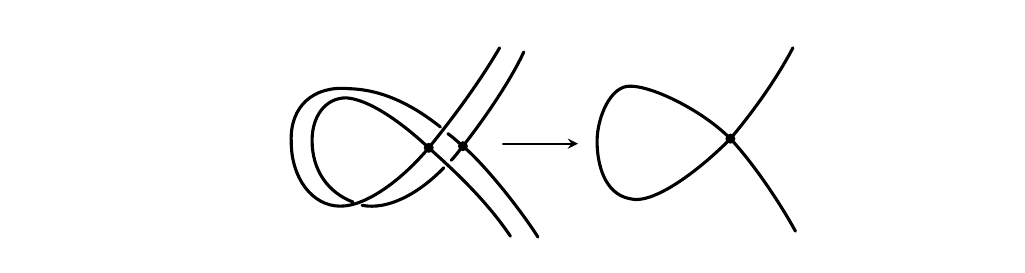
\begin{tikzpicture}[
    x=.3bp, y=-.3bp, line cap=round, line join=round, >=stealth,
    branch/.style={line width=1.12bp}
  ]
  \path[use as bounding box] (-298.3,-10.2) rectangle (865.033,250.133);
  \coordinate (first-node) at (183,134);
  \coordinate (second-node) at (224,132);

  % One component passes behind the other near its upper arc.
  \draw[branch] (268,14)
    .. controls (244,55) and (213,97) .. (first-node)
    .. controls (152,171) and (109,204) .. (77,204)
    .. controls (43,204) and (18,170) .. (18,127)
    .. controls (16,84) and (45,59) .. (87,63)
    .. controls (127,64) and (163,82) .. (197,109);
  \draw[branch] (206,117)
    .. controls (213,122) and (218,127) .. (second-node)
    .. controls (249,153) and (291,205) .. (314,241);

  % The other underpasses lie just below the two crossings.
  \draw[branch] (297,19)
    .. controls (282,52) and (250,99) .. (second-node)
    .. controls (219,138) and (214,145) .. (210,149);
  \draw[branch] (201,158)
    .. controls (171,189) and (134,209) .. (103,203);
  \draw[branch] (92,199)
    .. controls (63,188) and (43,162) .. (43,125)
    .. controls (43,96) and (59,74) .. (84,74)
    .. controls (112,76) and (151,104) .. (first-node)
    .. controls (219,166) and (254,200) .. (281,240);
  \fill (first-node) circle[radius=1.8bp];
  \fill (second-node) circle[radius=1.8bp];

  \draw[->,line width=.61bp] (272,129) -- (362,129);

  \coordinate (node) at (545,123);
  \draw[branch] (620,14)
    .. controls (600,52) and (572,91) .. (node)
    .. controls (517,152) and (455,204) .. (424,195)
    .. controls (394,189) and (385,154) .. (385,126)
    .. controls (385,98) and (401,59) .. (425,60)
    .. controls (451,60) and (510,88) .. (node)
    .. controls (572,152) and (604,199) .. (623,234);
  \fill (node) circle[radius=1.8bp];
\end{tikzpicture}
}\par
\noindent\makebox[\linewidth][c]{\small\hypertarget{fig-book-12}{}\textbf{Figure 12.}\enspace A finite \'etale covering.}\par

\AuditItem{ex-III-10.7}{10.7.} (Serre). \emph{A linear system with moving singularities.} Let $k$ be an algebraically closed field of characteristic $2$. Let $P_1,\ldots,P_7\in\mathbf P^2_k$ be the seven points of the projective plane over the prime field $\mathbf F_2\subseteq k$.\EditionText{ Put $X=\mathbf P^2_k$.} Let $\mathfrak d$ be the linear system of all cubic curves in $X$ passing through $P_1,\ldots,P_7$.
\begin{enumerate}[label=(\alph*),leftmargin=2.7em,itemsep=0pt,topsep=1pt,parsep=0pt]
\item $\mathfrak d$ is a linear system of dimension $2$ with base points $P_1,\ldots,P_7$, which determines an inseparable morphism of degree $2$ from $X-\{P_i\}$ to $\mathbf P^2$.
\item Every curve $C\in\mathfrak d$ is singular. More precisely, either $C$ consists of $3$ lines all passing through one of the $P_i$, or $C$ is an irreducible cuspidal cubic with cusp $P\ne$ any $P_i$. Furthermore, the correspondence $C\mapsto$ the singular point of $C$ is a 1-1 correspondence between $\mathfrak d$ and $\mathbf P^2$. Thus the singular points of elements of $\mathfrak d$ move all over.
\end{enumerate}

\AuditItem{ex-III-10.8}{10.8.} \emph{A linear system with moving singularities contained in the base locus (any characteristic).} \EditionText{Use projective coordinates $(X:Y:Z:W)$ on $\mathbf P^3$. In the plane $Z=0$ let $C$ be the conic $X^2-YW=0$. For $t\ne0$, take the cone $Y_t$ over $C$ with vertex $P=(0:0:t:1)$, and complete these cones to the pencil spanned by $X^2-YW$ and $YZ$. Show that this is a linear system of dimension $1$, with a moving singularity at $P$ for $t\ne0$. Show that the underlying set of the base locus is the conic $C$ together with the $z$-axis.}

\AuditItem{ex-III-10.9}{10.9.} Let $f\colon X\to Y$ be a morphism of varieties over $k$. Assume that $Y$ is regular, $X$ is Cohen--Macaulay, and that every fibre of $f$ has dimension equal to $\dim X-\dim Y$. Then $f$ is flat. [\emph{Hint:} Imitate the proof of (\Goto{result-III-10.4}{10.4}), using (II, \Goto{result-II-8.21A}{8.21A}).]

\par\medskip\noindent\hypertarget{sec-III-11}{}{\large\bfseries 11\enspace The Theorem on Formal Functions}\par\medskip
\noindent In this section we prove the so-called theorem on formal functions, and its important corollaries, Zariski's Main Theorem, and the Stein factorization theorem. The theorem itself compares the cohomology of the infinitesimal neighborhoods of a fibre of a projective morphism to the stalk of the higher direct image sheaves. While the corollaries use only the case $i=0$ of the theorem (which could be stated without cohomology), the proof is by descending induction on $i$, and thus makes essential use of the cohomological machinery. Zariski's first proof \Goto{bib-zariski-2}{[2]} of his \textquotedblleft Main Theorem\textquotedblright\ was by an entirely different method which did not use cohomology.

Let $f\colon X\to Y$ be a projective morphism of noetherian schemes, let $\mathcal F$ be a coherent sheaf on $X$, and let $y\in Y$ be a point. For each $n\geqslant1$ we
}
% Contents from body/page-291.tex.
% Original printed page 277.
\ChapterSheet[11.1]{291}{277}{\Goto{sec-III-11}{11\quad The Theorem on Formal Functions}}{%
define
\[
 X_n=X\times_Y\operatorname{Spec}\mathcal O_y/\mathfrak m_y^n.
\]
Then for $n=1$, we get the fibre $X_y$, and for $n>1$, we get a \EditionText{possibly nonreduced scheme with the same underlying space as $X_y$.} It is a kind of \textquotedblleft thickened fibre\textquotedblright\ of $X$ over the point $y$.
\[
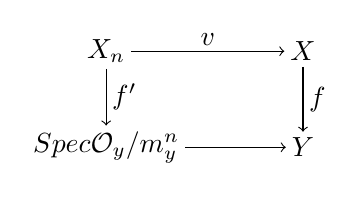
\begin{tikzpicture}[baseline=(current bounding box.center),inner sep=2pt]
  \node (a) at (0,1.22) {$X_n$};
  \node (b) at (2.5,1.22) {$X$};
  \node (c) at (0,0) {$\operatorname{Spec}\mathcal O_y/\mathfrak m_y^n$};
  \node (d) at (2.5,0) {$Y$};
  \draw[->] (a) -- node[above] {$v$} (b);
  \draw[->] (a) -- node[right] {$f'$} (c);
  \draw[->] (b) -- node[right] {$f$} (d);
  \draw[->] (c) -- (d);
\end{tikzpicture}
\]
Let $\mathcal F_n=v^*\mathcal F$, where $v\colon X_n\to X$ is the natural map. Then by (\Goto{result-III-9.3.1}{9.3.1}) we have natural maps, for each $n$,
\[
 R^if_*(\mathcal F)\otimes\mathcal O_y/\mathfrak m_y^n\to R^if'_*(\mathcal F_n).
\]
Since $\operatorname{Spec}\mathcal O_y/\mathfrak m_y^n$ is affine, concentrated at one point, the right-hand side is just the group $H^i(X_n,\mathcal F_n)$ by (\Goto{result-III-8.5}{8.5}). As $n$ varies, both sides form inverse systems (see (II, \S\Goto{sec-II-9}{9}) for generalities on inverse systems and inverse limits). Thus we can take inverse limits and get a natural map
\[
 R^if_*(\mathcal F)_y^{\wedge}\to\varprojlim H^i(X_n,\mathcal F_n).
\]

\par\smallskip\noindent\hypertarget{result-III-11.1}{}\textbf{Theorem 11.1} (Theorem on Formal Functions). \emph{Let $f\colon X\to Y$ be a projective morphism of noetherian schemes, let $\mathcal F$ be a coherent sheaf on $X$, and let $y\in Y$. Then the natural map}
\[
 R^if_*(\mathcal F)_y^{\wedge}\to\varprojlim H^i(X_n,\mathcal F_n)
\]
\noindent\emph{is an isomorphism, for all $i\geqslant0$.}

\par\smallskip\noindent\textsc{Proof.}\enspace As a first step, we embed $X$ in some projective space $\mathbf P_Y^N$, and consider $\mathcal F$ as a coherent sheaf on $\mathbf P_Y^N$. Thus we reduce to the case $X=\mathbf P_Y^N$.

Next we let $A=\mathcal O_y$, and make the flat base extension $\operatorname{Spec}A\to Y$. Thus, using (\Goto{result-III-9.3}{9.3}), we reduce to the case where $Y$ is affine, equal to the spectrum of a local noetherian ring $A$, and $y$ is the closed point of $Y$. Then using (\Goto{result-III-8.5}{8.5}) again, we can restate our result as an isomorphism of $A$-modules,
\[
 H^i(X,\mathcal F)^\wedge\cong\varprojlim H^i(X_n,\mathcal F_n).
\]
Now suppose $\mathcal F$ is a sheaf of the form $\mathcal O(q)$ on $X=\mathbf P_A^N$, for some $q\in\mathbf Z$. Then $\mathcal F_n$ is just $\mathcal O(q)$ on $X_n=\mathbf P^N_{A/\mathfrak m^n}$. So by the explicit calculations of (\Goto{result-III-5.1}{5.1}) we see that
\[
 H^i(X_n,\mathcal F_n)\cong H^i(X,\mathcal F)\otimes_A A/\mathfrak m^n
\]
for each $n$. Therefore by definition of completion, we have
\[
 H^i(X,\mathcal F)^\wedge\cong\varprojlim H^i(X_n,\mathcal F_n)
\]
in this case. Clearly the same calculation holds for any finite direct sum of sheaves of the form $\mathcal O(q_i)$.
}
% Contents from body/page-292.tex.
% Original printed page 278.
\ChapterSheet[11.05]{292}{278}{\Goto{p-215}{III\quad Cohomology}}{%
\indent We will now prove the theorem for an arbitrary coherent sheaf $\mathcal F$ on $X$, by descending induction on $i$. For $i>N$, both sides are $0$, because $X$ can be covered by $N+1$ open affine subsets (Ex.~\Goto{ex-III-4.8}{4.8}). So we assume the theorem has been proved for $i+1$, and for all coherent sheaves.

Given $\mathcal F$ coherent on $X$, it follows from (II, \Goto{result-II-5.18}{5.18}) that we can write $\mathcal F$ as a quotient of a sheaf $\mathcal E$ which is a finite direct sum of sheaves $\mathcal O(q_i)$ for suitable $q_i\in\mathbf Z$. Let $\mathcal R$ be the kernel:
\[
 0\to\mathcal R\to\mathcal E\to\mathcal F\to0.\tag{\hypertarget{eq-292-0-1}{}1}
\]
Now unfortunately, tensoring with $\mathcal O_{X_n}$ is not an exact functor---it is only right exact, so we have an exact sequence
\[
 \mathcal R_n\to\mathcal E_n\to\mathcal F_n\to0
\]
of sheaves on $X_n$ for each $n$. We introduce the image $\mathcal T_n$ and the kernel $\mathcal S_n$ of the map $\mathcal R_n\to\mathcal E_n$, so that we have exact sequences
\[
 0\to\mathcal S_n\to\mathcal R_n\to\mathcal T_n\to0\tag{\hypertarget{eq-292-0-2}{}2}
\]
and
\[
 0\to\mathcal T_n\to\mathcal E_n\to\mathcal F_n\to0.\tag{\hypertarget{eq-292-0-3}{}3}
\]
We now consider the following diagram:
\par\smallskip\noindent\makebox[\linewidth][c]{%
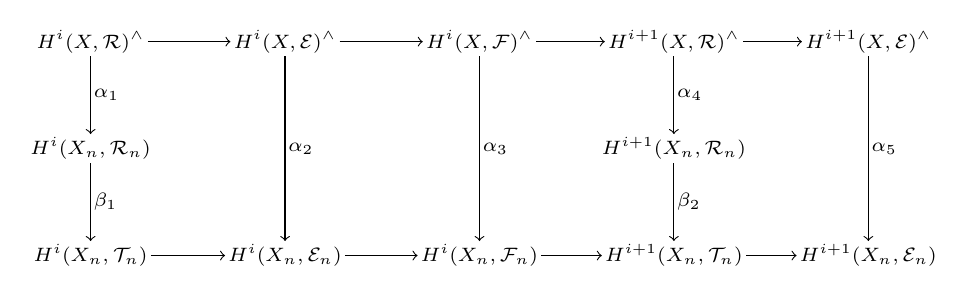
\begin{tikzpicture}[x=1bp,y=1bp,every node/.style={inner sep=1pt,font=\scriptsize}]
  \node (a1) at (0,77) {$H^i(X,\mathcal R)^\wedge$};
  \node (a2) at (70,77) {$H^i(X,\mathcal E)^\wedge$};
  \node (a3) at (140,77) {$H^i(X,\mathcal F)^\wedge$};
  \node (a4) at (210,77) {$H^{i+1}(X,\mathcal R)^\wedge$};
  \node (a5) at (280,77) {$H^{i+1}(X,\mathcal E)^\wedge$};
  \node (b1) at (0,38.5) {$\varprojlim H^i(X_n,\mathcal R_n)$};
  \node (b4) at (210,38.5) {$\varprojlim H^{i+1}(X_n,\mathcal R_n)$};
  \node (c1) at (0,0) {$\varprojlim H^i(X_n,\mathcal T_n)$};
  \node (c2) at (70,0) {$\varprojlim H^i(X_n,\mathcal E_n)$};
  \node (c3) at (140,0) {$\varprojlim H^i(X_n,\mathcal F_n)$};
  \node (c4) at (210,0) {$\varprojlim H^{i+1}(X_n,\mathcal T_n)$};
  \node (c5) at (280,0) {$\varprojlim H^{i+1}(X_n,\mathcal E_n)$};
  \foreach \n/\next in {1/2,2/3,3/4,4/5}{
    \draw[->] (a\n) -- (a\next);
    \draw[->] (c\n) -- (c\next);
  }
  \draw[->] (a1) -- node[right] {$\alpha_1$} (b1);
  \draw[->] (a2) -- node[right] {$\alpha_2$} (c2);
  \draw[->] (a3) -- node[right] {$\alpha_3$} (c3);
  \draw[->] (a4) -- node[right] {$\alpha_4$} (b4);
  \draw[->] (a5) -- node[right] {$\alpha_5$} (c5);
  \draw[->] (b1) -- node[right] {$\beta_1$} (c1);
  \draw[->] (b4) -- node[right] {$\beta_2$} (c4);
\end{tikzpicture}}\par\smallskip\noindent
The top row comes from the cohomology sequence of (\Goto{eq-292-0-1}{1}) by completion. Since they are all finitely generated $A$-modules (\Goto{result-III-5.2}{5.2}), completion is an exact functor (II, \Goto{result-II-9.3A}{9.3A}). The bottom row comes from the cohomology sequence of (\Goto{eq-292-0-3}{3}) by taking inverse limits. These groups are all finitely generated $A/\mathfrak m^n$-modules, and so satisfy d.c.c.\ for submodules. Therefore the inverse systems all satisfy the Mittag--Leffler condition (II, \Goto{result-II-9.1.2}{9.1.2}), and so the bottom row is exact (II, \Goto{result-II-9.1}{9.1}). The vertical arrows $\alpha_1,\ldots,\alpha_5$ are the maps of the theorem. We have $\alpha_2$ an isomorphism because $\mathcal E$ is a sum of sheaves $\mathcal O(q_i)$, and $\alpha_4$ and $\alpha_5$ are isomorphisms by the induction hypothesis. Finally, $\beta_1$ and $\beta_2$ are maps induced from the sequence (\Goto{eq-292-0-2}{2}). We will show below that $\beta_1$ and $\beta_2$ are isomorphisms.

Admitting this for the moment, it follows from the subtle 5-lemma that $\alpha_3$ is surjective. But this is then true for any coherent sheaf on $X$, so $\alpha_1$ must also be surjective. This in turn implies $\alpha_3$ is an isomorphism, which is what we want.
}
% Contents from body/page-293.tex.
% Original printed page 279.
\ChapterSheet[11.35]{293}{279}{\Goto{sec-III-11}{11\quad The Theorem on Formal Functions}}{%
\indent It remains to prove that $\beta_1$ and $\beta_2$ are isomorphisms. Taking the cohomology sequence of (\Goto{eq-292-0-2}{2}), and passing to the inverse limit, using (II, \Goto{result-II-9.1}{9.1}) again, it will be sufficient to show that
\[
 \varprojlim H^i(X_n,\mathcal S_n)=0
\]
for all $i\geqslant0$. To accomplish this, we will show that for any $n$, there is an $n'>n$ such that the map of sheaves $\mathcal S_{n'}\to\mathcal S_n$ is the zero map. By quasi-compactness, the question is local on $X$, so we may assume that $X$ is affine, $X=\operatorname{Spec}B$. We denote by $R,E,S_n$ the $B$-modules corresponding to the sheaves $\mathcal R,\mathcal E,\mathcal S_n$, and we denote by $\mathfrak a$ the ideal $\mathfrak mB$.

Recall that $R$ is a submodule of $E$, and that
\[
 S_n=\ker(R/\mathfrak a^nR\to E/\mathfrak a^n E).
\]
Thus
\[
 S_n=(R\cap\mathfrak a^n E)/\mathfrak a^nR.
\]
But by Krull's theorem (\Goto{result-III-3.1A}{3.1A}), the $\mathfrak a$-adic topology on $R$ is induced by the $\mathfrak a$-adic topology on $E$. In other words, for any $n$, there is an $n'>n$ such that
\[
 R\cap\mathfrak a^{n'}E\subseteq\mathfrak a^nR.
\]
In that case the map $S_{n'}\to S_n$ is zero.\nobreak\hfill q.e.d.

\AuditItem{result-III-11.1.1}{Remark 11.1.1.} This theorem is proved more generally for a proper morphism in Grothendieck \Goto{bib-ega-iii}{[EGA III, \S4]}.

\AuditItem{result-III-11.1.2}{Remark 11.1.2.} Many applications of this theorem use only the case $i=0$. In that case the right-hand side is equal to $\Gamma(\widehat X,\widehat{\mathcal F})$, \EditionText{where $\widehat X$ is the formal completion of $X_{\mathrm{loc}}=X\times_Y\operatorname{Spec}\mathcal O_{Y,y}$ along its closed fibre $X_y$, and $\widehat{\mathcal F}$ is the completion of the pullback of $\mathcal F$ to $X_{\mathrm{loc}}$} (II, \Goto{result-II-9.2}{9.2}). In particular, if $\mathcal F=\mathcal O_X$, we have $\Gamma(\widehat X,\mathcal O_{\widehat X})$, which is the ring of \emph{formal-regular functions} (also called \emph{holomorphic functions}) on \EditionText{$X_{\mathrm{loc}}$} along $X_y$. Hence the name of the theorem.

\AuditItem{result-III-11.1.3}{Remark 11.1.3.} One can also introduce the cohomology $H^i(\widehat X,\widehat{\mathcal F})$ of $\widehat{\mathcal F}$ on the formal scheme $\widehat X$, and prove that it is isomorphic to the two other quantities in the theorem \Goto{bib-ega-iii}{[EGA III, \S4]}.

\AuditItem{result-III-11.2}{Corollary 11.2.} \emph{Let $f\colon X\to Y$ be a projective morphism of noetherian schemes, and let $r=\max\{\dim X_y\mid y\in Y\}$. Then $R^if_*(\mathcal F)=0$ for all $i>r$, and for all coherent sheaves $\mathcal F$ on $X$.}

\par\smallskip\noindent\textsc{Proof.}\enspace For any $y\in Y$, $X_n$ is a scheme whose underlying topological space is the same as $X_y$. Hence
\[
 H^i(X_n,\mathcal F_n)=0
\]
for $i>r$ by (\Goto{result-III-2.7}{2.7}). It follows that $R^if_*(\mathcal F)_y^\wedge=0$ for all $y\in Y$, $i>r$, and therefore since $R^if_*(\mathcal F)$ is coherent (\Goto{result-III-8.8}{8.8}) it must be $0$.

\AuditItem{result-III-11.3}{Corollary 11.3.} \emph{Let $f\colon X\to Y$ be a projective morphism of noetherian schemes, and assume that $f_*\mathcal O_X=\mathcal O_Y$. Then $f^{-1}(y)$ is connected, for every $y\in Y$.}
}
% Contents from body/page-294.tex.
% Original printed page 280.
\ChapterSheet[10.95]{294}{280}{\Goto{p-215}{III\quad Cohomology}}{%
\textsc{Proof.}\enspace Suppose to the contrary that $f^{-1}(y)=X'\cup X''$, where $X'$ and $X''$ are disjoint closed subsets. Then for each $n$, we would have
\[
 H^0(X_n,\mathcal O_{X_n})=H^0(X'_n,\mathcal O_{X_n})\oplus H^0(X''_n,\mathcal O_{X_n}).
\]
By the theorem, we have
\[
 \widehat{\mathcal O}_y=(f_*\mathcal O_X)^\wedge_y
   =\varprojlim H^0(X_n,\mathcal O_{X_n}).
\]
Therefore $\widehat{\mathcal O}_y=A'\oplus A''$, where
\[
 A'=\varprojlim H^0(X'_n,\mathcal O_{X_n})
\]
and
\[
 A''=\varprojlim H^0(X''_n,\mathcal O_{X_n}).
\]
But this is impossible, because a local ring cannot be a direct sum of two other rings. Indeed, let $e',e''$ be the unit elements of $A'$ and $A''$. Then $e'+e''=1$ in $\widehat{\mathcal O}_y$. On the other hand, $e'e''=0$, so $e',e''$ are nonunits, hence contained in the maximal ideal of $\widehat{\mathcal O}_y$, so their sum cannot be $1$ (cf. (II, Ex.~\Goto{ex-II-2.19}{2.19})).

\par\smallskip\noindent\hypertarget{result-III-11.4}{}\textbf{Corollary 11.4} (Zariski's Main Theorem). \emph{Let $f\colon X\to Y$ be a birational projective morphism of noetherian integral schemes, and assume that $Y$ is normal. Then for every $y\in Y$, $f^{-1}(y)$ is connected.} (See also (V, \Goto{result-V-5.2}{5.2}).)

\par\smallskip\noindent\textsc{Proof.}\enspace By the previous result, we have only to verify that $f_*\mathcal O_X=\mathcal O_Y$. The question is local on $Y$, so we may assume $Y$ is affine, equal to $\operatorname{Spec}A$. Then $f_*\mathcal O_X$ is a coherent sheaf of $\mathcal O_Y$-algebras, so $B=\Gamma(Y,f_*\mathcal O_X)$ is a finitely generated $A$-module. But $A$ and $B$ are integral domains with the same quotient field, and $A$ is integrally closed, so we must have $A=B$. Thus $f_*\mathcal O_X=\mathcal O_Y$.

\par\smallskip\noindent\hypertarget{result-III-11.5}{}\textbf{Corollary 11.5} (Stein Factorization). \emph{Let $f\colon X\to Y$ be a projective morphism of noetherian schemes. Then one can factor $f$ into $g\circ f'$, where $f'\colon X\to Y'$ is a projective morphism with connected fibres, and $g\colon Y'\to Y$ is a finite morphism.}

\par\smallskip\noindent\textsc{Proof.}\enspace Let $Y'=\mathbf{Spec}f_*\mathcal O_X$ (II, Ex.~\Goto{ex-II-5.17}{5.17}). Then since $f_*\mathcal O_X$ is a coherent sheaf of $\mathcal O_Y$-algebras, the natural map $g\colon Y'\to Y$ is finite. On the other hand $f$ clearly factors through $g$, so we get a morphism $f'\colon X\to Y'$. Since $g$ is separated, we conclude that $f'$ is projective by (II, Ex.~\Goto{ex-II-4.9}{4.9}). By construction $f'_*\mathcal O_X=\mathcal O_{Y'}$ so $f'$ has connected fibres by (\Goto{result-III-11.3}{11.3}).

\par\smallskip\noindent\textsc{Exercises}\par
\AuditItem{ex-III-11.1}{11.1.} Show that the result of (\Goto{result-III-11.2}{11.2}) is false without the projective hypothesis. For example, let $X=\mathbf A_k^n$\EditionText{ with $n\geqslant2$}, let $P=(0,\ldots,0)$, let $U=X-P$, and let $f\colon U\to X$ be the inclusion. Then the \EditionText{nonempty fibres of $f$ have} dimension $0$, but $R^{n-1}f_*\mathcal O_U\ne0$.

\AuditItem{ex-III-11.2}{11.2.} Show that a projective morphism with finite fibres ($=$ quasi-finite (II, Ex.~\Goto{ex-II-3.5}{3.5})) is a finite morphism.

\AuditItem{ex-III-11.3}{11.3.} Let $X$ be a normal, projective variety over an algebraically closed field $k$. Let $\mathfrak d$ be a linear system (of effective Cartier divisors) without base points, and assume that $\mathfrak d$ is \emph{not composite with a pencil}, which means that if $f\colon X\to\mathbf P_k^n$ is the morphism
}
% Contents from body/page-295.tex.
% Original printed page 281.
\BookMark{1}{3.12  The Semicontinuity Theorem}{sec-III-12}
\ChapterSheet[10.4]{295}{281}{\Goto{sec-III-12}{12\quad The Semicontinuity Theorem}}{%
\setlength{\parskip}{0pt}%
determined by $\mathfrak d$, then $\dim f(X)\geqslant2$. Then show that every divisor in $\mathfrak d$ is connected. This improves Bertini's theorem (\Goto{result-III-10.9.1}{10.9.1}). [\emph{Hints:} Use (\Goto{result-III-11.5}{11.5}), (Ex.~\Goto{ex-III-5.7}{5.7}) and (\Goto{result-III-7.9}{7.9}).]

\AuditItem{ex-III-11.4}{11.4.} \emph{Principle of Connectedness.} Let $\{X_t\}$ be a flat family of closed subschemes of $\mathbf P_k^n$ parametrized by an irreducible curve $T$ of finite type over $k$. Suppose there is a nonempty open set $U\subseteq T$, such that for all closed points $t\in U$, $X_t$ is connected. Then prove that $X_t$ is connected for all $t\in T$.

\AuditItem{ex-III-11.5}{*11.5.} Let $Y$ be a hypersurface in $X=\mathbf P_k^N$ with $N\geqslant4$. Let $\widehat X$ be the formal completion of $X$ along $Y$ (II, \S\Goto{sec-II-9}{9}). Prove that the natural map $\operatorname{Pic}\widehat X\to\operatorname{Pic}Y$ is an isomorphism. [\emph{Hint:} Use (II, Ex.~\Goto{ex-II-9.6}{9.6}), and then study the maps $\operatorname{Pic}X_{n+1}\to\operatorname{Pic}X_n$ for each $n$ using (Ex.~\Goto{ex-III-4.6}{4.6}) and (Ex.~\Goto{ex-III-5.5}{5.5}).]

\AuditItem{ex-III-11.6}{11.6.} Again let $Y$ be a hypersurface in $X=\mathbf P_k^N$, this time with $N\geqslant2$.
\begin{enumerate}[label=(\alph*),leftmargin=2.7em,itemsep=0pt,topsep=1pt,parsep=0pt]
\item\hypertarget{ex-III-11.6a}{} If $\mathcal F$ is a locally free sheaf on $X$, show that the natural map
\[
 H^0(X,\mathcal F)\to H^0(\widehat X,\widehat{\mathcal F})
\]
is an isomorphism.
\item\hypertarget{ex-III-11.6b}{} Show that the following conditions are equivalent:
\begin{enumerate}[label=(\roman*),leftmargin=2.4em,itemsep=0pt,topsep=1pt,parsep=0pt]
\item\hypertarget{ex-III-11.6bi}{} for each locally free sheaf $\mathfrak F$ on $\widehat X$, there exists a coherent sheaf $\mathcal F$ on $X$ such that $\mathfrak F\cong\widehat{\mathcal F}$ (i.e., $\mathfrak F$ is \emph{algebraizable});
\item\hypertarget{ex-III-11.6bii}{} for each locally free sheaf $\mathfrak F$ on $\widehat X$, there is an integer $n_0$ such that $\mathfrak F(n)$ is generated by global sections for all $n\geqslant n_0$.
\end{enumerate}
[\emph{Hint:} For (\Goto{ex-III-11.6bii}{ii}) $\Rightarrow$ (\Goto{ex-III-11.6bi}{i}), show that one can find sheaves $\mathcal E_0,\mathcal E_1$ on $X$, which are direct sums of sheaves of the form $\mathcal O(-q_i)$, and an exact sequence $\widehat{\mathcal E}_1\to\widehat{\mathcal E}_0\to\mathfrak F\to0$ on $\widehat X$. Then apply (\Goto{ex-III-11.6a}{a}) to the sheaf $\mathcal Hom(\mathcal E_1,\mathcal E_0)$.]
\item Show that the conditions (\Goto{ex-III-11.6bi}{i}) and (\Goto{ex-III-11.6bii}{ii}) of (\Goto{ex-III-11.6b}{b}) imply that the natural map $\operatorname{Pic}X\to\operatorname{Pic}\widehat X$ is an isomorphism.

\emph{Note.} In fact, (\Goto{ex-III-11.6bi}{i}) and (\Goto{ex-III-11.6bii}{ii}) always hold if $N\geqslant3$. This fact, coupled with (Ex.~\Goto{ex-III-11.5}{11.5}) leads to Grothendieck's proof \Goto{bib-SGA-2}{[SGA 2]} of the Lefschetz theorem which says that if $Y$ is a hypersurface in $\mathbf P_k^N$ with $N\geqslant4$, then $\operatorname{Pic}Y\cong\mathbf Z$, and it is generated by $\mathcal O_Y(1)$. See Hartshorne \Goto{bib-hartshorne-5}{[5, Ch.~IV]} for more details.
\end{enumerate}

\AuditItem{ex-III-11.7}{11.7.} Now let $Y$ be a curve in $X=\mathbf P_k^2$.
\begin{enumerate}[label=(\alph*),leftmargin=2.7em,itemsep=0pt,topsep=1pt,parsep=0pt]
\item \EditionText{Use the method of (Ex.~\Goto{ex-III-11.5}{11.5}) to show that $\operatorname{Pic}\widehat X\to\operatorname{Pic}Y$ is surjective. Its kernel has a complete filtration with successive quotients $H^1(Y,\mathcal I^m/\mathcal I^{m+1})$ for $m\geqslant1$, with $\mathcal I$ the ideal of $Y$. In characteristic zero, show that the kernel is an infinite-dimensional $k$-vector space.}
\item Conclude that there is an invertible sheaf $\mathcal L$ on $\widehat X$ which is not algebraizable.
\item Conclude also that there is a locally free sheaf $\mathfrak F$ on $\widehat X$ so that no twist $\mathfrak F(n)$ is generated by global sections. Cf. (II, \Goto{result-II-9.9.1}{9.9.1}).
\end{enumerate}

\AuditItem{ex-III-11.8}{11.8.} Let $f\colon X\to Y$ be a projective morphism, let $\mathcal F$ be a coherent sheaf on $X$ which is flat over $Y$, and assume that $H^i(X_y,\mathcal F_y)=0$ for some $i$ and some $y\in Y$. Then show that $R^if_*(\mathcal F)$ is $0$ in a neighborhood of $y$.

\par\medskip\noindent\hypertarget{sec-III-12}{}{\large\bfseries 12\enspace The Semicontinuity Theorem}\par\medskip
\noindent In this section we consider a projective morphism $f\colon X\to Y$ and a coherent sheaf $\mathcal F$ on $X$, flat over $Y$. We ask, how does the cohomology along the fibre $H^i(X_y,\mathcal F_y)$ vary as a function of $y\in Y$? Our technique is to find some
}
% Contents from body/page-296.tex.
% Original printed page 282.
\ChapterSheet[11.3]{296}{282}{\Goto{p-215}{III\quad Cohomology}}{%
relation between these groups and the sheaves $R^if_*(\mathcal F)$. The main results are the semicontinuity theorem (\Goto{result-III-12.8}{12.8}), and the theorem on cohomology and base change (\Goto{result-III-12.11}{12.11}).

Since the question is local on $Y$, we will usually restrict our attention to the case $Y=\operatorname{Spec}A$ is affine. Then we compare the $A$-modules $H^i(X,\mathcal F)$ and $H^i(X_y,\mathcal F_y)$. Using (\Goto{result-III-9.4}{9.4}), the cohomology of the fibre is equal to $H^i(X,\mathcal F\otimes k(y))$. Grothendieck's idea is to study more generally $H^i(X,\mathcal F\otimes_A M)$ for any $A$-module $M$, and consider it as a functor on $A$-modules.

\par\smallskip\noindent\textbf{Definition.}\enspace Let $A$ be a noetherian ring, let $Y=\operatorname{Spec}A$, let $f\colon X\to Y$ be a projective morphism, and let $\mathcal F$ be a coherent sheaf on $X$, flat over $Y$. (This data will remain fixed throughout this section.) Then for each $A$-module $M$, define
\[
 T^i(M)=H^i(X,\mathcal F\otimes_A M)
\]
for all $i\geqslant0$.

\AuditItem{result-III-12.1}{Proposition 12.1.} \emph{Each $T^i$ is an additive, covariant functor from $A$-modules to $A$-modules which is exact in the middle. The collection $(T^i)_{i\geqslant0}$ forms a $\delta$-functor} (\S\Goto{sec-III-1}{1}).

\par\smallskip\noindent\textsc{Proof.}\enspace Clearly each $T^i$ is an additive, covariant functor. Since $\mathcal F$ is flat over $Y$, for any exact sequence
\[
 0\to M'\to M\to M''\to0
\]
of $A$-modules, we get an exact sequence
\[
 0\to\mathcal F\otimes M'\to\mathcal F\otimes M\to\mathcal F\otimes M''\to0
\]
of sheaves on $X$. Now the long exact sequence of cohomology shows that each $T^i$ is exact in the middle, and that together they form a $\delta$-functor.

\medskip
We reduce the calculation of the functors $T^i$ to a process involving only $A$-modules, by the following result.

\AuditItem{result-III-12.2}{Proposition 12.2.} \emph{With the hypotheses above, there exists a complex $L^\bullet$ of finitely generated free $A$-modules, bounded above (i.e., $L^n=0$ for $n\gg0$), such that}
\[
 T^i(M)\cong h^i(L^\bullet\otimes_A M)
\]
\noindent\emph{for any $A$-module $M$, any $i\geqslant0$, and this gives an isomorphism of $\delta$-functors.}

\par\smallskip\noindent\textsc{Proof.}\enspace For any $A$-module $M$, the sheaf $\mathcal F\otimes_A M$ is quasi-coherent on $X$, so we can use \v{C}ech cohomology to compute $H^i(X,\mathcal F\otimes_A M)$. Let $\mathfrak U=(U_i)$ be \EditionText{a finite affine open cover} of $X$. Let $C^\bullet=C^\bullet(\mathfrak U,\mathcal F)$ be the \v{C}ech complex of $\mathcal F$ (\S\Goto{sec-III-4}{4}). Then for any $i_0,\ldots,i_p$, we have
\[
 \Gamma(U_{i_0,\ldots,i_p},\mathcal F\otimes_A M)
   =\Gamma(U_{i_0,\ldots,i_p},\mathcal F)\otimes_A M,
\]
}
% Contents from body/page-297.tex.
% Original printed page 283.
\ChapterSheet[11.2]{297}{283}{\Goto{sec-III-12}{12\quad The Semicontinuity Theorem}}{%
so
\[
 C^\bullet(\mathfrak U,\mathcal F\otimes_A M)=C^\bullet\otimes_A M.
\]
Hence we have
\[
 T^i(M)=h^i(C^\bullet\otimes_A M)
\]
for each $M$.

This is a step in the right direction, since $C^\bullet$ is a bounded complex of $A$-modules. However, the $C^i$ will almost never be finitely generated $A$-modules. But the complex $C^\bullet$ does have the good properties that for each $i$, $C^i$ is a flat $A$-module (since $\mathcal F$ is flat over $Y$), and for each $i$, $h^i(C^\bullet)=H^i(X,\mathcal F)$ is a finitely generated $A$-module, since $\mathcal F$ is coherent and $f$ is projective. Now the result of the proposition is a consequence of the following algebraic lemma.

\AuditItem{result-III-12.3}{Lemma 12.3.} \emph{Let $A$ be a noetherian ring, and let $C^\bullet$ be a complex of $A$-modules, bounded above, such that for each $i$, $h^i(C^\bullet)$ is a finitely generated $A$-module. Then there is a complex $L^\bullet$ of finitely generated free $A$-modules, also bounded above, and a morphism of complexes $g\colon L^\bullet\to C^\bullet$, such that the induced map $h^i(L^\bullet)\to h^i(C^\bullet)$ is an isomorphism for all $i$. Furthermore, if each $C^i$ is a flat $A$-module, then the map}
\[
 h^i(L^\bullet\otimes M)\to h^i(C^\bullet\otimes M)
\]
\noindent\emph{is an isomorphism for any $A$-module $M$.}

\par\smallskip\noindent\textsc{Proof.}\enspace First we fix our notation. For any complex $N^\bullet$, we let
\[
 Z^n(N^\bullet)=\ker(d^n\colon N^n\to N^{n+1})
\]
and
\[
 B^n(N^\bullet)=\operatorname{im}(d^{n-1}\colon N^{n-1}\to N^n).
\]
Thus we have
\[
 h^n(N^\bullet)=Z^n(N^\bullet)/B^n(N^\bullet).
\]

Now for large $n$, we have $C^n=0$, so we define $L^n=0$ there also. Suppose inductively that the complex $L^\bullet$ and the morphism of complexes $g\colon L^\bullet\to C^\bullet$ has been defined in degrees $i>n$ in such a way that
\begin{align}
 h^i(L^\bullet)&\cong h^i(C^\bullet)\text{ for all }i>n+1,\text{ and}\tag{\hypertarget{eq-297-0-1}{}1}\\
 Z^{n+1}(L^\bullet)&\to h^{n+1}(C^\bullet)\text{ is surjective.}\tag{\hypertarget{eq-297-0-2}{}2}
\end{align}
Then we will construct $L^n$, $d\colon L^n\to L^{n+1}$, and $g\colon L^n\to C^n$ to propagate these properties one step further.

Choose a set of generators $\bar x_1,\ldots,\bar x_r$ of $h^n(C^\bullet)$, which is possible since $h^n(C^\bullet)$ is finitely generated. Lift them to a set of elements $x_1,\ldots,x_r\in Z^n(C^\bullet)$. On the other hand, let $y_{r+1},\ldots,y_s$ be a set of generators of \EditionText{$Z^{n+1}(L^\bullet)\cap g^{-1}(B^{n+1}(C^\bullet))$}, which is a submodule of $L^{n+1}$, hence finitely generated. Let $g(y_i)=\bar y_i\in B^{n+1}(C^\bullet)$, and lift the $\bar y_i$ to a set of elements $x_{r+1},\ldots,x_s$ of $C^n$.

Now take $L^n$ to be a free $A$-module on $s$ generators $e_1,\ldots,e_s$. Define $d\colon L^n\to L^{n+1}$ by $de_i=0$ for $i=1,\ldots,r$, and $de_i=y_i$ for $i=r+1,\ldots,s$. Define $g\colon L^n\to C^n$ by $ge_i=x_i$ for all $i$.
}
% Contents from body/page-298.tex.
% Original printed page 284.
\ChapterSheet[10.95]{298}{284}{\Goto{p-215}{III\quad Cohomology}}{%
\indent Then one checks easily that $g$ commutes with $d$, that $h^{n+1}(L^\bullet)\to h^{n+1}(C^\bullet)$ is an isomorphism, and that $Z^n(L^\bullet)\to h^n(C^\bullet)$ is surjective. So inductively, we construct the complex $L^\bullet$ required.

Now suppose that each $C^i$ is a flat $A$-module. Then we will prove, by descending induction on $i$, that
\[
 h^i(L^\bullet\otimes M)\to h^i(C^\bullet\otimes M)
\]
is an isomorphism for all $A$-modules $M$. For $i\gg0$, both $L^i$ and $C^i$ are $0$, so both sides are $0$. So suppose this is true for $i+1$. It is sufficient to prove the result for finitely generated $A$-modules, because any $A$-module is a direct limit of finitely generated ones, and both $\otimes$ and $h^i$ commute with direct limits. So given $M$ finitely generated, write it as a quotient of a free finitely generated $A$-module $E$, and let $R$ be the kernel:
\[
 0\to R\to E\to M\to0.
\]
Since each $C^i$ is flat by hypothesis, and each $L^i$ is flat, because it is free, we get an exact, commutative diagram of complexes
\[
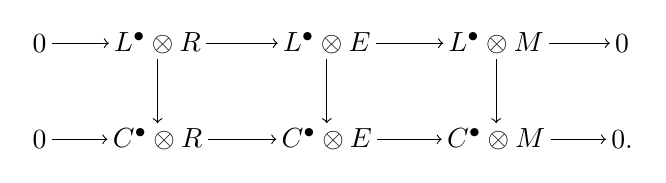
\begin{tikzpicture}[baseline=(current bounding box.center),inner sep=1.75pt]
  \node (a0) at (0,1.22) {$0$}; \node (b0) at (0,0) {$0$};
  \node (a1) at (1.5,1.22) {$L^\bullet\otimes R$};
  \node (b1) at (1.5,0) {$C^\bullet\otimes R$};
  \node (a2) at (3.65,1.22) {$L^\bullet\otimes E$};
  \node (b2) at (3.65,0) {$C^\bullet\otimes E$};
  \node (a3) at (5.8,1.22) {$L^\bullet\otimes M$};
  \node (b3) at (5.8,0) {$C^\bullet\otimes M$};
  \node (a4) at (7.4,1.22) {$0$}; \node (b4) at (7.4,0) {$0$.};
  \foreach \x/\y in {0/1,1/2,2/3,3/4}{
    \draw[->] (a\x) -- (a\y); \draw[->] (b\x) -- (b\y);
  }
  \foreach \x in {1,2,3}{\draw[->] (a\x) -- (b\x);}
\end{tikzpicture}
\]
Applying $h^i$, we get a commutative diagram of long exact sequences. Since the result holds for $i+1$ by induction, and for $E$, since $E$ is free, and $h^i(L^\bullet)\to h^i(C^\bullet)$ is an isomorphism, \EditionText{the diagram gives surjectivity for every finitely generated $M$. In particular, surjectivity holds for $R$, which is finitely generated because $A$ is noetherian. The same diagram then gives injectivity for $M$.}

\medskip
Now we will study conditions under which one of the functors $T^i$ is left exact, right exact, or exact. For any complex $N^\bullet$, we define
\[
 W^i(N^\bullet)=\operatorname{coker}(d^{i-1}\colon N^{i-1}\to N^i)
\]
so that we have an exact sequence
\[
 0\to h^i(N^\bullet)\to W^i(N^\bullet)\to N^{i+1}.
\]

\AuditItem{result-III-12.4}{Proposition 12.4.} \emph{The following conditions are equivalent:}
\begin{enumerate}[label=(\roman*),leftmargin=2.5em,itemsep=0pt,topsep=1pt,parsep=0pt]
\item\hypertarget{result-III-12.4i}{} \emph{$T^i$ is left exact;}
\item\hypertarget{result-III-12.4ii}{} \emph{$W^i=W^i(L^\bullet)$ is a projective $A$-module;}
\item\hypertarget{result-III-12.4iii}{} \emph{there is a finitely generated $A$-module $Q$, such that}
\[
 \EditionText{T^i(M)\cong\operatorname{Hom}_A(Q,M)}
\]
\emph{for all $M$\EditionText{, naturally in $M$}.}
\end{enumerate}
\emph{Furthermore the $Q$ in (\Goto{result-III-12.4iii}{iii}) is unique\EditionText{ up to a unique isomorphism compatible with the representing isomorphisms}.}
}
% Contents from body/page-299.tex.
% Original printed page 285.
\ChapterSheet[11.1]{299}{285}{\Goto{sec-III-12}{12\quad The Semicontinuity Theorem}}{%
\textsc{Proof.}\enspace Since tensor product is right exact, we have
\[
 W^i(L^\bullet\otimes M)=W^i(L^\bullet)\otimes M,
\]
for any $A$-module $M$. We will write simply $W^i$ for $W^i(L^\bullet)$. Hence
\[
 T^i(M)=\ker(W^i\otimes M\to L^{i+1}\otimes M).
\]
Let $0\to M'\to M$ be an inclusion. Then we obtain an exact, commutative diagram
\[
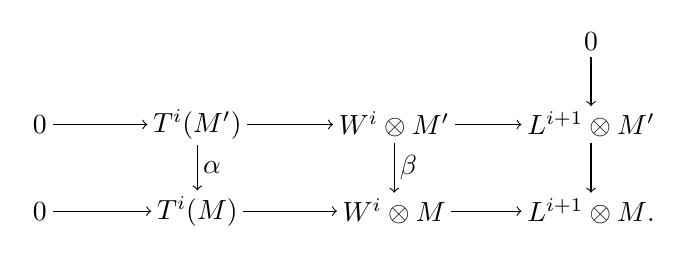
\begin{tikzpicture}[baseline=(current bounding box.center),inner sep=1.9pt]
  \node (z) at (7,2.15) {$0$};
  \node (a0) at (0,1.1) {$0$}; \node (b0) at (0,0) {$0$};
  \node (a1) at (2,1.1) {$T^i(M')$}; \node (b1) at (2,0) {$T^i(M)$};
  \node (a2) at (4.5,1.1) {$W^i\otimes M'$}; \node (b2) at (4.5,0) {$W^i\otimes M$};
  \node (a3) at (7,1.1) {$L^{i+1}\otimes M'$}; \node (b3) at (7,0) {$L^{i+1}\otimes M$.};
  \foreach \x/\y in {0/1,1/2,2/3}{
    \draw[->] (a\x) -- (a\y); \draw[->] (b\x) -- (b\y);
  }
  \draw[->] (a1) -- node[right] {$\alpha$} (b1);
  \draw[->] (a2) -- node[right] {$\beta$} (b2);
  \draw[->] (z) -- (a3);
  \draw[->] (a3) -- (b3);
\end{tikzpicture}
\]
The third vertical arrow is injective, since $L^{i+1}$ is free. A simple diagram chase shows that $\alpha$ is injective if and only if $\beta$ is. Since this is true for any choice of $0\to M'\to M$, we see that $T^i$ is left exact if and only if $W^i$ is flat. (Recall that in any case $T^i$ is exact in the middle (\Goto{result-III-12.1}{12.1}).) But since $W^i$ is finitely generated, this is equivalent to $W^i$ being projective (\Goto{result-III-9.1A}{9.1A}). This shows (\Goto{result-III-12.4i}{i}) $\Leftrightarrow$ (\Goto{result-III-12.4ii}{ii}).

(\Goto{result-III-12.4iii}{iii}) $\Rightarrow$ (\Goto{result-III-12.4i}{i}) is obvious.

To prove (\Goto{result-III-12.4ii}{ii}) $\Rightarrow$ (\Goto{result-III-12.4iii}{iii}), let $\check L^{i+1}$ and $\check W^i$ be the dual projective modules. Define
\[
 Q=\operatorname{coker}(\check L^{i+1}\to\check W^i).
\]
Then for every $A$-module $M$, we have
\[
 0\to\operatorname{Hom}(Q,M)\to\operatorname{Hom}(\check W^i,M)
     \to\operatorname{Hom}(\check L^{i+1},M).
\]
But the last two groups are $W^i\otimes M$, and $L^{i+1}\otimes M$, respectively, so \EditionText{$\operatorname{Hom}_A(Q,M)\cong T^i(M)$ naturally in $M$.}

\EditionText{For uniqueness, let $Q'$ also represent $T^i$. The two representing isomorphisms give
\[
 \operatorname{Hom}_A(Q,M)\cong\operatorname{Hom}_A(Q',M)
\]
naturally in $M$. The image of $1_Q$ and the inverse image of $1_{Q'}$ give maps $Q'\to Q$ and $Q\to Q'$. Naturality shows that the compositions are the respective identities and that the maps are determined by the representing isomorphisms.}
}
% Contents from body/page-300.tex.
% Original printed page 286.
\ChapterSheet[10.95]{300}{286}{\Goto{p-215}{III\quad Cohomology}}{%
\AuditItem{result-III-12.4.1}{\hypertarget{err-5}{}Remark 12.4.1.} There is a general theorem to the effect that any \EditionText{left-exact $A$-linear functor $T$ on $A$-modules, which commutes with arbitrary products, is of the form $\operatorname{Hom}_A(Q,\cdot)$} for some $A$-module $Q$. But even if $T$ takes finitely generated modules into finitely generated modules, $Q$ need not be finitely generated. Thus the fact that our $Q$ in (\Goto{result-III-12.4iii}{iii}) above is finitely generated is a strong fact about the functor $T^i$.

For example, let $A$ be a noetherian ring with infinitely many maximal ideals $\mathfrak m_i$. Let $Q=\sum A/\mathfrak m_i$, and let $T$ be the functor $\operatorname{Hom}(Q,\cdot)$. Then $Q$ is not finitely generated, but for any finitely generated $A$-module $M$, $T(M)$ is finitely generated, because $\operatorname{Hom}(A/\mathfrak m_i,M)\ne0$ if and only if $\mathfrak m_i\in\operatorname{Ass}M$, which is a finite set.

\AuditItem{result-III-12.5}{Proposition 12.5.} \emph{For any $M$, there is a natural map}
\[
 \varphi\colon T^i(A)\otimes M\to T^i(M).
\]
\emph{Furthermore, the following conditions are equivalent:}
\begin{enumerate}[label=(\roman*),leftmargin=2.5em,itemsep=0pt,topsep=1pt,parsep=0pt]
\item\hypertarget{result-III-12.5i}{} \emph{$T^i$ is right exact;}
\item\hypertarget{result-III-12.5ii}{} \emph{$\varphi$ is an isomorphism for all $M$;}
\item\hypertarget{result-III-12.5iii}{} \emph{$\varphi$ is surjective for all $M$.}
\end{enumerate}

\noindent\textsc{Proof.}\enspace Since $T^i$ is a functor, we have a natural map, for any $M$,
\[
 M=\operatorname{Hom}(A,M)\xrightarrow{\psi}\operatorname{Hom}(T^i(A),T^i(M)).
\]
This gives $\varphi$, by setting
\[
 \varphi(\sum a_i\otimes m_i)=\sum\psi(m_i)a_i.
\]
Since $T^i$ and $\otimes$ commute with direct limits, it will be sufficient to consider finitely generated $A$-modules $M$. Write
\[
 A^r\to A^s\to M\to0.
\]
Then we have a diagram
\[
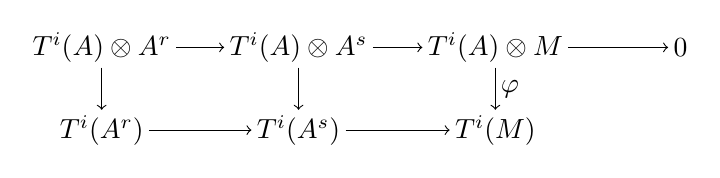
\begin{tikzpicture}[baseline=(current bounding box.center),inner sep=1.75pt]
  \node (a1) at (0,1.05) {$T^i(A)\otimes A^r$};
  \node (b1) at (0,0) {$T^i(A^r)$};
  \node (a2) at (2.5,1.05) {$T^i(A)\otimes A^s$};
  \node (b2) at (2.5,0) {$T^i(A^s)$};
  \node (a3) at (5,1.05) {$T^i(A)\otimes M$};
  \node (b3) at (5,0) {$T^i(M)$};
  \node (a4) at (7.35,1.05) {$0$};
  \draw[->] (a1) -- (a2); \draw[->] (a2) -- (a3); \draw[->] (a3) -- (a4);
  \draw[->] (b1) -- (b2); \draw[->] (b2) -- (b3);
  \draw[->] (a1) -- (b1); \draw[->] (a2) -- (b2);
  \draw[->] (a3) -- node[right] {$\varphi$} (b3);
\end{tikzpicture}
\]
where the bottom row is not necessarily exact. The first two vertical arrows are isomorphisms. Thus, if $T^i$ is right exact, $\varphi$ is an isomorphism. This proves (\Goto{result-III-12.5i}{i}) $\Rightarrow$ (\Goto{result-III-12.5ii}{ii}). The implication (\Goto{result-III-12.5ii}{ii}) $\Rightarrow$ (\Goto{result-III-12.5iii}{iii}) is obvious, so we have only to prove (\Goto{result-III-12.5iii}{iii}) $\Rightarrow$ (\Goto{result-III-12.5i}{i}). We must show if
\[
 0\to M'\to M\to M''\to0
\]
is an exact sequence of $A$-modules, then
\[
 T^i(M')\to T^i(M)\to T^i(M'')\to0
\]
}
% Contents from body/page-301.tex.
% Original printed page 287.
\ChapterSheet[11.15]{301}{287}{\Goto{sec-III-12}{12\quad The Semicontinuity Theorem}}{%
is exact. By (\Goto{result-III-12.1}{12.1}) it is exact in the middle, so we have only to show that $T^i(M)\to T^i(M'')$ is surjective. This follows from the diagram
\[
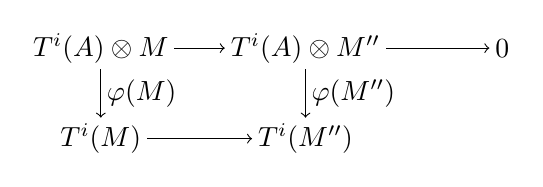
\begin{tikzpicture}[baseline=(current bounding box.center),inner sep=2pt]
  \node (a) at (0,1.15) {$T^i(A)\otimes M$};
  \node (b) at (2.6,1.15) {$T^i(A)\otimes M''$};
  \node (e) at (5.1,1.15) {$0$};
  \node (c) at (0,0) {$T^i(M)$};
  \node (d) at (2.6,0) {$T^i(M'')$};
  \draw[->] (a) -- (b); \draw[->] (b) -- (e);
  \draw[->] (a) -- node[right] {$\varphi(M)$} (c);
  \draw[->] (b) -- node[right] {$\varphi(M'')$} (d);
  \draw[->] (c) -- (d);
\end{tikzpicture}
\]
and the fact that $\varphi(M'')$ is surjective.

\AuditItem{result-III-12.6}{Corollary 12.6.} \emph{The following conditions are equivalent:}
\begin{enumerate}[label=(\roman*),leftmargin=2.5em,itemsep=0pt,topsep=1pt,parsep=0pt]
\item \emph{$T^i$ is exact;}
\item \emph{$T^i$ is right exact, and $T^i(A)$ is a projective $A$-module.}
\end{enumerate}

\noindent\textsc{Proof.}\enspace In any case, $T^i$ is right exact, so by (\Goto{result-III-12.5}{12.5}) we have $T^i(M)\cong T^i(A)\otimes M$ for all $A$-modules $M$. Therefore $T^i$ is exact if and only if $T^i(A)$ is flat. But $T^i(A)$ is a finitely generated $A$-module, so this is equivalent to being locally free (\Goto{result-III-9.1A}{9.1A}), hence projective.

\medskip
Now we wish to localize the above discussion. For any point $y\in Y=\operatorname{Spec}A$, we denote by $T^i_y$ the restriction of the functor $T^i$ to the category of $A_{\mathfrak p}$-modules, where $\mathfrak p\subseteq A$ is the prime ideal corresponding to $y$. Then we say \textquotedblleft $T^i$ is left exact at $y$\textquotedblright\ to mean $T^i_y$ is left exact, and similarly for right exact, or exact. Note that for any $A_{\mathfrak p}$-module $N$, $T^i_y(N)=h^i(L^\bullet_{\mathfrak p}\otimes N)$. Also note that $T^i$ is left exact if and only if it is left exact at all points $y\in Y$; similarly for right exact, or exact. Finally, since cohomology commutes with flat base extension (\Goto{result-III-9.3}{9.3}), we see that $T^i_y$ is the functor $T^i$ associated with the morphism $f'\colon X'\to Y'$ obtained from $f$ by the flat base extension $Y'=\operatorname{Spec}\mathcal O_y\to Y$. So we can apply the results (\Goto{result-III-12.4}{12.4}), (\Goto{result-III-12.5}{12.5}), (\Goto{result-III-12.6}{12.6}) locally to each $T^i_y$.

\AuditItem{result-III-12.7}{Proposition 12.7.} \emph{If $T^i$ is left exact (respectively, right exact, exact) at some point $y_0\in Y$, then the same is true for all points $y$ in a suitable open neighborhood $U$ of $y_0$.}

\par\smallskip\noindent\textsc{Proof.}\enspace $T^i$ is left exact at $y_0$ if and only if $\widetilde W^i_{y_0}$ is free, by (\Goto{result-III-12.4}{12.4}). But since $\widetilde W^i$ is a coherent sheaf on $Y$, this implies that $\widetilde W^i$ is locally free in some neighborhood $U$ of $y_0$, and so $T^i$ is left exact at all points of $U$.

$T^i$ is right exact at a point $y$ if and only if $T^{i+1}$ is left exact there, by the long exact sequence (\Goto{result-III-12.1}{12.1}). So the second statement follows from the first, applied to $T^{i+1}$.

$T^i$ is exact at a point if and only if it is both left exact and right exact, so the third statement is the conjunction of the first two.

\par\smallskip\noindent\textbf{Definition.}\enspace Let $Y$ be a topological space. A function $\varphi\colon Y\to\mathbf Z$ is \emph{upper semicontinuous} if for each $y\in Y$, there is an open neighborhood $U$ of $y$, such that for all $y'\in U$, $\varphi(y')\leqslant\varphi(y)$. Intuitively, this means that $\varphi$ may get bigger at special points.
}
% Contents from body/page-302.tex.
% Original printed page 288.
\ChapterSheet[11.1]{302}{288}{\Goto{p-215}{III\quad Cohomology}}{%
\AuditItem{result-III-12.7.1}{Remark 12.7.1.} A function $\varphi\colon Y\to\mathbf Z$ is upper semicontinuous if and only if for each $n\in\mathbf Z$, the set $\{y\in Y\mid\varphi(y)\geqslant n\}$ is a closed subset of $Y$.

\AuditItem{result-III-12.7.2}{Example 12.7.2.} Let $Y$ be a noetherian scheme, and let $\mathcal F$ be a coherent sheaf on $Y$. Then the function
\[
 \varphi(y)=\dim_{k(y)}(\mathcal F\otimes k(y))
\]
is upper semicontinuous. Indeed, by Nakayama's lemma, $\varphi(y)$ is equal to the minimal number of generators of the $\mathcal O_y$-module $\mathcal F_y$. But if $s_1,\ldots,s_r\in\mathcal F_y$ form a minimal set of generators, they extend to sections of $\mathcal F$ in some neighborhood of $y$, and they generate $\mathcal F$ in some neighborhood, because $\mathcal F$ is coherent. So if $y'$ is in that neighborhood, then $\varphi(y')$, which is the minimal number of generators of $\mathcal F_{y'}$, is $\leqslant r=\varphi(y)$.

\par\smallskip\noindent\hypertarget{result-III-12.8}{}\textbf{Theorem 12.8} (Semicontinuity). \emph{Let $f\colon X\to Y$ be a projective morphism of noetherian schemes, and let $\mathcal F$ be a coherent sheaf on $X$, flat over $Y$. Then for each $i\geqslant0$, the function}
\[
 h^i(y,\mathcal F)=\dim_{k(y)}H^i(X_y,\mathcal F_y)
\]
\noindent\emph{is an upper semicontinuous function on $Y$.}

\par\smallskip\noindent\textsc{Proof.}\enspace The question is local on $Y$, so we may assume $Y=\operatorname{Spec}A$ is affine, with $A$ noetherian. Thus we can apply the earlier results of this section. By (\Goto{result-III-9.4}{9.4}) we have
\[
 h^i(y,\mathcal F)=\dim_{k(y)} T^i(k(y)).
\]
As in the proof of (\Goto{result-III-12.4}{12.4}), we have
\[
 T^i(k(y))=\ker(W^i\otimes k(y)\to L^{i+1}\otimes k(y)).
\]
On the other hand, there is an exact sequence
\[
 W^i\to L^{i+1}\to W^{i+1}\to0,
\]
so tensoring with $k(y)$, we obtain a four-term exact sequence
\[
 0\to T^i(k(y))\to W^i\otimes k(y)\to L^{i+1}\otimes k(y)\to W^{i+1}\otimes k(y)\to0.
\]
Therefore, counting dimensions, we have
\[
\begin{aligned}
 h^i(y,\mathcal F)
   &=\dim_{k(y)}W^i\otimes k(y)+\dim_{k(y)}W^{i+1}\otimes k(y)\\
   &\qquad-\dim_{k(y)}L^{i+1}\otimes k(y).
\end{aligned}
\]
Now $W^i$ and $W^{i+1}$ are finitely generated $A$-modules, so by (\Goto{result-III-12.7.2}{12.7.2}) the first two terms of this sum are upper semicontinuous functions of $y$. But $L^{i+1}$ is a free $A$-module, so the last term is a constant function of $y$. Combining, we see that $h^i(y,\mathcal F)$ is upper semicontinuous.

\par\smallskip\noindent\hypertarget{result-III-12.9}{}\textbf{Corollary 12.9} (Grauert). \emph{With the same hypotheses as the theorem, suppose furthermore that $Y$ is integral, and that for some $i$, the function $h^i(y,\mathcal F)$ is constant on $Y$. Then $R^if_*(\mathcal F)$ is locally free on $Y$, and for every $y$ the natural}
}
% Contents from body/page-303.tex.
% Original printed page 289.
\ChapterSheet[11.35]{303}{289}{\Goto{sec-III-12}{12\quad The Semicontinuity Theorem}}{%
\emph{map}
\[
 R^if_*(\mathcal F)\otimes k(y)\to H^i(X_y,\mathcal F_y)
\]
\noindent\emph{is an isomorphism.}

\par\smallskip\noindent\textsc{Proof.}\enspace As above, we may assume that $Y$ is affine. Using the expression for $h^i(y,\mathcal F)$ in the proof of the theorem, we conclude that the functions $\dim W^i\otimes k(y)$ and $\dim W^{i+1}\otimes k(y)$ must both be constant. But this implies (II, \Goto{result-II-8.9}{8.9}) that $\widetilde W^i$ and $\widetilde W^{i+1}$ are both locally free sheaves on $Y$. So by (\Goto{result-III-12.4}{12.4}), $T^i$ and $T^{i+1}$ are both left exact, so $T^i$ is exact, so by (\Goto{result-III-12.6}{12.6}), $T^i(A)$ is a projective $A$-module. But $R^if_*(\mathcal F)$ is just $T^i(A)^\sim$, so it is a locally free sheaf. Finally by (\Goto{result-III-12.5}{12.5}) we see that
\[
 R^if_*(\mathcal F)\otimes k(y)\to H^i(X_y,\mathcal F_y)
\]
is an isomorphism for all $y\in Y$.

\AuditItem{result-III-12.9.1}{Example 12.9.1.} Let $\{X_t\}$ be a flat family of integral curves in $\mathbf P^n_k$, with $k$ algebraically closed. Then for every closed point $t\in T$, $H^0(X_t,\mathcal O_{X_t})=k$. On the other hand, the arithmetic genus $p_a=1-\chi(\mathcal O_{X_t})$ is constant, by (\Goto{result-III-9.10}{9.10}). So we see that in this case the functions $h^0(t,\mathcal O_X)$ and $h^1(t,\mathcal O_X)$ are both constant on $T$.

\AuditItem{result-III-12.9.2}{Example 12.9.2.} In the flat family of (\Goto{result-III-9.8.4}{9.8.4}), we have $h^0(X_t,\mathcal O_{X_t})=1$ if $t\ne0$, and $2$ if $t=0$, because of the nilpotent elements. On the other hand, $h^1(X_t,\mathcal O_{X_t})=0$ for $t\ne0$, since $X_t$ is rational, and $h^1(X_0,\mathcal O_{X_0})=h^1(X_0,(\mathcal O_{X_0})_{\mathrm{red}})=1$, since $(X_0)_{\mathrm{red}}$ is a plane cubic curve. So in this case the functions $h^0,h^1$ both jump up at $t=0$.

\AuditItem{result-III-12.9.3}{Example 12.9.3.} If $\{X_t\}$ is an algebraic family of nonsingular projective varieties over $\mathbf C$, parametrized by a variety $T$, then the functions $h^i(X_t,\mathcal O_{X_t})$ are actually constant for all $i$. The proof of this result requires transcendental methods, namely the degeneration of the Hodge spectral sequence---cf. Deligne \Goto{bib-deligne-4}{[4]}.

\medskip
Now we wish to give some more precise information about when the map
\[
 T^i(A)\otimes k(y)\to T^i(k(y))
\]
is an isomorphism. And here we will use a new ingredient in our proof, namely the theorem on formal functions (\Goto{result-III-11.1}{11.1}).

\AuditItem{result-III-12.10}{Proposition 12.10.} \emph{Assume that for some $i,y$, the map}
\[
 \varphi\colon T^i(A)\otimes k(y)\to T^i(k(y))
\]
\noindent\emph{is surjective. Then $T^i$ is right exact at $y$ (and conversely, by (\Goto{result-III-12.5}{12.5})).}

\par\smallskip\noindent\textsc{Proof.}\enspace By making a flat base extension $\operatorname{Spec}\mathcal O_y\to Y$ if necessary (\Goto{result-III-9.3}{9.3}), we may assume that $y$ is a closed point of $Y$; $A$ is a local ring, with maximal ideal
}
% Contents from body/page-304.tex.
% Original printed page 290.
\ChapterSheet[11.1]{304}{290}{\Goto{p-215}{III\quad Cohomology}}{%
$\mathfrak m$, and $k(y)=k=A/\mathfrak m$. By (\Goto{result-III-12.5}{12.5}), it is sufficient to show that
\[
 \varphi(M)\colon T^i(A)\otimes M\to T^i(M)
\]
is surjective for all $A$-modules $M$. Since $T^i$ and tensor product commute with direct limits, it is sufficient to consider finitely generated $M$.

First, we consider $A$-modules $M$ of finite length, and we show that $\varphi(M)$ is surjective, by induction on the length of $M$. If the length is $1$, then $M=k$, and $\varphi(k)$ is surjective by hypothesis. In general, write
\[
 0\to M'\to M\to M''\to0,
\]
where $M'$ and $M''$ have length less than length $M$. Then using (\Goto{result-III-12.1}{12.1}) we have a commutative diagram with exact rows
\[
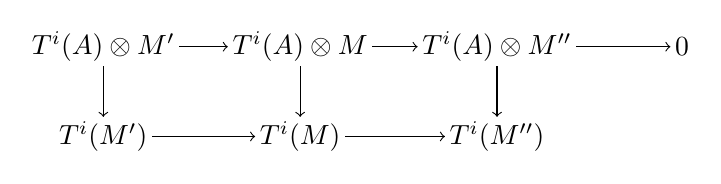
\begin{tikzpicture}[baseline=(current bounding box.center),inner sep=1.5pt]
  \node (a1) at (0,1.14) {$T^i(A)\otimes M'$};
  \node (b1) at (0,0) {$T^i(M')$};
  \node (a2) at (2.5,1.14) {$T^i(A)\otimes M$};
  \node (b2) at (2.5,0) {$T^i(M)$};
  \node (a3) at (5,1.14) {$T^i(A)\otimes M''$};
  \node (b3) at (5,0) {$T^i(M'')$};
  \node (a4) at (7.35,1.14) {$0$};
  \draw[->] (a1) -- (a2); \draw[->] (a2) -- (a3); \draw[->] (a3) -- (a4);
  \draw[->] (b1) -- (b2); \draw[->] (b2) -- (b3);
  \draw[->] (a1) -- (b1); \draw[->] (a2) -- (b2); \draw[->] (a3) -- (b3);
\end{tikzpicture}
\]
The two outside vertical arrows are surjective, by the induction hypothesis, so the middle one is surjective also.

Now let $M$ be any finitely generated $A$-module. For each $n$, $M/\mathfrak m^nM$ is a module of finite length, so that by the previous case,
\[
 \varphi_n\colon T^i(A)\otimes M/\mathfrak m^nM\to T^i(M/\mathfrak m^nM)
\]
is surjective. Note that $\ker\varphi_n$ is an $A$-module of finite length, so the inverse system $(\ker\varphi_n)$ satisfies the Mittag--Leffler condition (II, \Goto{result-II-9.1.2}{9.1.2}). Hence by (II, \Goto{result-II-9.1}{9.1}) the map
\[
 \varprojlim\varphi_n\colon(T^i(A)\otimes M)^\wedge\to\varprojlim T^i(M/\mathfrak m^nM)
\]
is also surjective. But by the theorem on formal functions (\Goto{result-III-11.1}{11.1}), applied to the sheaf $\mathcal F\otimes_A M$ on $X$, the right hand side is just $T^i(M)^\wedge$. So we have a surjection
\[
 (T^i(A)\otimes M)^\wedge\to T^i(M)^\wedge.
\]
Since completion is a faithful exact functor for finitely generated $A$-modules, it follows that
\[
 \varphi(M)\colon T^i(A)\otimes M\to T^i(M)
\]
is surjective, so we are done.

\medskip
Combining this with our earlier results, we obtain the following theorem.

\par\smallskip\noindent\hypertarget{result-III-12.11}{}\textbf{Theorem 12.11} (Cohomology and Base Change). \emph{Let $f\colon X\to Y$ be a projective morphism of noetherian schemes, and let $\mathcal F$ be a coherent sheaf on $X$, flat over $Y$. Let $y$ be a point of $Y$. Then:}

\hypertarget{result-III-12.11a}{}(a) \emph{if the natural map}
\[
 \varphi^i(y)\colon R^if_*(\mathcal F)\otimes k(y)\to H^i(X_y,\mathcal F_y)
\]
}
% Contents from body/page-305.tex.
% Original printed page 291.
\ChapterSheet[10.65]{305}{291}{\Goto{sec-III-12}{12\quad The Semicontinuity Theorem}}{%
\emph{is surjective, then it is an isomorphism, and the same is true for all $y'$ in a suitable neighborhood of $y$;}

\hypertarget{result-III-12.11b}{}(b) \emph{Assume that $\varphi^i(y)$ is surjective. Then the following conditions are equivalent:}
\begin{enumerate}[label=(\roman*),leftmargin=2.9em,itemsep=0pt,topsep=1pt,parsep=0pt]
\item \emph{\EditionText{if $i>0$, $\varphi^{i-1}(y)$ is also surjective};}
\item \emph{$R^if_*(\mathcal F)$ is locally free in a neighborhood of $y$.}
\end{enumerate}

\noindent\textsc{Proof.}\enspace (\Goto{result-III-12.11a}{a}) follows from (\Goto{result-III-12.10}{12.10}), (\Goto{result-III-12.7}{12.7}), and (\Goto{result-III-12.5}{12.5}). (\Goto{result-III-12.11b}{b}) follows from (\Goto{result-III-12.10}{12.10}), (\Goto{result-III-12.6}{12.6}), and (\Goto{result-III-12.5}{12.5}), using the fact that $T^i$ is exact if and only if $T^{i-1}$ and $T^i$ are both right exact\EditionText{ for $i>0$}. \EditionText{For $i=0$, $T^0$ is already left exact.}

\medskip
\emph{References for \S\Goto{sec-III-12}{12}.} The semicontinuity theorem was first proved by Grauert \Goto{bib-grauert-1}{[1]} in the complex-analytic case. These theorems in the algebraic case are due to Grothendieck \Goto{bib-ega-iii}{[EGA III, 7.7]}. Our proof follows the main ideas of Grothendieck's proof, with simplifications due to Mumford \Goto{bib-mumford-5}{[5, II, \S5]}.

\par\medskip\noindent\textsc{Exercises}\par
\AuditItem{ex-III-12.1}{12.1.} Let $Y$ be a scheme of finite type over an algebraically closed field $k$. Show that the function
\[
 \varphi(y)=\dim_k(\mathfrak m_y/\mathfrak m_y^2)
\]
is upper semicontinuous on the set of closed points of $Y$.

\AuditItem{ex-III-12.2}{12.2.} Let $\{X_t\}$ be a family of hypersurfaces of the same degree in $\mathbf P^n_k$. Show that for each $i$, the function $h^i(X_t,\mathcal O_{X_t})$ is a constant function of $t$.

\AuditItem{ex-III-12.3}{12.3.} Let $X_1\subseteq\mathbf P^4_k$ be the \emph{rational normal quartic curve} (which is the $4$-uple embedding of $\mathbf P^1$ in $\mathbf P^4$). Let $X_0\subseteq\mathbf P^3_k$ be a nonsingular rational quartic curve, such as the one in (I, Ex.~\Goto{ex-I-3.18}{3.18b}). Use (\Goto{result-III-9.8.3}{9.8.3}) to construct a flat family $\{X_t\}$ of curves in $\mathbf P^4$, parametrized by $T=\mathbf A^1$, with the given fibres $X_1$ and $X_0$ for $t=1$ and $t=0$.

Let $\mathcal I\subseteq\mathcal O_{\mathbf P^4\times T}$ be the ideal sheaf of the total family $X\subseteq\mathbf P^4\times T$. Show that $\mathcal I$ is flat over $T$. Then show that
\[
 h^0(t,\EditionText{\mathcal I(1)})=
 \begin{cases}0&\text{for }t\ne0\\1&\text{for }t=0\end{cases}
\]
and also
\[
 h^1(t,\EditionText{\mathcal I(1)})=
 \begin{cases}0&\text{for }t\ne0\\1&\text{for }t=0.\end{cases}
\]
This gives another example of cohomology groups jumping at a special point.

\AuditItem{ex-III-12.4}{12.4.} Let $Y$ be an integral scheme of finite type over an algebraically closed field $k$. Let $f\colon X\to Y$ be a flat projective morphism whose fibres are all integral schemes. Let $\mathcal L,\mathcal M$ be invertible sheaves on $X$, and assume for each $y\in Y$ that $\mathcal L_y\cong\mathcal M_y$ on the fibre $X_y$. Then show that there is an invertible sheaf $\mathcal N$ on $Y$ such that $\mathcal L\cong\mathcal M\otimes f^*\mathcal N$. [\emph{Hint:} Use the results of this section to show that $f_*(\mathcal L\otimes\mathcal M^{-1})$ is locally free of rank $1$ on $Y$.]

\AuditItem{ex-III-12.5}{12.5.} Let $Y$ be an integral scheme of finite type over an algebraically closed field $k$. Let $\mathcal E$ be a locally free sheaf\EditionText{ of finite rank at least $2$} on $Y$, and let $X=\mathbf P(\mathcal E)$---see (II, \S\Goto{sec-II-7}{7}). Then show that $\operatorname{Pic}X\cong(\operatorname{Pic}Y)\times\mathbf Z$. This strengthens (II, Ex.~\Goto{ex-II-7.9}{7.9}).
}
% Contents from body/page-306.tex.
% Original printed page 292.
\ChapterSheet[11.5]{306}{292}{\Goto{p-215}{III\quad Cohomology}}{%
\AuditItem{ex-III-12.6}{*12.6.} Let $X$ be an integral projective scheme over an algebraically closed field $k$, and assume that $H^1(X,\mathcal O_X)=0$. Let $T$ be a connected scheme of finite type over $k$.
\begin{enumerate}[label=(\alph*),leftmargin=2.7em,itemsep=0pt,topsep=1pt,parsep=0pt]
\item If $\mathcal L$ is an invertible sheaf on $X\times T$, show that the invertible sheaves $\mathcal L_t$ on $X=X\times\{t\}$ are isomorphic, for all closed points $t\in T$.
\item Show that $\operatorname{Pic}(X\times T)=\operatorname{Pic}X\times\operatorname{Pic}T$. (Do \emph{not} assume that $T$ is reduced!) Cf. (IV, Ex.~\Goto{ex-IV-4.10}{4.10}) and (V, Ex.~\Goto{ex-V-1.6}{1.6}) for examples where $\operatorname{Pic}(X\times T)\ne\operatorname{Pic}X\times\operatorname{Pic}T$. [\emph{Hint:} Apply (\Goto{result-III-12.11}{12.11}) with $i=0,1$ for suitable invertible sheaves on $X\times T$.]
\end{enumerate}
}
